\documentclass[a4paper, 10pt, twoside, titlepage, openright, onecolumn, final]{book}

\usepackage{style}

\title{\tb{Topología Elemental}}
\author{Álvaro García Tenorio \and Manuel Navarro García\and Iván Prada Cazalla \and Álvaro Rodríguez García \and Clara Rodríguez Núñez}
\date{\today}

\begin{document}
	\frontmatter
	\maketitle
	\tableofcontents
	%Para este capítulo se usará la abreviatura "pref"
\section*{Prefacio}
%No se hasta que punto es recomendable referenciar el prefacio siendo la chapuza que es.
\label{pref}
Estas notas son una transcripción de las clases de la asignatura ``\ti{Topología Elemental}'', impartidas por Jesús María Ruiz Sancho en el curso 2016--2017 a los cursos de tercero de los Dobles Grados de Matemáticas e Informática y Matemáticas y Física en la facultad de Ciencias Matemáticas de la Universidad Complutense de Madrid (UCM).

\subsection*{Agradecimientos}
	\addcontentsline{toc}{chapter}{Prefacio}
	\mainmatter
	\part{Topología general}	
	%---CAPITULO DOCUMENTADO CON PAUTAS Y PIJOTERÍAS DE ESTILO

%Generalidades:
%--Usar los entornos predefinidos en el style para teoremas y demás.
%--Cuanto más cosas se etiqueten mejor.
%--Nunca usar \\ para saltar de línea, en su lugar, dar a ENTER dos veces.
%--Redactar.
%Cuidado al usar interiores pues es algo que lamentablemente jode el interlineado. Usar el comando reducido \inter cuando se quiera poner un abierto en medio del texto.

%Para este capítulo se usará la abreviatura "etop".
\chapter{Espacios topológicos}
%Todo capítulo será etiquetado con una abreviatura especificada al inicio del archivo.
\label{etop}
%Todo capítulo comienza con una breve introducción, ya sea a modo de breve motivación o a modo de resumen de contenidos (o ambas).
La necesidad del estudio de la proximidad y continuidad, de la forma más abstracta posible, (absteniéndose del uso de la noción de distancia) dio origen a la Topología.

La idea de espacio topológico se comenzó a desarrollar durante los siglos XIX y XX por matemáticos como Fréchet, Kuratowski, Alexandroff y Hausdorff entre otros.

La definición inicial de estos espacios se puede encontrar en el libro \tb{\ti{``Grundzüge der Mengenlehre''}}\footnote{``Teoría abstracta de conjuntos'', publicado en $1914$ por \tb{\ti{Félix Hausdorff}}(1868-1942).} publicado por este último autor.


Al comienzo de este capítulo introducimos la noción moderna de espacio topológico, añadiendo unos cuantos ejemplos, y posteriormente, presentaremos los conjuntos abiertos y cerrados y sus relaciones.%Continuará...
\section{Espacios topológicos. Definición y ejemplos.}
%Etiquetaremos tanto secciones como subsecciones.
\label{etop_definicionEjemplos}
%Es recomendable redactar un poco entre entorno y entorno y soltar un chascarrillo de vez en cuando para dejar reflexionar al lector y que no le parezca un ladrillo.
Comenzamos, como no podía ser de otra manera, definiendo la estructura sobre la que trabajaremos a lo largo de todas estas notas, los llamados espacios topológicos.
%Es recomendable titular cada entorno entre corchetes.
\begin{defi}[Espacio topológico]
	%Cada vez que comencemos un entorno potencialmente referenciable deberá ser etiquetado siguiendo un convenio similar a este.
	\label{etop_def_espacioTopologico}
	%Cada vez que introduzcamos un concepto nuevo es recomendable ponerlo en negrita y cursiva, se puede hacer usando estos comandos, probablemente haya que crear uno más corto porque la verdad que es un poco coñazo.
	Un \tb{\ti{espacio topológico}} es un conjunto arbitrario no vacío $\mc{X}$ equipado con una colección $\T$ de subconjuntos $\mc{U}\subset\mc{X}$ que cumplen las siguientes propiedades:
	%Cuando se está en un entorno es recomendable poner algo de texto antes de un enmerate para que quede mejor.
	\begin{enumerate}
		%Cuando se definen axiomas importantes en el enumerate se sustituyen los números por cosas que llaman la atención (se suele hacer muy pocas veces).
		\item[\tb{T1}] El vacío y el total están en la colección $\T$, es decir, $\{\emptyset, \X\} \subset \T$
		\item[\tb{T2}] La unión arbitraria de conjuntos de $\T$ está en $\T$. Escrito de forma más rigurosa, pero desde luego, menos elegante, 
		$\bigcup_{i\in I}\U_i\in\T$ donde cada $\U_i\in\T$.
		\item[\tb{T3}] La intersección finita de conjuntos de $\T$ está en $\T$. O, dicho de otra forma, $\bigcap_{i=1}^{n}\U_i\in\T$ donde cada $\U_i\in\T$.
	\end{enumerate}
	A menudo hablaremos tan solo de \tbi{espacio} para referirnos a los espacios topológicos.
\end{defi}
%Siempre viene bien algún chascarrillo para liberar tensiones.
Hagamos un par de pequeñas observaciones antes de continuar con nuestro recién empezado viaje cósmico--topológico.
\begin{obs}[Sutilezas]
	\label{etop_obs_sutilezas}
	Se desprende de la definición \ref{etop_def_espacioTopologico} que un espacio topológico no es más que un par $(\X, \T)$. Como es natural, salvo que sea necesario, nos referiremos a un espacio topológico por el conjunto que lo conforma, al igual que hacemos en casi todas las ramas de las matemáticas (Espacios Vectoriales, Grupos, Anillos,...).
\end{obs}
Introducimos ahora un poco de terminología con la que el lector no tiene más remedio que hacerse familiar.
\begin{obs}[Terminología]
	\label{etop_obs_terminologia}
	A la familia de conjuntos $\T$ que conforman un espacio topológico $\X$ se le denomina \tbi{topología} de $\X$.
	
	Asimismo, los conjuntos que constituyen los elementos de $\T$ reciben el nombre de \tbi[conjunto!abierto]{abiertos} de $\X$. Normalmente los denotaremos con las letras $\U$ o $\W$.
	
	Como es evidente, nos referiremos a los elementos de $\X$ como \tbi[punto]{puntos}.
\end{obs}
Introducimos ahora unos pocos ejemplos para irnos familiarizando con el concepto de espacio topológico viendo lo general que puede llegar a ser.
\begin{exa}[Topologías]
	\label{etop_exa_topologias}
	Las demostraciones de que, efectivamente, se cumplen las restricciones impuestas por la definición \ref{etop_def_espacioTopologico}, o bien ya se han hecho en cursos anteriores, o bien se dejan al lector como ejercicio inmediato.
	\begin{enumerate}
		\item Un espacio métrico $(M,d)$ es un espacio topológico con la topología definida por los conjuntos abiertos en el sentido de los espacios métricos, es decir
		%Se pone una estrellita para que no introduzca número, si no ponemos la estrellita debemos etiquetar la ecuación.
		\begin{equation}
		\label{etop_eq_topologiaRn}
		\T = \{\U\subset M\midc \forall x\in\U\ \exists\  \bola_{d}(x,\varepsilon)\subset\U\}
		\end{equation}
		A esta topología la llamamos \tbitop{usual}.
		\item Una topología interesante por su simpleza, y por que dota a cualquier conjunto no vacío $\X$ con estructura de espacio topológico, es la llamada \tbitop{trivial}, que viene definida por \begin{equation}
		\label{etop_eq_topologiaTrivial}
		\T=\{\emptyset, \X\}
		\end{equation}
		\item Siguiendo la idea del ejemplo anterior, pero a la inversa, encontramos una topología que también dota de estructura topológica a cualquier conjunto no vacío $\X$. Esta topología viene dada por
		\begin{equation}
		\label{etop_eq_topologiaDiscreta}
		\T = \partes(\X)
		\end{equation}
		A esta topología la llamaremos \tbitop{discreta}.
		\item Como último ejemplo curioso nos queda la llamada \tbitop{del punto}. Consiste en considerar como abiertos a todos los subconjuntos de un conjunto $\X$ que contengan a un determinado punto $a$. Es decir
		\begin{equation}
		\label{etop_eq_topologiaPunto}
		\T_a = \{\U \subset \X\midc a\in\U\}\cup\{\emptyset\}
		\end{equation}
		
		%Comento este ejemplo porque no se entiende un zipote lo que explicó este señor.
		
		%\item Como topología especial y rara, tomemos cuatro puntos a, b, c, d, siendo a y b cerrados, y c y d abiertos. Este espacio topológico es homótopo a la circunferencia $(S^{1})$ (viendo así que los conjuntos finitos pueden ser muy interesantes, aunque de primeras no nos lo imaginemos).
	\end{enumerate}
	Con lo que ya tenemos una gama lo suficientemente amplia de ejemplos como para ir tirando.
\end{exa}
Para finalizar la sección observamos que en un mismo conjunto $\X$ podemos definir diversas topologías. Dichas topologías pueden ``compararse'' en determinado contexto.
\begin{defi}[Relación de orden entre topologías]
	Consideremos $\T$ y $\T'$ dos topologías definidas sobre un conjunto $\X$.
	
	Si se verifica que $\T \subset \T'$ diremos que $\T$ es más \tbi[topología más gruesa]{gruesa} que $\T'$ y que $\T'$ es más \tbi[topología más fina]{fina} que $\T$.
\end{defi}
En lo que resta de capítulo iremos introduciendo algunos conceptos generales de los que haremos uso de forma constante a lo largo del curso.
\section{Conjuntos abiertos e interior}
\label{etop_entornos}
En esta sección introducimos el concepto de entorno, cuya utilidad inmediata es caracterizar a los conjuntos abiertos de un espacio topológico $\X$.
\begin{defi}[Entorno de un punto]
	\label{etop_def_entorno}
	Un \tbi{entorno} de un punto $a\in\X$ es un conjunto que contiene a un abierto que contiene al punto $a$.
\end{defi}
Normalmente denotaremos con la letra $\V$ a los entornos, esta costumbre se debe a un galicismo. %¿cuál?

Escribamos la definición de entorno \ref{etop_def_entorno} de forma conjuntista para que no quede ninguna duda.

Dado $\V$ es un entorno de $a\in \X$ si existe un abierto $\U$ de forma que
\begin{equation}
\label{etop_eq_entorno}
a\in\U\subset\V
\end{equation}

Como ya adelantamos, se puede usar la noción de entorno para caracterizar a los abiertos, tal y como muestra el siguiente lema.
\begin{lem}[Caracterización de abiertos]
	\label{etop_lem_caracterizacionAbiertos}
	$\U$ es abierto si y solo si es entorno de todos sus puntos.
\end{lem}
\begin{proof}
	Supongamos que $\U$ es abierto, entonces, dado un punto $a\in\U$ es evidente que $\U$ contiene a un abierto (él mismo) que contiene al punto $a$. Luego $\U$ es, trivialmente, entorno de todos sus puntos.
	
	Recíprocamente, si $\U$ es entorno de todos sus puntos, entonces, para cada punto $a\in\U$ se cumple que
	\begin{equation*}
	a\in\U_a\subset\U
	\end{equation*}
	de donde se desprende que
	\begin{equation*}
	A:=\bigcup_{a\in\U}\U_a\subset\U
	\end{equation*}
	Más aún, se da la otra contención, y además, de forma trivial, ya que todo punto de $\U$ pertenece a algún $\U_a$, luego también a la unión de todos. Luego
	\begin{equation*}
	\U=A
	\end{equation*}
	Como la unión arbitraria de abiertos es abierto, $A$ es abierto, con lo que se sigue el resultado.
\end{proof}
En general, un conjunto será entorno de algunos de sus puntos, en principio no de todos. De esta idea surge la siguiente definición.
\begin{defi}[Punto interior]
	\label{etop_def_puntoInterior}
	Dado un conjunto $A\subset\X$, diremos que un punto $a\in\X$ es un \tbi[punto!interior]{punto interior} de $A$ si $A$ es entorno de $a$.
\end{defi}

Esto pretende modelizar matemáticamente la idea de ``estar muy metido dentro de algo''.

Será algo habitual de ahora en adelante tratar de determinar el conjunto de puntos interiores de un determinado conjunto $A\subset\X$, a este conjunto se le denomina \tbi{interior} de $\X$.

Antes de continuar, fijemos unas cuantas notaciones que utilizaremos según el contexto para referirnos al interior de un conjunto.
\begin{equation}
\label{etop_eq_notacionInterior}
\Int_{\X}(A)=\inter{A}=\Int(A)
\end{equation}
Merece la pena notar que el interior de un conjunto puede ser el conjunto vacío, así como que trivialmente se da la desigualdad conjuntista
\begin{equation}
\label{etop_eq_desigualdadInterior1}
\inter{A}\subset A
\end{equation}
Veamos ahora unos resultados elementales, pero a la vez cruciales, del interior de un conjunto.
\begin{lem}[Apertura del interior]
	\label{etop_lem_aperturaInterior}
	El interior de un conjunto $A$ es un abierto.
\end{lem}
\begin{proof}
	Para probar esto haremos uso del lema \ref{etop_lem_caracterizacionAbiertos}, es decir, trataremos de ver que es entorno de todos sus puntos.
	
	En efecto, dado un punto $a\in\inter{A}$, existe un abierto $\U_a\subset A$ de manera que $a\in\U_a$. Luego para ver que $\inter{A}$ es un entorno de $a$ basta demostrar la inclusión $\U_a\subset\inter{A}$, hagámoslo.
	
	Sea $x\in\U_a\subset A$, es claro que $A$ es entorno de $x$, luego $x\in\inter{A}$.
	
	Con lo cual hemos demostrado que $\inter{A}$ es entorno de todos sus puntos.
\end{proof}

El otro resultado elemental que caracteriza al interior de un conjunto $A$, es que es el mayor abierto contenido en $A$.

Presentamos aquí los primeros pasos de la demostración por ser especialmente útiles y omnipresentes en las matemáticas en general.

Como la unión de abiertos es abierto, es claro que una forma de construir el mayor abierto contenido en cierto conjunto es, coleccionar los abiertos contenidos en dicho conjunto y unirlos. Escrito formalmente, tomamos el conjunto
\begin{equation}
\label{etop_eq_mayorAbierto}
B:=\bigcup_{\W\subset A}\W\text{ con $\W$ abierto.}
\end{equation}
Es claro que $B\subset A$, ya que es una unión de conjuntos contenidos en $A$, además, si hubiera un abierto más grande contenido en $A$ que $B$, este pertenecería a la familia de conjuntos que estamos uniendo, lo cual es absurdo.

Presentamos el final de la demostración en forma de lema.
\begin{lem}[Caracterización del interior]
	\label{etop_lem_caracterizacionInterior}
	El interior de un conjunto $A$ es el mayor abierto contenido en $A$.
\end{lem}
\begin{proof}
	Por el lema \ref{etop_lem_aperturaInterior} sabemos que $\inter{A}$ es abierto, luego, por la ecuación \eqref{etop_eq_mayorAbierto} solo queda probar la igualdad
	\begin{equation*}
	\inter{A}=\bigcup_{\W\subset A}\W\subset A
	\end{equation*}
	Y esto es prácticamente trivial. Veámoslo.
	
	Por una parte, $\inter{A}$ es un abierto contenido en $A$, luego está contenido en la unión de los abiertos contenidos en $A$.
	
	Por otra parte, dado $x\in\bigcup_{\W\subset A}\W$, es claro que, como $\bigcup_{\W\subset A}\W\subset A$ es un abierto, $A$ es entorno de $x$, luego $x\in\inter{A}$, lo que concluye la demostración.
\end{proof}

El lema \ref{etop_lem_caracterizacionInterior} es bastante fuerte y produce algunos corolarios interesantes que presentamos a modo de observaciones.
\begin{obs}[Propiedades del interior]
	\label{etop_obs_propiedadesInterior}
	Enumeramos algunas propiedades del interior.
	\begin{enumerate}
		\item El interior del interior de un conjunto es el interior de dicho conjunto. Si lo escribimos sin que suene como un trabalenguas tenemos
		\begin{equation}
		\label{etop_eq_dobleInterior}
		\inter{\inter{A}}=\inter{A}
		\end{equation}
		Esto es trivial ya que al ser $\inter{A}$ un abierto, el mayor abierto contenido en él es él mismo.
		\item Un conjunto es abierto si y solo si coincide con su interior, es decir
		\begin{equation}
		\label{etop_eq_abiertoInterior}
		A=\inter{A}
		\end{equation}
		Esto es cierto por la misma razón que lo es la ecuación \eqref{etop_eq_dobleInterior}.
		\item Los interiores preservan las contenciones. O lo que es lo mismo
		\begin{equation}
		\label{etop_eq_interiorContencion}
		A\subset B\ra \inter{A}\subset\inter{B}
		\end{equation}
		Por la desigualdad \eqref{etop_eq_desigualdadInterior1} es claro que $\inter{A}\subset B$, y como $\inter{B}$ es el mayor abierto contenido en $B$, y $\inter{A}$ es un abierto contenido en $B$, es claro que $\inter{A}\subset\inter{B}$.
	\end{enumerate}
	Esto ya nos da cierta artillería para defendernos con estos conjuntos.
\end{obs}
Con esto podemos decir que ya hemos liquidado todo lo referente a conjuntos abiertos.
\section{Conjuntos cerrados y adherencia}
\label{etop_cerradosAdherencia}
En esta sección estudiaremos los conjuntos cerrados.

Cabe destacar que la noción de ser cerrado no es exactamente la contraria a la de ser abierto, ya que, como veremos más adelante, hay conjuntos que no son ni abiertos ni cerrados así como conjuntos que son abiertos y cerrados a la vez.

\begin{defi}[Conjunto cerrado]
	Un conjuto $\F$ de un espacio topológico $\X$ se dice \tbi[conjunto!cerrado]{cerrado} si su complementario, $\X\setminus\F$, es abierto.
\end{defi}

Usualmente denotaremos a los conjuntos cerrados con las letras $\F$ o $\mc{H}$.

Usando propiedades básicas de teoría de conjuntos se obtienen algunas propiedades elementales de los conjuntos cerrados.
\begin{lem}[Propiedades de los cerrados]
	\label{etop_lem_propiedadesCerrados}
	Dado un espacio topológico $\X$ se verifica
	\begin{enumerate}
		\item El vacío y el total son cerrados.
		\item La intersección arbitraria de cerrados es cerrada.
		\item La unión finita de cerrados es cerrada.
	\end{enumerate}
\end{lem}
\begin{proof}Vayamos caso por caso.
	\begin{enumerate}
		\item $\X$ es cerrado pues $\X\setminus\X=\emptyset$ es abierto.
		
		Asimismo, $\emptyset$ es cerrado pues $\X\setminus\emptyset=\X$ es abierto.
		\item $\bigcap_{i\in I}\F_i$ es cerrado ya que
		\begin{equation*}
		\X\setminus\left(\bigcap_{i\in I}\F_i\right)=\bigcup_{i\in I}\X\setminus\F_i
		\end{equation*}
		es abierto por ser la unión arbitraria de abiertos un abierto.
		\item $\bigcup_{i=1}^n\F_i$ es cerrado, basta tomar el complementario y ver que es abierto por ser intersección finita de abiertos.
		\begin{equation*}
		\X\setminus\left(\bigcup_{i=1}^{n}\F_i\right)=\bigcap_{i=1}^n\X\setminus\F_i
		\end{equation*}
	\end{enumerate}
	Con lo que concluye la demostración.
\end{proof}
\begin{obs}[Abiertos y cerrados a la vez]
	\label{etop_obs_abiertoCerrado}
	Basta con mirar con atención este lema \ref{etop_lem_propiedadesCerrados} para darse cuenta de que hemos encontrado dos conjuntos que son abiertos y cerrados a la vez, el vacío y el total.
	
	Estos conjuntos abiertos y cerrados a la vez (o ``\tbi[clopen]{clopens}'', del inglés close--open) son de vital importancia a la hora de estudiar la conexión, como veremos más adelante. 
\end{obs}
%----DEJO ESTO COMENTADO HASTA QUE SE DE LA DEFINICIÓN DE COMPACTO----
%Una breve anotación que nos será útil en el futuro. Para la comprobación de compacidad en un computo, nos será útil la utilización de cerrados. Veamos un ejemplo, introducido para motivar esta observación.\\
%\textbf{\underline{Ejemplo}}\\
%\\
%$\cx = \bigcup_{i \in I}\cup_{i} \Rightarrow \cx = \cu_{i_{1}} \cup \ldots \cup \cu_{i_{k}}$ por definición de compacto, que se verá más adelante. Pasando a complementarios tenemos:\\
%$\emptyset = \bigcap_{i \in I}\cf_{i} \Rightarrow \emptyset = \cf_{i_{1}} \cap \ldots \cap \cf_{i_{k}}$.\\
%Por lo tanto para ser compacto el conjunto, la unión de cerrados pertenecientes al conjunto finita a de ser el vacío.\\
%Veamos un caso en el que no se cumple:\\
%$\emptyset = \bigcap(0,\frac{1}{n}] \subset (0,\infty)$. Estos conjuntos son cerrados en este espacio. Pero observamos trivialmente que cualquier $n_0$ finito que coja, la intersección va a dar no vacía, luego el conjunto no es compacto.
%----FIN----
Introducimos ahora un concepto elemental pero interesante, el concepto de puntos adherentes y adherencia.
\begin{defi}[Punto adherente]
	\label{etop_defi_puntoAdherente}
	Un punto $a\in\X$ se dice \tbi[punto!adherente]{adherente} a un conjunto $A\subset\X$ si todo entorno de $a$ corta al conjunto $A$.
	
	Esta definición pretende modelizar la idea de estar ``muy pegado'' a algo.
\end{defi}

\begin{obs}[Definición equivalente]
	\label{etop_defi_equivalente}
	Podríamos haber sustituido la definición \ref{etop_defi_puntoAdherente} por una igual pero cambiando la palabra entorno por la palabra abierto.
	
	La comprobación de que esto se puede hacer es inmediata y se deja al lector.
\end{obs}
Como ya es habitual, coleccionaremos los puntos adherentes a un conjunto dado y estudiaremos las propiedades del conjunto de puntos adherentes. Introduzcamos una definición para verlo formalmente.
\begin{defi}[Adherencia]
	\label{etop_defi_adherencia}
	Se define la \tbi{adherencia} o \tbi{clausura} de un conjunto $A\subset\X$ como el conjunto de los puntos adherentes de $A$.
\end{defi}

Usualmente denotaremos a la adherencia de alguna de las siguientes formas
\begin{equation}
\label{etop_eq_adherencia}
\Adh_{\X}(A)=\Adh(A)=\adher{A}
\end{equation}

Vamos a desgranar ahora una serie de resultados que nos van a hacer ver que adherencia e interior de un conjunto son, de alguna manera, conceptos duales.

Comenzamos en primer lugar con algo casi trivial.
\begin{obs}[Adherencia y conjunto]
	\label{etop_obs_adherenciaConjunto}
	Es claro que se verifica que
	\begin{equation}
	\label{etop_eq_adherenciaConjunto}
	A\subset\adher{A}
	\end{equation}
	Esto es debido a que, evidentemente, cualquier entorno de $a$ contiene al punto $a$, luego, por definición, corta al conjunto $A$.
	
	Visto en perspectiva, esta desigualdad es de alguna manera la dual a la \eqref{etop_eq_desigualdadInterior1}.
	
	Además, combinando ambas desigualdades obtenemos que un conjunto siempre queda ``ensandwichado'' entre su interior y su adherencia.
	\begin{equation*}
		\inter{A}\subset A\subset\adher{A}
	\end{equation*}
	Lo cual puede resultar de utilidad.
\end{obs}

\begin{lem}[Clausura de la adherencia]
	\label{etop_lem_clausuraAdherencia}
	La adherencia de un conjunto $A$ es un cerrado.
\end{lem}
\begin{proof}
	Usaremos lo único que tenemos, es decir, la definición de conjunto cerrado. Por ende, probaremos que $\X\setminus\adher{A}$ es abierto, para lo cual veremos que es entorno de todos sus puntos, haciendo buen uso del lema \ref{etop_lem_caracterizacionAbiertos}.
	
	Dado $x\in\X\setminus\adher{A}$, como $x$ no es un punto adherente, entonces existirá un entorno $\V(\ni x)$, el cual podemos escoger abierto sin pérdida de generalidad tal que se verifica
	\begin{equation*}
	\V\cap A=\emptyset
	\end{equation*}
	Si consiguiéramos demostrar que se de la igualdad
	\begin{equation*}
	\V\cap \adher{A}=\emptyset
	\end{equation*}
	habríamos acabado ya que tendríamos que $x\in\V\subset\X\setminus\adher{A}$, que es, por definición que $\X\setminus \adher{A}$ sea entorno de $x$.
	
	En efecto, la comprobación de esta igualdad es muy fácil, ya que, si tomamos un $y\in\V$, al ser $\V$ abierto, es entorno de $y$.
	
	Por tanto, tendríamos que el punto $y$ no es adherente, ya que existe un entorno, el propio $\V$ que no corta con el conjunto $A$, incumpliendo así la definición \ref{etop_defi_puntoAdherente}.
\end{proof}
Continuamos esta dualización de conceptos dándonos cuenta de que la adherencia es el menor cerrado que contiene a $A$. Como antes, parte de la demostración se basa en un procedimiento estándar que pasamos a explicar.

Es fácil darse cuenta de que, como la intersección arbitraria de cerrados es un cerrado, el menor conjunto cerrado que contiene a uno dado puede ser construido de la siguiente manera
\begin{equation}
\label{etop_eq_menorCerrado}
B:=\bigcap_{\mc{H}\supset A}\mc{H}
\end{equation}
En efecto es un conjunto que contiene a $A$ ya que todos los conjuntos de la familia a intersecar contienen a $A$, además, es el menor de ellos, ya que, de haber uno más pequeño, pertenecería a la familia que se está intersecando, lo cual es absurdo (¡compruébese!).

Presentamos, otra vez, en forma de lema, el resto de la demostración.
\begin{lem}[Caracterización de la adherencia]
	\label{etop_lem_caracterizacionAdherencia}
	La adherencia de un conjunto $A$ es el menor cerrado que contiene a $A$.
\end{lem}
\begin{proof}
	Por la ecuación \eqref{etop_eq_menorCerrado} la demostración se reduce a comprobar que
	\begin{equation*}
	\adher{A}=\bigcap_{\mc{H}\supset A}\mc{H}
	\end{equation*}
	Y esto es una comprobación inmediata.
	
	Por un lado, como $\adher{A}$ es un cerrado que contiene a $A$, es claro que $\adher{A}$ se encuentra en la familia a intersecar, luego contiene a la intersección de la familia.
	
	Recíprocamente, dado un punto adherente $x$, si hubiera un conjunto $\mc{H}$ de la familia tal que $x\not\in \mc{H}$, entonces tendríamos que $x\in\X\setminus\mc{H}\subset\X\setminus A$.
	
	Como $\mc{H}$ es cerrado, $\X\setminus\mc{H}$ es abierto, y, por tanto existirá un entorno $\V$ de $x$ de manera que \begin{equation*}
	x\in\V\subset\X\setminus\mc{H}\subset\X\setminus A
	\end{equation*}
	
	Y, por ende, $\V\cap A=\emptyset$, contra la definición de punto adherente.
\end{proof}
Presentamos a continuación unas cuantas igualdades conjuntistas que pueden resultar bastante útiles al lector.
\begin{prop}[Complementario de la adherencia]
	\label{etop_prop_compAdher}
	\begin{equation*}
	\X\setminus\adher{A}=\Int(\X\setminus A)
	\end{equation*}
\end{prop}
\begin{proof}
	Procedemos por doble contención.
	\begin{enumerate}
		\item[\bsubset] Sea $z\in\X\setminus\adher{A}$. Como $z$ no es adherente a $A$, por definición \eqref{etop_defi_adherencia} habrá un entorno $\V_z$ de $z$ de manera que $\V_z\cap A=\emptyset$. En particular, podremos extraer un entorno abierto $\U_z$ tal que verifique
		\begin{equation*}
		\U_z\cap A =\emptyset
		\end{equation*}
		Tratamos de demostrar que $z$ es punto interior de $\X\setminus A$, esto es, por definición \eqref{etop_def_puntoInterior}, que $\X\setminus A$ sea entorno de $z$, esto a su vez significa que hay un abierto $\U_z'$ contenido en $\X\setminus A$ de forma que $z\in\U_z'$. Así pues el problema se reduce a encontrar dicho entorno, sin embargo, es trivial comprobar el entorno $\U_z$ anteriormente definido cumple los requisitos.
		\item[\bsetsub] Sea $z\in\Int(\X\setminus A)$, demostremos que $z$ no es adherente a $A$, para lo cual debemos encontrar un entorno de $z$, al que llamaremos $\V_z$, de manera que no corte al conjunto $A$. Esto es trivial, ya que $z$ es punto interior de $\X\setminus A$, luego el propio $\X\setminus A$ es entorno de $z$, y, evidentemente, no corta a $A$.
	\end{enumerate}
	Con lo que concluye la prueba.
\end{proof}

Insistiendo es esta dualidad vía complementación entre abiertos y cerrados, presentamos un corolario inmediato.
\begin{cor}[Complementario del interior]
	\label{etop_cor_compInter}
	\begin{equation*}
	\X\setminus\inter{B}=\Adh(\X \setminus B)
	\end{equation*}
\end{cor}
\begin{proof}
	Nos limitaremos a comprobar que ambos conjuntos tienen el mismo complementario. En efecto, por una parte
	\begin{equation*}
	\X \setminus (\X \setminus \inter{B}) = \inter{B}
	\end{equation*}
	Por otro lado, denotando $A:=\X \setminus B$ tenemos
	\begin{equation*}
	\X \setminus \Adh(\X \setminus B)=\X \setminus \adher{A}\stackrel{\textrm{Prp.\ref{etop_prop_compAdher}}}{=}\Int(\X \setminus A)=\Int(\X \setminus (\X \setminus B))=\Int(B)=\inter{B}
	\end{equation*}
	Con lo que se tiene el resultado.
\end{proof}
Una última identidad notable, un poco más profunda que las anteriores es la que relaciona la unión de las adherencias con la adherencia de las uniones.
\begin{prop}[Unión de adherencias]
	La unión de las adherencias es la adherencia de las uniones.
	\label{etop_prop_unionAdher}
	\begin{equation*}
	\adher{A\cup B}=\adher{A}\cup\adher{B}
	\end{equation*}
\end{prop}
\begin{proof}
	Procedemos por doble contención.
	\begin{enumerate}
		\item[\bsubset] 
		Dado $z\in \adher{A\cup B}$, todo entorno $\V_z$ de $z$ corta a $A\cup B$. Veamos que $z$ es, o bien adherente a $A$, o bien adherente a $B$ (quizá a ambos). Para ello supondremos que no es adherente a ninguno de ellos, es decir, que existe un entorno $\W_z$ de $z$ que no corta ni a $A$ ni a $B$. Si este entorno existiera tampoco cortaría a la unión (compruébese), lo cual es absurdo.
		\item[\bsupset]
		Dado un punto $z\in\adher{A}\cup\adher{B}$, veamos que todo entorno de $\V_z$ de $z$ corta a $A\cup B$. Si no lo hiciera, para cada punto $x\in\V_z$, $x$ no estaría en $A$, luego $A\cap \V_z=\emptyset$. Análogamente ocurriría con $B$, lo cual contradice nuestra hipótesis.
	\end{enumerate}
	Con lo que finaliza la demostración.
\end{proof}
\begin{obs}[Demostración alternativa]
	Una demostración alternativa y quizá más contundente de la proposición \ref{etop_prop_unionAdher} consistiría en usar las propiedades de distributividad de las operaciones conjuntistas.
\end{obs}
Por supuesto, este resultado presenta un dual inmediato.
\begin{cor}[Intersección de interiores]
	El interior de la intersección es la intersección de los anteriores.
	\begin{equation*}
	\Int(A\cap B)=\inter{A}\cap\inter{B}
	\end{equation*}
\end{cor}
\begin{proof}
	Comprobaremos, como ya hicimos anteriormente, que ambos conjuntos tienen el mismo complementario.
	
	Por un lado
	\begin{equation*}
	\X \setminus \Int(A\cap B)=\Adh(X\setminus (A\cap B))
	\end{equation*}
	Recíprocamente
	\begin{multline*}
	\X \setminus (\inter{A}\cap \inter{B})=(\X \setminus \inter{A})\cup(\X \setminus \inter{B})=\Adh(\X \setminus A)\cup \Adh(\X \setminus B))=\\=\Adh((\X \setminus A) \cup (\X \setminus B))=\Adh(X\setminus (A\cap B))
	\end{multline*}
	Así, el resultado se sigue.
\end{proof}
El resultado análogo a la proposición \ref{etop_prop_unionAdher} con la intersección no se da, tal y como muestra el siguiente ejemplo.
\begin{exa}[Cuadrados abiertos]
	\label{etop_ejem_cuadradosAbiertos}
	Si consideramos los conjuntos
	\begin{equation*}
	\begin{array}{cc}
	A:=(0,1)\times(0,1)\qquad&\qquad B:=(1,2)\times(0,1)
	\end{array}
	\end{equation*}
	En $\R^2$ con la topología usual, es fácil demostrar (se deja al lector) que $\adher{A\cap B}=\emptyset$ mientras que $\adher{A}\cap\adher{B}=\{1\}\times[0,1]$.
\end{exa}
Vistas todas estas igualdades, al igual que hicimos en la observación \ref{etop_obs_propiedadesInterior}, caractericemos los conjuntos cerrados a partir del concepto de adherencia.
\begin{prop}[Cerrados y adherencia]
	\label{etop_prop_cerradosAdher}
	Un conjunto es $A$ cerrado si y solo si coincide con su adherencia. Es decir
	\begin{equation*}
	A=\adher{A}
	\end{equation*}
\end{prop}
\begin{proof}
	Si $A$ es cerrado, como $\adher{A}$ es el mayor cerrado contenido en $A$, es claro que se tiene que dar la igualdad $A=\adher{A}$.
	
	Recíprocamente, si se da la igualdad $A=\adher{A}$, como $\adher{A}$ es cerrado, también lo será $A$.
\end{proof}
Añadimos una observación final trivial, simplemente por curiosidad.
\begin{obs}[Doble adherencia]
	Dado un conjunto $A$, se tiene que
	\begin{equation*}
	\adher{A}=\adher{\adher{A}}
	\end{equation*}
	Esto es inmediato ya que, como $\adher{A}$ es un cerrado, coincide con su adherencia.
\end{obs}
\section{Puntos de acumulación y conjuntos densos}
En esta sección presentamos el concepto de punto de acumulación, que es muy útil para trabajar con sucesiones, como veremos más adelante. Además, definiremos la idea de que un conjunto sea denso de varias maneras que nos serán muy útiles a la hora de resolver problemas.
\begin{defi}[Punto de acumulación]
	\label{etop_defi_puntoAcumulacion}
	Dado un conjunto $A$ en un espacio topológico $\X$, se dice que un punto $x\in\X$ es un \tbi[punto!de acumulación]{punto de acumulación} de $A$ si todo entorno de $\V_x$ de $x$ verifica que
	\begin{equation*}
	(\V_x\setminus\{x\})\cap A\not=\emptyset
	\end{equation*}
\end{defi}
\begin{obs}[Definición equivalente]
	Una observación análoga a \ref{etop_defi_equivalente} tienen vigencia aquí también.
\end{obs}
Presentemos un poco de terminología para el conjunto de los puntos de acumulación.
\begin{defi}[Conjunto derivado]
	Al conjunto de los puntos de acumulación de un conjunto $A$ se le denomina \tbi[conjunto!derivado]{conjunto derivado}. Usualmente denotaremos al conjunto derivado por $A'$.
\end{defi}
\begin{obs}[Entornos perforados]
	Cuando consideramos un entorno $\V_x$ de un punto $x\in\X$, a veces (sobre todo cuando hablamos de puntos de acumulación) es útil no considerar el entorno entero, sino el entorno salvo un punto.
	
	Cabe destacar que al conjunto $\V_x\setminus\{x\}$ se le suele denominar \tbi[entorno!perforado]{entorno perforado} o \tbi[entorno!pinchado]{entorno pinchado} de $x$.
\end{obs}
Una propiedad interesante de los conjuntos derivados se presenta en el siguiente lema.
\begin{lem}[Descomposición de la adherencia]
	\label{etop_lem_descomposicion}
	\begin{equation*}
	\adher{A}=A\cup A'
	\end{equation*}
\end{lem}
\begin{proof}
	La demostración es inmediata, procedemos por doble contención.
	\begin{enumerate}
		\item[\bsubset] Veamos que todos los puntos de $\adher{A}\setminus A$ están en $A'$. En efecto, dado un $x\not\in A$ adherente a $A$ se tiene que para todo entorno $\V_x$ de $x$
		\begin{equation*}
		\V_x\cap A\not=\emptyset
		\end{equation*}
		Como $x\not\in A$ se tiene que $(\V_x\setminus\{x\})\cap A\not=\emptyset$, cumpliendo la definición de punto de acumulación.
		\item[\bsupset] Es evidente que $A\subset\adher{A}$, luego solo queda comprobar que $A'\subset \adher{A}$. Esto es trivial y se deja al lector la comprobación.
	\end{enumerate}
	Como queríamos demostrar.
\end{proof}
Parémonos un segundo a reflexionar sobre las implicaciones de este resultado.
\begin{obs}[Acumulación y cerrados]
	Es claro que un conjunto es cerrado si y solo si contiene a todos sus puntos de acumulación.
	
	Esto es consecuencia directa de la proposición \ref{etop_prop_cerradosAdher} y el lema \ref{etop_lem_descomposicion}.
\end{obs}
Cabe señalar que, claramente, esta descomposición, en general, no es un partición, tal y como muestra el siguiente sencillo ejemplo.
\begin{exa}[Disco]
	Si consideramos el disco unidad $D$ en $\R^2$ con la topología usual, es fácil demostrar que sus puntos de acumulación coinciden con su adherencia, con lo que obtenemos que
	\begin{equation}
	\adher{D}\setminus D \subsetneq D'
	\end{equation}
	En general (compruébese) se verifica que $\adher{A}\setminus A\subset A'$.
\end{exa}
Según uno echa un ojo a la definición \ref{etop_defi_puntoAcumulacion} le dan ganas de ver qué pasa con aquellos puntos que no cumplen esta definición por los pelos. Para esto introducimos la siguiente definición.
\begin{defi}[Puntos aislados]
	Se llaman \tbi[punto!aislado]{puntos aislados} de un conjunto $A$, a aquellos puntos de $A$ que no son puntos de acumulación. Es decir, a los puntos $x\in A$ que poseen un entorno que cumple
	\begin{equation*}
	\V_x\cap A = \{x\}
	\end{equation*}
\end{defi}
Por el momento no usaremos mucho esta definición, aunque la dejamos aquí aparcada por si las moscas.

Pasamos ahora a definir el concepto de densidad de un conjunto.
\begin{defi}[Conjunto denso]
	\label{etop_def_denso}
	Decimos que un conjunto $A$ es \tbi[conjunto!denso]{denso} en un espacio topológico $\X$ si la adherencia de $A$ es el propio espacio $\X$. Es decir
	\begin{equation*}
	\adher{A}=\X
	\end{equation*}
\end{defi}
Esta definición es poco manejable en algunas circunstancias. Lo bueno que tiene es que, con relativamente poco esfuerzo podemos dar una definición equivalente en unos términos un poco más sencillos, tal y como muestra la siguiente proposición.
\begin{prop}[Caracterización de la densidad]
	Son equivalentes:
	\begin{enumerate}
		\item $A$ es denso.
		\item Todo abierto no vacío $\U$ contiene algún punto de $A$.
	\end{enumerate}
\end{prop}
\begin{proof} Veamos ambas implicaciones
	\begin{enumerate}
		\item[\bra] Sea $\U$ un abierto de $\X$. Por ser $\U$ abierto, es entorno de todos sus puntos. En particular, si $x\in\U$, $\U$ es entorno de $x$, luego, por ser $A$ denso, $\U\cap A\not= \emptyset$.
		\item[\bla] Sea $x\in X$ un punto cualquiera, tomemos un entorno arbitrario suyo $\V_x$, por definición de entorno, habrá un abierto $\U_x$ que verifique
		\begin{equation*}
		x\in\U_x\subset\V_x
		\end{equation*}
		Como $\U_x$ es abierto, contiene, por hipótesis, algún punto de $A$, luego $\V_x\cap A\not=\emptyset$, cumpliendo así $x$ la definición de punto adherente.
	\end{enumerate}
	Con lo que ya hemos terminado.
\end{proof}
De forma natural surge preguntarse si, como en el caso conocido de $\R^n$, los espacios topológicos en general poseen algún subconjunto numerable denso. La respuesta a esta pregunta es no (como veremos más adelante) razón por la cual surge la siguiente definición.
\begin{defi}[Espacio topológico separable]
	Se dice que un espacio topológico $\X$ es \tbi[espacio!separable]{separable} si posee un subconjunto numerable denso.
\end{defi}

Para afianzar la idea de que en la topología la intuición no parará de tendernos trampas, presentamos el siguiente ejemplo.
\begin{exa}[Espacios separables]
	Recordamos en primer lugar por qué $\R^n$ es separable y después presentamos un ejemplo contraintuitivo.
	\begin{enumerate}
		\item $\Q^n$ es un conjunto denso y numerable en $\R^n$ con la topología usual. La numerabilidad de $\Q^n$ es consecuencia de la numerabilidad de $\Q$ (inducción). Asimismo, la densidad puede probarse fácilmente por inducción sobre $n$.
		\item Dado un conjunto cualquiera $\X$ equipado con la topología de un punto $a\in X$, el espacio topológico $(\X,\T_a)$ es separable (nótese que $a$ es denso y finito).
	\end{enumerate}
	Así se ve que, en espacios topológicos puestos con un poco de mala baba, pasan cosas que nos descarajan la intuición.
\end{exa}
Para finiquitar esta sección presentamos el concepto de frontera de un conjunto, que, de momento, al igual que el concepto de punto aislado, quedará en el baúl de los recuerdos.
\begin{defi}[Frontera de un conjunto]
	Definimos la frontera de un conjunto como los puntos adherentes al conjunto que no son interiores. Dicho de otra forma (e introduciendo notación de paso)
	\begin{equation}
	\Fr(A)=\adher{A}\setminus\inter{A}
	\end{equation}
\end{defi}
Es interesante comprobar que, como parece intuitivo, un conjunto y su complementario comparten frontera.
\begin{lem}[Frontera y complementación]
	\begin{equation*}
		\Fr(\X \setminus A)=\Fr(A)
	\end{equation*}
\end{lem}
\begin{proof}
	Basta hacer uso de algunas de las igualdades conjuntistas probadas anteriormente para darse cuenta de que
	\begin{equation*}
		\Fr(\X \setminus A)=\adher{\X \setminus A}\setminus \Int(\X \setminus A)=\adher{\X \setminus A}\setminus (\X\setminus \adher{A})=(\X\setminus\inter{A})\setminus (\X\setminus \adher{A})
	\end{equation*}
	Sabiendo esto, solo queda comprobar la igualdad conjuntista
	\begin{equation*}
		\adher{A}\setminus\inter{A}=(\X\setminus\inter{A})\setminus (\X\setminus \adher{A})
	\end{equation*}
	La cual es trivial. Si tenemos un punto adherente y no interior, es evidente que este no pertenece al complementario de la adherencia, además, por ser un punto no interior, pertenecerá al complementario del interior.
	
	La igualdad se da por que podemos repetir esta demostración a la inversa (compruébese). 
\end{proof}

Una última cosa que merece la pena observar es que la frontera de un conjunto puede ser vista como la intersección de las adherencias del conjunto y su complementario.
\begin{lem}[Frontera y adherencia]
	\begin{equation*}
		\Fr(A)=\adher{A}\cap\adher{\X \setminus A}
	\end{equation*}
\end{lem}
\begin{proof}
	Sabemos que se cumple
	\begin{equation*}
		\adher{A}\cap\adher{\X \setminus A}=\adher{A}\cap(\X \setminus \inter{A})
	\end{equation*}
	Así pues basta comprobar que $\adher{A}\cap(\X \setminus \inter{A})=\adher{A}\setminus \inter{A}$, lo cual es evidente.
\end{proof}

\section{Bases de entornos}
Al igual que en los espacios vectoriales, para estudiar las aplicaciones lineales nos bastaba con fijarnos en qué les ocurría a los vectores de una base, en los espacios topológicos desarrollamos un concepto similar.
\begin{defi}[Base de Entornos de un Punto]
	\label{etop_bases_entornos}
	Una \tbi[base! de entornos]{base de entornos} de un punto $a\in\X$ es una colección $\Va{a}$ de entornos de $a$ tales que todo entorno de $a$ contiene a alguno de $\Va{a}$.
\end{defi}

Como veremos a continuación, el concepto de base de entornos de un punto nos permitirá estudiar la topología alrededor de ese punto.

Veamos unos cuantos ejemplos para aclarar el concepto.
\begin{exa}[Topología Usual]
	\label{etop_exa_baseUsual}
	Consideremos el espacio topológico $\R^n$ con la topología usual. Asimismo consideremos un punto $a\in\R^n$.
	
	Algunos ejemplos naturales de bases de entornos de $a$ son
	\begin{enumerate}
		\item $\Va{a}:=\{\bola(a,\varepsilon)\tq \varepsilon>0\}$, la base usual de entornos abiertos.
		\item $\adher{\Va{a}}:=\{\adher{\bola}(a,\varepsilon)\tq \varepsilon>0\}$, la base usual de entornos cerrados.
	\end{enumerate}
	La comprobación de que efectivamente son bases de entornos es evidente y se deja al lector (simplemente hay que usar la definición de abierto en el espacio topológico $\R^n$ usual).
	
	Una base de entornos un poco más interesante es la siguiente
	\begin{equation}
		\matheuler{W}_a:=\left\{\bola\left(a,\frac{1}{k}\right)\tq k\geq 1\right\}
	\end{equation}
	Lo interesante de esta base es que es numerable. Más adelante estudiaremos cuándo es posible extraer bases de entornos numerables de un punto.
	
	De nuevo, la comprobación de que efectivamente es un base es evidente, basta usar la propiedad arquimediana de los números reales.
\end{exa}

Presentemos otro ejemplo para que el elector aprenda a digerir este concepto en ambientes un poco más abstrusos y hostiles.
\begin{exa}[Topología del Punto]
	\label{etop_exa_basePunto}
	Consideramos un conjunto no vacío $\X$ y un punto $a\in \X$, a partir de aquí construimos el espacio topológico $\X$ con la topología del punto $a$.
	
	Es curioso observar que una base de entornos de $a$ es el propio conjunto $\{a\}$.
	
	Esto es debido a que en la topología del punto $\{a\}$ es un abierto, y todos los abiertos del espacio topológico contienen a $\{a\}$, luego todo entorno de $a$ contiene a $\{a\}$ (que es entorno de $a$).
	
	Este último párrafo puede parecer un trabalenguas de mal gusto, pero animamos al lector a que lo compruebe por su cuenta.
\end{exa}

Para concluir esta pequeña sección presentamos una definición sobre la cual trabajaremos con detalle en el capítulo \ref{num}.

\begin{defi}[I Axioma de Numerabilidad]
	Decimos que un espacio topológico $(\X,\T)$ es \tbi[primer axioma de numerabilidad]{primer axioma de numerabilidad} (o simplemente I Axioma) si todo punto posee una base de entornos numerable.
\end{defi}
Visto lo visto salta a la vista que algunos de los espacios topológicos que hemos visitado desde nuestra nave del misterio cumplen el primer axioma.
\begin{exa}[Espacios I Axioma]
	A la luz del ejemplo \ref{etop_exa_baseUsual} sabemos que $\R^n$ con la topología usual verifica el primer axioma.
	
	Asimismo el ejemplo \ref{etop_exa_basePunto} nos dice (aunque no directamente, hacen falta algunas comprobaciones que se dejan al lector) que cualquier espacio topológico con la topología de un punto $a\in\X$ verifica el primer axioma de numerabilidad (de hecho podemos encontrar bases finitas de un único entorno).
\end{exa}
En general, los espacios primer axioma son importantes dado que en ellos podremos fabricar sucesiones (y todos los potentes argumentos que se derivan de este hecho).

Por suerte o por desgracia, hay espacios que no verifican el primer axioma. Como veremos más adelante, el espacio topológico de las funciones continuas (con cierta topología) no es primer axioma.

Finalizamos la sección observando que, dada una base de entornos numerable de un punto, podemos obtener una \tbi[base! encajada]{base encajada}. Y además, ¡agárrense criaturas! por que la demostración de este hecho es constructiva.
\begin{obs}[Extracción de una Base Encajada]
	\label{etop_obs_base_encajada}
	Dada una base numerable de un punto $a\in\X$, a la que denotamos
	\begin{equation*}
		\Va{a}:=\{\V_i\tq i\in\N\}
	\end{equation*}
	Es claro que la base $\Va{a}^*:=\{\W_i:=\bigcap_{j=1}^i\V_j\tq i\in\N\}$ es encajada.
	
	Esto es, $\W_k\subset\W_l$ para todo $k\geq l$
\end{obs}
Usaremos esta construcción de forma asidua cuando estudiemos las sucesiones con detalle.
\section{Base de abiertos}
\begin{defi}[Base de abiertos]
	\label{etop_bases_abiertos}
	Una \tbi[base!de abiertos]{base} de $\T$ es una colección $\B$ de abiertos, tal que todo abierto de $\T$ es unión de abiertos de $\B$
\end{defi}

Esto viene a ser una filosofia parecida a la del álgebra lineal, pero cambiando unión por combinación lineal y abiertos por vectores. Ahora vamos a ver una reformulación de este concepto bastante potente, pues relaciona los dos conceptos de base que tenemos hasta el momento.

\begin{prop}[Caracterización de las bases de una topología]
	$\B$ es base de $\T$ si y solo si para cada $x \in \X$ el conjunto
	$\V_x = \{ V \in \B \tq  x \in V\}$ es una base de entornos de x.
\end{prop}
\begin{proof} 
	Supongamos que $\B$ es base de $\T$. Veamos que $\V_x$ es base de entornos de $x$. Para ello, sea $V$ entorno de x. Entonces hay un $\U$ abierto de manera que $x \in \U \subset \V$. Como $\B$ es base de abiertos de $\T$, tenemos que
	$x \in \U = \bigcup_{i \in I, V_i \in \B} V_i \subset V \Rightarrow$ hay un $V_i \in \B$ tal que $x \in V_i \subset \U \subset V$.
	
	Ahora supongamos que $\V_x$ es base de entornos de $x$. Veamos que $\B$ es base de abiertos. Sea $\U$ un abierto no vacío y $x \in \U$. Por ser $V_x$ base de entornos de x y $\U$ entorno de $x$, pues es un abierto que contiene a $x$, habrá un $V \in \V_x$ tal que $x \in V \subset \U$. Como podemos hacer esto para cada $x \in \U$, es fácil deducir que $\U = \bigcup_{x \in \U} V_x$, pues es claro que $V_x \subset \U \ \forall x \Rightarrow \bigcup V_x \subset \U$ y por otro lado $x \in V_x \ \forall x \Rightarrow \U \subset \bigcup V_x$.
\end{proof}

Hechas estas consideraciones, pasemos a ver ejemplos de bases de abiertos.
\begin{exa}[Bases de abiertos]
	En $( \R^n,\T_u )$ todas las siguientes colecciones son bases de abiertos de $\T_u$.
 	 $$\B_1=\{B(x, \varepsilon) \tq x \in \R^n\ y \ \varepsilon > 0\}$$
	 $$\B_2=\{B(x, \frac{1}{k}) \tq x \in \R^n\ y \ k \geq 1\}$$
	 Usando la caracterización vista anteriormente, es trivial comprobar que $B_1$ y $B_2$ efectivamente son bases.
	 $$\B_3=\{B(q, r) \tq q \in \Q^n\ y \ r \in \Q\}$$
	 Esta última es especialmente importante, pues es una base numerable.
\end{exa}

\begin{obs}
	Una vez hallamos demostrado que cierta $\B$ es base de abiertos, para demostrar que $\B'$ es base, basta con expresar los abiertos de $\B$ como unión de los de $\B'$. Por eso es importante encontrar bases lo más pequeñas posibles.  \qedhere
\end{obs}

Tras haber visto bases de abiertos \ref{etop_bases_abiertos} y bases de entornos \ref{etop_bases_entornos}, vamos a plantear el II axioma de numerabilidad, que, aunque será tratado con profundidad en el capítulo \ref{num}, expone muy bien las ideas recién tratadas.
 
\begin{defi}[II axioma de numerabilidad]
	\label{etop_2_axioma_num}
	Diremos que $\X$ es \tbi[segundo axioma de numerabilidad]{segundo axioma} de numerabilidad (o simplemente II axioma) si tiene una base de abiertos numerable.

\end{defi}
\begin{obs}
	Ser II axioma implica ser I axioma. \qedhere
\end{obs}
\begin{proof}
	Si $\B$ es una base numerable para la topología de $\X$, entonces si tomamos el subconjuto de $\B$ formado por los elementos de la base que contienen al punto $x$ entonces es una base numerable en $x$. Luego todo punto tiene una bsae numerable, por lo que es I axioma.
\end{proof}

\begin{obs}
	Ser II axioma implica ser separable. \qedhere
\end{obs}
\begin{proof}
	Hay que ver que en todo abierto hay un punto del conjunto numerable denso. Como todo abierto es unión numerable de abiertos de la base, basta escoger un punto de cada conjunto de la base, habiendo construido así el conjunto numerable denso.
\end{proof}

Hemos de comentar que el II axioma es mucho más fuerte que el I axioma. De hecho no todos los espacios métricos lo cumplen. Será útil ya que muchos espacios que no son familiares lo cumplen, y nos ayudará para probar algunos teoremas. \\

La siguiente proposición responde algunas preguntas importantes.
\begin{prop}[Caracterización de las bases de abiertos]
	\label{etop_base_top}
	Una colección de subconjuntos $\B$ de $X$ es base de una topología si y sólo si se verifican las siguientes condiciones:
	\begin{enumerate}
		\item La base $\B$ cubre todo el espacio, es decir, $X = \bigcup_{B \in \B}B$
		\item Para todo $B_1$, $B_2 \in \B$ y para todo $x \in B_1 \cap B_2$,  $\exists B \in \B$  y  $B \subset B_1 \cap B_2$ tal que $x \in B$.
	\end{enumerate}
\end{prop}
\begin{proof}
	\begin{enumerate}
		Supongamos que $\B$ es base, entonces se cumple 1 trivialmente. Además, $B_1 \cap B_2$ es abierto, luego entorno de $x$, por tanto $\exists B$ tal que $x \in B \subset B_1 \cap B_2$. Luego se cumple 2. \\
		
		Veamos ahora la otra implicación. Si la colección de conjuntos $\T = \{ U \subset X \tq U = \bigcup_{B \in \B}B$ es una topología, entonces $\B$ es base. Vayamos a la demostración. Si $X = \bigcup_{B \in \B}B$ es claro que $\B$ es una base de la topología trivial. Además si se cumple 2, es claro que por construcción $B_1 \cap B_2 \neq \emptyset$. Sean $\U_1, \U_2 \in \T$, supongamos que $\U_1 \cap \U_2 \neq \emptyset$, entonces hay un $x \in \U_1 \cap \U_2$. Esto implica que $\U_1$ y $\U_2$ son entornos de $x$. Como se cumple 2, existen sendos $B_1, B_2$ tales que $x \in B_1 \cap B_2 \subset \U_1 \cap \U_2$. Tomando la unión llegamos al resultado.
	\end{enumerate}
\end{proof}

\begin{exa}[Topología de Sorgenfrey en $\R$]
	Sea el espacio topológico $(\R, \T_s)$ espacio topológico, con $\T_s$ la llamada topología de Sorgenfrey. Veamos en que consiste esta topología. 
	
	Si tomamos en $\R$ la colección de intervalos $[a,b)$, este conjunto es base de la llamada \tbitop{de Sorgenfrey}.
	\begin{proof}
		Para ver que ocurre esto comprobaremos que esta base cumple \ref{etop_base_top}
		
		Denotemos $\B = \{[a,b) : a,b \in \R\}$. Que $\B$ cumple que la unión de todos sus elementos genera el total es obvio($\R$ es la unión de estos intervalos).
		
		Veamos que cumple la segunda propiedad. Sea $\B_1=[a,b)$ y $\B_2=[a',b')$ y sea $x \in B_1 \cap \B_2$ vemos claramente que la intersección de estos dos intervalos sigue siendo de la misma forma, y tendrá como extremo inferior $a" = max\{a,a'\} $ y superior $b"=min\{b,b'\}$ luego es el intervalo $B_1 \cap \B_2 = [a",b")$, por lo que pertenece a la base y se cumple que $x \in B \subset B_1 \cap \B_2$. Luego llegamos a lo buscado.
	\end{proof}
	Veremos una serie de propiedades extra de esta topología, que son muy ilustrativas.
	\begin{enumerate}
		\item Los abiertos de la topología usual están contenidos en la topología de Sorgenfrey.
		\begin{proof}
			Sea el intervalo $(a,b)$. Describamoslo en función de intervalos cerrado-abierto. $(a,b) = \cup_{k\geq 1} [a+\frac{1}{k},b)$. Sabemos que esta unión está en la topología de Sorgenfrey luego ya está.
		\end{proof}
	Con esto observamos que la topología de Sorgenfrey es más fina que la usual $(\T \subsetneq \T_{s})$. Para ver que efectivamente son distintas, basta tomar un abierto de Sorgenfrey $[a,b)$ y darse cuenta de que no es abierto en la usual.
	
	
	Con esto sabemos que si un conjunto no es compacto con la topología de Sorgenfrey tampoco lo es con la usual, ya que si con una que tiene los mismos y más abiertos no podemos extraer un subrecubrimiento finito, difícilmente podremos hacerlo con una más pequeña.
	\item Es una base de conjuntos abiertos y cerrados (lo que se llama una topología "\textit{clopen}")
	\begin{proof}
		Ver esto es muy sencillo. Si tenemos el abierto (en esta topología) $[a,b)$, tenemos que su complementario es $(-\infty, a) \cup [b,\infty)$. El intervalo $(-\infty, a)$ es un abierto de la usual, luego de la de Sorgenfrey, y $[b,\infty)$ lo poedmos escribir como $[b,\infty) = \cup_{k\geq1} [b, b+k)$ que es un abierto Sorgenfrey. Luego el intervalo $[a,b)$ es un abierto-cerrado.
	\end{proof}
	\item No hay conexos(salvo los puntos).
	\item No es II axioma.
	\item Es separable.
	\item Es I axioma (tomamos $[a, a+\frac{1}{k})$).
	\item Es Lindelöf.
	\end{enumerate}
\end{exa}


\section{Topología relativa}

\begin{defi}[Topología relativa]
	Sea $(\X,\T)$ un espacio topológico, y un subconjunto $\mc{Y}\subset\X \neq \emptyset$. Definimos la \tbitop{relativa} en $\mc{Y}$ como $\T\restriction_\mc{Y} = \{U\cap\mc{Y}\colon U\in\T\}$.
	En general, decimos que $(\mc{Y},\T\restriction_\mc{Y})$ es un \tbi{subespacio topológico}. Y a los abiertos de $\mc{Y}$ se les denomina \tbi{abiertos relativos}.
\end{defi}
	
	Comprobemos que efectivamente es una topología. \\
	Contiene el vacío y el total. En efecto, $\emptyset \in \T\restriction_\mc{Y}$ pues $\emptyset \cap \mc{Y} = \emptyset$ y $\mc{Y} \in \T\restriction_\mc{Y}$ pues $\X \cap \mc{Y} = \mc{Y}$. 
	Es cerrado respecto de uniones arbitrarias. En efecto, $\bigcup_{i \in I}{(\U \cap \mc{Y})} = \big( \bigcup_{i \in I} \U \big) \cap \mc{Y}$. Y por último, es cerrado respecto de intersecciones finitas. En efecto, $\bigcap_{i = 1}^{n}{(\U_i \cap \mc{Y})} = \big( \bigcap_{i=1}^{n} \U_i \big) \cap \mc{Y}$. \\

	Gracias a esta definición, siempre que hablemos en adelante de un subconjunto de $\X$ y necesitemos una topología definida en él, se usará por defecto la relativa para dotarlo de estructura de espacio topológico. \\

Veamos ahora un lema referido a resultados más elementales.

\begin{lem}[Bases y topología relativa]
	Sea $Y$ un subconjunto no vacío de $\X$. Entonces:
	\begin{enumerate} 
		\item Si $\V_y$ es base de entornos de $y \in Y$ en $\X$, entonces $\V_y \cap Y$ es base entornos en $Y$.
		\item Si $\B$ es base en $\X$, $\B \cap Y$ es base en $Y$. 	
	\end{enumerate}
\end{lem}

\begin{obs}[Lindelöf y separabilidad]
	Si $\X$ es un espacio Lindelöf o separable, $Y \subset \X$ no tiene porque serlo. \qedhere
\end{obs}

Vamos a ver ahora que la topología relativa también preserva esa ``dualidad'' de la que hablábamos antes entre abiertos y cerrados. En particular, también los cerrados relativos son las intersecciones de los cerrados de $\X$.

\begin{lem}[Cerrados relativos]
	Los cerrados de $\mc{Y}$ son las intersecciones de los cerrados de $\X$ con $\mc{Y}$. Es decir, $C\subset\mc{Y}$ es cerrado si existe $F\subset\X$ cerrado tal que $C = F\cap\mc{Y}$.
	
	\begin{proof}
		Sea $W\subset\X$ un abierto de $X$. Entonces, $\X\setminus W$ es cerrado, y queremos ver si $C=\mc{Y}\cap(\X\setminus W)$ es cerrado. Pero esto es lo mismo que ver si $\mc{Y}\setminus C$ es abierto, y:
		\[\mc{Y}\setminus C=\mc{Y}\setminus (\mc{Y}\cap(\X\setminus W))=\mc{Y}\setminus ((\mc{Y}\cap\X)\setminus W)=\mc{Y}\setminus (\mc{Y}\setminus W) = \mc{Y}\cap W\]
		donde para las igualdades anteriores se han utilizado relaciones conocidas de teoría de conjuntos. Entonces, como $\mc{Y}\cap W$ es abierto por definición de topología relativa, $\mc{Y}\setminus C$ también lo es, y por tanto $C$ es cerrado.
	\end{proof}
\end{lem}

\begin{lem}[Entornos relativos]
	Sea $A \subset \X$. Los entornos de $a \in A$ son las intersecciones de A con los entornos de $a$ en $\X$.	
\end{lem}
\begin{proof}
	Sea $\V$ un entorno de $a$ en $\X$, entonces hay un abierto $\U$ tal que $x \in \U \subset \V$. Veamos que $\V \cap A$ es entorno de $a$ en $\X$. Para ello vemos que hay un abierto $\U'$ tal que $x \in \U' \subset \V \cap A$. Dicho abierto es, intuitivamente, $\U \cap A$.
	Vamos a comprobarlo formalmente. Sea $a \in \U \cap A$. Veamos que $(\U \cap A) \subset (\V \cap A)$. Como $\U \subset \V$, dado $x \in \U $ y $x \in A \Rightarrow x \in \V$ y $ x \in A$. \\
	
	Sea $\V'$ un entorno de $a$ en $A$, entonces hay un abierto $\U'$ tal que $x \in \U' \subset \V'$. Como $\U'$ es abierto relativo en $A$, $a \in \U \cap A \subset \V'$. Veamos que $\V' = \V \cap A$ con $\V$ un entorno de $a$ en $\X$. Es claro que $\U$ es entorno de $a$ en $\X$, por ende, basta tomar $\V = \V' \cap \U$.
\end{proof}

\begin{prop}[Relatividad y adherencias]
	Sea $A \subset \X$ y $\pi \subset A$. Se cumple que $A \supset Adh_A(\pi) = A \cap Adh_{\X}(\pi)$.
\end{prop}
\begin{proof}
	$a \in Adh_A(\pi)$ si y solo si dado un entorno de $a$ en $A$, $\emptyset \neq \V_A \cap \pi = \V_x \cap (A Cap \pi) = \V_x \cap \pi$.
\end{proof}


\begin{obs}[Otras propiedades]
	\begin{enumerate}
		\item Sea $A\subset\X$ abierto. Si $A\cap U$ es un abierto en la topología $\T\restriction_A$ (es decir, $U$ es abierto en $\T_\X$), entonces $A\cap U$ es también abierto en $\T_\X$.
		\item Sea $F\subset\X$ cerrado. Si $F\cap C$ es un cerrado en la topología $\T\restriction_F$ (es decir, $C$ es cerrado en $\T_\X$), entonces $F\cap C$ es también cerrado en $\T_\X$. \qedhere
	\end{enumerate}
\end{obs}

\begin{lem}[Bases relativas]
	Sea $\mc{Y} \subset \X$.
 	\begin{enumerate}
 		\item Si $\V_y$ es base en $\X$, $\V_y \cap \mc{Y}$ es base en $\mc{Y}$.
 		\item Si $\B$ es base en $\X$, $\B \cap \mc{Y}$ es base en $\mc{Y}$.
 	\end{enumerate}
\end{lem}
\begin{proof}
	\begin{enumerate}
		\item Hay que ver que dado un entorno de $y$ en $\mc{Y}$, que son de la forma $V \cap \mc{Y}$, hay uno de la forma $W \cap \mc{Y}$ tal que $(W \cap \mc{Y}) \subset (V \cap \mc{Y})$. Es claro que $W \cap V$ lo cumple.
		\item Dado un abierto $\U$ en $\mc{Y}$, tenemos que $\mc{Y} \cap \U = \mc{Y} \cap \big( \bigcup B \big) = \bigcup (B \cap \mc{Y})$.
	\end{enumerate}
\end{proof}
	%Para este capítulo se usará la abreviatura "cont".
\chapter{Continuidad}
\label{cont}

La continuidad es la propiedad por excelencia que queremos que nuestras funciones verifiquen. En este breve capítulo vamos a generalizar la noción de continuidad que ya conocemos y dominamos para espacios como $\R^n$, de forma que la podamos aplicar a cualquier espacio topológico conocido (sin necesidad de que sea métrico). La continuidad, además, será clave para definir más adelante la noción de homeomorfismo, es decir, una transformación que preserva las propiedades topológicas de un espacio dado.

\section{Definición y propiedades elementales}

Para empezar, tratamos de dar una justificación intuitiva del cómo se llegó a la definición que presentaremos a continuación.

Hasta ahora conocíamos una definición de continuidad válida en el ámbito de los espacios métricos, que nos decía que si $(M,d)$ y $(N,d')$ eran espacios métricos arbitrarios y $f:M\to\N$ una aplicación entre ellos, era continua en un punto $x_0\in M$ si y solo si dado un $\varepsilon>0$ podíamos encontrar un $\delta>0$ de forma que $f(\bola_d(x_0,\delta))\subset\bola_{d'}(f(x_0),\varepsilon)$.

Dicho de otra forma, si cierto punto dista de $x_0$ menos que $\delta$, entonces su imagen deberá distar menos que $\varepsilon$ de la imagen de $x_0$. Informalmente, una aplicación continua es la que manda puntos próximos a puntos próximos.

En los espacios topológicos no tenemos la noción de distancia, pero si cierta noción de ``proximidad'', o al menos de ``ligadura'' entre puntos, esta es la noción de entorno, que usaremos para extender esta definición.
\begin{defi}[Continuidad en un punto]
	Sean $\X$ e $\Y$ espacios topológicos. Consideremos asimismo una aplicación $f:\X\to\Y$.
	
	Diremos que $f$ es \tbi[aplicación!continua]{continua} en un punto $x_0\in\X$ si para todo entorno $V_{f(x_0)}$ de $f(x_0)$, la imagen inversa de dicho entorno, $f^{-1}(V_{f(x_0)})$, es entorno de $x_0$. 
\end{defi}

Dicho con palabras llanas, $f$ es continua en un punto si transforma entornos en entornos por imágenes inversas.

Una forma totalmente equivalente de entender este concepto es pensar que dado un entorno $V_{f(x_0)}$ de $f(x_0)$ siempre podremos encontrar un entorno $V_{x_0}$ de forma que $f(V_{x_0})\subset V_{f(x_0)}$.
\begin{obs}[Importancia de las topologías]
	\label{cont_obs_importanciaTopol}
	Si la topología de $\X$ es fina (con muchos abiertos), o la topología de $\Y$ es muy grosera (con muy pocos abiertos), la continuidad suele ser más fácil de comprobar, ya que hay pocos entornos que chequear en el espacio de llegada y muchos candidatos en el espacio de partida.
\end{obs}
Al hilo de la observación \ref{cont_obs_importanciaTopol} veamos algunos casos extremos que pueden resultar chocantes para una mente poco experimentada en los exóticos placeres topológicos.
\begin{obs}[Casos extremos]
	\label{cont_obs_continuidad_discreta_trivial}
	Veamos cual es el comportamiento de la continuidad con las topologías más drásticas que conocemos.	
	\begin{enumerate}
		\item En la topología discreta, cualquier conjunto es abierto, con lo cual $\{x_0\}$ es abierto y, por tanto, cualquier conjunto que contenga a $x_0$ es entorno suyo. Entonces, para cualquier entorno de $f(x_0)$ su imagen inversa contendrá a $x_0$ y por lo anterior será entorno suyo. Es decir, cualquier función que nazca en $\X$ con la topología discreta es continua.
		
		\item En la topología trivial, los únicos abiertos son el vacío y el total, con lo cual dado un punto, su único entorno es el total. Entonces, si $\Y$ con la topología trivial es el espacio de llegada de una función $f$, $f$ es continua, pues la imagen inversa del total es el total, y este es abierto (y por tanto entorno) en cualquier topología. \qedhere 
	\end{enumerate}
\end{obs}

De la misma forma que podemos estudiar la continuidad para unas ciertas topologías concretas, podemos estudiarla para algunas funciones concretas sin limitarnos a una topología particular. En particular, nos van a interesar la función constante y la función identidad.

\begin{obs}[Aplicaciones constante e identidad] \
	\label{cont_obs_continuidad_cte_e_id}
	\begin{enumerate}
		\item Si $f:\X\to\mc{Y}$ es la aplicación constante $f\equiv b$, entonces $f$ es continua con cualquier topología. En efecto, la imagen inversa de cualquier subconjunto (y en particular de cualquier entorno) de $\mc{Y}$ que contenga a $b$ es el total, que es entorno de todos los puntos (por ser abierto).
		
		\item La continuidad de la aplicación identidad depende de los espacios topológicos sobre los que está definida, al contrario de lo que pueda parecer. Caso curioso es el siguiente:
		\[\text{id}:(\X,\T_\text{discreta})\to (\X,\T_\text{trivial})\]
		Esta aplicación es continua (y biyectiva), por la observación \ref{cont_obs_continuidad_discreta_trivial}. Sin embargo, su inversa, que también es la aplicación identidad, no es continua. Esto se sigue directamente de que, por ser la topología del espacio de llegada la discreta, $\{f(x_0)\}$ es abierto y por tanto entorno de $f(x_0)$, pero su imagen inversa es $\{x_0\}$ que con la topología trivial del espacio de salida no es entorno. \qedhere
	\end{enumerate}
\end{obs}

Ahora, veremos un par de propiedades interesantes de la continuidad en un punto.

\begin{prop}[Continuidad y restricciones]
	Dada $f:\X\to\mc{Y}$, continua en $x_0\in\X$, si $A\subset\X$ tal que $x_0\in A$, entonces $f\restriction_A:A\to\mc{Y}$ es continua en $x_0$.
	
	\begin{proof}
		Sea $V_{f(x_0)}$ un entorno de $f(x_0)$. Se verifica que $(f\restriction_A^{-1})(V_{f(x_0)}) = A\cap f^{-1}(V_{f(x_0)})$. Pero como por la continuidad de $f$ en $x_0$ tenemos que $f^{-1}(V_{f(x_0)})$ es entorno de $x_0$ en $\X$, entonces $A\cap f^{-1}(V_{f(x_0)})$ es entorno de $x_0$ en $A$ (nótese que consideramos la topología relativa en $A$).
	\end{proof}
\end{prop}

	Este lema viene a decirnos que la continuidad no depende del conjunto donde nos encontremos, no obstante, si depende (y mucho) de la topología.
	
	La siguiente proposición es el recíproco de la anterior.

\begin{prop}[Continuidad como propiedad local] Si hay un entorno $V_{x_0}$ de $x_0$ tal que $f\restriction_{V_{x_0}}$ es continua en $x_0$ entonces $f$ es continua.
	
	\begin{proof}
		Sea $V_{f(x_0)}$ un entorno de $f(x_0)$, por continuidad de  $f\restriction_{V_{x_0}}$ en $x_0$ se cumple que $(f\restriction_{V_{x_0}})^{-1}(V_{f(x_0)}) = f^{-1}(V_{f(x_0)})\cap V_{x_0}$ es entorno de $x_0$ en $V_{x_0}$, luego, por topología relativa, $f^{-1}(V_{f(x_0)})$ es entorno de $x_0$ en $\X$ y, por tanto, $f$ es continua.
	\end{proof}
\end{prop}

	La idea que define a las llamadas ``propiedades locales'', es que para ver si se cumplen en un punto no es necesario mirar como se comporta todo el espacio en su conjunto, sino tan solo debemos comprobar como se comporta en un entorno del punto.
	
	La idea intuitiva de esto es que nos da igual lo que pase ``lejos'' del punto.

\section{Caracterizaciones de la continuidad}

Tras definir la continuidad en un punto, el paso instintivo es por supuesto definir la continuidad en todo el espacio (o en cualquiera de sus subconjuntos). Vamos a hacerlo y a dar una serie de definiciones equivalentes de continuidad, que abren muchas posibilidades a la hora de verificar esta propiedad.

\begin{defi}[Continuidad en un conjunto]
	Se dice que $f:\X\to\mc{Y}$ es \tbi[aplicación!continua]{continua} en un conjunto $A\subset \X$ si lo es en todo punto de $A$.
\end{defi}

Vamos a ver ahora una serie de definiciones equivalentes de la noción de continuidad.

\begin{prop}[Caracterizaciones de la continuidad]
	\label{cont_prop_caracterizacion}
	Sea $f:\X\to\mc{Y}$. Entonces, las siguientes afirmaciones son equivalentes:
	
	\begin{enumerate}
		\setcounter{enumi}{-1}
		\item $f$ es continua
		\item La imagen inversa de cualquier abierto es abierta.
		\item La imagen inversa de cualquier cerrado es cerrada.
		\item $f(\adher{A})\subset\adher{f(A)}$ para cualquier subconjunto $A$ de $\X$.
		\item Existe un recubrimiento abierto arbitrario de $\X$ de la forma:
			\[\X=\bigcup\limits_{i\in I} U_i\]
			que verifica que todas las restricciones $f\restriction_{U_i}$ son continuas.
		\item Existe un recubrimiento cerrado finito de $\X$ de la forma:
			\[\X=\bigcup\limits_{i=1}^k F_i\]
			que verifica que todas las restricciones $f\restriction_{F_i}$ son continuas.
	\end{enumerate}

	\begin{proof}
		Procederemos según el siguiente diagrama, no obstante, se reta al lector a tratar de efectuar cualquiera de las implicaciones no demostradas explícitamente.
		\[
		\xymatrix{&(0.)\ar@2{<->}[r]\ar@{=>}[d]&(1.)\ar@2{<->}[dr]& &\\
			&(4.)\ar@{=>}[ur] & &(2.)\ar@2{<->}[r]&(3.)\\
			(5.)\ar@{<=}[uur] \ar@{=>}[urrr]& & & &}
		\]
		\begin{enumerate}[align=left, leftmargin=*]
			\item[\fbox{$(0)\implies (1)$}] Sea un abierto $U\subset\mc{Y}$. Por ser abierto, es entorno de todos sus puntos. Pero para cada punto $f(x_0)\in U$, por ser $f$ continua, la imagen inversa de $U$ es también entorno de $x_0$. De esta forma, para cualquier $x_0\in f^{-1}(U)$, se cumple que $f^{-1}(U)$ es entorno de $x_0$, y por tanto $f^{-1}(U)$ es abierto.
			
			\item[\fbox{$(1)\implies (0)$}] Sea $V_{f(x_0)}$ un entorno en $\mc{Y}$. Por definición, contiene un abierto $U$ tal que $f(x_0)\in U$. Ahora, por hipótesis, $f^{-1}(U)$ es abierto, y como $x_0\in f^{-1}(U)\subset f^{-1}(V_{f(x_0)})$, se verifica que $f^{-1}(V_{f(x_0)})$ contiene un abierto que contiene a $x_0$ y por tanto es entorno.
			
			\item[\fbox{$(1)\Longleftrightarrow (2)$}] $F\subset\mc{Y}$ es cerrado si y solo si $\mc{Y}\setminus F$ es abierto. Pero entonces por hipótesis $f^{-1}(\mc{Y}\setminus F)$ es abierto, y $f^{-1}(\mc{Y}\setminus F)=\X\setminus f^{-1}(F)$, luego $f^{-1}(F)$ es cerrado. La otra implicación es análoga.
			
			\item[\fbox{$(2)\implies (3)$}] Basta con ver que cualquier $A$ verifica que $f(\adher{A})\subset \adher{f(A)}$ o, lo que es equivalente, $\adher{A}\subset f^{-1}(\adher{f(A)})$. Sin embargo, la imagen inversa del cerrado $\adher{f(A)}$ es cerrada, con lo que basta con demostrar que $A\subset f^{-1}(\adher{f(A)})$, ya que $\adher{A}$ es el menor cerrado que contiene a $A$. Por tanto, simplemente:
			\[A\subset f^{-1}(f(A))\subset f^{-1}(\adher{f(A)})\]
			porque $f(A)\subset\adher{f(A)}$.
			
			\item[\fbox{$(3)\implies (2)$}] Sea $F\subset\mc{Y}$ cerrado. Queremos probar que $G=f^{-1}(F)$ también lo es, y tenemos, por hipótesis y por las propiedades de la imagen inversa:
			\[f(\adher{G})\subset\adher{f(G)}=\adher{f(f^{-1}(F))}\subset\adher{F}=F\]
			pero entonces $\adher{G}\subset f^{-1}(F)=G$, luego $\adher{G}=G$ y entonces $G$ es cerrado por la proposición \ref{etop_prop_cerradosAdher}.
						
			\item[\fbox{$(0)\implies (4)$}] Trivial, con el recubrimiento cuyo único abierto es $\mc{X}$.
			
			\item[\fbox{$(4)\implies (1)$}] Vamos a aprovechar que ya hemos demostrado $(0)\iff (1)$. Entonces, sea $U\subset \Y$ un abierto. Ahora, escribimos su imagen inversa:
			\[f^{-1}(U)=f^{-1}(U)\cap\bigcup\limits_{i\in I} U_i=\bigcup\limits_{i\in I} (f^{-1}(U)\cap U_i)=\bigcup\limits_{i\in I} (f\restriction_{U_i})^{-1}(U)\]
			pero como cada $f\restriction_{U_i}$ es continua, entonces cada una de estas imágenes inversas es abierta en $U_i$. Como $U_i$ a su vez es abierto en $\X$, por el lema \ref{etop_lem_otrasProp} $(f\restriction_{U_i})^{-1}(U)$ es abierto también en $\X$, luego la imagen inversa de $U$ también lo es por ser unión arbitraria de abiertos.
			
			\item[\fbox{$(0)\implies (5)$}] Trivial, con el recubrimiento cuyo único cerrado es $\mc{X}$.
			
			\item[\fbox{$(5)\implies (2)$}] Es análogo a $(4)\implies (1)$. \qedhere
		\end{enumerate}
	\end{proof}
\end{prop}

Terminamos con una propiedad fundamental de las funciones continuas, y es que la composición respeta la continuidad.

\begin{prop}[Composición]
	Sean $f:\X\to\mc{Y}$, $g:\mc{Y}\to\mc{Z}$, con $f,g$ continuas. Entonces, $h = g\circ f$ es continua.
	
	\begin{proof}
		Esta es una consecuencia casi directa de la definición. En efecto, si consideramos $x_0\in\X$ y sus imágenes:
		\[x_0\mapsto f(x_0)\eqqcolon y_0\mapsto g(f(x_0))=g(y_0)\eqqcolon z_0\]
		entonces basta con estudiar los entornos. En efecto, si $V_{z_0}$ es entorno de $z_0$, por la continuidad de $g$ su imagen inversa es un entorno $V_{y_0}$ en $\mc{Y}$ y, ahora, por la continuidad de $f$, la imagen inversa de este último es un entorno de $x_0$.
	\end{proof}
\end{prop}
Ahora que ya sabemos un poco más, a modo de satisfacción personal, para que veamos que las matemáticas funcionan, vamos a deducir condiciones necesarias y suficientes para que la aplicación identidad entre dos espacios topológicos sea continua.
\begin{obs}[Aplicación identidad]
	\label{cont_obs_identidad}
	Sean $(\X,\T_1)$ y $(\X,\T_2)$ espacios topológicos y la aplicación identidad entre ellos. Sabemos que $\text{id}$ es continua si y solo si transforma abiertos en abiertos por imágenes inversas. Luego si $\U$ es abierto en $\T_2$, $\text{id}^{-1}(\U)=\U$ debe ser abierto en $\T_1$. Dicho de otra forma, $\text{id}$ es continua si y solo si $\T_2\subset\T_1$.
\end{obs}
\section{Homeomorfismos y homeomorfismos locales}
\label{cont_homeomorfismos}
Intuitivamente, una aplicación continua es la que no ``rompe'' el espacio. Nos permite deformar, aplastar, girar... pero no cortar o pegar. No obstante en esta sección estudiaremos las aplicaciones que no solo ``no rompen'' el espacio, sino que también son en cierto sentido ``reversibles'', estas serán los llamados ``homeomorfismos''.

A bote pronto los homeomorfismos son las aplicaciones que preservan la estructura topológica, es decir los abiertos (véase la proposición \ref{cont_prop_caracterizacion}) del mismo modo que los isomorfismos de grupos preservaban las operaciones.
\begin{defi}[Homeomorfismo]
	\label{cont_def_homeomorfismo}
	Un \tbi{homeomorfismo} entre espacios topológicos $f\colon \X\rightarrow \Y$ es una biyección continua con inversa continua.
	
	Si existe un homeomorfismo entre dos espacios $\X$ e $\Y$ se dice que estos son \tbi{homeomorfos}.
\end{defi}

Hagamos ahora una pequeña observación antes de pasar a una serie de ejemplos que nos permitan asentar estos conceptos.

\begin{obs}[Continuidad de la inversa]
	\label{cont_obs_defHomeomorfismo}
	Como vemos en la definición \ref{cont_def_homeomorfismo}, no nos basta únicamente con que nuestra aplicación $f$ sea biyectiva (y de este modo tenga inversa) y continua, sino que además exigimos esta inversa sea continua. 
	
	Nótese que, por ejemplo, en los isomorfismos de grupos, siempre que teníamos un homomorfismo biyectivo automáticamente era un isomorfismo. Esto no ocurre en este contexto como veremos a continuación.
	
	Esta continuidad en ambos sentidos del homeomorfismo nos va a resultar muy útil como veremos más adelante, dado que las muchas propiedades (abiertos, cerrados\dots) se van a transladar entre los dos espacios homeomorfos que nos proporciona $f$.
\end{obs}

Ahora pasamos a observar una serie de funciones homeomorfas y no homeomorfas, para comprender las diferencias entre ambas y así afianzar la definición.

\begin{exa}[Homeomorfismos]\label{etop_exa_homeomorfismos} Comencemos volviendo al ejemplo recurrente de la aplicación identidad.
	\begin{enumerate}
		\item La función $\text{id}\colon(X,\T_{\text{dis}})\rightarrow(X,\T_\text{triv})$ verifica ser continua y biyectiva, pero como vimos en la observación \ref{cont_obs_identidad} su inversa no es continua, por lo que no es un homeomorfismo. 
		
		\item Cualquier función $f$ que mande $\R$ a la \tbi{lemniscata} $\mc{L}\subset\R^2$ (con la topología relativa) no es homeomorfismo, a pesar de que $f$ pudiera llegar a ser biyectiva y continua.
		
		La lemniscata viene descrita por la imagen de la siguiente función.
		\[\varphi(t):=\left(\frac{t}{1+t^4},\frac{t^3}{1+t^4}\right)\]
		Esto no podemos afirmarlo con nuestros conocimientos actuales, no obstante daremos una demostración intuitiva (ver ilustración \ref{cont_img_lemins}) que no pretende ser formal sino tan solo aumentar el interés del lector.
		
		La justificación sería la siguiente. Dado el punto $O:=(0,0)$ tenemos que:
		\begin{itemize}
			\item Todo entorno pinchado de $O$ tiene cuatro ``componentes conexas'' (sean lo que sean).
			\item Todo entorno pinchado de $f^{-1}(O)$ tiene dos componentes conexas.
		\end{itemize}
		
		Por lo tanto, al no mantenerse la cantidad de componentes conexas entre $X$ e $Y$ se verifica que $f$ no es homeomorfismo (ya veremos por qué).
		\begin{figure}[h!]
			\centering
			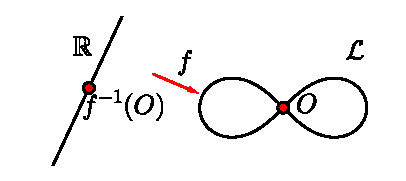
\includegraphics[scale = 0.75]{img/lemniscata}
			\caption{Ilustración del argumento intuitivo.}
			\label{cont_img_lemins}
		\end{figure}
		
		\item \begin{figure}[h!]
			\centering
			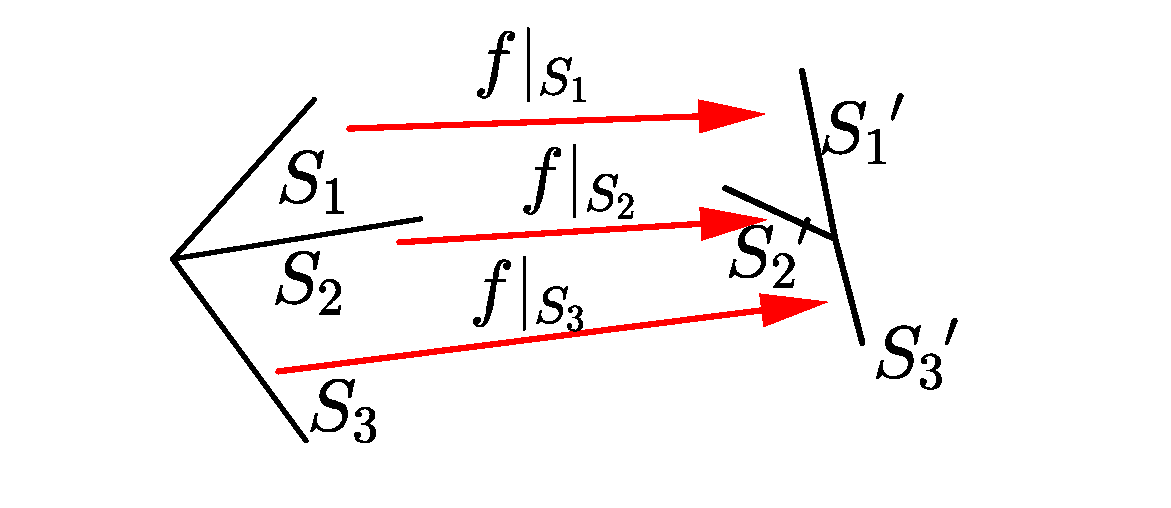
\includegraphics[scale = 0.3]{img/segmentos}
			\caption{Ilustración del homeomorfismo.}
			\label{cont_img_sementos}
		\end{figure}
		
		Sea $\X$ un conjunto de $3$ segmentos cualesquiera de $\R^2$ que comparten un punto extremo e $\Y$ otro conjunto de $3$ segmentos arbitrarios que comparten otro punto extremo (véase la ilustración \ref{cont_img_sementos}). Si equipamos a ambos conjuntos con la topología relativa inducida por la topología usual de $\R^2$, entonces son homeomorfos.
		
		En efecto, tomando el recubrimiento por cerrados de $\X$ compuesto por cada uno de los segmentos y definiendo un homeomorfismo $f$ que a cada segmento (cerrado del recubrimiento de $\X$) le haga corresponder otro segmento de $\Y$ (sin repetir). Tenemos, por la proposición \ref{cont_prop_caracterizacion} que $\X$ e $\Y$ son homeomorfos (así de paso vemos que las proposiciones sirven para algo).
		
		Dicho homeomorfismo $f$ será la \tbi{interpolación lineal} que definimos como
		\begin{equation}
		\label{interpolacion}
			\begin{array}{cc}
			f_{ab}:&[0,1]\to\R^2\\
			& t\mapsto ta+(1-t)b
			\end{array}
		\end{equation}
		Que es un homeomorfismo (¡compruébese!) que transforma el intervalo $[0,1]$ en el segmento de $\R^2$ determinado por los puntos $a,b\in\R^2$, al que denotamos por $[a,b]$ con cierto abuso de notación.
		
		Para conseguir un homeomorfismo entre dos segmentos $[a,b]$ y $[c,d]$ cualesquiera basta seguir el siguiente diagrama.
		\[\xymatrix{[0,1]\ar[r]^{f_{ab}}\ar[d]_{f_{cd}}&[a,b]\\
			[c,d]\ar[ru]_{f_{ab}\circ f^{-1}_{cd}}
			}\]
	\end{enumerate}
	Con esto ya tenemos suficiente artillería para resolver gran cantidad de problemas.
\end{exa}

Una vez definido el concepto de homeomorfismo y vista a través de los ejemplos su gran fuerza, vamos a pasar al concepto de homeomorfismo local, el cual, a pesar de ser una relación más débil que la que proporciona el homeomorfismo, también será muy utilizado.

\begin{defi}[Homeomorfismo local]
	\label{cont_def_homeomorfismoLocal}
	Sea $f:X\rightarrow Y$ aplicación entre espacios topológicos y $x_0\in X$. Se dice que $f$ es \tbi[homeomorfismo!local]{homeomorfismo local} en $x_0$ si $x_0$ tiene un entorno abierto $U_{x_0}$ tal que $f(U_{x_0})$ es entorno abierto de $f(x_0)$ en $Y$ y se tiene que $f|_{U_{x_0}}:U_{x_0}\rightarrow f(U_{x_0})$ es homeomorfismo.
\end{defi}

De esta definición se desprende que todo un homeomorfismo entre dos espacios es en un homeomorfismo local en todos sus puntos. Este resultado resulta evidente, pero su contrarreciproco (no homeomorfo local implica no homeomorfo) nos puede resultar enormemente útil ya que es mucho más sencillo estudiar  el homeomorfismo local al global.

Vemos ahora, a modo de ejemplo que la esfera $\esfera^2:=\{x\in\R^3\midc\norm{x}=1\}$ es localmente homeomorfa al plano $\R^2$.

\begin{exa}[Esfera y plano]
	\label{cont_exa_homeomorfismoLocal}
	Vamos a contruir un homeomorfismo local entre la esfera y el plano.
	
	Resulta de interés destacar que no es necesario que la aplicación sea la misma en todo el espacio, sino que podemos tomar una distinta para cada punto del espacio.
	
	En efecto, sea $p:=(x_0,y_0,z_0)\in\esfera^2$ con $z_0\not=0$, entonces, dado un entorno abierto de $p$ que no corta al ecuador de la esfera y queda contenido en el hemisferio de $p$, definimos la aplicación
	\[\begin{array}{cc}
	f(x,y,z):=(x,y) \qquad& f^{-1}(x,y):=(x,y,\frac{z_0}{\abs{z_0}}\sqrt{1-x^2-y^2})
	\end{array}\]
	que es homeomorfismo local (¡compruébese!).
	
	Análogamente, si tomamos un $p':=(x_1,y_1,0)\in\esfera^2$ con $x_1>0$, dado un entorno abierto de $p'$ con todos los puntos con primera coordenada positiva definimos el siguiente homeomorfismo local (¡compruébese!)
	\[\begin{array}{cc}
	f(x,y,z):=(y,z) \qquad& f^{-1}(y,z):=(\sqrt{1-y^2-z^2},y,z)
	\end{array}\]
	Nótese que aún quedan puntos de la esfera por tratar (se dejan como ejercicio).
\end{exa}

Una vez vistas ambas definiciones pasamos a ver una serie de propiedades y observaciones propias de los homeomorfismos (globales), pero que también nos valdrán para la restricción homeomorfa de los locales (dado que en ella por definición la aplicación es homeomorfa).
\label{etop_obs_homeomorfismo}
\begin{obs}[Propiedades de los homeomorfismos]\
	\begin{enumerate}
		\item 
		Sea $f:X\rightarrow Y$ aplicación biyectiva.
		
		Que $f$ sea continua es equivalente a que si $U\in Y$ es abierto, $f^{-1}(U)$ también lo será. Del mismo modo, es equivalente a que si $F\in Y$ es cerrado, $f^{-1}(F)$ también lo será.
		
		Igualmente, que $f^{-1}$ sea continua es equivalente a que si $F\in X$ es cerrado, entonces $f(F)$ es cerrado, asimismo si $U\in X$ es abierto, $f(U)$ también lo será.
		
		Vemos como si se verifican ambas (la continuidad de $f$ y de su inversa) será homeomorfismo, de modo que $f$ es homeomorfismo si y solo si es continua, biyectiva y transforma abiertos en abiertos por imágenes directas.
		
		\item
		Una aplicación $f$ no necesariamente biyectiva se dice \tbi[aplicación!abierta]{abierta} cuando la imagen de abiertos es un abierto (es decir, cuando $f(U)$ es abierta si $U$ es abierto).
		
		Análogamente, una aplicación $f$ no necesariamente biyectiva se llama \tbi[aplicación!cerrada]{cerrada} cuando la imagen de cerrados es un cerrado (es decir, cuando $f(F)$ es cerrado si $F$ es cerrado).
		
		Dejamos como ejercicio al lector ver que si una es aplicación no es abierta no tiene por qué ser cerrada (y viceversa) y que si una aplicación es abierta y cerrada no tiene por qué ser biyectiva.\qedhere
		\end{enumerate}
\end{obs}

	%Para este capítulo se usará la abreviatura "const".
\chapter{Construcciones de espacios}
\label{const}

\section{Imágenes inversas}

Esta sección se centrará en dar solución al siguiente problema. Dado un espacio topológico $(\mathcal{X},\T)$, un conjunto $\mathcal{Y}$ y una aplicación $f$ que nace en $\mathcal{Y}$ y muere en $(\mathcal{X},\T)$, queremos dotar a $\mathcal{Y}$ de una topología que haga que $f$ sea continua. Evidentemente, una elección fácil para que esto ocurra es escoger la topología discreta, puesto que es la que cuenta con más abiertos y, por lo tanto, para todo abierto $U'$ de $\mathcal{X}$ entonces $f^{-1}(U')$ es abierto en $\mathcal{Y}$, lo que implica que $f$ sea continua. Sin embargo, este caso no es realmente interesante y lo difícil del problema será encontrar la topología menos fina para que $f$ sea continua.

La solución a este problema es la topología $f^{-1}(\T)$, definida como 

\[f^{-1}(\T)=\{f^{-1}(U):U\in \T\}\]

La comprobación de que verdaderamente es una topología se desprende de las propiedades de la función inversa aplicada a conjuntos. Por otro lado, es la menos fina que implica que $f$ sea continua por construcción, luego cualquier otra topología con estas características contiene a esta. Finalmente, se tiene que es única. En efecto, si tenemos que $\T$ y $\T$ cumplen que son las menos finas por construcción, entonces se tiene que $\T\subset \T'$ y $\T'\subset \T$, luego son iguales.

Una vez resuelta esta cuestión, es hora de profundizar un poco más. Tomemos otro espacio topológico $(\mathcal{Z},\T')$ y consideremos una función $g$ que nace en este y muere en $Y$. El problema que se nos plantea ahora es determinar qué aplicaciones $g$ son continuas. Nótese que con esta distribución también podemos definir la composición $f\circ g$, quedando el siguiente diagrama:

\begin{equation*}
\xymatrix{
	&\mathcal{Y} \ar[r]^f
	&(\mathcal{X},\T) \\
	&(\mathcal{Z},\T') \ar@{-->}[ru]_{f\circ g} \ar[u]^g}
\end{equation*}

En primer lugar, observemos que como $f$ es continua por definición del problema anterior, que $g$ sea continua implica que la composición $f\circ g$ también lo sea. Sin embargo, la otra implicación (si $f\circ g$ es continua entonces $g$ es continua) también es cierta como veremos a continuación. Esto es realmente interesante, puesto que la topología que haya en $\mathcal{Y}$ no es relevante si nuestro estudio se centra en la relación de $(\mathcal{X},\T')$ y $(X,\T)$.

Veamos que efectivamente se cumple esta implicación. En efecto, consideremos un abierto $W\subset f^{-1}(U)$ y verifiquemos que $g^{-1}(W)\subset \T'$. Por su definición, $W$ es un abierto de $f^{-1}(U)$ con $U\subset \T$ y, como $f\circ g$ es continua, entonces $(f\circ g)^{-1}(U)\subset \T'$. Pero se tiene que $f\circ g)^{-1}(U)=g^{-1}[f^{-1}(U)]\equiv g^{-1}(W)$, luego $g^{-1}(W)\subset \T'$.

Una consecuencia directa que se desprende de esto es que la topología imagen inversa $f^{-1}(\T)$ es la topología en $\mathcal{Y}$ que cumple la equivalencia anterior. En efecto, supongamos que una topología $\T_\mathcal{Y}$ lo cumple y veamos que coincide con la topología imagen inversa. Para ello, consideremos el siguiente diagrama

\begin{equation*}
\xymatrix{
	&(\mathcal{Y},\T_{\mathcal{Y}}) \ar[r]^f
	&(\mathcal{X},\T) \\
	&(\mathcal{Y},\T_{\mathcal{Y}}) \ar@{-->}[ru]_f \ar[u]^{\text{id}}}
\end{equation*}

Sabemos que la identidad de un espacio en sí mismo es una aplicación continua. De este modo, al ser esta continua, tenemos por lo anterior que $f$ es continua. En consecuencia, $\T_{\mathcal{Y}}$ hace que $f$ sea continua y, por tanto, $f^{-1}(\T)\subset \T_{\mathcal{Y}}$. Ya tenemos demostrada una inclusión.

Consideremos ahora el diagrama 

\begin{equation*}
\xymatrix{
	&(\mathcal{Y},\T_{\mathcal{Y}}) \ar[r]^f
	&(\mathcal{X},\T) \\
	&(\mathcal{Y},f^{-1}(\T)) \ar@{-->}[ru]_f \ar[u]^{\text{id}}}
\end{equation*}

Ahora, sabemos que $f$ es continua por lo visto en el primer problema. Además, como la diagonal es continua, entonces la vertical es continua, luego $\T_{\mathcal{Y}} \subset f^{-1}(\T)$.

\begin{obs}[Inyectividad]
	
	(1) Supongamos que dos puntos $y_1$ e $y_2$ terminan en el mismo punto tras ser evaluados en una aplicación (lo que quiere decir que esta no es inyectiva). Los abiertos $U$ que contienen a la imagen de los dos puntos mencionados $x$ (que es la misma) cumplen que $f^{-1}(U)$ contiene a $y_1$ e $y_2$, luego estos dos puntos resultan ser topológicamente indistinguibles. Por ello, este tipo de aplicaciones no presentan mucho interés puesto que no es posible conocer con certeza ciertas propiedades.
	
	(2) El caso verdaderamente interesante ocurre cuando $f$ es inyectiva. En este caso, si se considera el subespacio $(f(\mathcal{Y}),\left.\T\right|_{f(\mathcal{Y})}) \subset (\mathcal{X},\T)$, entonces $f$ es biyectiva:
	
	\[(\mathcal{Y},f^{-1}(U)) \xrightarrow{f} (f(\mathcal{Y}),\left.\T\right|_{f(\mathcal{Y})}) \subset (\mathcal{X},\T).\]
	
	Además, la aplicación es continua puesto que, dado $W$ un abierto de $f(\mathcal{Y})$, entonces $W=\mathcal{Y}\cap f(U)$ para cierto abierto $U\in \T$. Esto implica que
	
	\[f^{-1}(W)=f^{-1}(U\cap f(\mathcal{Y}))=f^{-1}(U)\cap \mathcal{Y}=f^{-1}(U),\]
	
	que es abierto de $\mathcal{Y}$ por la definición de topología que hemos tomado. Sin embargo, esto no termina aquí, ya que $f$ es abierta. En efecto, dado un abierto $W\subset \mathcal{Y}$, entonces existe un abierto $U\subset \T$ de modo que $W=f^{-1}(U)$. De este modo, 
	
	\[f(W)=f(f^{-1}(U))\cap f(\mathcal{Y})=(U)\cap f(\mathcal{Y})=f^{-1}(U),\]
	
	que es un abierto de $f(\mathcal{Y})$ (la segunda igualdad se deduce de que $f$ es inyectiva). Por tanto, al ser $f$ continua y abierta, es homeomorfismo. Esto es sorprendente, ya que una aplicación inyectiva de $\mathcal{Y}$ en $\mathcal{X}$ es homeomorfismo de $\mathcal{Y}$ en $f(\mathcal{Y})$. De aquí se puede definir el concepto de inmersión o embebimiento si $f$ es inyectiva y se tiene que 
	
	\[f:(\mathcal{Y},f^{-1}(\T)) \to (\mathcal{X},\T)\qedhere\]
	
\end{obs}

\section{Imágenes directas}

Después de haber realizado todo el desarrollo anterior, una posibilidad que se nos plantea es dualizar las cuestiones que nos han ido apareciendo. Coloquialmente, podríamos decir que vamos a cambiarle el sentido a todo.

Así pues, consideremos un espacio topológico $(\mathcal{X},\T)$, un conjunto $\mathcal{Y}$ y una aplicación $f$ que nace en $(\mathcal{X},\T)$ y muere en $\mathcal{Y}$. El problema ahora consiste en dotar a $\mathcal{Y}$ de una topología que haga que $f$ sea continua. La solución más sencilla sería elegir la topología trivial, puesto que sus únicos abiertos son el vacío y el total y siempre se cumpliría que para cada $U'$ abierto de $\mathcal{Y}$ entonces la imagen inversa de este es un abierto del espacio de partida. No obstante, es interesante encontrar la topología más fina que cumpla esto, y esta es 

\[f(\T)=\{U: f^{-1}(U)\in \T\}\]

Evidentemente, se trata de una topología y es la más fina que permite que $f$ sea continua ya que si se añade algún abierto más deja de serlo. Por último, realizando un razonamiento por doble inclusión al análogo en imágenes inversas, se puede ver que es única.

Continuando con la misma argumentación, veamos cuando una función $g$ que parta de $\mathcal{Y}$ es continua

\begin{equation}
\label{cont_propiedad_universal_top_imagen}
\xymatrix{
	(\mathcal{X},\T) \ar[r]^f \ar@{-->}[rd]_{g\circ f} &
	\mathcal{Y} \ar[d]^g & \\
	&(\mathcal{Z},\T')}
\end{equation}

Trabajando igual que en el caso anterior, se llega a que $g$ es continua si y solo si $g\circ f$ es continua (para ello, basta ver que si $W\subset \T'$ entonces $g^{-1}(W)\subset f(\T)$) y que $f(\T)$ es la topología en $\mathcal{Y}$ que cumple esta doble implicación.

\begin{obs}[Sobreyectividad]
	
	(1) Supongamos que $f$ no es sobreyectiva y tomemos un punto $y\notin f(\mathcal{X})$. Entonces $f^{-1}(\mathcal{Y})$ es el vacío, pero como el vacío es abierto llegamos a que el punto es abierto, luego $f(\left.\T\right|_{\mathcal{Y}\backslash f(\mathcal{X})})$ coincide con la topología discreta. Sin embargo, la imagen inversa de $\mathcal{Y}\backslash f(\mathcal{X})$ es vacía y es abierta en la imagen. Además, como $f(\mathcal{X})$ es el complementario de $\mathcal{Y}\backslash f(\mathcal{X})$, entonces $f(\mathcal{X})$ es cerrado. No obstante, $f(\mathcal{X})$ coincide con el total, luego también es un abierto. 
	
\end{obs}

Ahora que hemos visto que el caso interesante es que $f$ sea sobreyectiva, consideramos el siguiente diagrama:
\[\xymatrix{
	(\X,\T) \ar[r]^{f} \ar[d]_{p} &
	(\mc{Y}, f\T) \\
	\X/\mathord{\sim}  \ar[ru]_{\bar{f}}
}\]
donde la relación de equivalencia verifica $x\sim y\iff f(x)=f(y)$. Aquí, $p$ es simplemente la aplicación que manda $x\in\X$ a su clase de equivalencia, y consideramos $\bar{f}$ de forma que verifique que $f=\bar{f}\circ p$.

% Esto no lo nombró él en clase pero lo he encontrado por ahí y es cómodo
Decimos que una aplicación $f$ que verifica que si $x\sim y$ entonces $f(x)=f(y)$ respeta la relación de equivalencia $\mathord{\sim}$. Nótese que no se exige la equivalencia, solo la implicación.

Como hemos definido la relación de equivalencia como la que verifica $x\sim y\iff f(x)=f(y)$, tenemos que $\bar{f}$ es una biyección. Además, se puede comprobar que si existe $\bar{f}$ tal que $f=\bar{f}\circ p$, entonces $f$ respeta la relación de equivalencia $\mathord{\sim}$.

Ahora, vamos a definir la topología cociente para $\X/\mathord{\sim}$. Buscamos una topología que verifique que la aplicación $p$ es continua y que existe una aplicación continua $\bar{f}$ que respete la relación de equivalencia $\mathord{\sim}$ y que verifique que $f=\bar{f}\circ p$.

\begin{defi}[Topología cociente]
	Definimos la \tbitop[$\T/\mathord{\sim}$]{cociente} en las condiciones anteriores como:
	\[\T/\mathord{\sim} = \{V\midc p^{-1}(V)\in\T\}\]
	es decir, la topología cociente es la topología imagen por $p$.
\end{defi}

Está claro que se verifican nuestros requisitos. Por un lado, $p$ es trivialmente continua (pues la topología imagen por $p$ es precisamente la que verifica esto). Por otro lado, por ser una topología imagen se verifica directamente la continuidad de $\bar{f}$.

\begin{prop}
	En las condiciones de la construcción (cuando la relación $\sim$ está definida como $x\sim y\iff f(x)=f(y)$), $\bar{f}$ es homeomorfismo.
	
	\begin{proof}
		Ya hemos visto que $\bar{f}$ es biyectivo cuando la relación de equivalencia verifica $x\sim y\iff f(x)=f(y)$; y que es continuo en el sentido en el que lo hemos definido. Para ver la continuidad en el otro sentido, basta con ver que $\bar{f}$ es abierta.
		
		En efecto, $U\in \X/\mathord{\sim}$ abierto $\iff p^{-1}(U)$ es abierto en $\X$. Pero tenemos que $p^{-1}(U)=f^{-1}(f(S))$, porque:
		\[x\in p^{-1}(U)\iff p(x)\in S\stackrel{\bar{f}\text{ biy.}}{\iff}\bar{f}(p(x))\in \bar{f}(U)\iff f(x)\in\bar{f}(U)\iff x\in f^{-1}(\bar{f}(U))\]
		
		Entonces, como $f(\T)$ es la topología en $\mc{Y}$, $f^{-1}(f(U))$ es abierto en $\X\iff \bar{f}(U)$ es abierto en $\mc{Y}$, pero ya hemos visto que $f^{-1}(f(U))$ es abierto, porque es $p^{-1}(U)$.
	\end{proof}
\end{prop}

Por otro lado, está claro que todos los abiertos de $\T/\mathord{\sim}$ son imágenes por $p$ de abiertos de $\T$ (pero no todas las imágenes de abiertos tienen que estar necesariamente en $\T$). Entonces, definimos:

\begin{defi}[Conjunto saturado]
	En las condiciones anteriores, decimos que $W\in\T$ es \tbi[conjunto!saturado]{saturado} si $W=p^{-1}(p(W))$. Es equivalente decir que $[x]\cap W\neq\emptyset\implies [x]\subset W$, o que $x\in W,y\sim x\implies y\in W$.
\end{defi}

Gracias a esta definición, podemos reescribir la topología cociente como:
\[\T/\mathord{\sim} = \{p(W)\midc W\in\T\text{, } W\text{ saturado}\}\]

Además, vamos a dar un nombre a las funciones que envían $X$ en un espacio homeomorfo a un cociente:

\begin{defi}[Identificación]
	Una \tbi{identificación} es una aplicación $f:(X,\T)\to (\mc{Y},\T')$ sobreyectiva que verifica que $\T'$ es la topología imagen por $f$ $f(\T)$.
\end{defi}

La aplicación $f$ con la que hemos estado trabajando es, entonces, una identificación. El hecho de que la topología de $\mc{Y}$ sea la imagen significa que una identificación es continua.

Las identificaciones se llaman a veces en la literatura aplicaciones cociente\index[general]{aplicación!cociente}. Esto está ligado con su utilidad: las identificaciones son aquellas que inducen una relación de equivalencia $\sim$ de forma que podemos desarrollar toda la construcción anterior. De esta forma, nos ``regalan'' un espacio homeomorfo a $\mc{Y}$ que a menudo es más simple y más fácil de entender que él. Este propósito quedará más claro en los ejemplos posteriores.

Para comprobar si una aplicación es una identificación, podemos usar la siguiente proposición:

\begin{prop}[Condiciones suficientes de identificación]
	Sea $f:\X\to\mc{Y}$ una aplicación. Si se verifica alguna de las siguientes condiciones, $f$ es una identificación:
	\begin{enumerate}
		\item $f$ es una aplicación continua abierta.
		\item $f$ es una aplicación continua cerrada.
	\end{enumerate}
\end{prop}

Nótese que puede haber identificaciones que no verifiquen ninguna de las condiciones anteriores. Además, como no se exige que las identificaciones sean biyectivas, las dos condiciones anteriores no son equivalentes.

Toda esta construcción abstracta debe servirnos para formalizar todo el concepto de cociente de un espacio. Esta es quizá la idea más importante que se va a ver en toda la asignatura, y es excepcionalmente útil para construir una gigantesca variedad de homeomorfismos y encontrar objetos simples homeomorfos a otros mucho más complejos.



\begin{exa}[Circunferencia unidad]
	Definimos la aplicación:
	\[\begin{split}
	\R&\to\esfera^1 \\
	t&\mapsto e^{2\pi it}=(\cos 2\pi t,\sen 2\pi t)
	\end{split}\]
	y consideramos la relación de equivalencia $s\sim t\iff e^{2\pi is}=e^{2\pi it}\iff s-t\in\Z$. Vamos a ver que la circunferencia unidad $\esfera^1$ es homeomorfa a $\R/\mathord{\sim}$.
	
	Nos queda, pues, el siguiente esquema:
	\[\xymatrix{
		\R \ar[r] \ar[d] &
		\esfera^1 \\
		\R/\mathord{\sim}  \ar@{<->}[ru]
	}\]
	y está claro que la aplicación que manda $f$ a $\esfera^1$ es una identificación, pues es sobreyectiva, continua y homeomorfismo local, luego es abierta.
	
	Ahora, nótese que considerando $[0,1]\subset\R$ podemos tomar las restricciones correspondientes con el siguiente esquema:
	\[\xymatrix @C=0.5pc @R=0.5pc @L=-0.2pc {
		& \R \ar[rr] \ar[dd] & &
		\esfera^1 \\
		[0,1] \ar@{}[ur]^*[@]{\subset} \ar[dr] \\
		& \R/\mathord{\sim}  \ar@{<->}[rruu]
	}\]
	y llegar a otra identificación. Ahora la relación de equivalencia asociada es simplemente aquella en la que $1\sim 0$ y todos los demás puntos son solamente equivalentes a sí mismos.
\end{exa}

Esta posibilidad de encontrar, a veces, un cociente más simple que tiene la misma topología nos motiva a definir:

\begin{defi}[Dominio fundamental]
	En una construcción como la anterior, llamamos \tbi{dominio fundamental} a la región cerrada más pequeña posible con un representante de cada clase de equivalencia. Según la situación, a veces se exigen también otras propiedades como compacidad.
\end{defi}

\begin{exa}
	Ahora, vamos a considerar el toro de revolución que vive en $\R^3$, cuya parametrización es conocida:
	\[\begin{split}
	x&=(a\cos(\theta)+b)\cos(\phi),\\
	y&=(a\cos(\theta)+b)\sin(\phi),\\
	z&=a\sin(\theta).
	\end{split}\]
	
	Como vemos en la imagen, se trata de una figura generada por revolución de una circunferencia en torno a un eje.
	
	\begin{figure}[h!]
		\centering
		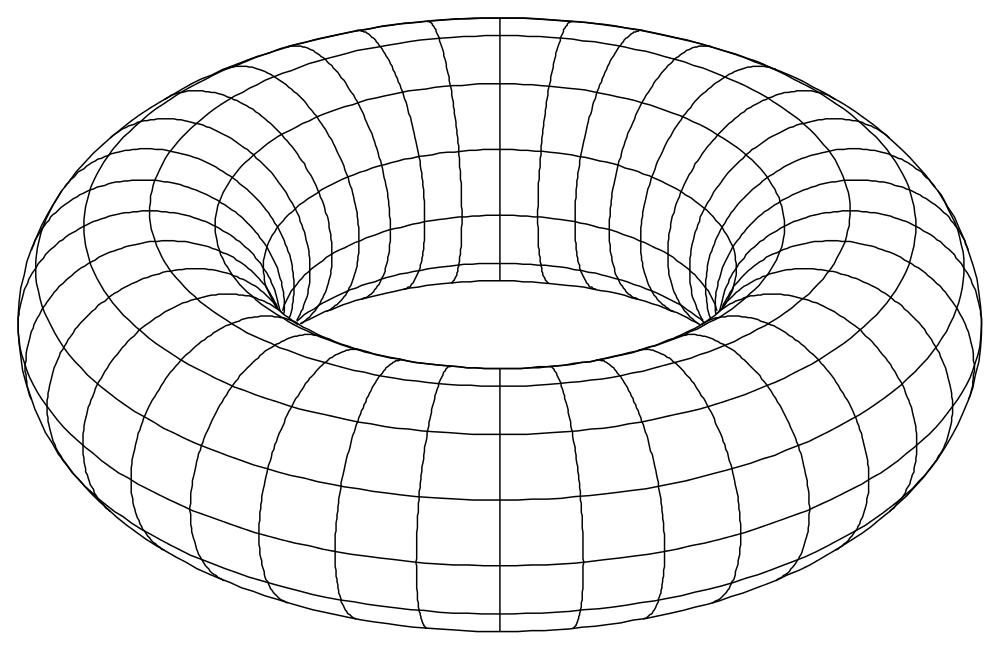
\includegraphics[scale = 0.15]{img/toro}
	\end{figure}
	
	Vamos a hacer pues una construcción similar a la ya vista para la circunferencia unidad. Nos queda un esquema del siguiente tipo:
	
	\[\xymatrix @C=0.5pc @R=0.5pc @L=-0.2pc {
		& \R^2\ar[rr] \ar[dd] & &
		\toro^2\subset\R^3 \\
		[0,2\pi]^2 \ar@{}[ur]^*[@]{\subset} \ar[dr] \\
		& \R^2/\mathord{\sim}  \ar@{<->}[rruu]
	}\]
	
	En este caso, la relación de equivalencia está definida como:
	\[(x,y)\sim (x',y')\iff x-x'\in\Z,\;y-y'\in\Z\]
	y como dominio fundamental encontramos el cuadrado $[0,2\pi]^2$. 
	
	A menudo, los dominios fundamentales se representan con esquemas llamados \tbi[polígono fundamental]{polígonos fundamentales}. La forma de entenderlos es que la relación de equivalencia ``pega'' los puntos de $A$ y de $B$ en el sentido que indican las flechas, como vemos en el ejemplo siguiente, que representa el toro que acabamos de describir:
	
	% Copiado de https://en.wikipedia.org/wiki/Fundamental_polygon . Querría hacer uno yo pero no ha dado tiempo.
	\begin{figure}[h!]
		\centering
		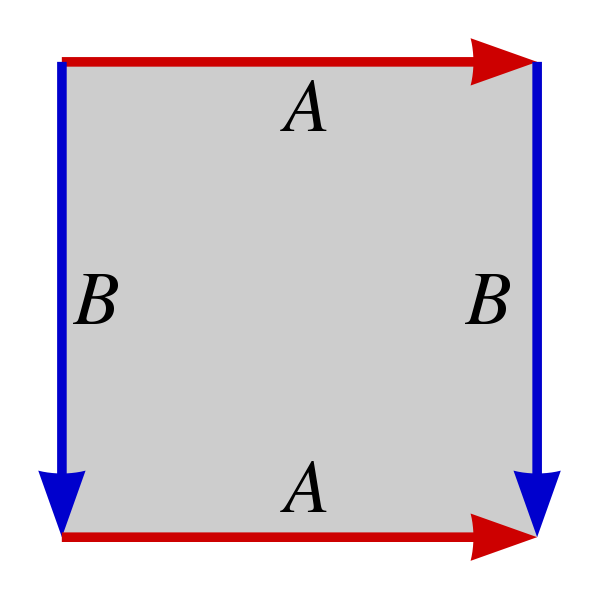
\includegraphics[scale = 0.1]{img/pol_fund_toro}
	\end{figure}
\end{exa}

En el siguiente ejemplo, vamos a ver varios homeomorfismos cociente importantes pero sin entrar en tantos detalles como en los ejemplos previos. Para familiarizarnos íntimamente con el espacio cociente, es un buen ejercicio mental tratar de visualizar cómo podemos deformar un objeto del ejemplo siguiente para transformarlo en otro homeomorfo. Al fin y al cabo, la homeomorfia, intuitivamente, es poder deformar sin romper, y los cocientes formalizan la noción de ``pegar'' puntos.

\begin{exa} \
	\begin{enumerate}
		\item La esfera $\esfera^2$ se puede identificar con el disco unidad si la relación de equivalencia es la que hace que todos los puntos del borde estén relacionados entre sí y los demás, solo con sí mismos. De la misma forma, la podemos identificar con dos discos donde la relación de equivalencia ``pega'' los bordes. Por último, una esfera tiene como polígono fundamental:
		
		\begin{figure}[h!]
			\centering
			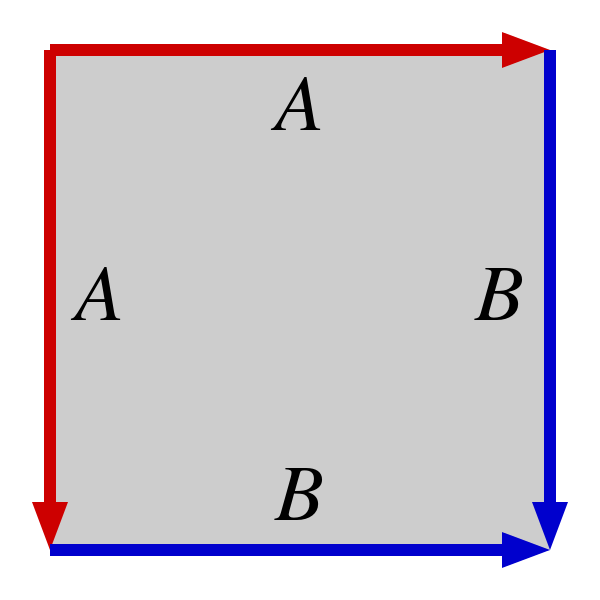
\includegraphics[scale = 0.1]{img/pol_fund_esfera}
		\end{figure}
		
		\item Podemos identificar el plano proyectivo real $\proy^2$ con un disco y una esfera donde la relación de equivalencia ``pega'' los bordes. También podemos identificarlo con una semiesfera en la que cada punto del borde es equivalente a su antípoda, o con una esfera completa en la que dos puntos están relacionados si y solo si son antipodales. Además, el polígono fundamental del plano proyectivo real sería:
		
		\begin{figure}[h!]
			\centering
			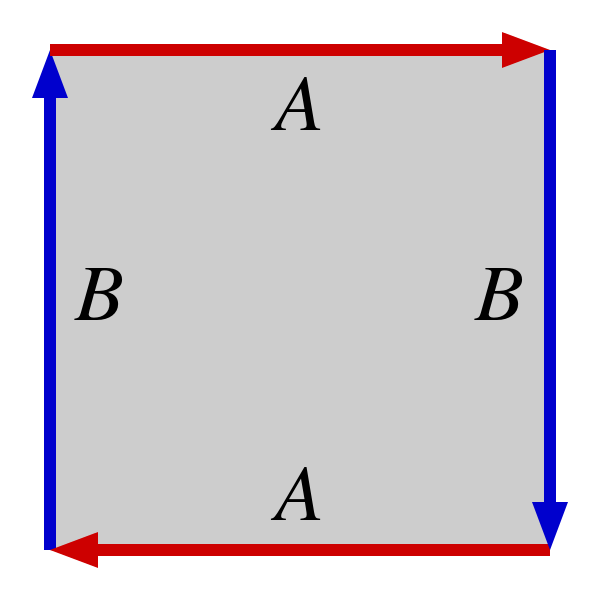
\includegraphics[scale = 0.1]{img/pol_fund_plano_proy}
		\end{figure}
		
		\item Vamos a ver otros dos polígonos fundamentales más. El de la banda de Möbius sería:
		
		\begin{figure}[h!]
			\centering
			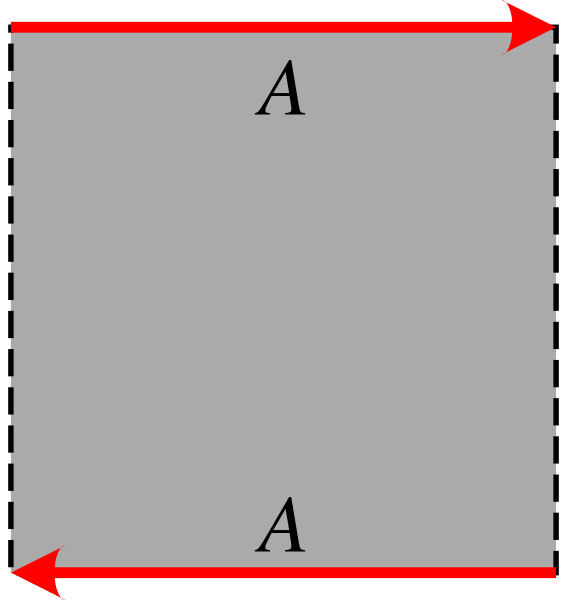
\includegraphics[scale = 0.09]{img/pol_fund_mobius}
		\end{figure}
		
		Nótese que en este caso hay un lado que no se pegaría, que corresponde al borde de la banda de Möbius. 
		\newpage
		Por otro lado, el de la botella de Klein sería:
		\begin{figure}[h!]
			\centering
			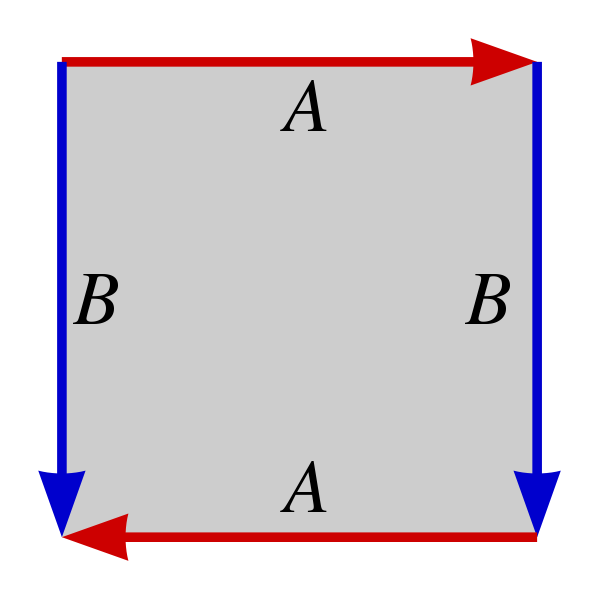
\includegraphics[scale = 0.1]{img/pol_fund_botella_klein}
		\end{figure}
	\end{enumerate}
\end{exa}

\section{Producto de espacios topológicos}
Una vez visto el caso del espacio cociente, pasamos ahora a realizar un desarrollo similar para otras construcciones como son los productos y sumas de espacios topológicos. Se va a realizar un procedimiento análogo en el desarrollo de las mismas al de la anterior sección.

Sean $(X_{i },\T_{i})^{1\le i\le r}$ espacios topológicos y sea $Y=\prod_i X_i$. Tomamos entonces 
\begin{equation}
Y=\prod_i X_i \stackrel{p_i^r}{\longrightarrow}(X_i,\T_i)
\end{equation}
Lo que buscamos en la construcción del espacio producto es de dotar a $Y$ de la topología $\T$ más fina haga continuas todas las aplicaciones $p_i^r$ para $1\le i\le r$. A dichas  $p_i^r$ las conoceremos a partir de ahora como \tbi{proyecciones}.

De este modo, como queremos que $(p_i^r)^{-1}$ sea continua  tenemos que para todo abierto $U_i\in \T_i$ deberá verificarse que $(p_i^r)^{-1}(U_i)=X_1\times\cdots\times U_i\times\cdots X_r$ (todos son los totales excepto en el caso de $X_i$) sea abierto. Es decir, que se cumpla $X_1\times\cdots\times U_i \times\cdots X_r\in \T$

Por lo tanto, vemos que por ser topología ha de verificarse que $(p_i^r)^{-1}(U_i)\cap (p_j^r)^{-1}(U_j)= \cdots\times U_i \times\cdots\times U_j\times \cdots$ sea parte de ella (intersección de abiertos).

Si tomamos ahora $ \{ U_1\times\cdots\times U_r : U_i\in \T_i \}$ veamos que es una base de la topología que pretendemos construir. Esto va a resultar evidente, ya que tan solo debemos comprobar para demostrarlo que al intersecar dos elementos cualesquiera de la base nos queda otro elemento de la base. 

Como dados $U_1\times\cdots\times U_r$ y $V-1\times\cdots\times V_r$ elementos de la base su intersección es $(U_1\cap V_1)\times\cdots\times (U_r\cap V_r)$ y como $(U_i\cap V_i)\in \T_i$, afirmamos que forma parte de la base por la definición de la misma.

Así, una vez que tenemos la base que va a caracterizar nuestra topología producto podemos afirmar que esta viene dada por $\T=\prod_i \T_i$.

\begin{defi}[Topología producto]
	Sean $(X_{i },\T_{i})^{1\le i\le r}$ espacios topológicos y sea $Y=\prod_i X_i$. Entonces se conoce como \tbi{topología producto} a la topología $\T$ de $Y$ que viene dada por la base $ \{ U_1\times\cdots\times U_r : U_i\in \T_i \}$ (es decir, el producto de las topologías).
\end{defi}
\begin{lem}[Propiedad Universal]
	En la siguiente situación,%añadir figura wiki
	
	Tenemos la siguiente \tbi{propiedad universal del producto} que caracteriza la continuidad de $f$ diciendo que esta será continua si y solo si  $f_i=p_i^r\circ f$ son continuas para todo $i$.
	
	\begin{proof}
		Vemos que si $f$ es continua, como $p_i^r$ son continuas, tenemos que $f_i$ también lo será al ser composición de estas.
		
		Por otro lado, tenemos que dado $W=\prod_iU_i$ abierto en $X$, tenemos que $f^{-1}(W)=\bigcap_i f_i^{-1}(U_i)$ será abierto dado que los $f_i^{-1}(U_i)$ son abiertos por ser $f$ continua. Así, como hemos probado que la imagen inversa de abiertos es abierta, tenemos que $f$ es continua.
	\end{proof}
\end{lem}

Veamos ahora una serie de proposiciones relacionadas con la topología producto, las cuales a pesar de resultar sencillas de comprobar nos proporcionan resultados interesantes.

\begin{prop}
	Las proyecciones son abiertas
	
	\begin{proof}
		Sea $W$ abierto en el espacio producto, veamos que $p_i^r(W)$ es abierto.
		
		Nos basta con comprobarlo con los abiertos de la base, es decir, para los elementos de la forma $ U_1\times\cdots\times U_r : U_i\in \T_i$.  Como  $p_i^r(U_1\times\cdots\times U_r)=U_i$ es abierto podemos concluir la demostración.
	\end{proof}
\end{prop}


\begin{prop}
	La aplicación $X:\longrightarrow\{a1\}\times\cdots\times X_i\times\cdots\times \{ar\}\in X_1\times\cdots\times X_r$ tal que $x\longrightarrow (a_1,\dots,a_r)$ es una inmersión.
	
	\begin{proof}
		Veamos primero como transforma la base de abiertos del inicial en la base del final.
		$U_i\longrightarrow\{a1\}\times\cdots\times U_i\times\cdots\times \{ar\}=\{a1\}\times\cdots\times X_i\times\cdots\times \{ar\}\cap(U_1\times\cdots\times U_r)$
		
		Como observamos esto se verifica y además la aplicación al serlo en los abiertos de las bases verifica ser biyectiva, continua y abierta por lo que se tratará de una inmersión.
	\end{proof}
\end{prop}

Ahora pasamos a ver si somos capaces de construir bases más sencillas para nuestra topología producto, es decir, conformadas por menos abiertos. Igualmente, veremos el modo de construcción de bases de entornos en el espacio producto. No vamos a probar que sean bases realmente en ninguno de los dos casos ya que en ambos casos va a resultar muy sencillo aplicando la caracterización de base, dejándose como ejercicio para el lector de cara al repaso de la misma.
\begin{enumerate}
	\item Dado el espacio producto $(\prod_iX_i,\prod_i\T_i)$ tenemos que $\B=\{W_i\times\cdots\times W_r:W_i\in \B_i$ base de $\T_i\}$ es base de entornos del mismo.
	\item Dado el espacio producto $(\prod_iX_i,\prod_i\T_i)$ y $(a_1,\dots,a_r)\in\prod_iX_i$ tenemos que $\V^{(a_1,\dots,a_r)}=\{V^{a_1}\times\cdots\times V^{a_r}:W_i\in \V^{a_i} \text{ base de entornos en } \T_i \}$ es base de entornos del mismo.
\end{enumerate}
	%Para este capítulo se usará la abreviatura "sep".
\chapter{Separación}

\section{Separación de puntos} 

La separación de puntos consiste en, dados dos puntos distintos, saber ``distinguirlos topológicamente'' (sea lo que sea eso). Presentamos algunas formas de entender el significado de la pedante expresión entrecomillada.
\begin{defi}[Axiomas de separación]
	\label{sep_defi_axiom}
Sea $(\X,\T)$ un espacio topológico.
\begin{itemize}
\item Se dice que $\X$ es \kolmogorov o \ti{\tb{Kolmogorov}} si para cada par de puntos existe un entorno de uno de los dos puntos (sin especificar cuál) que no contiene al otro. \indexg{Kolmogorov} \indexg{T0@\kolmogorov|see{Kolmogorov}}
\item $\X$ es \frechet o \ti{\tb{Fréchet}} si dados dos puntos $x$ e $y$, existe un entorno $\V_x$ de $x$ que no contiene a $y$ y también existe un entorno $\V_y$ de $y$ que no contiene a $x$. \indexg{Frechet@Fréchet} \indexg{T1@\frechet|see{Fréchet}}
\item Por último, se dice que $\X$ es \hausdorff o \ti{\tb{Hausdorff}} si dados $x,y\in\X$ existen un entorno $\V_x$ de $x$ y un entorno $\V_y$ de $y$ tales que son disjuntos. \indexg{Hausdorff} \indexg{T2@\hausdorff|see{Hausdorff}}
\end{itemize}
\end{defi}

\begin{obs}[Consecuencias inmediatas]
	De la definición \ref{sep_defi_axiom} se desprende que:
	\begin{enumerate}
		\item Todo espacio métrico es \hausdorff. En efecto, si consideramos dos puntos distintos $x$ e $y$, podemos tomar bolas centradas en cada uno de los puntos de radio menor que la mitad de la distancia que los separa. Compruébese que de este modo resolvemos el problema.
		\item Es claro que se da la cadena de implicaciones
			\hausdorff $\ra$ \frechet $\ra$ \kolmogorov.\qedhere
	\end{enumerate}  
\end{obs}

\section{Caracterizaciones}

En esta subsección vamos a estudiar varios resultados útiles que se desprenden directamente de la definción \ref{sep_defi_axiom}.

Comencemos con una reformulación de lo que significa ser \frechet
\begin{prop}[Caracterización de \frechet]
	$\X$ es \frechet si y solo si sus puntos son cerrados.
\end{prop}
\begin{proof}Procedemos por doble implicación.
	\begin{enumerate}
		\item[\bla]Consideremos un par de puntos cualquiera $x,y\in \X$. Como $\{x\}$ es cerrado, su complementario, $\U:=\X\backslash \{x\}$, es abierto, y, por tanto, entorno de todos sus puntos. Como $y\in\U$, tenemos un entorno de $y$ que no contiene a $x$. Para encontrar un entorno de $x$ que no contenga a $y$ basta intercambiar los papeles de $x$ e $y$.
		\item[\bra] Sea $x\in\X$, veamos que $\X\setminus \{x\}$ es abierto viendo que es entorno de todos sus puntos. En efecto, dado $y\in\X\setminus \{x\}$, como $\X$ es \frechet, hay un abierto de $y$ que no contiene a $x$, luego $\X\setminus \{x\}$, como $y$ es arbitrario hemos terminado.\qedhere
	\end{enumerate}		 
\end{proof}
Veamos a continuación una de las propiedades más importantes de los espacios \hausdorff.
\begin{theo}[Clausura del conjunto coincidente]
	Si $f,g:\X\to \Y$ son funciones continuas e $\Y$ es \hausdorff, entonces $\{f=g\}:=\{x\in\X\midc f(x)=g(x)\}\subset\X$ es cerrado. 
\end{theo}
\begin{proof}
	Procederemos demostrando que el conjunto $\{f\neq g\}$ es abierto, para lo cual usaremos (¡oh, sorpresa!) que es entorno de todos sus puntos.
	
	Dado $x\in \{f\neq g\}$, al ser $\Y$ \hausdorff, existen entornos $\V_f$ de $f(x)$ y $\V_g$ de $g(x)$ disjuntos. 
	
	Como $f$ y $g$ son continuas, transforman entornos en entornos por imágenes inversas, por ende, tenemos que $W:=f^{-1}(\V_f)\cap g^{-1}(\V_g)$ es entorno de $x$ (por ser intersección de entornos).
	
	Veamos pues que $W$ está contenido en $\{f\neq g\}$. En efecto, si hubiera un $y\in W$ tal que $f(y)=g(y)=:z$, entonces, por definición de $\V_f$ y $\V_g$, $z\in \V_f\cap \V_g$, lo cual es imposible.
\end{proof}

En general el recíproco de este teorema no se da, no obstante, hay un caso particular en el que sí. Antes de ver la demostración de este hecho, estudiemos el caso particular, que tiene interés por sí mismo.
\begin{obs}[Proyecciones]
	\label{sep_obs_proyecciones}
	Consideremos el espacio producto $\X\times \X$ y las proyecciones $p_1$ y $p_2$.
	
	El resultado anterior nos da que $\{p_1=p_2\}$ es un conjunto cerrado. Nótese que dicho conjunto no es más que $\{(x,y)\in\X^2\midc x=y\}$.
	
	Interpretado geométricamente en el caso particular de $\R^2$, es la recta diagonal $y=x$.
\end{obs}
\begin{lem}[Recíproco]
	En las condiciones de la observación \ref{sep_obs_proyecciones}.
	
	Si $\{p_1 = p_2\}$ es cerrado entonces $\X$ es \hausdorff.
\end{lem}
\begin{proof}
	Sea un par de puntos arbitrarios $x,y\in\X$.
	
	Como $x\not= y$ es claro que $(x,y)\not\in\{p_1=p_2\}$ (abierto), luego habrá un abierto (que podemos tomar de la base sin pérdida de generalidad) tal que $(x,y)\in\U_1\times\U_2\subset\{p_1\not=p_2\}$.
	
	Además, $\U_1$ y $\U_2$ son disjuntos, ya que si hubiera un $z\in\U_1\cap\U_2$ entonces $(z,z)\in\U_1\times\U_2$, pero $(z,z)\in \{p_1=p_2\}$, lo cual entra en contradicción con que $\U_1\times\U_2\subset \{p_1\not=p_2\}$.
\end{proof}
\begin{cor}[Densos]
	\label{sep_cor_densos}
	Si $f,g:\X\to \Y$ son funciones continuas que coinciden en un conjunto denso en $\X$ e $\Y$ es \hausdorff entonces $f$ y $g$ son iguales. 
\end{cor}
\begin{proof}
	Sea $A\subset \X$ un conjunto denso, es decir, $\adher{A}=\X$. Por hipótesis, $A\subset \{f=g\}$.
	
	Como $\{f=g\}$ es cerrado, por ende, $\X=\adher{A}\subset \{f=g\}$, luego $\{f=g\}=\X$.
	\end{proof}
\begin{obs}[Teoremas de extensión de la continuidad]
	Sea $f$ una función continua. Tomemos como espacio topológico la adherencia del dominio de $f$.
	
	Si $f$ admite una extensión continua a la adherencia, por el corolario \ref{sep_cor_densos} esta es única, ya que si hubiera dos extensiones distintas estas coincidirían en un conjunto denso. 
\end{obs}
\section{Comportamiento topológico} 
A partir de ahora dedicaremos la última sección de cada capítulo a estudiar si la propiedad estudiada en el mismo es ``hereditaria'' a las diferentes construcciones que hemos visto. Es decir, subespacios, productos, cocientes y sumas. Como hay que dar un nombre a todo, nosotros a esto lo llamaremos estudiar el ``comportamiento topológico''.

Inauguramos esta tradición estudiando el comportamiento topológico de \hausdorff, \frechet y \kolmogorov.
\subsection{Comportamiento topológico de \hausdorff, \frechet y \kolmogorov}
Comenzamos estudiando el comportamiento respecto de los subespacios.
\begin{lem}[Subespacios]
	Si $\X$ es \hausdorff, entonces $A\subset\X$ es \hausdorff.
\end{lem}
\begin{proof}
	 Sean $x,y\in A$. Al pertenecer estos puntos también a $\X$, existen sendos entornos disjuntos $\V_x$ y $\V_y$ de $x$ e $y$ en $\X$ respectivamente. Tomando los correspondientes entornos relativos $\V^x \cap A$ y $\V^y \cap A$ se sigue el resultado.
\end{proof}
Pasamos a estudiar los cocientes, tenido en mente que la filosofía de ``pegar puntos'' es bastante dañina para que las propiedades se conserven (luego iremos buscando contraejemplos).
\begin{obs}[Cocientes]
	La propiedad de ser \hausdorff no se traspasa a los cocientes.
	
	Un contraejemplo sencillo se da con el espacio topológico $\R$ y su cociente $\R/\Q$, donde se ha ``cocientado'' por la relación de equivalencia que relaciona a cada punto consigo mismo y a todos los racionales entre sí (y se le ha equipado con la topología cociente, claro).
	
	La idea que uno debe tener en la cabeza es que colapsamos todos los racionales a un solo punto.
	
	La clave para darse cuenta de que $\R/\Q$ no es \hausdorff es que los abiertos de $\R/\Q$ son las proyecciones de los abiertos saturados de $\R$. Como en $\R$ todo abierto contiene algún racional (por ser los intervalos una base de $\R$), todos los abiertos saturados contienen a $\Q$.
	
	Por ende, $\class{\Q}\in\R/\Q$ es un punto denso ya que todo abierto del cociente lo contiene. Luego dados dos abiertos cualesquiera nunca son disjuntos (y por tanto no puede ser \hausdorff).
\end{obs}
\begin{lem}[Productos]
	Si $X_i$ es \hausdorff para todo $i\in\{1,\dots,r\}$, entonces $\prod_{i=1}^rX_i$ también es \hausdorff.
\end{lem}
\begin{proof}
	Dados $x_i,y_i\in X_i$ es claro que hay sendos entornos $U_i$ y $V_i$ de $x_i$ e $y_i$ respectivamente tales que $U_i\cap V_i=\emptyset$.
	
	Haciendo lo anterior para cada $i$ obtenemos dos puntos $x=(x_1,\dots,x_r)$, $y=(y_1,\dots,y_r)$ de los cuales (por construcción de la topología producto) tenemos dos entornos $\prod_{i=1}^rU_i$ y $\prod_{i=1}^rV_i$ que son disjuntos por el lema \ref{const_lem_cartesiano}.
\end{proof}
Lo mismo se hace para la suma.
\begin{lem}[Suma]
	La suma finita de espacios \hausdorff es \hausdorff
\end{lem}
\begin{proof}
	Usaremos que las inclusiones son inmersiones. Sean dos puntos $x,y\in\sum_{i=1}^rX_i$.
	
	Si están en el mismo estante, es decir $x,y\in \{i\}\times X_i$ para cierto $i$, entonces tomamos $(j_i)^{-1}(x)$ y $(j_i)^{-1}(y)$ (puntos distintos de $X_i$). Como $X_i$ es \hausdorff tomamos los abiertos correspondientes $U$ y $V$ disjuntos. Como $j_i$ es homeomorfismo los abiertos imagen también son disjuntos.
	
	Si están en estantes distintos basta coger como abiertos disjuntos $\{i\}\times X_i$ y $\{j\}\times\{X_j\}$
\end{proof}
De manera totalmente análoga puede demostrarse que la propiedad de ser un espacio \kolmogorov y \frechet se preserva para subespacios, productos finitos y sumas finitas; y no lo hace para el cociente.
\subsection{Tabla de comportamiento topológico}
A continuación, y como haremos de aquí en adelante cada vez que hablemos de comportamiento topológico, se muestra una tabla que resume todo lo demostrado. No se especificará, pero es claro que los productos y las sumas son finitos.

\begin{table}[h]
	\centering
	\begin{tabular}{l|c|c|c|c|}
		\cline{2-5}
		& \multicolumn{1}{l|}{\textbf{Subespacios}} & \multicolumn{1}{l|}{\textbf{Cociente}} & \multicolumn{1}{l|}{\textbf{Producto}} & \multicolumn{1}{l|}{\textbf{Suma}} \\ \hline
		\multicolumn{1}{|l|}{\kolmogorov} & Sí                               & No                            & Sí                            & Sí                        \\ \hline
		\multicolumn{1}{|l|}{\frechet} & Sí                               & No                            & Sí                            & Sí                        \\ \hline
		\multicolumn{1}{|l|}{\hausdorff} & Sí                               & No                            & Sí                            & Sí                        \\ \hline
	\end{tabular}
	\caption{Tabla resumen de separación.}
	\label{Tabla_separacion}
\end{table}
La tabla anterior se leería de la siguiente forma: Si un espacio X es \kolmogorov, cualquier subespacio suyo es \kolmogorov. El producto de espacios \kolmogorov es \kolmogorov,\dots
	%Para este capítulo se usará la abreviatura "num".
\chapter{Numerabilidad}
\label{num}

En matemáticas, un \tbi[axiomas de numerabilidad]{axioma de numerabilidad} es una propiedad de un cierto objeto (en nuestro caso, un espacio topológico) que afirma la existencia de un conjunto numerable con ciertas propiedades. Estas restricciones sobre el espacio pueden ser más o menos fuertes y a menudo garantizan en el espacio ciertas propiedades que hacen que se parezca a los espacios que conocemos y amamos, como $\R$. En resumen, que se verifiquen ciertos axiomas de numerabilidad hacen mucho más cómodo el trabajar con ciertos espacios.

\section{Sucesiones}

Las sucesiones eran, en $\R^n$, una herramienta fundamental para el trabajo. En un espacio topológico en general son mucho menos potentes de lo que estamos acostumbrados por falta de estructura, pero aun así son dignas de mención. Una teoría más general de la convergencia para suplir esta carencia es la teoría de la convergencia de redes, pero no vamos a detallarla aquí. 

\begin{defi}[Sucesión]
	Una \tbi{sucesión} en un espacio $\X$ es una aplicación $f:\N\to \X$. Habitualmente denotaremos una sucesión por $\{x_n\}_{n=1}^{\infty}$, es decir, el conjunto ordenado de las imágenes de la función $f$, donde $x_n$ es el ``$n$-ésimo término'' de la sucesión, o sea, $f(n)$. 
\end{defi}

El concepto más importante de las sucesiones es la convergencia. Nótese que esta definición es equivalente a la que se ve en $\R^n$ con bolas.

\begin{defi}[Convergencia]
	\label{num_defi_convergencia}
	Decimos que una sucesión $\{x_n\}_{n=1}^\infty$ de $\X$ \tbi[sucesión!convergente]{converge} a $x_0\in \X$ si para cada entorno $V_{x_0}$ de $x_0$ existe $k_0\geq 1$ tal que $x_k\in V_{x_0}$ para todo $k\geq k_0$. A menudo lo expresamos como:
	\[x_0=\lim x_n = \lim_{n\to\infty} x_n\]
\end{defi}

\begin{obs}[Bases]
	Para que una sucesión sea convergente, es suficiente que la definición \ref{num_defi_convergencia} se verifique para una base de entornos. No es necesario comprobar que se cumple para un entorno cualquiera.
\end{obs}

\begin{obs}[Consecuencias de la definición de convergencia] \
	\label{num_obs_consecuencias_continuidad}
	\begin{enumerate}
		\item Si $x_0 = \lim x_k$, con $x_k\in A$, entonces $x_0\in\adher{A}$. En efecto, en todo entorno de $x_0$ hay por definición de convergencia algún punto de $A$, y entonces es punto adherente por definición.
		
		\item El límite de una sucesión no es necesariamente único, es decir, una sucesión puede converger a varios puntos. En efecto, consideramos un conjunto $\X$ con la topología del punto\indext{del punto} $\T_a$, para un punto $a\in\X$. Aquí, la sucesión constantemente $a$ converge simultáneamente a todos los puntos del espacio.
		
		Esto es claro puesto que cualquier entorno de cualquier punto contiene a $a$.\qedhere
	\end{enumerate}
\end{obs}
Para afianzar en el lector la idea de que la intuición que pudiera tener ya nos es válida aquí vamos a introducir un ejemplo.
\begin{defi}[Complementarios]
	Sea $\X$ un conjunto arbitrario, definimos la \tbitop[$\T_{\text{CN}}$]{de los complementarios numerables} como
	\begin{equation*}
		\T_{\text{CN}}:=\{\U\subset \X\midc \X\setminus\U\text{ es numerable}\}
	\end{equation*}
	De manera análoga se define la \tbitop[$\T_{\text{CF}}$]{de los complementarios finitos} $\T_{\text{CF}}$.
	
	Es un sencillo ejercicio comprobar que ambas son efectivamente topologías.
\end{defi}
\begin{lem}[Convergencia en $\T_{\text{CN}}$]
	Sea $\X$ un espacio topológico con la topología de los complementarios numerables. Entonces, una sucesión en $\X$ converge si y solo si todos sus términos son iguales a partir de cierto $k_0\in\N$.
\end{lem}
\begin{proof}Procedemos por doble implicación.
	\begin{enumerate}
		\item[$\bla$] 
		Evidentemente, si la sucesión es constantemente $x_0$ a partir de cierto término $k_0$, la sucesión converge a $x_0$ ya que todo entorno de $x_0$ contiene a $x_0$ y la sucesión es siempre $x_0$ a partir de término $k_0$, luego se cumple algo más fuerte de lo que nos pide la convergencia.
		\item[$\bra$]
		Si una sucesión converge a un punto $x_0$, el conjunto $A$ de los términos de la sucesión que no coinciden con $x_0$ es numerable (ya que el conjunto de términos de la sucesión es numerable en sí mismo). Luego su complementario, que contiene a $x_0$ es abierto, y, por tanto, entorno de $x_0$. Como $x_0$ es el límite habrá un cierto $k_0$ a partir del cual los términos de la sucesión queden confinados en $\X\setminus A$, no obstante, el único valor que puede tomar la sucesión en este conjunto es $x_0$.\qedhere
	\end{enumerate}
\end{proof}
Para ver la potencia del resultado anterior hagamos una pequeña observación.
\begin{obs}[Sucesión armónica]
	Es harto conocido que la sucesión $\{\frac{1}{n}\}_{n=1}^{\infty}$ es convergente a $0$ en $\R$ con la topología usual, no obstante no lo será, por el lema anterior en $\R$ con la topología de los complementarios numerables. Esto es evidente ya que la sucesión jamás toma el valor $0$.
\end{obs}
\section{Primer axioma de numerabilidad}

\begin{defi}[Primer axioma]
	Decimos que un espacio $\X$ es \tbi[axiomas de numerabilidad!primer axioma de numerabilidad]{primer axioma de numerabilidad} o simplemente \tb{\ti{I axioma}} si todo punto de $\X$ tiene una base de entornos numerable.
\end{defi}

\begin{obs}[Bases encajadas]
	Esta base numerable, si existe, siempre se podrá tomar encajada, como ya mencionamos en la observación \ref{etop_obs_base_encajada}. 
\end{obs}

Veamos que cuando le vamos exigiendo algunas cosas más al espacio vamos desbloqueando argumentos que usábamos con naturalidad en el contexto de los espacios métricos, haciendo de las sucesiones una herramienta cada vez más y más potente.
\begin{obs}[Construcción de sucesiones convergentes]
	\label{num_obs_construccion}
	En un espacio $\X$ I axioma podemos construir sucesiones convergentes a cualquier punto $x_0$ del mismo. El procedimiento que veremos a continuación (con ligeras modificaciones quizá) puede resultarnos muy útil a la hora de elaborar argumentos como veremos en el lema \ref{num_obs_adherencia_limites}. Veamos cómo se hace.
	
	Tomamos el punto $x_0$ al que queremos que nuestra sucesión converja. Asimismo tomamos una base numerable encajada $\{V_k\midc k\in\N\}$ del mismo. Y para cada $k\in\N$ tomamos un punto en $x_k\in V_k$.
	
	Veamos que la sucesión $\{x_k\}_{k=1}^{\infty}$ converge a $x_0$. En efecto, dado un entorno de $x_0$, siempre podemos encontrar uno de la base $V_{k_0}$ contenido. Luego todos los términos de la sucesión a partir de $k_0$ se encuentran en el entorno inicial (por ser la base encajada).
\end{obs}
\begin{lem}[Caracterización de la adherencia]
	\label{num_obs_adherencia_limites}	
	Si $\X$ es I axioma y $A$ un subconjunto de $X$. Entonces $x$ es adherente a $A$ si y solo si hay una sucesión contenida en $A$ que converge a $x$.
\end{lem}
\begin{proof}
	Vamos a ver solo la implicación hacia la derecha, la otra ya la vimos en la observación \ref{num_obs_consecuencias_continuidad}.
	
	Basta con construir una sucesión convergente a $x$ por el procedimiento de la observación \ref{num_obs_construccion} pero a la hora de seleccionar los puntos de la sucesión exigimos que además de estar en el $V_k$ correspondiente de la base encajada también estén en $A$, cosa siempre posible por ser $x$ un punto adherente a $A$.
\end{proof}

Para ver las cosas con un poco de perspectiva vamos a demostrar desde un punto de vista puramente ``secuencial'' que en la topología del punto, el punto en cuestión es denso.
\begin{exa}[Adherencias curiosas]
	\label{num_exa_adher_topologia_punto}
	Sea $\X$ un conjunto equipado con la topología $\T_a$ del punto $a\in\X$.
	
	Como la sucesión constantemente $a$ (y por tanto contenida en $\{a\}$) converge simultáneamente a todo el espacio, como vimos en la observación \ref{num_obs_adherencia_limites}, resulta que, por la observación \ref{num_obs_adherencia_limites}, el punto $a$ es denso en $\X$.
\end{exa}

El hecho de que el límite no sea único puede resultar perturbador para las mentes acostumbradas a los espacios métricos. Por esa razón a veces es buenos exigirle ciertas condiciones adicionales de separación a nuestro espacio.
\begin{prop}[Unicidad del límite]
	Si $X$ es \hausdorff, entonces el límite es único.
\end{prop}
\begin{proof}
	Si no lo fuera, podríamos tomar dos entornos disjuntos alrededor de los dos límites, y la sucesión tendría que estar en ambos al mismo tiempo a partir de un cierto punto.
\end{proof}

\begin{obs}[Espacios métricos]
	Un espacio métrico es siempre I axioma (basta tomar las bolas de radio $\frac{1}{n}$) y \hausdorff, de forma que en él las sucesiones se comportan como esperamos.
\end{obs}
Otra virtud intrínseca de los espacios primer axioma es que, en ellos, la continuidad y la convergencia de sucesiones guardan una relación muy estrecha.
\begin{prop}[Caracterización de la continuidad]
	Sea una aplicación $f:\X\to\Y$, siendo $\X$ un espacio I axioma. En estas condiciones $f$ es continua en $x_0$ si y solo si para toda sucesión $\{x_n\}_{n=1}^\infty$ convergente a $x_0$ la sucesión de los términos imagen $\{f(x_n)\}_{n=1}^\infty$ es convergente a $f(x_0)$.
\end{prop}
\begin{proof}
	Hagamos ambas implicaciones.
	\begin{enumerate}
		\item[$\bra$] Sea $V$ un entorno arbitrario de $f(x_0)$, como $f$ es continua, transforma entornos en entornos por imágenes inversas, luego $f^{-1}(V)$ es entorno de $x_0$. Por ser $x_0$ el límite, es claro que a partir de cierto $k_0\in\N$ todos los términos de la sucesión caen en $f^{-1}(V)$.
		
		Por ende, todos los términos imagen  $f(x_n)$ con $n\geq k_0$ caen en $V$, y esa es exactamente la definición de convergencia para $f(x_0)$ con la sucesión de términos imagen.
		\item[$\bla$] Recíprocamente razonamos por reducción al absurdo. Si $f$ no fuera continua en $x_0 $ habría un $V$ entorno de $f(x_0)$ tal que la imagen de cualquier entorno $W$ de $x_0$ no estuviera contenida en $V$. No obstante (y aquí es donde ponemos a funcionar el primer axioma), construyendo una sucesión $\{x_n\}_{n=1}^\infty$ convergente a $x_0$ con el método de la observación \ref{num_obs_construccion}, exigiendo además que la imagen del punto que se escoja como término no caiga en $V$ (lo cual podemos hacer por hipótesis). Tenemos que, por hipótesis $\{f(x_n)\}_{n=1}^{\infty}$ converge a $f(x_0)$, no obstante, ningún término de la sucesión está en $V$, lo cual contradice que $f(x_0)$ sea el límite.\qedhere
	\end{enumerate}
\end{proof}
\section{Otros axiomas de numerabilidad}
Exploremos otros axiomas de numerabilidad, que, a pesar de tener mucho interés, explotaremos menos asiduidad en este texto.
\begin{defi}[Segundo axioma]
	Decimos que un espacio $\X$ es \tbi[axiomas de numerabilidad!segundo axioma de numerabilidad]{segundo axioma de numerabilidad} o simplemente \tb{\ti{II axioma}} si tiene una base de abiertos numerable.
\end{defi}

\begin{defi}[Separable]
	Decimos que un espacio $\X$ es \tbi{separable} si en él existe un conjunto denso numerable.
\end{defi}

\begin{exa}[Espacios separables]
	Refrescamos algunos ejemplos de espacios separables:
	\begin{enumerate}
		\item $\R$ con la topología usual es separable, pues $\Q$ es denso y numerable. De la misma forma, $\R^n$ también lo es, por $\Q^n$. 
		
		\item Un espacio $(\X,\T_a)$, donde $\T_a$ es la topología del punto, es automáticamente separable. En efecto, ya vimos en el ejemplo \ref{num_exa_adher_topologia_punto} que la adherencia del conjunto $\{a\}$ es el total, luego es denso; y desde luego es numerable. \qedhere
	\end{enumerate}
\end{exa}

\begin{defi}[Lindelöf]
	\label{lindel}
	Decimos que un espacio $\X$ es \tbi{Lindelöf} si para todo recubrimiento por abiertos de $\X$ podemos extraer un subrecubrimiento numerable.
\end{defi}
\begin{defi}[Fuertemente Lindelöf]
	Un espacio topológico $\X$ se dice \tbi[Lindelöf!fuertemente]{fuertemente Lindelöf} si es Lindelöf y además todos sus subespacios (equipados con la topología relativa) también lo son.
\end{defi}

\begin{obs}
	Nótese que la noción de compacidad (que veremos en el capítulo \ref{comp}) es más fuerte que la de Lindelöf. De hecho, aunque no la hemos mencionado aquí, esta propiedad está a caballo entre los axiomas de numerabilidad y los de compacidad (que también veremos en el capítulo \ref{comp}).
\end{obs}

\subsection{Relaciones entre los axiomas de numerabilidad}
Las relaciones entre los axiomas de numerabilidad se resumen en el siguiente diagrama.
\begin{equation*}
	\xymatrix{
		& \text{II axioma}\ar@{=>}[dl]\ar@{=>}[d]\ar@{=>}[dr]&\\
		\text{I axioma} & \text{Lindelöf}\ar@{=>}@/^/[u]^{\star} & \text{Separable}\ar@{=>}@/_/[ul]_{\star}
	}
\end{equation*}
Donde $\star$ significa que dicha implicación únicamente se cumple para espacios métricos.

En este apartado (cuya lectura puede omitirse una primera vez) veremos las demostraciones de algunas de las implicaciones y algunos contraejemplos para las que no se dan. Se anima al lector a que intente probar algunas por su cuenta.

No obstante, para que este no malgaste su tiempo en vano, marcamos con (\Lightning)\ las demostraciones que consideramos de mayor dificultad.
\begin{obs}[Concimiento previo]
	Por las observaciones \ref{etop_2_axioma_num} y \ref{etop_2_axioma_sep} sabemos que ser II axioma es más fuerte que ser I axioma y que ser separable. 
\end{obs}
\begin{theo}[\Lightning\ II axioma $\ra$ Lindelöf]
	\label{num_teo_2axioLindel}
	Todo espacio topológico II axioma es Lindelöf.
\end{theo}
\begin{proof}
	En efecto, sea $\X$ un espacio II axioma y sea $\Gamma$ un recubrimiento abierto de $\X$. Veamos que podemos extraer uno numerable.
	
	En efecto, por ser $\X$ segundo axioma, tiene una base numerable $\B:=\{B_n\in\T\midc n\in\N\}$.
	
	Para cada $n$ tomamos un abierto $\U_n$ de $\Gamma$ que verifique que $B_n\subset \U_n$ (si existe). De este modo son hemos quedado con un subrecubrimiento numerable (a lo sumo) de $\Gamma$. Para terminar tendremos que ver que, en efecto, cubre.
	
	Si hubiera algún $x\in\X$ que no viviera en ningún $\U_n$, $x$ viviría en algún $\U_i$ que no estuviera en el subrecubrimiento, sin embargo, $\U_i=\bigcup_{n\in A\subset\N} B_n$, y, por tanto, $\U_i$ contiene a algún conjunto de la base (en particular a alguno, digamos $B_{n_0}$ que contenga a $x$) luego tenemos garantizada la existencia de un $\U_{n_0}$ tal que  $x\in\B_{n_0}\subset\U_{n_0}$ que está en el subrecubrimiento. Lo que entra en contradicción con que $x$ no esté cubierto.
\end{proof}
\begin{lem}[Fuertemente Lindelöf y II axioma]
	Si $\X$ es II axioma entonces es fuertemente Lindelöf.
\end{lem}
\begin{proof}
	En efecto, si $\X$ es II axioma, $\X$ es Lindelöf, además, por la observación \ref{etop_obs_axiomasHereditarios} todos sus subespacios son II axioma (luego Lindelöf).
\end{proof}
\begin{obs}[I axioma $\protect\centernot\ra$ II axioma]
	Un contraejemplo para esto es la topología discreta en un conjunto $\X$ no numerable. Esto se debe a que cada punto es abierto.
	
	En efecto, cada punto debe poder expresarse como unión de abiertos de la base, luego la base debe contener a los propios puntos como abiertos (al menos), de esta forma debe ser forzosamente no numerable (como poco).
\end{obs}
\begin{exa}[$(\R,\T_{[,)})$ no es II axioma]
	\label{num_sorgenfrey_IIax}
	Sea $\B$ una base. Para cada $x\in\R$ es claro que $[x,\infty)$ es abierto, luego es unión de abiertos de la base. En particular, habrá un abierto de la base, al que llamaremos $B_x$ tal que $x\in B_x$. Además $B_x$ tiene a $x$ por mínimo.
	
	Por ende, hemos establecido aplicación inyectiva entre $\R$ y los conjuntos de la base, luego la base debe ser al menos no numerable.
\end{exa}
\begin{obs}[Separable $\protect\centernot\ra$ II axioma]
	Se sigue de los ejemplos \ref{num_sorgenfrey_IIax} y \ref{etop_sorgenfrey}
\end{obs}
\begin{obs}[$(\R,\T_u)$ es fuertemente Lindelöf]
	\label{num_exa_lindelof_R}
	Evidentemente, $\R$ es II axioma, tal y como se vio en el ejemplo \ref{etop_bases}, luego $\R$ es lindelöf y fuertemente Lindelöf (por ser II axioma).
\end{obs}
\begin{theo}[\Lightning\ Lindelöf $\protect\centernot\ra$ II axioma]
	La recta de Sorgenfrey es Lindelöf.
\end{theo}
\begin{proof}
	Sea $\Gamma$ un recubrimiento de abiertos Sorgenfrey de $\R$.
	\begin{equation*}
		\Gamma:=\{\U_i\in\T_{[,)}\midc i\in I\}=\left\{\bigcup_{j\in J}[x_j^i,y_j^i)\midc i\in I,\ j\in J\right\}
	\end{equation*}
	Consideramos el conjunto $\Gamma_u:=\left\{\bigcup_{j\in J}(x_j^i,y_j^i)\midc i\in I,\ j\in J\right\}$ (el resultante de quitar los extremos izquierdos).
	
	Notemos que $\Gamma_u$ puede que no sea recubrimiento de $\R$ (podría fallar algún extremo $x_j^i$). Llamemos $\U$ a la unión de todos los conjuntos de $\Gamma_u$. Como $\Gamma_u$ es un recubrimiento de abiertos usuales y $\U$ es Lindelöf por el ejemplo \ref{num_exa_lindelof_R}, podemos extraer un subrecubrimiento numerable $\Gamma_u^n$.
	
	Como $\R\setminus \U$ es un conjunto compuesto de extremos izquierdos de los ``intervalitos'' que conforman los conjuntos de $\Gamma$, si fuera numerable, bastaría con considerar el subrecubrimiento 
	\begin{equation*}
		\left\{\bigcup_{j\in J}[x_j^n,y_j^n)\midc n\in \N,\ j\in J\right\}\cup\left\{\bigcup_{j\in J}[x_j^m,y_j^m)\midc \forall m\in\N\ \exists\ j_0\in J\text{ tal que } x_{j_0}^m\in\R\setminus\U\right\}
	\end{equation*}
	Donde el miembro de la izquierda es $\Gamma_u^n$ añadiéndole el extremo izquierdo a cada intervalo y el miembro de la derecha el conjunto de los abiertos Sorgenfrey originales para los que falla alguno de los extremos izquierdos de los intervalos que lo componen.
	
	Es claro que todo esto en su conjunto es numerable y que es un subrecubrimiento de $\Gamma$.
	
	Comprobemos que $\R\setminus\U$ es numerable definiendo una aplicación inyectiva desde $\R\setminus\U$ hasta $\Q$.
	
	Sea $x\in\R\setminus\U$, luego $x$ es el extremo izquierdo de algún intervalo $(x_j^i, y_j^i)$, por densidad de $\Q$, en dicho intervalo hay algún racional $q_x$, que tomaremos como imagen de $x$.
	
	Nuestra aplicación es inyectiva, ya que si cogemos dos puntos $x,x'\in\R\setminus\U$ tomando $x<x'$ tendríamos que si $q_{x'}=q_x$ entonces $x'\in(x,y_j^i)$, lo cual es absurdo, ya que entonces $x'$ quedaría cubierto por $\Gamma_u$ y por tanto viviría en $\U$.
\end{proof}
Veamos que además ninguna de las otras posibles implicaciones se da, para ello introduzcamos el siguiente lema.
\begin{lem}[I axioma]
	Si $\X$ es no numerable, $(\X,\T_{\mathrm{CF}})$ no es I axioma.
\end{lem}
\begin{proof}
	Comprobemos que para cada punto $a\in \X$ toda base de entornos (sin pérdida de generalidad abiertos) es no numerable. Si fuera numerable, digamos 
	\[\{V_k \in\T_{\text{CF}}\midc k \geq 1\}\]
	La intersección de todos ellos es no vacía (de hecho es no numerable). En efecto, basta tomar complementarios
	\[\mathcal{X} \backslash \left(\bigcap_{k\geq 1} V_k\right)= \left(\bigcup_{k\geq 1} \mathcal{X} \backslash V_k\right)\]
	Nótese que el miembro de la derecha es numerable por ser unión numerable de conjuntos finitos. Al ser $\mathcal{X}$ no numerable y 
	\[\mathcal{X}= \left(\bigcap_{k\geq 1} V_k\right) \cup \left(\bigcup_{k\geq 1} \mathcal{X}\backslash V_k\right),\]
	la intersección de todos los abiertos de la base es no numerable.
	
	Tomemos ahora un punto cualquiera $b$ de esta intersección con la condición de que sea distinto de $a$ y consideremos el entorno abierto de $a$ dado por $W:=\mathcal{X}\backslash \{b\}$.
	
	De forma evidente la condición $V_k \subset W$ no se verifica para ningún $k$ ya que $b\in V_k$ para todo $k$. Lo que contradice que el conjunto inicial fuera base.
\end{proof}
\begin{obs}[Lindelöf $\protect\centernot\ra$ I axioma]
	En efecto, $(\X,\T_{\text{CF}})$ con $\X$ no numerable es Lindelöf ya que dado un recubrimiento arbitrario por abiertos $\Gamma$, si me quedo con uno de ellos, me queda una cantidad finita de puntos por cubrir.
	
	Como $\Gamma$ es recubrimiento hará falta una cantidad finita de abiertos de $\Gamma$ para cubrir el resto, luego puedo extraer así el recubrimiento numerable (de hecho finito).
\end{obs}

\begin{obs}[Separable $\protect\centernot\ra$ I axioma]
	Si $\X$ es no numerable $(\X,\T_{\text{CF}})$ es separable. Es más, todo conjunto abierto es denso. En efecto, si hubiera un conjunto $A\subset \X$ abierto no denso, entonces habría un abierto $\U\in \T_{\text{CF}}$ tal que $\U\cap A = \emptyset$. Tomando complementarios, se tiene
	
	\[(\X\setminus \U)\cup (\X\setminus A)=\X\]
	
	Como el miembro de la izquierda es finito y el de la derecha infinito hemos terminado.
\end{obs}

Se pueden encontrar contraejemplos para el resto de implicaciones con la topología discreta sobre diferentes conjuntos.

Pasemos a dar la idea de las demostraciones (dejando como ejercicio los detalles) de las implicaciones que únicamente se dan para espacios métricos.
\begin{lem}[Separabilidad]
	Sea $(M,d)$ espacio métrico. Si es separable, entonces es II axioma.
\end{lem}
\begin{proof}
	Sea $A$ el conjunto numerable denso. Para cada punto de $A$ tomamos el conjunto de todas las bolas de radio racional. Por ende, el conjunto $\B$ formado por todas las bolas de centro un punto de $A$ y radio racional es un conjunto numerable, siendo sencillo demostrar que es, además, una base (gracias a la propiedad triangular).
\end{proof}
\begin{lem}[Lindelöf]
	Sea $(M,d)$ espacio métrico. Si es Lindelöf, entonces es II axioma.
\end{lem}
\begin{proof}
	Para cada $n\in\N$ consideramos el recubrimiento abierto
	\begin{equation*}
		\Gamma:=\left\{\bola\left(x,\frac{1}{n}\right)\midc x\in M\right\}
	\end{equation*}
	como $M$ es Lindelöf, podemos extraer un subrecubrimiento numerable $\Gamma_n$. Si consideramos el conjunto numerable de abiertos
	\begin{equation*}
		\B:=\bigcup_{n=1}^{\infty}\Gamma_n
	\end{equation*}
	es sencillo demostrar que $\B$ es base. 
	\end{proof}
\section{Comportamiento topológico}
\label{num_comportamiento}
Estudiemos ahora el comportamiento topológico de los axiomas de numerabilidad.
\subsection{Subespacios}
Llegados a este punto, podemos recoger los frutos de nuestra cosecha, con sudor y sangre plantada, a costa de pasar hambre durante el largo y frío invierno que fue el capítulo \ref{etop}.
\begin{obs}[Conocimiento previo]
	Las observación \ref{etop_obs_axiomasHereditarios} nos dice que tanto I axioma como II axioma se heredan a subespacios.
\end{obs}
Lamentablemente, para la separabilidad el comportamiento no es tan bueno.
\begin{exa}[Topología del punto]
	Sea $(\X,\T_a)$ con $\X$ no numerable. Sabemos de sobra que el punto $a$ es denso en $\X$. No obstante, si tomamos el subespacio $\X\setminus\{a\}$, la topología relativa asociada a dicho subespacio resulta ser la discreta. Como $\X\setminus\{a\}$ es no numerable, evidentemente es no separable, ya que todo conjunto numerable es cerrado y por tanto coincide con su adherencia.
\end{exa}
A pesar de no tener la separabilidad un buen comportamiento en general, si que hay un oasis en medio del desierto, los abiertos.
\begin{lem}[Separabilidad y abiertos]
	Si $\X$ es un espacio separable, todo subespacio abierto suyo también lo es.
\end{lem}
\begin{proof}
	Sea $Y$ un subespacio abierto de $\X$. Por el lema \ref{etop_lem_otrasProp} sabemos que todo abierto relativo de $Y$ es abierto de $\X$. Como $\X$ es separable, habrá un conjunto $A$ numerable tal que todo abierto de $\X$ (y en particular los de $Y$) contiene algún punto de $A$. Por ende, $Y$ es separable. 
\end{proof}
Veamos pues como se comporta Lindelöf, que adelantamos que en general también mal.
\begin{exa}[Topología pseudodiscreta]
	Sea $\X$ un conjunto no numerable y sea $\{x\}$ tal que $x\not\in\X$. Consideramos pues el conjunto $Y:=\X\cup\{x\}$ al que equipamos con la siguiente topología.
	\begin{equation*}
		\T:=\{\emptyset, Y\}\cup\partes(\X)
	\end{equation*}
	Es claro que $Y$ es Lindelöf ya que todo recubrimiento por abiertos debe contener a $Y$, luego de todo recubrimiento podemos extraer un recubrimiento finito (el propio $Y$) luego numerable. No, obstante, $\X$ como subespacio de $Y$ tiene la topología discreta, y por tanto no es Lindelöf.
\end{exa}
Tal y como ocurría en el caso de la separabilidad, hay luz al final del túnel y la propiedad de Lindelöf si que es hereditaria para subespacios cerrados.
\begin{lem}[Lindelöf y cerrados]
	\label{sep_lem_cerradoLindelofLindelof}
	Si $\X$ es un espacio Lindelöf, todo subespacio cerrado suyo también lo es.
\end{lem}
\begin{proof}
	Sea $Y$ un subespacio cerrado Sea $\Gamma$ un recubrimiento abierto de $Y$. De esta forma podemos descomponer $\X$ de la siguiente forma
	\begin{equation*}
		\X=(\X\setminus Y)\cup\bigcup\Gamma
	\end{equation*}
	Como $\X\setminus Y$ es abierto, $\Gamma\cup(\X\setminus Y)$ es un recubrimiento abierto de $\X$. Como $\X$ es Lindelöf podemos extraer un recubrimiento numerable $\Gamma_n$, sin pérdida de generalidad podemos suponer que nos quedamos con el abierto $\X\setminus Y$. Dicho de una forma más clara
	\begin{equation*}
		\X=\X\setminus Y\cup \bigcup\Gamma_n
	\end{equation*}
	Como $Y\cap(\X\setminus Y)=\emptyset$ es claro que $\Gamma_n$ es un subrecubrimiento numerable de $Y$.
\end{proof}
\subsection{Cocientes}
El estudio de los cocientes para los casos de I y II axioma se basa en encontrar contraejemplos que muestran que pegar puntos no es buena idea si deseamos preservar estas propiedades. En concreto, nos bastará con encontrar un espacio topológico II axioma y un cociente suyo que no sea ni siquiera primer axioma.

Para encontrarlo, podemos hacer un pacto con Belcebú, quien a cambio de una demostración un poco dolorosa nos dará una flor con infinitos pétalos que abrirá la caja de Pandora.
\begin{exa}[Flor infinita]
	Consideremos el espacio topológico $\R$ con la topología usual, que es un espacio II axioma. Ahora tomemos su cociente $\R/\Z$, es decir, el resultante de relacionar a todos los números enteros entre sí y a los demás solo consigo mismo.
	
	Efectivamente, podemos imaginarnos esto como una flor con infinitos pétalos cuyo centro es el punto $\Z$ (que recordemos que es un punto en el cociente). Para demostrar que $\R/\Z$ no es primer axioma deberemos encontrar un punto que no posea una base de entornos numerable. Dicho punto, como se ve venir, es $\Z$.
	
	Para demostrar esto tomemos una familia numerable de entornos (sin pérdida de generalidad abiertos) de $\Z$ a cuyos elementos los llamaremos $U_n$. Vamos a construir un abierto $V$ que no contenga a ningún abierto de la familia. Como sabemos, los abiertos del cociente son las proyecciones de los abiertos saturados del espacio original.
	
	Para cada abierto $U_n$ y cada número entero $k$ definimos un intervalo $(k-\varepsilon_n^k,k+\varepsilon_n^k)$ de manera que se verifique
	\begin{equation*}
		p\left(\bigcup_{k\in\Z}(k-\varepsilon_n^k,k+\varepsilon_n^k)\right)\subset U_n
	\end{equation*}
	La pieza maestra de la demostración consiste en definir un $\delta_k:=\frac{1}{2}\varepsilon_k^k$, a partir del cual definimos nuestro abierto $V$.
	\begin{equation*}
		V:=p\left(\bigcup_{k\in\Z}(k-\delta_k,k+\delta_k)\right)
	\end{equation*}
	Veamos que $V$ no contiene a ningún $U_n$. En efecto, como $\delta_n<\varepsilon_n^n$ podemos considerar un elemento $x$ del intervalo $x\in(n-\delta_n,n+\varepsilon_n^n)$ que sea mayor que $n+\delta_n$. De esta forma $p(x)\in U_n$ pero no a $V$.
	
	Esto demuestra que $\R/\Z$ no es I axioma.
\end{exa}
Al contrario de lo que pasaba en el caso de los subespacios, aquí la separabilidad y Lindelöf se comportan extraordinariamente bien.

Antes de nada hay que refrescar que un espacio cociente no es más que un espacio que es resultado de transformar continuamente el espacio original, teniendo el espacio de llegada una topología un poco drástica. Aquí veremos que el cómo sea la topología del espacio de llegada nos da igual a la hora de que se preserven las propiedades de separabilidad y Lindelöf. Únicamente nos interesará que la transformación sea continua.
\begin{prop}[Imagen continua de Separable]
	Sea $\X$ un espacio separable y $f:\X\to f(\X)$ una función continua, entonces $f(\X)$ es un espacio separable.
\end{prop}
\begin{proof}
	Sea $A$ el conjunto numerable denso en $\X$, como $f$ es continua se verifica que
	\begin{equation*}
		Y=f(X)=f(\adher{A})\subset\adher{f(A)}
	\end{equation*}
	Y como $f(A)$ es numerable hemos terminado.
\end{proof}
\begin{prop}[Imagen continua de Lindelöf]
	\label{sep_prop_lindelofContLindelof}
	Sea $\X$ un espacio Lindelöf y $f:\X\to Y$ una función continua, entonces $f(\X)$ es un espacio Lindelöf.
\end{prop}
\begin{proof}
	Sea $\Gamma:=\{\U_i\in\T_Y\midc i\in Y\}$ un recubrimiento por abiertos de $Y$. Como $f$ es continua $f^{-1}(\U_i)$ es abierto en $\X$. Por ende, se verifica que $\X = f^{-1}(\bigcup_{i\in I}\U_i)=\bigcup_{i\in I} f^{-1}(\U_i)$, luego $f^{-1}(\Gamma)$ es un recubrimiento por abiertos de $\X$. Como $\X$ es Lindelöf, podemos extraer un subrecubrimiento numerable. Es decir
	\begin{equation*}
		\X=\bigcup_{n=1}^{\infty}f^{-1}(\U_n)
	\end{equation*}
	Tomando imágenes a ambos lados tenemos que $f(\X)\stackrel{!}{=}\bigcup_{n=1}^{\infty}\U_n$. Con lo que hemos extraído un subrecubrimiento numerable de $f(\X)$.
\end{proof}
\subsection{Productos}
A la hora de estudiar los productos también podemos recurrir a trabajo anterior, en este caso al capítulo \ref{const}.
\begin{obs}[Conocimiento previo]
	Sabemos por las proposiciones \ref{const_prop_base} y \ref{const_prop_base2} que el producto de espacios tanto I como II axioma es un espacio I o II axioma respectivamente.
\end{obs}
La separabilidad también es agradecida en este contexto.
\begin{lem}[Productos y separabilidad]
	Sean $X_1,\dots,X_r$ espacios separables, entonces su producto es separable.
\end{lem}
\begin{proof}
	Tomamos $A_i$ los conjuntos densos numerables de cada espacio $X_i$. Es claro que el conjunto $\prod_{i=1}^rA_i$ es numerable. Además, por la proposición \ref{const_prop_adherencia} es denso.
\end{proof}
Lindelöf sin embargo no se comporta bien para productos, para ver esto basta un contraejemplo con la topología de Sorgenfrey.
\begin{exa}[Sorgenfrey y productos]
	Sabemos que $\R$ equipado con la topología de Sorgenfrey es Lindelöf, veamos que su producto no lo es. Para ello consideramos un recta oblicua de $\R^2$, que, por ser la topología de Sorgenfrey más fina que la usual, es cerrado. No obstante, la topología relativa asociada a una recta oblicua en el producto de topologías de Sorgenfrey es la discreta, ya que el punto es abierto (¡compruébese!). Por ende, la recta no es Lindelöf, pero Lindelöf se traspasaba a subespacios cerrados, luego $\R^2$ con el producto de topologías Lindelöf no es Lindelöf.
\end{exa}
\subsection{Sumas}
Las sumas, como hasta ahora, conservan todas las propiedades. Veámoslo una a una y sin rodeos.
\begin{lem}[I axioma y sumas]
	La suma de espacios I axioma es I axioma.
\end{lem}
\begin{proof}
	En efecto, dado un punto del espacio suma, este estará en alguno de los estantes. Es decir, será un punto de la forma $(i,x_i)\subset\{i\}\times X_i$. Como $\{i\}\times X_i$ es homeomorfo a $X_i$ vía la inclusión $j_i$ y $X_i$ es primer axioma, podemos tomar una base de entornos (sin pérdida de generalidad abiertos) numerable  de $j_i^{-1}(i,x_i)\in X_i$, digamos $V_k$. Como las inclusiones abiertas, $j_i(V_k)$ es una base numerable de entornos abiertos de $(i,x_i)$.
\end{proof}

\begin{lem}[II axioma y sumas]
	La suma de espacios II axioma es II axioma.
\end{lem}
\begin{proof}
	Sean $\B_i$ bases numerables de los sumandos, demostremos que
	\[\widehat{\B}:=\left\{\{i\}\times U_n^i\midc n\in\N,\ U_n^i\in\B_i\right\}\]
	es base (obviamente numerable) del espacio suma $\sum_{i=1}^rX_i$. En efecto, vemos que todo abierto de la base ``estándar'' es expresable como unión de abiertos de $\widehat{\B}$. 
	\begin{equation*}
		\B=\left\{\{i\}\times\bigcup_{A\subset \N}U_n^i\midc U_n^i\in\B_i\right\}=\left\{\bigcup_{A\subset\N}\{i\}\times U_n^i\midc U_n^i\in\B_i\right\}\qedhere
	\end{equation*}
\end{proof}

\begin{lem}[Separabilidad y sumas]
	La suma de espacios separables es separable.
\end{lem}
\begin{proof}
	En efecto, tomemos los conjuntos $A_i$ numerables y densos en los factores $X_i$. Veamos que el conjunto numerable
	\begin{equation*}
		\bigcup_{i=1}^r\{i\}\times A_i
	\end{equation*}
	es denso en el espacio suma. En efecto, como las inclusiones $j_i$ son inmersiones, si la adherencia de $A_i$ es $X_i$, la adherencia de $\{i\}\times A_i$ es $\{i\}\times X_i$. Como la unión de las adherencias es la adherencia de las uniones el resultado se sigue. 
\end{proof}

\begin{lem}[Lindelöf y sumas]
	\label{num_lem_lindelofSumas}
	La suma de espacios Lindelöf es Lindelöf
\end{lem}
\begin{proof}
	Dado un recubrimiento por abiertos $\Gamma:=\{U_i\midc i\in I\}$ de la suma, fijamos un $j\in\{1,\dots,r\}$ y tomamos la imagen inversa por $j_j$ del recubrimiento, lo cual nos dará un recubrimiento abierto de $X_j$.
	
	Como $X_j$ es Lindelöf, podemos extraer un subrecubrimiento numerable \[\Gamma_j:=\{(j_j)^{-1}(U_i)\midc i\in\sigma\subset I\}\]
	
	Tomamos como parte de nuestro subrecubrimiento a los $U_i$ del recubrimiento original que se corresponden con los abiertos del recubrimiento $\Gamma_j$. Iteramos este proceso con cada $j\in\{1,\dots,r\}$ añadiendo cada vez a nuestro subrecubrimiento los abiertos que correspondan.
	
	Al final nos queda un subrecubrimiento numerable del original. Que es numerable es evidente por ser unión finita de conjuntos numerables y que es recubrimiento es consecuencia de que las inclusiones son inmersiones. Además, es un subrecubrimiento por la propia construcción.
\end{proof}
\subsection{Tabla de comportamiento topológico}
A modo de recapitulación presentamos la siguiente tabla.
\begin{table}[h]
	\centering
	\begin{tabular}{c|c|c|c|c|}
		\cline{2-5}
		\multicolumn{1}{l|}{}           & \multicolumn{1}{l|}{\textbf{Subespacios}}                                      & \multicolumn{1}{l|}{\textbf{Cociente}} & \multicolumn{1}{l|}{\textbf{Producto}} & \multicolumn{1}{l|}{\textbf{Suma}} \\ \hline
		\multicolumn{1}{|c|}{\textbf{I axioma}}       & Sí                                                                    & No                            & Sí                            & Sí                        \\ \hline
		\multicolumn{1}{|c|}{\textbf{II axioma}}      & Sí                                                                    & No                            & Sí                            & Sí                        \\ \hline
		\multicolumn{1}{|c|}{\textbf{Separable}} & \begin{tabular}[c]{@{}c@{}}Sí, en el caso \\ de abiertos\end{tabular} & Sí*                           & Sí                            & Sí                        \\ \hline
		\multicolumn{1}{|c|}{\textbf{Lindelöf}}  & \begin{tabular}[c]{@{}c@{}}Sí, en el caso\\ de cerrados\end{tabular}  & Sí*                         & No                            & Sí                        \\ \hline
	\end{tabular}
	\caption{Tabla resumen de numerabilidad.}
	\label{Tabla_numerabilidad}
\end{table}
En la tabla anterior, el símbolo * indica que, en esos casos, la propiedad de ser separable o Lindelöf se preserva porque la imagen continua de un espacio separable (Lindelöf) es separable (Lindelöf). En tablas posteriores se usará el mismo símbolo para indicar esto mismo. 
	%Para este capítulo se usará la abreviatura "comp".
\chapter{Compacidad}
\label{comp}

La compacidad en espacios topológicos es una noción bastante elaborada, y su generalización llevó a los matemáticos bastante tiempo. Desde principios del siglo XX la idea que buscaban era generalizar para espacios topológicos arbitrarios las propiedades de los intervalos cerrados y acotados $[a,b]$ de $\R$ que permitía demostrar teoremas como el del valor medio o la continuidad uniforme. Surgieron así distintos tipos de compacidad, tales como la compacidad por punto límite, la compacidad numerable,... pero no siendo estas las más adecuadas, se acabo por formalizar en términos de abiertos (en concreto, como recubrimientos de abiertos). Eso dio lugar a la definición actual.

\section{Definición y propiedades}

\begin{defi}[Recubrimiento y recubrimiento de abiertos]
	Una colección $\A$ de subconjuntos del espacio $\X$ se dice que es un \tbi{recubrimiento} si la unión de los elementos de $\A$ cubre $\X$, es decir,
	\[\X = \bigcup_{A_i \in \A}A_i\]
	Como su propio nombre indica, $\A$ será un \tbi[recubrimiento!abierto]{recubrimiento abierto} de $\X$ si es un recubrimiento de $\X$ formado por conjuntos abiertos.
\end{defi}

\begin{defi}[Compacto]
	Diremos que un espacio $\X$ es \tbi{compacto} \indexg{espacio!compacto|see{compacto}} si de cada recubrimiento abierto $\A$ de $\X$ podemos extraer un subrecubrimiento finito que también recubre $\X$.
\end{defi}

Veamos algunos ejemplos ya conocidos.

\begin{exa}[Miscelánea de ejemplos] Presentamos algunos ejemplos de conjuntos compactos y no compactos esbozando una demostración en cada uno.
	\begin{enumerate}
		\item Todo espacio topológico finito es trivialmente compacto.
		\item El intervalo $[a,b]$ es compacto. Un posible argumento para demostrar este hecho se basa en el razonamiento por contradicción. Si dividimos el intervalo en dos. Alguna de las dos mitades no será ``cubrible'' con una cantidad finita de abiertos de un recubrimiento inicial. Tomando la mitad problemática y repitiendo el argumento obtenemos una familia de intervalos cerrados y encajados sobre la que aplicar el teorema de Cantor, llegando así a una contradicción (se dejan los detalles al lector). 
		\item El intervalo $(a,b)$ no es compacto. Basta con tomar un recubrimiento del tipo $(a+\frac{1}{n},b)$ y demostrar que no se puede extraer ningún subrecubrimiento finito.
		\item La recta real $\R$ no es compacta. En efecto, si tomamos un recubrimiento por abiertos, por ejemplo $\A=\{(n,n+2) \midc n \in \Z\}$ podemos demostrar fácilmente que todo subrecubrimiento finito no cubre a $\R$. Una forma de demostrarlo es tomar el mínimo de los extremos izquierdos y el máximo de los extremos derechos y ver que aún quedan muchos puntos por cubrir.
		\item El subespacio $\X = \{0\} \cup \{\frac{1}{n} \midc n \in \N\}$ es compacto. En efecto, dado un recubrimiento abierto $\A$, existe un abierto $\U$ de $\A$ que contiene al $0$. De hecho, $\U$ contiene todos los puntos de la forma $\frac{1}{n}$ salvo un número finito de ellos (esto es consecuencia de la convergencia de la sucesión $\{\frac{1}{n}\}_{n=1}^\infty$). Para cada uno de estos puntos cogemos un abierto del recubrimiento. Por lo tanto tenemos un subrecubrimiento finito. \qedhere
	\end{enumerate}
\end{exa}
En la siguiente proposición veremos que la noción de ser compacto es independiente del espacio ambiente, es decir, si un conjunto $K$ es compacto lo es independientemente de si puede ser visto como subespacio de otro más grande o no.

\begin{prop}[Independencia del ambiente]
		Sea $\Y$ un subespacio de $\X$. Entonces $\Y$ es compacto si y sólo si cada recubrimiento de $\Y$ por abiertos de $\X$ contiene una subcolección finita que cubre $\Y$.
\end{prop}
\begin{proof} Demostremos ambas implicaciones.
	\begin{enumerate}
		\item[\bra] Supongamos que $\Y$ es compacto y que $\A=\{A_i\}_{i \in J}$ es un recubrimiento de $\Y$ por abiertos de $\X$. Entonces la colección formada por
		\begin{equation*}
		\{A_i \cap \Y \midc i \in J\}
		\end{equation*} es un recubrimiento de $\Y$ por conjuntos abiertos de $\Y$, y como $\Y$ es compacto, existe un subrecubrimiento finito de $\Y$ de la forma
		\begin{equation*}
		\{\A_{i_1} \cap \Y, ... , \A_{i_n} \cap \Y\} 
		\end{equation*}
		luego $\{\A_{i_1}, ... , \A_{i_n}\}$ es un subrecubrimiento finito de abiertos de $\X$ que cubre a $\Y$.
		\item[\bla] Sea $\A'=\{A'_{i}\}_{i\in J}$ un cubrimiento de $\Y$ por abiertos de $\Y$. Para cada $i$ podemos elegir un conjunto $A_i$ abierto en $\X$ tal que 
		\begin{equation*}
		A'_i=A_i \cap \Y
		\end{equation*}
		La colección formada por estos $A_i$ a la que llamaremos $\A$ es un recubrimiento de $\Y$ por abiertos de $\X$. Por hipótesis, existe algún subrecubrimiento finito $\{A_{i_1},...,A_{i_n}\}$ que cubre $\Y$. Entonces $\{A'_{i_1},...,A'_{i_n}\}$ es una subrecubrimiento finito de $\Y$, luego $\Y$ es compacto. \qedhere
	\end{enumerate}
\end{proof}
Veamos que podríamos haber definido la compacidad con cerrados en lugar de con abiertos, de hecho, a veces puede resultar bastante útil.
\begin{obs}[Definición alternativa]
	Podemos expresar la compacidad mediante cerrados ``dualizando'' la definición mediante complementación. Veámoslo.
	
	Por definición $\X$ es compacto si dado un recubrimiento abierto de $\X$, es decir $\X = \bigcup_{i\in I}U_i$, entonces existe un subrecubrimiento finito, o sea $\X = U_{i_1} \cup \dots \cup U_{i_n}$.
	
	Definamos $F_i:=\X\setminus U_i$ y tomando complementarios (aplicando las leyes de De Morgan) obtenemos que, equivalentemente $\X$ es compacto si y solo si dada una familia de cerrados con intersección vacía, es decir, $\emptyset = \bigcap_{i}F_i$, entonces podemos extraer una subfamilia finita que ya tenga intersección vacía, o sea, $\emptyset = F_{i_1} \cap \dots \cap F_{i_n}$.
	
	Para rizar el rizo podemos tomar el contrarrecíproco, quedando que $\X$ es compacto si y solo si dada una familia de cerrados donde todas las intersecciones finitas son no vacías entonces la intersección de toda la familia también es no vacía.
\end{obs}

De ahora en adelante revisaremos algunas consecuencias ya conocidas de la compacidad. Sin embargo, adoptaremos el nuevo alfabeto topológico para ello, viendo como algunas propiedades ciertas en espacios métricos se pierden aquí como lágrimas en la lluvia. Es hora de morir\dots

\begin{prop}[Cerrado en compacto es compacto]\label{comp_prop_cerradoCompactoCompacto}
	Sea $\X$ un espacio topológico compacto, e $\Y$ un subespacio suyo. Si $\Y$ es cerrado entonces es compacto.
\end{prop}
\begin{proof}
	Es una adaptación a la demostración del lema \ref{sep_lem_cerradoLindelofLindelof}.
	
	Tomamos un recubrimiento de $\Y$ tal que $\Y \subset \bigcup_{i\in J}U_i$. Como $\Y$ es cerrado $\X\setminus \Y$ es abierto. Esto implica que $\{U_i\}_{i\in J}\cup (\X\setminus \Y)$ es un recubrimiento por abiertos de $\X$.
	
	Como $\X$ es compacto podemos extraer un subrecubrimiento finito al que, sin pérdida de generalidad le añadimos el abierto $\X\setminus \Y$. Es decir
	\begin{equation*}
		\X = (\X\setminus\Y) \cup U_{i_1} \cup ... \cup U_{i_n}
	\end{equation*}
	De donde automáticamente se concluye que $\Y \subset U_{i_1} \cup ... \cup U_{i_n}$, luego $\Y$ es compacto.
\end{proof}

A continuación demostraremos que la compacidad y la continuidad se comportan bien.

\begin{prop}[Compacidad y continuidad]
	\label{comp_prop_compContComp}
	Sea $\X$ compacto y $f:\X \to \Y$ una aplicación continua. Entonces, $f(\X)$ es compacto.
\end{prop}
\begin{proof}
	De nuevo, esta demostración es análoga a la de la proposición \ref{sep_prop_lindelofContLindelof}.
	
	Nótese que $f:\X\to f(\X)$ es sobreyectiva. Sea $\{U_i\}_{i\in J}$ un recubrimiento abierto de $f(\X)$ tal que $f(\X)=\bigcup_{i\in J}U_i$. Tomando imágenes inversas tenemos que $\X=\bigcup_{i\in J}f^{-1}(U_i)$. 
	
	Como $f$ es continua los $f^{-1}(U_i)$ son abiertos, luego tenemos un recubrimiento abierto de $\X$. Como $\X$ es compacto, podemos extraer un subrecubrimiento finito. $\X=\bigcup_{i=1}^nf^{-1}(U_i)$.
	
	Tomando imágenes directas, se tiene que $f(\X)=\bigcup_{i=1}^nU_i$, luego $f(\X)$ es compacto.
\end{proof}

Una de las cosas que tenemos grabadas a fuego en nuestras frágiles mentes es que los compactos son cerrados y acotados. No obstante, la acotación es una idea que lleva implícita la noción de distancia, cosa que estos mundos oscuros no existe, por tanto debemos desterrarla al olvido para siempre.

Sin embargo, la idea de cerrado es perfectamente legítima en los espacios topológicos lo cual nos induce a pensar que lo que era cierto es espacios métricos lo seguirá siendo en este contexto. Para nuestra desgracia, esto no es así salvo que pidamos condiciones adicionales de regularidad.

\begin{prop}[Compacidad y clausura]\label{comp_prop_compCerrado}
	Si $\Y$ es un subespacio compacto de un espacio  \hausdorff, entonces $\Y$ es cerrado.
\end{prop}
\begin{proof}
	Denotando por $\X$ al espacio \hausdorff ambiente, demostraremos que $\X\setminus \Y$ es abierto viendo que es entorno de todos sus puntos.
	
	Sea un punto $a\in\X\setminus \Y$, veamos que hay un entorno abierto de $a$ contenido en $\X\setminus \Y$.
	
	En efecto, dado un punto $y \in \Y$, como $\X$ es \hausdorff podemos tomar entornos abiertos disjuntos $U_y$ y $V_y$ de los puntos $a$ e $y$ respectivamente.
	
	Es claro que la colección $\{V_y \midc y \in \Y\}$ es un recubrimiento abierto de $\Y$, y por ser este compacto existirá un subrecubrimiento finito $\{V_y^1,\dots,V_y^n\}$.
	
	Es evidente que $V:=\bigcup_{i=1}^nV_{y_i}$ contiene a $\Y$. Además, $V$ y $U := \bigcap_{i=1}^nU_y^i$ son disjuntos.
	
	Por lo tanto $U$ es entorno de $a$ contenido en $\X\setminus\Y$.
\end{proof}

\begin{obs}[Compacidad y separación]\label{comp_obs_compSep}
	Notemos que hemos demostrado más de lo que nos pedían. En la demostración anterior se prueba que un compacto $\Y$ y un punto $a\in \X\setminus \Y$, en un espacio topológico $\X$ que es \hausdorff, tienen entornos disjuntos.
	
	Nótese además la importancia de que $\X$ sea \hausdorff. Obsérvese que en $\X=\{a,b\}$ con la topología del punto $\T_a$ todo es compacto por ser finito y, sin embargo, $\{a\}$ no es cerrado.
\end{obs}
Continuemos nuestra noble andadura por estos senderos que sin duda alguna nos llevarán o bien a la tumba o bien a la más profunda de las demencias.
\begin{prop}[Weierstrass]\label{comp_prop_weierstrass}
	Sea $\X$ compacto y $f:\X\to\R$ una aplicación continua entonces $f$ alcanza el máximo y el mínimo.
\end{prop}
\begin{proof}
	Como $f(\X)$ es compacto en $\R$ por ser $f$ continua, tenemos que $f(\X)$ es cerrado y acotado, luego $f(\X)$ tendrá supremo e ínfimo que pertenecen al conjunto por formar parte de su adherencia.
\end{proof}

Cavando en las tumbas de los teoremas muertos nos encontramos con el viejo y omnipresente teorema de Bolzano--Weierstrass, del que en este mundo aún queda un pequeño remanente.

\begin{prop}[Bolzano--Weierstrass]
		Sea $\X$ compacto e $\Y$ un subespacio infinito de $\X$.
		
		Entonces $\Y$ tiene algún punto de acumulación.
\end{prop}
\begin{proof}
	Si $\Y$ no tuviese ningún punto de acumulación, entonces todo punto de $\Y$ tendría un entorno que intersecado con $\Y$ fuera él mismo, es decir, todos los puntos de $\Y$ serían aislados, luego tendríamos la topología discreta.
	
	Ahora, como $\Y$ es un cerrado dentro de un compacto, $\Y$ es compacto, y para ser compacto, un conjunto con la topología discreta tiene que ser finito, lo que produce una contradicción.
\end{proof}

\begin{obs}[Recíproco]
	Al contrario de lo que ocurría en espacios métricos, en general, el recíproco de la proposición anterior no se cumple. Se anima al lector a encontrar un contraejemplo.
\end{obs}

Por último, y antes de introducir una serie de definiciones dedicadas a alimentar la curiosidad del lector, hagamos una pequeña observación de gran importancia en forma de lema.

\begin{lem}[Aplicaciones cerradas]
	Si tenemos una función continua $f: \X\to \Y$, donde $\X$ es compacto e $\Y$ es \hausdorff, entonces la aplicación es cerrada.
\end{lem}
\begin{proof}
	En efecto, sea $F\subset \X$ un subespacio cerrado, que será compacto por ser $\X$ compacto. Por otro lado, $f(F)$ es compacto al tratarse de la imagen continua de un compacto y, finalmente, sabemos que ser compacto en un espacio Hausdorff implica ser cerrado.
\end{proof}
\begin{obs}[Identificaciones]
	De aquí se deduce que si además $f$ es sobreyectiva, entonces se trata de una identificación (véase la proposición \ref{const_prop_identif}) y que si es biyectiva, entonces estamos ante un homeomorfismo. 
	
	Esto es muy útil para saber cuando una aplicación entre $\X$ e $\Y$ es una identificación, ya que por lo general trabajaremos con $\Y\subset\R^n$, por lo que $\Y$ será \hausdorff.
	
	En caso de ser $f$ continua y $\X$ compacto (de ahí que a veces se pidan condiciones de compacidad al dominio fundamental) se tiene que $\Y$ es un ``modelo geométrico'' del cociente $\X/\mathord{\sim}$.
\end{obs}
\begin{defi}[Variantes de la compacidad] Existen varias nociones estrechamente relacionadas con la compacidad:
	\begin{enumerate}
		\item \tbi[secuencialmente compacto]{Secuencialmente compacto}: un espacio topológico	$\X$ es secuencialmente compacto si toda sucesión en $\X$ tiene una subsucesión convergente en $\X$.
		\item \tbi[sigma-compacto@$\sigma$-compacto]{\boldmath$\sigma$-compacto}:  un espacio topológico $\X$ es $\sigma$-compacto si es la unión numerable de subespacios compactos.
		\item \tbi[numerablemente compacto]{Numerablemente compacto}: Un espacio $\X$ es numerablemente compacto si cada recubrimiento numerable tiene un subrecubrimiento finito.
		\item \tbi{Lindelöf}: véase en \ref{lindel}
	\end{enumerate}
\end{defi}

\begin{obs}[Relaciones entre las variantes]
	\label{comp_obs_relacion_defs_compacidad}
	La relación que hay entre ser compacto, secuencialmente compacto, $\sigma$-compacto, numerablemente compacto y Lindelöf es la siguiente (las comprobaciones son sencillas).
	\begin{enumerate}
		\item Compacto $\implies$ $\sigma$-compacto
		\item $\sigma$-compacto $\implies$ Lindelöf
		\item $\sigma$-compacto $\implies$ Numerablemente compacto
	\end{enumerate}
	En general, secuencialmente compacto no implica compacto ni compacto implica secuencialmente compacto. Sin embargo en un espacio métrico, las nociones de compacidad y secuencial--compacidad son equivalentes. En la literatura a este hecho se le conoce como teorema de Bolzano--Weierstrass (es una de sus implicaciones).
\end{obs}

Ahora, presentamos un resultado sobre espacios secuencialmente compactos que va a usarse con asiduidad en la sección de topología algebraica.

\begin{lem}[Lebesgue]
	\label{comp_lem_lebesgue}
	Sea $\X$ un espacio métrico compacto.
	
	Entonces, dado un recubrimiento abierto $\mc{A}$ de $\X$, existe un $\varepsilon>0$ tal que cada subconjunto de $\X$ de diámetro menor que $\varepsilon$ está contenido en algún abierto de $\mc{A}$.
	
	En particular, cada bola $\bola(x,\frac{\varepsilon}{2})$ está contenida en algún abierto de $\mc{A}$.
\end{lem}
\begin{proof}
	Como acabamos de ver en la observación \ref{comp_obs_relacion_defs_compacidad}, $\X$ es secuencialmente compacto. Es esto lo que vamos a usar para la demostración.
	
	Supongamos que existe un recubrimiento abierto $\mc{A}$ de $\X$ que no cumple la condición del lema, esto es,que para todo $\varepsilon > 0$ hay algún subconjunto de diámetro menor que $\epsilon$ que no está contenido en ningún abierto de $\mc{A}$.
	
	Entonces, vamos a construir una sucesión de ``puntos malos''. Para cada $n\in\N$, sea $A_n$ un subconjunto de diámetro menor que $\frac{1}{n}$ que no esté contenido en ningún abierto de $\mc{A}$, y cojemos un $x_n\in A_n$ como $n$--ésimo término de nuestra sucesión.
	
	Por ser $\X$ secuencialmente compacto, la sucesión $\{x_n\}_{n=1}^\infty$ tiene una subsucesión $\{x_{n_k}\}$ convergente a un punto $x\in\X$.
	
	Tomamos entonces un abierto $U\in\mc{A}$ que contenga a $x$, y un $r>0$ de forma que $\bola(x,r)\subset U$.
	
	Consideramos la bola $\bola(x,\frac{r}{2})$. Por ser $\{x_{n_k}\}$ convergente, podemos escoger un $i$ tal que $x_{n_i}\in\bola(x,\frac{r}{2})$, y además  $\frac{1}{n_i}<\frac{r}{2}$.
	
	Entonces, $x_{n_i}\in A_{n_i}\cap\bola(x,\frac{r}{2})$. como el diámetro de $A_{n_i}$ es menor que $\frac{r}{2}$, es claro que  $A_{n_i}\subset\bola(x_{n_i},r)\subset U$, lo que contradice a la hipótesis.
\end{proof}
\section{Comportamiento topológico}

En esta sección se estudiaran las distintas construcciones que ya se han detallado en casos anteriores (subespacios, cociente y productos y sumas finitas) en los que quedan espacios compactos. 

\begin{itemize}
	\item Los subespacios cerrados $\F$ de un espacio compacto son compactos. Obsérvese que este apartado no es más que la proposición~\ref{T6:prop_cerrado en compacto es compacto}.
	
	\item Los espacios cocientes de compactos son compactos, puesto que un cociente es una aplicación continua suprayectiva y la imagen continua de un compacto es compacto. 
	
	\item Las sumas finitas de espacios compactos son compactos, ya que si se tiene un recubrimiento por abiertos de la suma, podemos extraer un subrecubrimiento finito de cada sumando. Dado que la suma es finita, la unión de todos ellos será un subrecubrimiento  finito para la suma. Nótese que si la suma es numerable esto ya no tiene por qué ser cierto. 
	\item Los productos finitos de espacios compactos son compactos. Este resultado se conoce como el teorema de Tychonoff (que también vale para el producto infinito) y se demostrará a continuación. 
\end{itemize}

\begin{theo}[Teorema de Tychonoff] Sean $\X$ e $\Y$ dos espacios topológicos y sea $\X \times \Y$ su espacio producto. Entonces $\X$ e $\Y$ son compactos si y solamente si $\X\times \Y$ lo es.
	\begin{proof}
		
		$\Leftarrow )$ Si $\X\times \Y$ es compacto, consideremos la proyección $p_{\X}: \X\times \Y \to \X$. Al ser continua y como la imagen continua de un compacto es compacto, hemos terminado. El caso para $\Y$ es análogo. 
		
		$\Rightarrow )$ Dado el producto $\X\times \Y$, podemos tomar un recubrimiento por abiertos suyo de modo que 
		\[\X\times \Y=\bigcup_{i}\W_i.\]
		Nuestro objetivo es conseguir extraer una cantidad finita de esta familia de abiertos. Antes de comenzar, nótese que estos abiertos no tienen por qué ser productos y esto dificulta nuestra labor. Por tanto, trataremos de quedarnos con abiertos producto, utilizando el hecho de que son base de la topología producto, para obtener una cantidad finita de $\W_i$. Una vez realizado este comentario, ya podemos comenzar. 
		
		En primer lugar, para todo $(x,y)\in\X\times \Y$ existe $i$ de modo que $(x,y)\in \W_i$. Así, se pueden encontrar entornos abiertos $\U^y_x$ de $x$ (donde el superíndice denota que depende del $y$ tomado) y $\V_y^x$ de $y$ (que de nuevo depende del $x$ tomado) tales que
		\begin{equation}\label{T6:tychonoff1}
			(x,y)\in \U^y_x\times \V_y^x \subset \W_i,
		\end{equation}
		puesto que son base de la topología. Nótese que para otro punto del producto con el mismo $x$ y distinto $y$ los dos abiertos cambian.
		
		Fijemos $x\in \X$ de forma que ocurrirá que $\Y=\bigcup_{y\in \Y} \V_y^x$. Por ser $Y$ compacto, existe un subrecubrimiento finito tal que 
		\begin{equation}\label{T6:tychonoff4}
			\Y=\V^x_{y_1}\cap \ldots \cap \V^x_{y_r}.
		\end{equation}
		Pese a que los puntos $y_l$ (tanto el valor de $y$ como la cantidad $r$) dependen de la elección de $x$, no se ha incluido en la notación con tal de no sobrecargarla. 
		
		A continuación, para cada $x\in \X$ se puede considerar el abierto
		\begin{equation}\label{T6:tychonoff2}
			\U_x=\U_x^{y_1}\cap \ldots \cap \U_x^{y_r}.
		\end{equation}
		Sin embargo, al ser $X$ compacto, entonces se puede tomar un subrecubrimiento finito de él tal que
		\begin{equation}\label{T6:tychonoff3}
			\X=\bigcup_{x\in \X}\U_x\Rightarrow X=\U_{x_1}\cup \ldots \cup \U_{x_s}.
		\end{equation}
		
		A estas alturas, podemos afirmar que, para cierto $k$ entre $1$ y $s$ y cierto $l$ entre $1$ y $r$,
		\[(x,y)\in \U_{x_k}\times \V^{x_k}_{y_l}\stackrel{\eqref{T6:tychonoff2}}{\subset} \U^{y_l}_{x_k}\times \V^{x_k}_{y_l}\stackrel{\eqref{T6:tychonoff1}}{\subset} W_{i_{kl}}.\]
		Estos $W_{i_{kl}}$ son una cantidad finita y solo queda comprobar que recubren a $\X\times \Y$. Para ello, tomemos un punto $(x,y)\in \X\times \Y$. Claramente, por la igualdad~\eqref{T6:tychonoff3}, existe un $k\in\{1,\cdots,s\}$ tal que $x\in \U_{x_k}$. Tomando en la igualdad~\eqref{T6:tychonoff4} $x=x_k$, existe un $l\in\{1,\cdots,r\}$ tal que $y\in  \V^{x_k}_{y_l}$, luego $(x,y)\in W_{i_{kl}}$, y hemos terminado. 
	\end{proof}
\end{theo}

Del teorema anterior se pueden deducir ciertas consecuencias relevantes cuando el espacio topológico es $\mathbb{R}^n$.

\begin{obs}
	
	(1) Los adoquines 
	\[[a_1,b_1]\times \ldots \times [a_r,b_r]\]
	son compactos, puesto que $[a_i,b_i]$ es compacto para todo $i\in \{1,\ldots, n\}$
	
	(2) Un conjunto es compacto si y solo si es cerrado y acotado.
	
	En efecto, ya sabemos que ser compacto implica ser cerrado, pues $\R^n$ es \hausdorff. Además, por la proposición~\ref{T6:prop_alcanza maximo y minimo}, las proyecciones continuas $p:\R^n\rightarrow\R$ alcanzan el máximo y el mínimo, luego es acotado.
	
	Por otro lado, si está acotado existe una bola $\bola(0,\rho)$ para algún $\rho >0$ y así mismo esta bola pertenece a $[-\rho,\rho]^n$. Si además es cerrado, se trataría de un cerrado contenido en un compacto, luego compacto. 
\end{obs}

\begin{table}[h]
	\centering
	\begin{tabular}{c|c|c|c|c|}
		\cline{2-5}
		& \textbf{Subespacios}                                                 & \textbf{Cociente} & \textbf{Producto} & \textbf{Suma} \\ \hline
		\multicolumn{1}{|l|}{\textbf{Compacidad}} & \begin{tabular}[c]{@{}l@{}}Sí, en el caso\\ de cerrados\end{tabular} & Sí*               & Sí                & Sí            \\ \hline
	\end{tabular}
	\caption{Tabla resumen de compacidad.}
	\label{Tabla_compacidad}
\end{table}

\section{Compacidad local}

Hasta ahora no hemos hecho más que revisar lo que ya sabíamos de compacidad y traducirlo al nuevo lenguaje, exceptuando algún resultado como el Teorema de Tychonoff. Todo esto era de alguna manera ``global", pues se refería  a espacios topológicos. Ahora pasaremos a lo local, relacionado con entornos de puntos. Introduciremos esta noción de local con la compacidad y la extenderemos a conexión y conexión por caminos más adelante. Esto es algo novedoso y de gran importancia, por lo que se ruega al lector que lo estudie con detenimiento.

\begin{defi}[Compacidad local] Un espacio es \tbi{localmente compacto} cuando cada punto $x\in\X$ tiene una base de entornos compactos
	\[\Va{x}=\{K\subset \X: K\text{ es entorno y es compacto}\}.\]
\end{defi}

Veamos algunos ejemplos para aclarar este concepto. 

\begin{exa}
	\begin{enumerate}
		\item $\mathbb{R}^n$ con la topología usual lo es, ya que para cada punto existe una base de entornos de la forma
		\[\Va{x}=\{\adher{\bola}(x,1/k):k\geq 1\}\]
		Dado que $\R^n$ no es compacto, de este ejemplo se desprende que
		\[\text{Localmente compacto }\cancel{\Rightarrow} \text{ Compacto}\]
		
		\item $\mathbb{Q}\subset \mathbb{R}$ con la topología usual no lo es. En efecto, tomemos un entorno compacto de $\mathbb{Q}$ del cero $K_0$. Este entorno, por definición, contiene un abierto $\U$ de la topología relativa de modo que $(-\varepsilon,\varepsilon)\cap \mathbb{Q}\subset K_0$ para cierto $\varepsilon>0$. A continuación, elijamos un irracional $\theta \in (-\varepsilon,\varepsilon)$ y una sucesión $\{q_k\}_{k=1}^\infty\in (-\varepsilon,\varepsilon)\cap \mathbb{Q}$ que converge a $\theta$. Claramente, $\{q_k:k\in \mathbb{N}\}$ es un conjunto infinito (ya que si fuese finito convergería a alguno de ellos, por lo que el límite sería racional) contenido en $K_0$ compacto. Por el teorema de Bolzano-Weierstrass, este conjunto tiene un punto de acumulación en $K_0$ o, equivalentemente, existe una subsucesión $\{q_{k_l}\}_{l=1}^\infty$ que converge a un punto de $K_0$ al que denotaremos $p$. No obstante, toda subsucesión de una sucesión converge al mismo punto que esta última, luego hemos probado que $p=\theta$. Esto es una contradicción, pues $K_0\subset \Q$, y hemos terminado. 
	\end{enumerate}
\end{exa}

Sin embargo, parece muy engorroso tener que demostrar que existe una base de entornos con todos ellos compactos para ver que un espacio topológico es localmente compacto. Sorprendentemente, si el espacio es \hausdorff, la tarea es mucho más sencilla.

\begin{prop}
	Sea $\X$ un espacio \hausdorff. Si $x\in \X$ tiene un entorno compacto, entonces tiene una base de entornos compactos.
	
	\begin{proof}
		Vamos a construir la base de compactos a partir del entorno compacto. Sea $K$ ese entorno, y entonces verifica que existe un abierto $U$ tal que $x\in U\subset K$. Entonces, tenemos que ver que para cada entorno $W$ arbitrario existe un $L\subset W$ que sea entorno compacto de $x$.
		
		Como $K\setminus W\subset K$ y es cerrado en él, entonces $K\setminus W$ es compacto. Sin embargo $x\notin K\setminus W$. Vamos a aprovechar este compacto para construir uno que sí sea entorno de $X$.
		
		Como $X$ es \hausdorff, dados un compacto y un punto podemos encontrar dos entornos disjuntos (como se recalcó en la observación~\ref{T6:obs_compacto y punto en t2 disjuntos}). Entonces, podemos encontrar dos abiertos $V_x$ y $G$ tales que $V_x\cap G=\emptyset$, $x\in V_x$ y $K\setminus W\subset G$. Podemos tomar $V_x$ además de forma que $V_x\subset U$. Si $V_x$ no cumpliera esto, tomamos en su lugar $V_x\cap U$ que también contiene a $x$. Entonces, $x\in V_x\subset \adher{V}_x\subset \adher{K}=K$, donde la última igualdad se cumple por ser $X$ \hausdorff. Entonces $\adher{V}_x$ es un compacto (por ser cerrado en compacto) entorno de $x$.
		
		Ahora, solo queda comprobar que $\adher{V}_x\subset W$. Veamos para ello que $V_x\cap G=\emptyset\implies \adher{V}_x\cap G=\emptyset$. En efecto, sea $y\in \adher{V}_x\cap G$. Entonces $y\in\adher{V}_x$ e $y\in G$, que es entorno de $y$, y por definición de adherencia $V_x \cap G\neq\emptyset$, llegando así a un absurdo.
	    
	    Ahora, como $K\setminus W\subset G$, por lo anterior $\adher{V}_x\cap (K\setminus W)=\emptyset$, y como $\adher{V}_x\subset K$, entonces $\adher{V}_x\subset W$.
	\end{proof}
\end{prop}

\section{Comportamiento topológico de la compacidad local}

Como hemos hecho en temas anteriores, estudiaremos como se comporta la compacidad local en subespacios, sumas, productos y cocientes de espacios localmente compactos.

\begin{itemize}
	\item La suma finita de espacios localmente compactos, es localmente compacta.
	
	En efecto, dado $x\in\sum_{i=1}^r \X_i$ entonces existe un $i\in\{1,\cdots,r\}$ tal que $x\in \{i\}\times \X_i$. Como $\X_i$ es localmente compacto, existe una base $\Va{x}^i$ de entornos compactos de $x$. Entonces $\{i\}\times \Va{x}^i=\{\{i\}\times V : V\in\Va{x}^i\}$ es base de entornos compactos de $x$ en $\sum_{i=1}^r \X_i$.
	
	\item El producto finito de espacios localmente compactos es localmente compacto.
	
	Dado $\prod_{i=1}^r\X_i$, como cada $\X_i$ es localmente compacto, exite $\Va{x}^i$ base de entornos compactos en cada uno de ellos. Entonces, 
	\[\Va{x}=\{V_1\times\cdots\times V_r: V_i\in\Va{x}^i\}\]
	es base de entornos compactos, por el teorema de Tychonoff.
	
	\item Si la identificación es abierta entonces el cociente de un espacio localmente compacto también lo es.
	
	Por ser abierta la identificación manda entornos a entornos. Por ser además continua, la imagen de compactos es compacto. Luego el cociente es localmente compacto. En el ejemplo~\ref{T6:exa_comportamiento_local_compacidad_cociente} se muestra que es imprescindible que sea abierta. Si esto no ocurre, el cociente no es necesariamente localmente compacto.
	
	\item Los subespacios localmente cerrados son localmente compactos. Haremos esto aparte.
\end{itemize}

\begin{exa}[Identificación cerrada]\label{T6:exa_comportamiento_local_compacidad_cociente}
	Veamos un ejemplo en el cual el cociente de un espacio topológico localmente compacto no lo es. Esto se debe a que la identificación no es abierta.
	
	Sabemos que $\R$ es localmente compacto. Sin embardo, $\R/\Z$ no lo es. Veamos que el punto $\Z$ del cociente no tiene ningún entorno compacto.
	
	Supongamos que sí. Entonces existe $K$ compacto de $\R/\Z$ tal que $\Z\in\U\subset K$, siendo $\U$ un abierto del cociente, es decir, es imagen por la proyección canónica $p$ de un abierto saturado $\W$ de $\R$ y, por tanto, $\Z\subset\W$. Entonces, para cada $k\in\Z$ podemos tomar $t_k\notin\Z$ tal que $t_k\in\W$ (pues $\W$ es abierto de $\R$ y, por tanto, es unión de intervalos abiertos). Así, $p(t_k)=t_k\in\U=p(\W)$ para todo $k\in\Z$. Consideramos entonces el conjunto de puntos aislados
	
	\[\{t_k : k\ge 1\}\subset\U\subset K,\]
	
	que es un subespacio infinito en un compacto, por lo que tiene algún punto de acumulación $a\in K$ (que no es ninguno de ellos por ser todos aislados). Entonces hay dos posibilidades: $a=\Z$ o $a\not=\Z$.
	
	Si $a=\Z$, entonces $p(\R\backslash\{t_k:k\ge 1\})$ es un entorno de $\Z$ que no corta a $\{t_k : k\ge 1\}$, por lo que $\Z$ no puede ser el punto de acumulación.
	
	Si $a\not=\Z$, entonces, por definición de punto de acumulación, para todo entorno $V_a$ de $a$ se tiene que $V_a\backslash\{a\}\cap \{t_k : k\ge 1\}\not=\emptyset$, lo cual no se da por ser los $t_k$ puntos aislados.
	
	Se concluye pues que el subespacio infinito $\{t_k : k\ge 1\}$ de $K$ compacto no tiene puntos de acumulación. Legamos así a un absurdo, por lo que no existen entornos compactos de $\Z$.
	
	Nótese que la identificación es cerrada. En efecto, sea $\F$ cerrado de $\R$, recordemos que los cerrados del cociente son las imágenes de cerrados saturados de $\R$. Así, si es saturado entonces $p(\F)$ es cerrado de $\R/\Z$. Si no es saturado es porque $\F\cap\Z\not=\emptyset$ pero $\Z$ no está contenido en él. Entonces, $\F\cup\Z$ es cerrado saturado de $\R$ y $p(F)=p(\F\cup\Z)$ es cerrado del cociente.
	
	Esto nos muestra que no vale con que tenga alguna propiedad igual de fuerte que ser abierta, sino que tiene que ser esta misma, no vale ninguna otra.
\end{exa}

\begin{table}[h]
	\centering
	\begin{tabular}{c|c|c|c|c|}
		\cline{2-5}
		& \textbf{Subespacios}                                                           & \textbf{Cociente}                                                                       & \textbf{Producto} & \textbf{Suma} \\ \hline
		\multicolumn{1}{|c|}{\textbf{\begin{tabular}[c]{@{}c@{}}Compacidad\\ local\end{tabular}}} & \begin{tabular}[c]{@{}c@{}}Sí, en el caso de\\ localmente cerrados\end{tabular} & \begin{tabular}[c]{@{}c@{}}Sí, en el caso de\\ identificaciones\\ abiertas\end{tabular} & Sí                & Sí            \\ \hline
	\end{tabular}
	\caption{Tabla resumen de compacidad local.}
	\label{Tabla_compacidad_local}
\end{table}

\subsection{Subespacios localmente cerrados}

Antes de comenzar a elaborar el último apartado del estudio del comportamiento de la local compacidad conviene definir subespacio localmente cerrado.

\begin{defi}
	Un subespacio $\Y\subset\X$ es \tbi{localmente cerrado} si es abierto en su adherencia,
	\begin{equation*}
		\Y=\adher{\Y}\cap G,
	\end{equation*}
	donde $G$ es abierto de $\X$.
\end{defi}

Vayamos estudiando que subespacios de $\X$ localmente compacto lo son también, hasta concluir que los localmente cerrados son localmente compactos.

Tomemos $\F\subset\X$ subespacio cerrado. Por ser $\X$ localmente compacto para todo $x\in\F$ hay una base de entornos compactos, que denotaremos por $K$. Entonces, $\F\cup K$ es entorno de $x$ en $\F$. Además es compacto, ya que es un cerrado relativo de $K$ compacto. Por tanto, $\F$ es localmente compacto.

Consideremos ahora $G\subset \X$ subespacio abierto. Para todo $x\in G$ existe
\[\Va{x}=\{K:K\text{ es compacto },\}\]
base de entornos compactos en $\X$. Entonces,
\[\matheuler{W}_x=\{K\in \Va{x}:K\subset G\},\]
es base de entornos compactos en $G$, siendo entonces $G$ localmente compacto.

Así pues,los subespacios abiertos y cerrados de $\X$ son localmente compactos. Imaginemos ahora que tenemos la siguiente cadena, donde $\F$ es cerrado de $\X$ y $G$ es abierto de $\F$ (no necesariamente de $\X$)
\[G\subset\F\subset\X.\]
Por lo que acabamos de ver, si $\X$ es localmente compacto, $\F$ también lo es. Entonces $G$ es subespacio abierto de $\F$ localmento compacto, luego $G$ lo es también. En este caso además podemos escribir $G=\F\cap W$, donde $W$ es abierto de $\X$. Lo mismo ocurre con la cadena
\[\F\subset G\subset\X,\]
donde podemos escribir $\F=G\cap H$, con $H$ cerrado de $\X$.

Esto nos da lugar a subespacios de $\X$ que son intersección de un abierto y un cerrado y que son localmente compactos. Además, los primeros casos estudiados (subespacios abiertos de $\X$ y subespacios cerrados) son un caso particular de estos últimos. Veamos finalmente que se intersección de un abierto y un cerrado es equivalente a ser localmente cerrado.

Dado $\Y\subset\X$ localmente cerrado. Por definición, $\Y=\adher{\Y}\cap G$ con $G$ abierto e $\adher{\Y}$ cerrado de $\X$.

Por otro lado, sea $\Y=\F\cap G$ con $G$ abierto y $\F$ cerrado de $\X$. Entonces, como $\Y\subset\F$, se tiene que $\adher{\Y}\subset\F$. Además, como $\Y\subset\adher{\Y}$ e $\Y\subset G$, entonces $\Y\subset \adher{\Y}\cap G$. Así,
\[\Y\subset \adher{\Y}\cap G\subset \F\cap G=\Y\]
concluyéndose que $\Y=\adher{\Y}\cap G$ es localmente cerrado.

Queda demostrado así que los subespacios localmente cerrados son localmente compactos. Pero ¿se dará el recíproco?

\begin{prop}
	Si $\X$ es un espacio topológico \hausdorff e $\Y\subset\X$ es localmente compacto. Entonces $\Y$ es localmente cerrado.
\end{prop}
\begin{proof}
	Tenemos que probar que $\Y$ es abierto en su adherencia, es decir, que para todo $y\in\Y$ exite un abierto de la adherencia $G=U\cap\adher{\Y}$ (con $U$ abierto de $\X$ que contiene a $y$) tal que $y\in G\subset \Y$.
	
	Sea $y\in\Y$. Como $\Y$ es localmente compacto existe un entorno compacto $K\subset\Y$ de $y$. Por ser entorno, existe un abierto $W\cap\Y$ de $\Y$ tal que $y\in W\cap\Y\subset K$. Veamos que basta con tomar $U=W$.
	
	En efecto, dado que $W$ es abierto de $\X$, se tiene que $W\cap \adher{\Y}$ es abierto de la adherencia que contiene a $y$. Si probásemos que $W\cap \adher{\Y}\subset \adher{W\cap\Y}$ entonces, como $\X$ es \hausdorff, $K$ es cerrado, y esto implicaría que
	\[W\cap \Y\subset K=\adher{K}\ra \adher{W\cap\Y}\subset K\subset\Y\ra W\cap \adher{\Y}\subset\Y \]
	siendo así $W\cap \adher{\Y}$ abierto de la adherencia tal que $Y\in W\cap \adher{\Y}\subset\Y$, quedando demostrada la proposición.
	
	Probemos pues que $W\cap \adher{\Y}\subset \adher{W\cap\Y}$. Dado $z\in W\cap \adher{\Y}$, entonces $z\in \adher{\Y}$, por lo que para todo entorno $V_z$ se tiene que $V_z\cap\Y\not=\emptyset$. Además, $z\in W$, así que $V_z\cap W$ es entorno de $z$. En particular para este entorno se tiene que
	\[(V_z\cap W)\cap \Y\not=\emptyset\ra V_z\cap(W\cap\Y)\not=\emptyset\]
	para todo entorno $V_z$ de $z$. Esto implica que $z\in \adher{W\cap\Y}$, como queríamos.
\end{proof}

\section{Compacificación de Alexandroff}

Como hemos podido ver a lo largo de este capítulo, los espacios compactos son espacios muy manejables, con buenas propiedades. ¿No sería una gran noticia que todos los espacios con los que vamos a trabajar lo fueran? Lamentablemente esto no va a ser así, pero si que vamos a lograr en muchas ocasiones hacer de nuestro espacio un subespacio de un espacio compacto.


La idea de las compactificaciones es lograr esto (convertir espacios no compactos en subespacios de compactos) añadiendo puntos al espacio original.
Veamos en primer lugar una definición de compactificación antes de pasar a ver la que da nombre a esta sección.

\begin{defi}[Compactificación]
	Llamaremos \tbi{compactificación} de un espacio $X$ a un espacio $Y$ si $X$ es homeomorfo a un subespacio denso de $Y$, e $Y$ es compacto.
\end{defi}


La condición de que el espacio sea denso en su compactificación solo tiene como objetivo, que ésta no sea innecesariamente grande. 


Vemos antes de pasar a la de Alexandroff un breve ejemplo para terminar de aclarar la definición.
\begin{exa}
	Si $X\subset K$ con $K$ compacto, $\adher X\subset K$ es también compacta ya que se trata de un cerrado en un compacto y por lo tanto sería una compactificación de $X$.
\end{exa}

Ahora pasamos a ver el caso particular de la compactificación de Alexandroff. En primer lugar la definiremos para luego pasar a ver una serie de observaciones que nos llevaran a demostrar que realmente verifica ser compactificación.
\begin{defi}[Compactificación de Alexandroff]
	Sea $(X,\T)$ espacio topológico localmente compacto, no compacto que verifica ser $T_2$.
	
	Tomamos un punto al que pasamos a denotar como $\infty$ tal que  $\{\infty\}\notin X$ y consideramos $X^*=X\cup\{\infty\}$. 
	
	Tomaremos como  topología la que viene dada por la siguiente definición:
	\begin{equation}
	\T ^* = \T \cup \{A \subset X^* \colon X^*\setminus A \textup{ es compacto en }X\}
	\end{equation}
	
	Vemos ahora una propiedad que verificará la topología que acabamos de definir. Tenemos que  $\infty\in\U\in\T^* \sii X^*\setminus\U$ es compacto en $X$ que es \hausdorff $\ra X^*\setminus\U$ es cerrado $\ra X\backslash(X^*\setminus\U)=\U\cap X\in\T$.
\end{defi}
Hemos definido de este modo la \tbi[compactificación!de Alexandroff]{compactificación de Alexandroff} aunque no hemos probado aún que $X^*$ sea un espacio compacto ni que su topología este bien definida siquiera, pasamos a hacerlo ahora. Para ello vamos a comprobarlo como una serie observaciones que probaremos inmediatamente.

\begin{obs}En primer lugar enunciaremos en cada apartado una propiedad, probandola a continuación dentro del mismo apartado. Los primeros buscan probar que realmente es topología, luego estudiamos propiedades de la misma.
	
	\begin{enumerate}
		\item $\emptyset,X^*\in \T^*$, la comprobación en ambos casos es trivial. 
		\item La unión de abiertos de $\T^*$ es abierta. Veamos su demostración.
		
		Podemos descomponer los abiertos de esta unión en dos grupos, los abiertos que contienen a $\infty$ y los que no. De este modo, expresamos la unión como 
		\begin{equation}
		\bigcup_{U\in\T}U_i \cup \bigcup_{\infty\in\W_j}W_j
		\end{equation}
		Denotaremos $\bigcup_{U\in\T}U_i$ como $U$ y $\bigcup_{\infty\in\W_j}W_j$ como $W$. Vayamos ahora por casos.
		
		Si solo tenemos $U$ ($W=\emptyset$) ya lo tenemos, dado que se trataría de unión de abiertos de $\T$ y al ser ésta topología será un abierto de $\T$ y, por lo tanto, también de $\T^*$.
		
		
		Si solo tenemos $W$ tenemos que $X^*\setminus W=\bigcap_j X^*\setminus W_j$ será cerrado en $X$ y estará contenido en $X^*\setminus W_{j_0}$ que es compacto por el modo en que hemos definido los $W_{j_0}$. Por lo tanto, tenemos que  $X^*\setminus W=\bigcap_j X^*\setminus W_j$ es un cerrado dentro de un compacto, y esto implica que es compacto. Con esto, por la definición, tenemos que $W$ es abierto.
		
		Por último, si tenemos tanto $U$ como $W$ no vacíos, la demostración será similar al caso anterior. 
		
		Tomamos $G$ la unión de $W$ y $U$. Entonces tenemos $X\setminus G= (X^*\setminus W)\cap(X\setminus U)\subset X^*\setminus W$.
		Como hemos visto, $(X\setminus U)$ es cerrado y $(X^*\setminus W)$ compacto, que es cerrado por ser $X$ \hausdorff, por lo que la intersección de ambos será un cerrado en un compacto, y por lo tanto compacta. Así, $X\setminus G$ será compacto y por lo tanto $G$ abierto.
		
		\item Veamos que la intersección finita de abiertos es abierta, dados dos abiertos $U$ y $V$ tenemos que, su intersección será abierta. Para probarlo nos basta con observar las tres situaciones distintas que pueden darse:
		\begin{equation}
		U\cap W=
		\left\{ \begin{array}{lcc}
		\infty\notin U,V &  \ra  & \textup{resulta trivial (nos encontramos en }\T)\\
		\\\infty\in U,\infty\notin V &   \ra  & \textup{como $U\cap X\in\T$, asi que ambos son abiertos de $\T$}\\
		\\\infty\in U,V &  \ra  & \textup{ya que la intersección finita de compactos es compacta}\\
		\end{array}
		\right.
		\end{equation}
		Con estos 3 puntos hemos demostrado que $\T^*$ es topología.
		\item Como se desprende de su definición (dejamos al lector el comprobarlo por su cuenta, no hay que recurrir a más que la propia definición) tenemos que $\T^*|_X=\T$. 
		\item Es $T_2$. Dado que como se nos ha dicho $\T$ es $T_2$, tan solo podríamos encontrar problemas a la hora de separar $x\in X$ y $\infty$.
		
		Ahora bien, como $X$ es localmente compacto, $\exists K$ compacto tal que $x\in U\subset K$ siendo $U$ abierto. Además, $X^*\setminus K=W$ es abierto en $\T^*$, por la definición de la misma, que contiene a $\infty$.
		
		Como $U\cap W\subset K\cap (X^*\setminus K)=\emptyset$ hemos encontrado los entornos de los puntos que buscabamos. 
		
		
		\item $X^*$ es compacto. Gracias a las observaciones desarrolladas anteriormente nos va a ser sencillo probarlo.
		
		Dado un recubrimiento por abiertos de $X$ $U_{i\in I}$ tenemos que $\exists U_{i_0}\ni\infty$ y entonces $X^*\setminus U_{i_0}=K$ será compacto en $X$. Por lo tanto, al ser $U_{i\in I}$ recubrimiento por abiertos de $K$ y éste compacto, tenemos que $K\subset U_{i_1}\cup\cdots\cup U_{i_r}$ (extraemos subrecubrimiento finito del mismo).
		
		Ahora bien, como $K\subset U_{i_1}\cup\cdots\cup U_{i_r}$ y $X^*\setminus K\subset U_{i_0}$ entonces tenemos que $X^*\subset U_{i_0}\cup  U_{i_1}\cup\cdots\cup U_{i_r}$, con lo que habríamos obtenido un subrecubrimiento finito y probado de este modo su compacidad.
		
		\item Completemos ahora la definición de compactificación viendo que $X\subset X^*$ es abierto denso en $X$. 
		
		Ver que es abierto es trivial mediante la definición de $\T^*$ (dado que $X$ es abierto en $\T$). Ahora, para ver que es denso, sea $U$ abierto no vacio y supongamos que $\infty\in\U$ (el caso de que no esté no es necesario analizarlo ya que sería trivialmente abierto de $X$ por la definición). Ahora bien, $U=(X^*\setminus K)$ con $K$ compacto de $X$, por lo que tiene que cortar a $X$. En caso contrario, $U\cap X=\emptyset\ra K=X$ que no es compacto.
		
		
		\item $X^*$ es única, es decir, es homeomorfa a toda otra compactificación por un punto.
		
		Sea ahora $(Y,\T^{'})$  una compactificación por un punto de $X$, siendo $Y= f(X) \cup \{w\}$ con $Y$ compacto $T_2$ y $f$ inmersión, abierta, densa.
		
		Definimos $h : Y \longrightarrow X^*$ mediante $h(w) = \infty$ y $h(f(x)) = x$ para todo $x \in X$. Evidentemente $h$ es biyectiva. Nos queda por ver que es continua, dado que al ser $Y$ compacto y $X^*$ ser \hausdorff, esto implica que es cerrada, y por lo tanto homeomorfismo.
		
		Tomamos $U\subset X^*$, vayamos ahora por casos:
		
		Si $U\subset X$, entonces $f(U)=h^{-1}(U)\subset Y$ que será abierto por ser $f$ abierta.
		
		Si $\infty\in U$, entonces $X\cap U=X\setminus K$ siendo $K$ compacto. Como $h^{-1}(U)=f(X\setminus K)\cup \{w\}=Y\setminus f(K)$, se tiene que $h^{-1}(U)=Y\setminus f(K)$, que es abierto dado que $f(K)$ es compacto en $Y$ que es \hausdorff, luego es cerrado.
	\end{enumerate}.
\end{obs}
Con estas observaciones, podemos resumir lo demostrado diciendo que la topología que hemos tomado es realmente topología y compactificación de $X$ y además hemos probado que añadir un único punto caracteriza la topología de Alexandroff. Para terminar esta sección vamos a ver unos pocos ejemplos de compactificaciones.
\begin{exa}
	Veremos ahora ejemplos de compactificaciones. Los primeros tendrán como objetivo entender el mecanismo de la misma. Después, pondremos ejemplos para aclarar que como hemos visto, dado un conjunto sus compactificaciones por un punto son homeomorfas, pero no sucede al contrario (dada una compactificación los conjuntos de los que puede provenir no tienen porque ser homeomorfos). 
	\begin{enumerate}
		\item Tenemos que $\R^*=\mathcal{S}^1$, $\R^{n*}=\mathcal{S}^n\subset \R^{n+1}$.
		\item $[0,1]\ne(0,1)^*$
		\item $(0,1]^*=[0,1]$ y $[0,1)^*=[0,1]$ pero estos dos subespacios no son homeomorfos entre si.
		\item Siendo $X=[0,1/2)\cup(1,2]$ e $Y=[0,1)$ tenemos que sus compactificaciones son la misma $X^*=Y^*=[0,1]$ pero no son homeomorfos.
	\end{enumerate}
\end{exa}


	%Para este capítulo se usará la abreviatura "conex".
\chapter{Conexión}
\label{conex}
La noción de conexión es otra más de las nociones que ya conocíamos en para espacios métricos y que pueden generalizarse para espacios topológicos arbitrarios.

En este capítulo formalizaremos la noción intuitiva de estar hecho ``de una sola pieza''. Asimismo trabajaremos sobre el concepto de ser una ``pieza indivisible'' de algo, o, dicho más finamente, ser una ``componente conexa''. 
\section{Definición y propiedades}
Comencemos nuestra nueva andadura definiendo formalmente la idea de conexión y presentando algunos resultados bastante potentes.

\begin{defi}[Conexión]
	Un espacio topológico $(\X,\T)$ es \tbi[espacio!conexo|see{conexo}]{conexo} \indexg{conexo} si no lo podemos particionar con dos abiertos no triviales. Dicho de otra manera, un espacio es conexo si no es unión de dos abiertos disjuntos no vacíos.
	
	Escrito de forma conjuntista, no existen $\U$ y $\V$ abiertos tales que $U\cap V=\emptyset$ y $\X=U\cup V$.
\end{defi}

\begin{obs}[Conexión en subespacios]
	De nuevo, como ocurría con la compacidad, la conexión en un subconjunto no necesita una definición alternativa. En efecto, dado un subespacio $\Y\subset\X$, diremos que $\Y$ es conexo si lo es entendido como un espacio topológico equipado con la topología relativa.
\end{obs}
La siguiente proposición bien podría ser una observación inmediata, no obstante, es extremadamente útil y nos acerca a la idea que de vez en cuando hemos dejado caer acerca a la relación de los clopens con la conexión.
\begin{prop}[Definiciones equivalentes]
	Sea un espacio topológico $\X$. Las siguientes afirmaciones son equivalentes:
	\begin{enumerate}
		\item $\X$ no es conexo.
		\item $\X$ es unión de dos cerrados disjuntos no vacíos.
		\item $\X$ posee dos clopens no triviales.
	\end{enumerate}
\end{prop}
\begin{proof}
	Si $\X$ es disconexo es claro que podemos escribir $\X$ como unión disjunta de dos abiertos no triviales $\X=U\cup V$. Como $U$ es abierto, su complementario, $V$, será cerrado, luego $V$ será un clopen. Análogamente, como $V$ es abierto, su complementario, $U$, será cerrado, luego $U$ es también un clopen.
\end{proof}
Para ir calentando daremos una caracterización de los conexos de la recta real $\R$. La demostración de la siguiente proposición simplifica brutalmente a la que habitualmente se ve en la literatura, y es debida a Diego Chicharro.
\begin{defi}[Intervalo]
	Un subconjunto no vacío $A\subset\R$ se dice \tbi{intervalo} si dados dos puntos $a,b\in A$ y un tercero $c\in\R$ que cumple que $a\leq c\leq b$, entonces $c\in A$. 
\end{defi}
\begin{prop}[Conexos de la recta]
	Un conjunto $A\subset \R$ es conexo si y solo si es un intervalo. 
\end{prop}
\begin{proof}
	Demostremos ambas implicaciones.
	\begin{enumerate}
		\item[\bra] Sea $A$ conexo de $\R$ que no sea un intervalo, entonces habrá dos puntos $a,b\in A$ para los cuales podemos elegir un $c$ entre $a$ y $b$ tal que $c\not\in A$. Dicho esto, considerando los conjuntos $U:=(-\infty,c)\cap A$ y $V:=(c,\infty)\cap A$ es claro que son abiertos disjuntos de $A$ que cubren a $A$, luego $A$ no es conexo. 
		\item[\bla] Sea $A$ un intervalo. Si no fuera conexo, podría particionarlo en dos cerrados $F$ y $H$. Tomemos pues dos puntos, uno en cada abierto de la partición $a\in F$ y $b\in H$, supongamos sin pérdida de generalidad que $a<b$. Como $A$ es un intervalo, dados dos puntos de $A$, $A$ contiene a todos los que haya en medio, en particular $[a,b]\subset A$.
		
		Consideremos pues $H\cap[a,b]\not=\emptyset$, que, al ser intersección de cerrados, es cerrado, y, por tanto, contiene a todos sus puntos de acumulación, en particular, al ser acotado contiene a su ínfimo, al que llamaremos $\eta$.
		
		Llegados a este punto, si $\eta=a$ entonces $a$ estará en los dos cerrados de la partición a la vez, lo cual es absurdo, precisamente por ser una partición. Esto obliga a que $\eta > a$, luego $[a,\eta)\cap H=\emptyset$ así que $[a,\eta)\subset F$. Al ser $F$ cerrado es claro que $[a,\eta]\subset F$. Pero esto es absurdo porque entonces $\eta$ estaría tanto en $F$ como $H$, que son conjuntos disjuntos.\qedhere
	\end{enumerate}
\end{proof}
Un corolario inmediato a esta proposición es que $\R$ es conexo, ya que $\R=(-\infty,\infty)$.

Ahora, vamos a repasar brevemente las propiedades que ya conocíamos de conjuntos conexos en espacios métricos que siguen siendo válidas en estos mundos abstrusos.

\begin{prop}[Imagen continua]
	\label{conex_prop_im_continua}
	La imagen continua de un conexo es un conexo.
\end{prop}
\begin{proof}
	Sea $\X$ conexo y $f:\X\to f(\X)=:\Y$ continua. Veamos que $\Y$ es conexo. Razonemos pues por contradicción.
	
	Si $\Y$ no fuera conexo, tendría un clopen no trivial (ni el vacío ni el total), llamémoslo $A$. Entonces por ser $f$ continua, $f^{-1}(A)$ también es un clopen.
	
	Al ser $f$ sobreyectiva, $f(f^{-1}(A))=A\subsetneq f(\X)$, luego $f^{-1}(A)$ no puede ser ni el vacío ni el total, siendo así un clopen no trivial, entrando en contradicción con la conexión de $\X$.
\end{proof}

A continuación presentamos un teorema conocido en algunos lugares remotos como el teorema del pivote, aunque bien podría llamarse el teorema MacGyver.
\begin{theo}[Teorema de pivote]
	\label{conex_theo_pivote}
	Sea $\{A_i\}_{i\in I}$ una familia de conexos de $\X$ con intersección no vacía, es decir, hay un punto $a$ contenido en $\bigcap_{i\in I} A_i$.
	
	Entonces, la unión de la familia, $C:=\bigcup_{i\in I} A_i$ es conexo.
\end{theo}
\begin{proof}
	Veamos que $C$ no tiene clopens no triviales, para ello, supongamos que $S$ es un clopen de $C$. Al ser $S$ un clopen de $C$, por topología relativa, $S\cap A_i$ es un clopen de $A_i$. Ahora, como $A_i$ es conexo, $S\cap A_i$ tiene que ser necesariamente el vacío o el total, para cada $i\in I$.
	
	Si hubiera un $i_0\in I$ tal que $S\cap A_{i_0}=A_{i_0}$, como hay un $a$ en la intersección de la familia, $a\in A_{i_0}$, luego $a\in S$. Por tanto $S$ corta a todos los conjuntos de la familia, y, como dijimos antes, es un clopen en todos ellos, luego no queda más remedio que $S\cap A_i=A_i$ para todo $i\in I$. Siendo pues $S=C$.
	
	Por otra parte, si $S$ no corta a ninguno de los conjuntos de la familia es claro que es el vacío. 
\end{proof}

Este teorema es extremadamente útil para garantizar la conexión de un sinnúmero de conjuntos, y genera un gran abanico de corolarios y consecuencias (de ahí que le hayamos bautizado como el teorema MacGyver). Detallemos algunas variantes y consecuencias de este fantástico teorema.

\begin{cor}[Intersecciones dos a dos]
	\label{conex_cor_pivote_corte_comun}
	Sea $\{A_i\}_{i\in I}$ una familia de conexos que cumple que uno de ellos, digamos $A_{i_0}$, corta a todos los demás. Es decir, $A_{i_0}\cap A_i\not=\emptyset$ para todo $i\in I$.
	
	Entonces, la unión de la familia, $\bigcup_{i\in I} A_i$ es conexo.
\end{cor}
\begin{proof}
	Como $A_i\cap A_{i_0}\neq\emptyset$ por hipótesis, podemos aplicar el teorema del pivote a la familia $\{A_i,A_{i_0}\}$ para cada $i\in I$, y por tanto cada $A_{i_0}\cup A_i$ es conexo. Ahora, escribiendo
	\[\bigcup_{i\in I} A_i = \bigcup_{i\in I} (A_i\cup A_{i_0})\]
	tenemos que como la familia $\{A_i\cup A_{i_0}\midc i\in I\}$ tiene a $A_{i_0}$ por intersección, su unión (que coincide con la que queremos), por el teorema del pivote es conexa.
\end{proof}
\begin{obs}[Intersecciones dos a dos]
	En particular, la misma prueba del corolario \ref{conex_cor_pivote_corte_comun} tomando un $i_0\in I$ arbitrario sirve para una familia de conexos tal que su intersección dos a dos sea no vacía, es decir, $A_i\cap A_j\not=\emptyset$ para cualquier par de conjuntos de la familia.
\end{obs}
Como a veces la visión espacial brilla por su ausencia brindamos dos dibujos con ejemplos de familias de conexos que verifican las condiciones del corolario \ref{conex_cor_pivote_corte_comun}.
\begin{figure}[h!]
	\centering
	\subfigure[El corro de la patata]{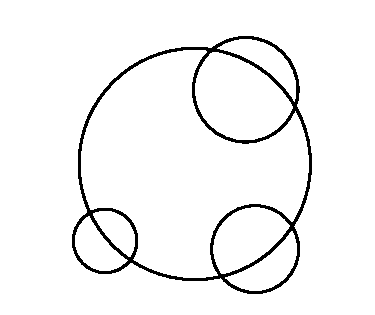
\includegraphics[scale = 0.4]{img/pivote_variante1}}\qquad\qquad
	\subfigure[El símbolo anarquista]{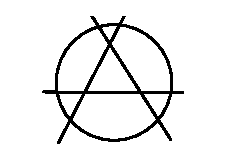
\includegraphics[scale = 0.8]{img/pivote_variante2}}
	\caption{Ilustración de conjuntos en las hipótesis de \ref{conex_cor_pivote_corte_comun}.}
\end{figure}

\begin{cor}[Cadenas]
	Sea una cadena finita $\{A_i\}_{i=1}^n$ de conexos, es decir, que verifica que $A_i\cap A_{i+1}\not=\emptyset$. Entonces $\bigcup_{i=1}^n A_i$ es conexo.
\end{cor}
\begin{proof}
	Por inducción, es claro que aplicando el teorema del pivote la cadena de dos eslabones $A_1\cup A_2$ es conexa, si suponemos que la cadena de $n$ eslabones es conexa, por el teorema del pivote, la de $n+1$ eslabones $A_{k+1}\cup\bigcup_{i=1}^k A_i$ lo será también.
\end{proof}
\begin{figure}[H]
	\centering
	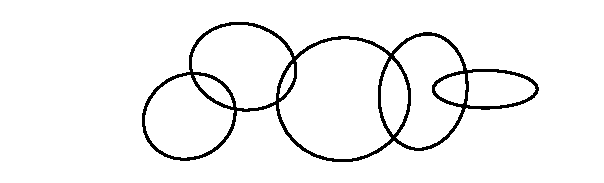
\includegraphics[scale = 0.5]{img/pivote_variante3}
	\caption{Ilustración de una cadena de conexos}
\end{figure}
\begin{obs}[Caso numerable]
	El corolario anterior también se verifica si la sucesión de conjuntos es numerable, pero no lo vamos a probar aquí.
	% AQUÍ VIENE PROBADO http://dbfin.com/topology/munkres/chapter-3/section-23-connected-spaces/problem-2-solution/
\end{obs}

El siguiente resultado, aunque también es consecuencia del teorema del pivote \ref{conex_theo_pivote}, es más que un mero corolario y merece la categoría de teorema por sí mismo.

\begin{theo}[Sandwich]\label{conex_teo_adherencia_conexa}
	Sea $A$ conexo y $B$ un conjunto emparedado entre $A$ y su adherencia, es decir, $A\subset B\subset\adher{A}$. Entonces $B$ es conexo. En particular, $\adher{A}$ es conexo.
\end{theo}
\begin{proof}
	Podemos poner nuestro conjunto $B$ de forma amigable para usar el teorema del pivote.
	\[B=\bigcup_{b\in B\setminus A} (A\cup\{b\}) \]
	como la intersección de la familia es no vacía, entonces basta probar que cada $A\cup\{b\}\subset\adher{A}$ es conexo, pues en ese caso el teorema del pivote \ref{conex_theo_pivote} nos garantiza la conexión de $B$.
	
	Si hubiera un clopen no trivial $C\subset A\cup\{b\}$, entonces, $C\cap A$ sería un clopen en $A$. Como $A$ es conexo, $C\cap A$ debe ser el vacío o el total.
	\begin{itemize}
		\item Si es el vacío, entonces $C=\{b\}$ y por tanto $\{b\}$ es abierto, luego, como el entorno $\{b\}$ de sí mismo no corta con $A$, $b\not\in\adher{A}$, lo cual es una contradicción.
		\item Si es el total, $C=A$ y por tanto $A$ es cerrado, pero $b\not\in A=\adher{A}$, que de nuevo es una contradicción. \qedhere
	\end{itemize}
\end{proof}

Recojamos los frutos de nuestra cosecha con un ejemplo, pero antes presentemos unas definiciones que harán más ágil nuestro discurrir.
\begin{defi}[Segmento]
	En $\R^n$ un segmento que une dos puntos $a$ y $b$ es el conjunto $\{ta+(1-t)b\midc t\in[0,1]\}$, que puede interpretarse como la imagen de la interpolación lineal entre $a$ y $b$, que definimos en la ecuación \eqref{interpolacion}.
\end{defi}
\begin{defi}[Convexo]
	En $\R^n$, se dice que un conjunto es \tbi{convexo} si para cada par de puntos $a,b\in E$, el segmento que los une también está en el conjunto.
\end{defi}
\begin{defi}[Estrellado]
	En $\R^n$ definimos conjunto \tbi{estrellado} como un conjunto en el que existe un punto tal que el segmento de él a cualquier otro está en el conjunto.
\end{defi}

\begin{exa}[Miscelánea]
	\label{conex_exa_miscel}
	Veamos algunos ejemplos de conjuntos conexos:
	\begin{enumerate}
		\item Los segmentos son conexos por ser la imagen continua de $[0,1]$, que es conexo, por la interpolación lineal, que es continua.
		\item Si un conjunto es convexo entonces es estrellado, y si es estrellado entonces es conexo. Además, las implicaciones recíprocas no se verifican. En resumen
		\[\text{Convexo}\ra\text{Estrellado}\ra \text{Conexo}\]
		
		En efecto, si $A$ es convexo tomando cualquier punto como ``centro de la estrella'' se deduce que $A$ es estrellado.
		
		Asimismo, si $A$ es estrellado se puede escribir como
		\[A=\bigcup_{a\in A} [a_0, a]\]
		para cierto $a_0\in A$. Cada segmento $[a_0,a]$ es conexo, y, por tanto, por el teorema del pivote, como todos comparten el punto $a_0$, su unión es conexa.
		
		Nótese que ni la convexidad ni ser estrellado son propiedades topológicas; ambas son propiedades vectoriales: su definición solo tiene sentido en un espacio que, al menos, tenga estructura de espacio vectorial.
		
		\item Una circunferencia en $\R^2$ es conexa, pero no es estrellada. En efecto, es conexa por ser la imagen de $[0,2\pi]$ por la aplicación $t\mapsto (\cos t, \sen t)$.
		
		\item El grafo de la función $\sen\frac{1}{x}$ para $x>0$, que escribimos:
		\[C = \left\{\left(x,\sen\frac{1}{x}\right)\midc x>0\right\}\]
		es conexo por ser la imagen continua de $(0,\infty)$ por la aplicación:
		\[x\mapsto \left(x,\sen\frac{1}{x}\right)\]
		
		Lo que es más interesante, para cualquier $a\in [-1,1]$ se verifica que $\{(0,a)\}$ es adherente a $C$ (es relativamente fácil de comprobar) y por tanto que $C\cup\{(0,a)\}$ es conexo.
		\begin{figure}[H]
			\centering
			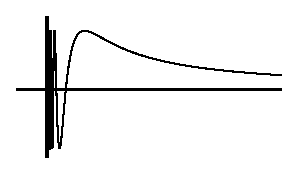
\includegraphics[scale = 0.8]{img/funcionsen1x}
			\caption{Ilustración de la gráfica de $\sen(1/x)$}
		\end{figure}
		
		\item Consideramos el conjunto:
		\begin{equation}\label{lineas}C = \big(\{0\}\times (0,1]\big) \cup \left(\bigcup_{n\in\N} [0,1]\times\left\{\frac{1}{n}\right\}\right) \end{equation}
		\begin{figure}[H]
			\centering
			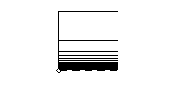
\includegraphics[scale = 0.2]{img/lineas}
			\caption{Ilustración del conjunto de la ecuación \eqref{lineas}}
		\end{figure}
		que es unión de segmentos horizontales cada vez más juntos y de un segmento vertical. Este es trivialmente conexo por el corolario \ref{conex_cor_pivote_corte_comun}. Lo particular es que si unimos a $C$ el segmento horizontal:
		\[(0,1)\times\{0\}\]
		sigue siendo conexo por ser adherencia de $C$ (¡compruébese!). 
\qedhere
	\end{enumerate}
\end{exa}

Completamos esta sección con una propiedad interesante garantizada por la conexión.

\begin{lem}[Cadena]
	Sea $\X$ conexo y $\{U_i\}_{i\in I}$ un recubrimiento por abiertos de $\X$. Dos puntos cualesquiera $x,y\in\X$ se pueden conectar mediante una cadena finita de abiertos del recubrimiento.
\end{lem}

\begin{proof}
	Sea $A=\{z\in\X \midc \text{existe una cadena de } x \text{ a } z \}$. $A$ es claramente no vacío, puesto que $x\in A$. Por ende, nuestro objetivo será ver que $\X=A$. Una forma de hacerlo será ver que $A$ es un clopen, ya que si lo fuera, por conexión de $\X$ y por ser $A$ no vacío $A$ tendría que ser el total.
	\begin{itemize}
		\item Veamos que $A$ es abierto. En efecto, dado $z\in A$, queremos ver que existe un abierto $U$ tal que $z\in U\subset A$. Si tomamos el último abierto $U$ de la cadena que une $x$ y $z$ hemos ganado, ya que $U\subset A$, ya que todo punto de $U$ queda unido con $x$ con la misma cadena que $z$.
		
		\item Ahora la clausura. En efecto, si $z\in\adher{A}$, entonces habrá un abierto $U_{i_0}$ tal que $U_{i_0}\cap A\not=\emptyset$. Considerando un punto $y$ de la intersección, como $y$ está en $A$, hay una cadena de $x$ a $y$. Uniendo $U_{i_0}$ a la cadena obtenemos una cadena de $x$ a $z$, y por tanto $z\in A$, luego $A=\adher{A}$. \qedhere
	\end{itemize}
\end{proof}
Este último resultado tiene una aplicación muy importante en los espacios euclídeos usuales.
\begin{defi}[Poligonal]
	Una \tbi{poligonal} en $\R^n$ es un conjunto $\Gamma$ de la forma\begin{equation*}
		\Gamma=[x_0,x_1]\cup[x_1,x_2]\cup\dots\cup[x_{n-2},x_{n-1}]\cup[x_{n-1},x_n]
	\end{equation*}
	Donde $[x_i,x_j]$ representa el segmento que une a los puntos $x_i$ y $x_j$. Nótese que por la variante de las cadenas del teorema del pivote una poligonal es conexa.
\end{defi}
\begin{defi}[Conexión por poligonales]
	Un conjunto $A\subset\R^n$ se dice \tbi[conexo!por poligonales]{conexo por poligonales} si dados dos puntos cualesquiera $x,y\in A$, hay una poligonal $\Gamma$ contenida en $A$ que une a $x$ y a $y$.
\end{defi}
\begin{obs}[Conexión y conexión por poligonales]
	Todo conjunto conexo por poligonales es conexo. En efecto, si tomamos un punto $a$ de $A$ y consideramos la familia de poligonales (conexos) que conectan a $a$ con el resto de puntos de $A$, tenemos que dicha familia tiene a $\{a\}$ por intersección, luego podemos aplicar el teorema del pivote, obteniendo que la unión de la familia, que es $A$, es conexa.
\end{obs}
\begin{obs}[Abiertos y conexión por poligonales]
	Podemos recubrir cualquier abierto conexo de $\R^n$ con bolas (véase el lema \ref{etop_lem_otrasProp}), y, por tanto existe una cadena de bolas que une cualquier par de puntos.
	
	Si tomamos un punto en cada intersección entre bolas consecutivas de la cadena y consideramos los segmentos que los unen, tengo una poligonal que conecta los dos puntos.
	
	De esta forma, para abiertos de $\R^n$ la conexión y la conexión por poligonales son nociones equivalentes.
\end{obs}

\section{Componentes conexas}

Al igual que ocurría con la compacidad, sería deseable que todos los espacios fuesen conexos. Dado que esto no se da, nos conformaremos con quedarnos con los subconjuntos conexos del espacio. Surge así la idea de componente conexa que definimos a continuación.

Aunque parezca que esto no es una ventaja, es tremendamente útil a la hora de estudiar, por ejemplo, si dos espacios son homeomorfos, ya que el número de componentes conexas se conserva por homeomorfismos (ver ejemplo \ref{etop_exa_homeomorfismos}).

\begin{defi}[Componente conexa de un punto]
	Se dice que un conjunto $\Co(x)\subset\X$ es una \tbi{componente conexa} de $x\in\Co(x)$ si es un conjunto conexo ``maximal''. Esto es que, dado un conjunto $D$ conexo que contiene a $x$ se verifica que $\Co(x)\not\subset D$.
	
	En general, diremos que un conjunto $\Co$ es una componente conexa si lo es de alguno de sus puntos (y por tanto de todos, véase la observación \ref{conex_obs_compartido}).
\end{defi}

Análogamente a lo que hicimos con el interior y la adherencia en el capítulo \ref{etop}, veamos que la componente conexa de un punto tiene una caracterización conjuntista muy sencilla.

\begin{lem}[Caracterización conjuntista]
	Dado $x\in\X$, el conjunto 
	$\Co(x)=\bigcup_{A\subset\X} A$ con $x\in A$ y $A$ conexo, es una componente conexa de $x$.
\end{lem}
\begin{proof}
	En efecto, $\Co(x)$ es no vacío, ya que $\{x\}$ es conexo. Además, la familia de conexos que conforma $\Co(x)$ tiene al menos a $\{x\}$ en la intersección, luego, por el teorema de pivote, $\Co(x)$ es conexo.
	
	Por construcción es, además, maximal, ya que, si hubiera un conexo que lo contuviera, este contendría a $x$, y, por tanto, estaría $\Co(x)$.
\end{proof}
\begin{obs}[Unicidad]
	\label{conex_obs_unicidad}
	Cabe destacar que $\Co(x)$ no es solo una componente conexa de $x$, sino \tb{la} componente conexa de $x$. 
	
	En efecto, si hubiera otra, digamos $E$, tanto $\Co(x)$ como $E$ deben contener a $x$, luego su intersección será no vacía $E\cap \Co(x)\not=\emptyset$. En tal caso, $A:=E\cup \Co(x)$ sería conexo por el teorema del pivote, y, como además $x\in A$, $A$ estará en la familia que conforma $\Co(x)$, luego $E\subset\Co(x)$. Como $E$ es una componente conexa se debe dar la igualdad.
\end{obs}
\begin{obs}[Intersección y contención]
	\label{conex_obs_inter}
	La observación \ref{conex_obs_unicidad}, a parte de darnos la unicidad de la componente conexa de un punto, nos viene a decir, que si un conexo corta a la componente conexa, este debe estar contenido en ella. Este hecho puede sacarnos de algún que otro apuro. 
\end{obs}
\begin{obs}[Componente conexa compartida]
	\label{conex_obs_compartido}
	Nótese que pudiera haber varios puntos con la misma componente conexa, de hecho, todos los puntos de $\Co(x)$ tienen a $\Co(x)$ por componente conexa. En efecto, sea $y\in\Co(x)$, llamemos $\Co(y)$ a su componente conexa. Es claro que, por la caracterización conjuntista $\Co(x)\subset\Co(y)$, luego, $x\in\Co(y)$, $\Co(y)$ es un conexo que contiene a $x$, por tanto, debe estar contenido en su componente conexa, es decir $\Co(y)\subset\Co(x)$.
	
	En definitiva podemos concluir que una componente conexa lo es de todos sus puntos y de ninguno más (obviamente). En particular, si un espacio es conexo, es la componente conexa de todos sus puntos.
\end{obs}

A continuación enunciamos y demostramos algunas propiedades de las componentes conexas.

\begin{lem}[Propiedades varias]
	Sea $\X$ un espacio topológico, entonces:
	\begin{enumerate}
		\item Las componentes conexas son cerradas.
		
		\item Las componentes conexas son una partición del espacio. Es decir, son disjuntas dos a dos y su unión es el total.
		
		\item Si $\X$ tiene un número finito de componentes conexas, estas son abiertas.
		\item Si en $\X$ todo punto tiene un entorno conexo, entonces las componentes conexas de $\X$ son abiertas.
	\end{enumerate}
\end{lem}
\begin{proof}
	Demostremos esto como si fuéramos a emparedar a alguien, ladrillo a ladrillo, en este caso, apartado a apartado.
	\begin{enumerate}
		\item Sea $\Co(x)$ componente conexa. Como es conexo, su adherencia es conexa ( véase el teorema del sandwich \ref{conex_teo_adherencia_conexa}), y por ser maximal $\Co(x)=\adher{\Co(x)}$.
		
		\item Es claro que
		\[\X=\bigcup_{x\in\X} \Co(x)\]
		Además, dadas dos componentes conexas, $\Co_1$ y $\Co_2$, si $\Co_1\cap\Co_2\not=\emptyset$ entonces $\Co_1\subseteq\Co_2$ y por ser maximales se daría la igualdad.
		
		\item Por hipótesis $\X=\Co_1\cup\cdots\cup\Co_r$ siendo la unión disjunta. Entonces, para cada $i\in\{1,\cdots r\}$ se tiene que 
		\[\Co_i=\X\setminus (\Co_1\cup\cdots\cup\Co_{i-1}\cup\Co_{i+1}\cup\cdots\cup\Co_r)=:\X\setminus \Co\]
		Como cada componente conexa es cerrada, y además, la unión finita de cerrados es cerrada, $\Co$ es cerrado, luego como $\Co_i=\X\backslash \Co$, es claro que $\Co_i$ es abierto para todo $i$.
		
		\item Sea $\Co$ componente conexa de $\X$, veamos que es entorno de todos sus puntos. Sea $x\in\Co$. Por hipótesis existe $\V$ entorno conexo de $x$, con lo cual $\V\cap\Co\not=\emptyset$. Esto implica que $x\in\V\subset\Co$, con lo que $\Co$ es entorno de $x$.\qedhere
	\end{enumerate}
\end{proof}
Veamos ahora una serie de ejemplos para familiarizarnos con estos conceptos.
\begin{exa}[Sucesión armónica]
	Estudiemos las componentes conexas del espacio topológico compuesto por el rango de la sucesión armónica y su límite $\X:=\{0\}\cup\{1/n\midc n\in\N\}$.
	
	Evidentemente, los puntos son conexos, el reto será pues, ver si puede haber una componente conexa $\Co$ con dos puntos distintos, digamos $x$ e $y$, sin pérdida de generalidad $x<y$.
	
	Si $\Co$ fuera conexo, por la caracterización de los conexos de la recta, debería contener a todos sus puntos intermedios, no obstante es claro que $y=1/n_0$ para cierto $n_0\in\N$, luego tomando el punto medio $c$ entre $\frac{1}{n_0+1}$ e $y$ tenemos que $c$ es un punto entre $x$ e $y$ que no está en $\X$ y por tanto no está en $\Co$. Luego los únicos conexos de $\X$ son los puntos.
	
	Además, se comprueba fácilmente que las componentes conexas de $\{1/n\midc n\in\N\}$ son abiertas, no obstante la componente conexa $\{0\}$ no es abierta (¡compruébese!).
\end{exa}
Razonando de manera similar podemos estudiar las componentes conexas de $\Q$.
\begin{exa}[Racionales] Por densidad de $\Q$ en $\R$ entre dos irracionales siempre hay un racional, luego las únicas componentes conexas de $\Q$ son los puntos. Además, ninguna de estas componentes es abierta. Esto último también se deduce de la densidad de $\Q$.
\end{exa}
Los dos ejemplos anteriores estudiaban las componentes conexas de espacios numerables, viendo que las únicas componentes conexas eran los propios puntos. Nos preguntaremos si pudiera ocurrir esto también con espacios no numerables.
\begin{exa}[Discontinuo de Cantor]
	Aunque no lo demostraremos aquí, el conjunto de Cantor $K$, que tantas propiedades nos esconde, es no numerable y sus componentes conexas son los puntos. 
\end{exa}
Veamos otro ejemplo (esta vez más sencillo) de este fenómeno.
\begin{exa}[Sorgenfrey]
	La recta de Sorgenfrey tiene por componentes conexas a los puntos, esto se debe, como veremos en el lema \ref{conex_baseClop}, a que la recta de Sorgenfrey es \kolmogorov (de hecho \hausdorff) y tiene una base de clopens (ver ejemplo \ref{etop_sorgenfrey}).  
\end{exa}
A la luz de este último ejemplo, brota cual tubérculo el siguiente lema.
\begin{lem}[Bases de clopens]
	\label{conex_baseClop}
	Si $\X$ es \kolmogorov y tiene una base $\B$ de clopens, entonces sus componentes conexas son los puntos, es decir, es \tbi{totalmente disconexo}.
\end{lem}
\begin{proof}
	Si hubiera un conexo $A$ con dos puntos distintos, digamos $a$ y $b$, al ser $\X$ \kolmogorov, habrá un entorno $B$ en $A$, sin pérdida de generalidad de $a$, que podremos tomar básico (luego clopen), tal que no contiene a $b$. Luego $b\in A\setminus B$. Como $B$ es clopen, $A\setminus B$ también lo será. Luego acabamos de particionar $A$ con dos clopens no triviales, en contra de su conexión.
\end{proof}
\section{Comportamiento de la conexión}
Llegados a este punto, para estudiar el comportamiento topológico no tenemos que hacer prácticamente nada. En efecto, veámoslo punto por punto.
\begin{itemize}
	\item Es claro que la conexión no se traslada a subespacios (no todos los subconjuntos de $\R$ son intervalos).
	\item Por su parte, como la imagen continua de conexos es conexa, los cocientes, que no son más que imágenes continuas drásticas, serán también conexos.
	\item En cuanto a la suma, ya demostramos en la observación \ref{const_obs_propiedadesSuma} que cada sumando era un clopen, luego ya en el caso de espacios suma de dos sumandos obtenemos una partición del conjunto en dos clopens. Luego la suma nunca es conexa.
\end{itemize}
Demostremos ahora con más calma que el producto de espacios conexos es conexo, para lo cual usaremos a nuestro querido teorema del pivote.
\begin{prop}[Conexión y productos]
	Si $\X$ e $\Y$ son conexos, entonces $\X\times \Y$ es conexo.
\end{prop}
\begin{proof}
	Para cualquier $x\in \X$ e $y\in \Y$ es claro que $A_y:=\X\times\{y\}$ y $B_x:=\{x\}\times \Y$ son conjuntos conexos por ser copias homeomorfas de $\X$ e $\Y$ respectivamente. Además, se tiene $A_y\cap B_x=(x,y)$, luego no vacía. Aplicando el teorema del pivote tenemos que $C_{(x,y)}=A_y\cup B_x$ es conexo. Tomando la familia de estos conjuntos, que es claro que se intersecan dos a dos y cubren el espacio, podemos aplicar el corolario \ref{conex_cor_pivote_corte_comun} para deducir que $\X\times \Y$ es conexo.
\end{proof}
Recapitulemos todo lo visto con una tabla.
\begin{table}[H]
	\centering
	\begin{tabular}{l|l|l|l|l|}
		\cline{2-5}
		& \textbf{Subespacios}    & \textbf{Cociente}       & \textbf{Producto}       & \textbf{Suma}           \\ \hline
		\multicolumn{1}{|c|}{\textbf{Conexión}} & \multicolumn{1}{c|}{No} & \multicolumn{1}{c|}{Sí*} & \multicolumn{1}{c|}{Sí} & \multicolumn{1}{c|}{No} \\ \hline
	\end{tabular}
	\caption{Tabla resumen de conexión.}
	\label{Tabla_conexion}
\end{table}
\section{Local--conexión}
\label{conex_local}
Vamos a definir la conexión local basándonos en la filosofía de la compacidad local.
\begin{defi}[Conexión local]
	Un espacio $\X$ se dice localmente conexo si cada uno de sus puntos tiene una base de entornos conexos.
\end{defi}
Presentemos un criterio general que caracteriza a los espacios localmente conexos.
\begin{prop}[Caracterización]\label{conex_prop_caracLocal}Las siguientes afirmaciones son equivalentes
	\begin{enumerate}
		\item $\X$ es localmente conexo.
		\item Las componentes conexas de todo abierto de $\X$ son abiertas.
		\item Todo punto de $\X$ tiene una base de entornos conexos y abiertos.
	\end{enumerate}
\end{prop}
\begin{proof}Realicemos el habitual círculo económico de implicaciones.
	\begin{enumerate}[align=left, leftmargin=*]
		\item[\fbox{$(1)\ra (2)$}] Sea $G$ un abierto de $\X$ y $\Co$ una componente conexa de $G$. Sea $x\in \Co$, al ser $G$ abierto, es entorno de todos sus puntos, y, por ser $\X$ localmente conexo, habrá un $\V$ entorno conexo de $x$ tal que $x\in \V\subset G$. Como $V\cap\Co\not=\emptyset$ ya que $x$ está en ambos conjuntos, y al ser $\Co$ la componente conexa de $x$ se tiene que $V\subset\Co$, con lo que se tiene el resultado.
		\item[\fbox{$(2)\ra (3)$}] Dado $x\in\X$, consideremos el conjunto de sus entornos abiertos conexos $\Va{x}$, veamos que es una base de entornos. En efecto, dado un entorno abierto de $x$, digamos $U$, $x$ estará en alguna de las componentes conexas $\Co$ de $U$, que por hipótesis son abiertas, luego $\Co\in\Va{x}$.  
		\item[\fbox{$(3)\ra (1)$}] Es evidente.\qedhere
	\end{enumerate}
\end{proof}
\section{Comportamiento de la local--conexión}
Lamentablemente, el estudio del comportamiento topológico de la conexión local no será tan sencillo como el de la conexión. Sin embargo a estas alturas ya no debería importarnos mucho, el lector ya debería estar curado de espanto.

En primer lugar cabe destacar que la imagen continua de un conjunto localmente conexo no necesariamente es localmente conexo. Sin embargo, la local--conexión se hereda a los cocientes.
\begin{prop}[Local--conexión y cocientes]
	\label{conex_prop_cocientes}
	Sea $\X$ localmente conexo y $f:\X\to\Y$ una identificación. Entonces, $\Y$ es localmente conexo.
\end{prop}
\begin{proof}
	Para comprobar esto echaremos mano de la caracterización de la local--conexión y comprobaremos que las componentes conexas de los abiertos de $\Y$ son abiertas.
	
	Sea $G$ un abierto de $\Y$ y $\Co$ una componente conexa de $G$. Como $f$ es una identificación $\Co$ será abierta si y solo si $f^{-1}(\Co)$ es abierto. Sea pues $x\in f^{-1}(\Co)$.
	
	Al ser $f$ continua $f^{-1}(G)$ es abierto. Como $\X$ es localmente conexo, habrá un entorno conexo $V$ que verifique que $x\in V\subset f^{-1}(G)$. Si aplicamos $f$ a la última desigualdad, al ser $f$ sobreyectiva se tiene que $f(V)\subset G$, siendo $f(V)$ un conexo contenido en $G$ por ser $f$ continua.
	
	Como tanto $f(V)$ como $\Co$ contienen a $f(x)$ es claro que se cortan, luego por la observación \ref{conex_obs_inter} se verifica que $f(x)\in f(V)\subset \Co$, con lo que $\Co$ es entorno de todos sus puntos.
\end{proof}
Aunque la conexión local se comporta peor que la conexión con los cocientes, se comporta un poco mejor con los subespacios, no llegándose a heredar la local--conexión a todos ellos.
\begin{lem}[Subespacios y local--conexión]
	\label{conex_lem_subesLocal}
	Si $A$ es un subespacio abierto de $\X$, siendo $\X$ localmente conexo, entonces $A$ es localmente conexo.
\end{lem}
\begin{proof}
	Como $x$ tiene una base de entornos $\Va{x}$ conexos abiertos, tomando la base relativa $\Va{x}\cap A$, veamos que es de entornos conexos.
	
	Como $U$ es abierto en $A$ si y solo si lo es en $\X$ (véase el lema \ref{etop_lem_otrasProp}), si no hay dos abiertos en $\X$ que particionen a los entornos de $\Va{x}$, tampoco los habrá que partan a los entornos $\Va{x}\cap A$, ya que es la subfamilia de los entornos de $\Va{x}$ contenidos en $A$.
\end{proof}
\begin{obs}[Contraejemplo]
	Para ver que la conexión local no se hereda en general, basta ver que $\R$ es localmente conexo ya que cada punto posee una base de intervalos, pero su subespacio $\{1/n\midc n\in\N\}\cup\{0\}$ no es localmente conexo al no tener $0$ una base de entornos conexos y abiertos. Esto es claro ya que el único conexo que es entorno de $0$ es el propio $\{0\}$, que no es abierto (¡compruébese!).
\end{obs}
Ahora le toca el turno a los productos y las sumas, que estudiaremos brevemente.
\begin{itemize}
	\item El producto de espacios localmente conexos es localmente conexo, esto se debe a que las bases de entorno del producto son productos de bases de entornos de los factores. Tomando la base de conexos correspondiente de cada factor, como el producto de conexos es conexo, se tiene el resultado.
	\item La suma de espacios localmente conexos es localmente conexa.
	
	En efecto, tomando un punto cualquiera $x$ del espacio suma, este estará en alguno de los estantes, que son homeomorfos a los sumandos vía las inclusiones. Como los sumandos son localmente conexos, $p_i^{-1}(x)$ tiene una base de entornos conexos, que se transforma por $p_i$ en una base de entornos conexos de $x$ por ser $p_i$ continua. 
\end{itemize}
Condensando todo lo visto, presentamos el resumen en forma de tabla.
\begin{table}[H]
	\centering
	\begin{tabular}{l|l|l|l|l|}
		\cline{2-5}
		& \textbf{Subespacios}                                                                      & \textbf{Cociente}       & \textbf{Producto}       & \textbf{Suma}           \\ \hline
		\multicolumn{1}{|c|}{\textbf{\begin{tabular}[c]{@{}c@{}}Local\\ conexión\end{tabular}}} & \multicolumn{1}{c|}{\begin{tabular}[c]{@{}c@{}}Sí, en el caso\\ de abiertos\end{tabular}} & \multicolumn{1}{c|}{Sí} & \multicolumn{1}{c|}{Sí} & \multicolumn{1}{c|}{Sí} \\ \hline
	\end{tabular}
	\caption{Tabla resumen de local conexión}
	\label{Tabla_localconexion}
\end{table}
Presentamos para terminar un ejemplo con objeto de aumentar la curiosidad del lector.
\begin{exa}[Conexión local y por poligonales]
	\label{conex_exa_poliLocal}
	El espacio $\X:=C\cup\{(0,0)\}$ donde $C$ es el conjunto definido en la ecuación \eqref{lineas} no es localmente conexo pero si es conexo por poligonales.
	
	La conexión por poligonales es evidente, dados dos puntos de $X$, si están en la misma recta horizontal basta con coger el segmento que los une.
	
	En caso contrario, bastaría con tomar el segmento horizontal que une al primer punto con $\{0\}\times [0,1]$, enlazándolo con el segmento vertical que llega hasta la altura del segundo punto, y, finalmente, enganchar este último al segmento horizontal que une $\{0\}\times [0,1]$ con el segundo punto. 
	
	La demostración de que no es localmente conexo es una adaptación de la demostración de que $\{1/n\midc n\in\N\}\cup\{0\}$ no es localmente conexo. Los detalles se dejan al lector.
\end{exa}
	%Para este capítulo se usará la abreviatura "cam".
\chapter{Conexión por caminos}
\label{cam}
La idea de conexión desarrollada en el capítulo anterior parece razonable, en el sentido de que un conjunto es conexo si no podemos realizar un ``corte limpio'' en dos piezas del conjunto.

No obstante, también parece razonable pensar que un conjunto será conexo si puedo ir andando de un lado a otro del mismo sin tener que dar saltos. Una aproximación a esta idea puede ser la conexión por poligonales, sin embargo, no parece lo suficientemente adecuada, ya que una circunferencia no es conexa por poligonales, pero en la mente humana está la idea de ir dando vueltas en círculos siguiendo el trazado de la circunferencia. Para formalizar esta idea nace la conexión por caminos.
\section{Generalidades sobre caminos}
Comenzamos definiendo lo que será el ingrediente estrella de este capítulo, los caminos.
\begin{defi}[Camino]
	Un \tbi{camino} en un espacio topológico $(\X,\T)$ es una aplicación continua $\sigma:[a,b]\to\X$. A los puntos $\sigma(a)$ y $\sigma(b)$ se les llama \tbi{extremos} del camino.
	
	En general, se dirá que $\sigma$ es un camino que conecta a sus extremos.
\end{defi}
Antes de meternos en harina hay que recordar estamos trabajando en espacios topológicos, es decir, aquí la intuición no vale de mucho.
\begin{obs}[Caminos densos]
	Cuando uno se imagina un camino, se imagina que la imagen del camino es una curva suave que no hace cosas demasiado extrañas, sin embargo la imagen de un camino puede ser densa en el plano. Este es el caso de la \tbi{curva de peano}, que no estudiaremos en estas notas.
\end{obs}
Al fin y al cabo los caminos no son más que parametrizaciones de subconjuntos de un espacio $\X$. Por esta razón, en ocasiones nos interesará considerar varios caminos con la misma imagen o \tbi{traza}. Veamos un procedimiento rápido, sencillo, y para toda la familia para cambiar el dominio de definición de un camino.
\begin{obs}[Reparametrización]
	\label{cam_obs_reparam}
	Si tenemos un camino $\sigma:[a,b]\to\X$ y queremos fabricarnos un camino $\tau:[c,d]\to\X$ con la misma traza que $\sigma$ basta con ceñirse al siguiente diagrama.
	\begin{equation*}
		\xymatrix{
			[a,b]\ar[r]^{\sigma}& \X\\
			[c,d]\ar[u]^{\varphi}\ar[ur]_{\tau\equiv\sigma\circ\varphi}
		}
	\end{equation*}
	Donde $\varphi$ es un homeomorfismo entre $[c,d]$ y $[a,b]$, en particular, suele usarse la interpolación lineal definida en el ejemplo \ref{etop_exa_homeomorfismos}. Nótese que $\tau$ es un camino por ser composición de funciones continuas. Además, tiene la misma imagen que $\sigma$ por ser $\varphi$ sobreyectiva.
\end{obs}
Otro problema importante es el de ``yuxtaponer'' o ``pegar'' caminos, es decir, si tenemos un camino que termina en un extremo y otro que empieza en ese mismo extremo, queremos definir un camino cuya traza sea la unión de las trazas de ambos caminos. A continuación presentamos un procedimiento para resolver este problema.
\begin{obs}[Pegado de caminos]
	\label{cam_obs_pegado}
	Supongamos que tenemos dos caminos $\sigma:[a,b]\to\X$ y $\tau:[c,d]\to\X$ tales que $\sigma(b)=\tau(c)$. Queremos ``soldar'' estos caminos como si fuéramos un herremos vikingo. Para ello, haremos uso de nuestro martillo, la observación \ref{cam_obs_reparam}.
	
	Observemos que bastaría con tomar, por ejemplo, las reparametrizaciones $\widehat{\sigma}:[0,\frac{1}{2}]\to\X$ y $\widehat{\tau}:[\frac{1}{2},1]\to\X$ y definir la aplicación
	\begin{equation*}
		\sigma\tau:=\left\{\begin{array}{cc}
			t\mapsto \widehat{\sigma}(t)&\text{ si }t\in[0,\frac{1}{2}]\\
			t\mapsto \widehat{\tau}(t)&\text{ si }t\in[\frac{1}{2},1]
		\end{array}\right.
	\end{equation*}
	Nótese que $\sigma\tau$ es un camino. Para comprobarlo basta ver que tenemos un recubrimiento cerrado conformado por $[0,\frac{1}{2}]$ y $[\frac{1}{2},1]$ tal que la restricción $\sigma\tau$ a cada uno de los cerrados del recubrimiento es continua (al coincidir con $\sigma$ y con $\tau$).
\end{obs}
\section{Conexión por caminos}
Comenzamos definiendo la noción de conexión por caminos.
\begin{defi}[Conexo por caminos]
	Un espacio $\X$ se dice \tbi[conexo!por caminos]{conexo por caminos} si para cualesquiera dos puntos de $\X$ hay un camino en $\X$ que los conecta.
\end{defi}
Una de las incógnitas que nos surgen al plantearnos una nueva noción de cualquier cosa es si esta es más fuerte o más débil que la que teníamos antes. En este caso, la conexión por caminos es más fuerte que la conexión ``a palo seco''.
\begin{prop}[Caminos y conexión]
	Si $\X$ es conexo por caminos, entonces $\X$ es conexo.
\end{prop}
\begin{proof}
	Evidentemente, si $\X$ es conexo por caminos podemos fijar un $x_0\in X$ y escribir $\X$ como $\X=\bigcup_{x\in\X}\Tr(\sigma_x)$, donde $\Tr(\sigma_x)$ denota a la traza del camino que conecta $x_0$ con $x$. Como los caminos son conexos por ser la imagen continua de un intervalo, la familia de conjuntos que conforma la unión es una familia de conexos, además, una familia de conexos cuya intersección contiene al menos a $x_0$. Luego, por el teorema del pivote $\X$ es conexo.
\end{proof}
Hay numerosos contraejemplos para ver que el recíproco no se cumple, veamos uno de ellos con todo lujo de detalles técnicos.
\begin{exa}[Seno del topólogo]
	\label{cam_exa_seno}
	Consideremos el conjunto conexo (ver ejemplo \ref{conex_exa_miscel}) \[\adher{\Gamma}:=\left\{\left(x,\sen\left(\frac{1}{x}\right)\right)\midc x>0\right\}\cup\{0\}\times[-1,1]=:\Gamma\cup P\]
	Evidentemente, el miembro de la izquierda de la unión es conexo, por caminos, por tanto los problemas podrán presentarse únicamente al tratar de unir un punto de $P$ con otro $\Gamma$.
	
	Sean pues $a\in P$ y $b\in \Gamma$. Supongamos que hay un camino $\sigma\equiv(\sigma_1,\sigma_2):[0,1]\to\adher{\Gamma}$ que conecta $a$ y $b$. A continuación desarrollamos un argumento basado en sucesiones para ver que esto no es posible.
	
	Tomemos $t_0:=\sup\{t\in[0,1]\midc \sigma_1(t)=0\}$, es decir, intuitivamente, el último momento en el que el camino pasa por $P$. Este supremo está bien definido por ser $A:=\{t\in[0,1]\midc \sigma_1(t)=0\}$ un conjunto acotado. Además es cerrado, ya que $A=\sigma_1^{-1}(\{0\})$, luego $A$ contiene a todos sus puntos de acumulación, en particular a su supremo, por tanto $t_0=\max A$. Esto quiere decir, que para todo $t>t_0$ se cumplirá que $\sigma_1(t)>0$.
	
	Escogemos ahora un $(0,c)\in P$ de manera que $c\not=\sigma_2(t_0)$. Hecho esto, consideramos las intersecciones de la recta horizontal $y=c$ con $\Gamma$. la primera coordenada de estas intersecciones conforman el conjunto $S:=\{(k\arcsen(c))^{-1}\midc k\in\N\}$, que puede ser entendido como una sucesión $\{x_k\}_{k=1}^\infty$.
	
	Como $\{x_k\}_{k=1}^\infty$ converge a $0$ habrá un $k_0$ a partir del cual todos los términos de la sucesión estén ``a la izquierda'' de $b$.
	
	Consideramos pues la sucesión $\{t_k\}_{k=k_0}^\infty\subset[t_0,1]$ tal que $\sigma_1(t_k)=x_k$. Al ser esta sucesión un conjunto infinito en un compacto (y al encontrarnos en $\R$) por el teorema de Bolzano--Weierstrass deberá tener una subsucesión convergente, digamos $\{t_{k_l}\}_{l=1}^\infty$ tal que $\lim t_{k_l}=:t_1$.
	
	Por continuidad de $\sigma_1$, se tiene la subsucesión $\{\sigma_1(t_{k_l})\}_{l=1}^\infty=\{x_{k_l}\}_{l=1}^\infty$ convergerá a $\sigma_1(t_1)$. No obstante, como toda subsucesión de una sucesión convergente debe converger al límite de la sucesión original se tiene que $\sigma(t_1)=0$, luego, como $t_1\in[t_0,1]$ a la fuerza se tiene que dar la igualdad $t_1 = t_0$ (por la definición de $t_0$).
	
	Ahora, repitiendo el proceso anterior con $\sigma$ en lugar de con $\sigma_1$ obtenemos que, por continuidad de $\sigma$, la subsucesión $\{\sigma(t_{k_l})\}_{l=1}^\infty=\{(x_{k_l},c)\}_{l=1}^\infty$ convergerá tanto a $\sigma(t_0)=(0,\sigma_2(t_0))$ como a $(0,c)$. Sin embargo, como el límite es único en espacios métricos y $c\not=\sigma_2(t_0)$, acabamos de llegar a un absurdo, concluyendo al fin que el seno del topólogo no es conexo por caminos.
\end{exa}
Una de esas cosas que nos hace volver a creer en la especie humana son los teoremas bonitos. Y el siguiente, que es un análogo del teorema del pivote para la conexión por caminos, lo es sin duda alguna.
\begin{theo}[Teorema del pivote]
	Sea $\{A_i\}_{i\in I}$ una familia de conexos por caminos con intersección no vacía. Entonces se verifica que la unión de la familia es conexa por caminos.
\end{theo}
\begin{proof}
	Sea $p$ un punto de la unión de la familia, luego habrá un índice $i_0$ para el cual $p\in A_{i_0}$, Además, como la intersección de la familia es no vacía, habrá un punto $a$ que esté en todos los miembros de la familia, en particular en $A_{i_0}$.
	
	Como $A_{i_0}$ es conexo por caminos habrá un camino $\sigma$ que conecte $p$ y $a$. Tomando otro punto $q$ en la unión de la familia, habrá un índice $i_1$ tal que $q\in A_{i_1}$. Como $a\in A_{i_1}$ y $A_{i_1}$ es conexo por caminos, habrá un camino $\tau$ que conecte $a$ con $q$.
	
	Pegando $\sigma$ y $\tau$ conseguimos un camino que une $p$ y $q$, y, como la elección de estos dos es arbitraria, hemos terminado.
\end{proof}
Todos los corolarios y variantes del teorema del pivote válidas para la conexión ``normal'' siguen teniendo poder aquí, y las demostraciones son exactamente las mismas, por tanto, consideramos este un buen momento para ir atrás en el tiempo y recordarlas. 
\section{Componentes conexas por caminos}
En esta sección estudiaremos el concepto análogo al de las componentes conexas, pero para esta noción de conexión. La mayoría de las propiedades de las componentes conexas se heredan (gracias al análogo al teorema del pivote) para componentes conexas por caminos con exactamente la misma prueba. De este modo, aquí nos limitaremos a enunciarlas, recalcando únicamente las diferencias con respecto a la conexión.
\begin{defi}[Componente conexa por caminos]
	Dado un punto $x$ de un espacio $\X$ se dice que un conjunto $\Co(x)$ que contiene a $x$ es una \tbi[componente conexa!por caminos]{componente conexa por caminos} de $x$ si $\Co(x)$ es un conjunto conexo ``maximal''. Es decir, dado un conjunto $D$ conexo por caminos que contenga a $x$, se verifica que $\Co(x)\not\subset D$.
	
	En general, se dirá que $\Co$ es una componente conexa por caminos si lo es de alguno de sus puntos (luego de todos, como veremos más adelante).
\end{defi}
A continuación enunciamos las propiedades más básicas de las componentes conexas por caminos, propiedades compartidas con las componentes conexas.
\begin{obs}[Propiedades compartidas]Del teorema del pivote se sigue
	\begin{enumerate}
		\item Una componente conexa por caminos de $x$ puede escribirse como $\Co(x)=\bigcup_{A\subset\X}A$ con $x\in A$ y $A$ conexo por caminos.
		\item Se cumple que la componente por caminos conexa de un punto no es solo un conjunto conexo por caminos maximal, sino máximo. Esto se traduce en que un punto posee una única componente conexa por caminos $\Co(x)$.
		\item Si un conjunto $D$ conexo por caminos corta a la componente conexa por caminos $\Co(x)$ de $x$ se verifica que $D\subset \Co(x)$.
		\item $\Co(x)$ es la componente conexa por caminos de todos sus puntos (y de ninguno más). En particular, si un espacio es conexo por caminos, este consta de una única componente conexa por caminos.
		\item Las componentes conexas por caminos conforman una partición del espacio.
		\item Si todo punto tiene un entorno conexo por caminos, entonces las componentes conexas por caminos son abiertas.\qedhere
	\end{enumerate}
\end{obs}
Vistas las similitudes con la noción usual de conexión pasemos a las diferencias, que no son pocas, aunque si sutiles.
\begin{obs}[Propiedades disonantes]
	Como no todo es este mundo es alegría y color, pues entonces viviríamos en un panal y nos llamaríamos Maya, presentamos algunas propiedades que nos obstaculizarán el discurrir.
	\begin{enumerate}
		\item Sea $\Co(x)$ la componente conexa por caminos de $x$, como $\Co$ es conexa por caminos, es conexa, luego $\Co\subset E$, siendo $E$ la componente conexa de $x$. Este último contenido podría ser estricto, como ocurre con el seno del topólogo (ver ejemplo \ref{cam_exa_seno}), que consta de dos componentes conexas por caminos y una única componente conexa.
		\item Las componentes conexas por caminos no son necesariamente cerradas, un ejemplo de esto es también el seno del topólogo, pues $\Gamma$ es una componente conexa por caminos y $\Gamma\not=\adher{\Gamma}$\qedhere
	\end{enumerate}
\end{obs}
\section{Local--conexión por caminos}
En esta sección trataremos de definir la versión local de la conexión por caminos de una forma totalmente simétrica a como lo hicimos en la sección \ref{conex_local}.
\begin{defi}[Localmente conexo por caminos]
	Un espacio $\X$ se dice \tbi{localmente conexo por caminos} si todo punto del espacio tiene una base de entornos conexos por caminos.
\end{defi}
Sin más dilación vamos a caracterizar, como hicimos en el capítulo anterior, la versión local de esta noción de conexión.
\begin{lem}[Caracterización]
	\label{cam_lem_caracter}
	Las siguientes afirmaciones son equivalentes.
	\begin{enumerate}
		\item $\X$ es localmente conexo por caminos.
		\item Las componentes conexas por caminos de de los abiertos de $\X$ son abiertas.
		\item Cada punto de $\X$ tiene una base de entornos conexos por caminos y abiertos.
	\end{enumerate}
\end{lem}
\begin{proof}
	La prueba es exactamente la misma a la de la proposición \ref{conex_prop_caracLocal}, esto se debe a que las propiedades de las componentes conexas usadas en aquella prueba son heredadas por las componentes conexas por caminos.
\end{proof}
Esta vez, la local--conexión por caminos nos aporta algo más, una condición suficiente para que un conjunto sea conexo por caminos.
\begin{prop}[Condición suficiente]
	\label{cam_prop_condSuf}
	Si $\X$ es conexo y localmente conexo por caminos, entonces $\X$ es conexo por caminos.
\end{prop}
\begin{proof}
	Consideremos la componente conexa por caminos de un punto $x$, digamos $\Co(x)$, y tratemos de ver que es el total.
	
	Por ser $\X$ localmente conexo por caminos $\Co(x)$ es un abierto no vacío. No obstante, resulta que $\X\setminus \Co(x)$ también es un abierto. Si fuera no vacío habríamos partido $\X$ con dos abiertos no triviales, entrando en contradicción con su conexión. 
\end{proof}
\section{Comportamiento topológico}
Presentamos esta vez, para variar, la tabla--resumen al comienzo la sección. A continuación iremos estudiando caso por caso el comportamiento topológico de las diferentes nociones de conexión introducidas en este capítulo.
\begin{table}[H]
	\centering
	\begin{tabular}{c|c|c|c|c|}
		\cline{2-5}
		\multicolumn{1}{l|}{}                                                                                  & \multicolumn{1}{l|}{\textbf{Subespacios}}                             & \multicolumn{1}{l|}{\textbf{Cociente}} & \multicolumn{1}{l|}{\textbf{Producto}} & \multicolumn{1}{l|}{\textbf{Suma}} \\ \hline
		\multicolumn{1}{|c|}{\textbf{\begin{tabular}[c]{@{}c@{}}Conexo por\\ caminos\end{tabular}}}            & No                                                                    & Sí*                                     & Sí                                     & No                                 \\ \hline
		\multicolumn{1}{|c|}{\textbf{\begin{tabular}[c]{@{}c@{}}Localmente conexo\\ por caminos\end{tabular}}} & \begin{tabular}[c]{@{}c@{}}Sí, en el caso \\ de abiertos\end{tabular} & Sí                                     & Sí                                     & Sí                                 \\ \hline
	\end{tabular}
	\caption{Tabla resumen de conexión por caminos}
	\label{Tabla_conexion_caminos}
\end{table}
En primer lugar pongamos en marca la cosechadora rápida y deduzcamos todo lo que podamos apoyándonos en resultados anteriores.
\begin{itemize}
	\item Es claro que la conexión por caminos no se traslada a subespacios, basta observar el plano $\R^2$ y el seno del topólogo.
	\item La suma de espacios topológicos nunca es conexa, mucho menos conexa por caminos.
	\item La suma de espacios localmente conexos por caminos es localmente conexa por caminos. Esto se deja como ejercicio, ya que la demostración es, literalmente, copiar la demostración para el caso de la local--conexión.
	\item La local--conexión por caminos se traslada a subespacios abiertos. La demostración de este hecho es exactamente la misma que la del lema \ref{conex_lem_subesLocal}.
	\item La conexión local por caminos se hereda a cocientes, no obstante, la imagen continua de un localmente conexo por caminos no tendría por qué ser localmente conexa por caminos. La demostración de este hecho es la misma que la de la proposición \ref{conex_prop_cocientes}.
\end{itemize}
Tras haber recogido los frutos de nuestro trabajo nos toca trabajar de nuevo para deducir las propiedades que nos quedan. Prometemos que no será muy doloroso.
\begin{prop}[Continuidad y conexión por caminos]
	La imagen continua de un espacio conexo por caminos es conexo por caminos.
\end{prop}
\begin{proof}
	Si $\X$ es conexo por caminos y $f$ es una aplicación continua, dados dos puntos $y$ e $y'$ que viven en $f(\X)$, habrá otros dos puntos $x$ y $x'$ de $\X$ tales que $f(x)=y$ y $f(x')=y'$. Como hay un camino $\sigma$ que conecta $x$ y $x'$, basta con considerar el camino $f\circ \sigma$ que conecta $y$ con $y'$.
\end{proof}
\begin{obs}[Conexión por caminos y cocientes]
	Del hecho de que la imagen continua de conexos por caminos sea conexa por caminos se deduce, como ya hemos hecho en otras ocasiones, que el cociente de un espacio conexo por caminos es conexo por caminos.
\end{obs}
Pasemos a estudiar los productos.
\begin{prop}[Conexión por caminos y productos]
	El producto de espacios conexos por caminos es conexo por caminos.
\end{prop}
\begin{proof}
	Sean los puntos $(x_0,y_0)$ y $(x_1,y_1)$ del espacio producto $\X\times \Y$. Es claro que habrá un camino $\sigma$ que conecte $x_0$ con $x_1$ en $\X$, y, análogamente, habrá un camino $\tau$ en $\Y$ que conecte $y_0$ con $y_1$. Sin pérdida de generalidad podemos suponer que ambos caminos tienen a $[0,1]$ por domino. 
	
	Considerando el camino $\gamma\equiv(\sigma,\tau)$ tenemos que $\gamma$ conecta a $(x_0,y_0)$ con $(x_1,y_1)$.
\end{proof}
\begin{cor}[Local--conexión por caminos y productos]
	El producto de espacios localmente conexos por caminos es localmente conexo por caminos.
\end{cor}
\begin{proof}
	Sea $(x,y)$ un punto del espacio producto, es claro que $x$ tiene una base de entornos conexos por caminos $\Va{x}$ en $\X$ mientras que $y$ tiene otra base de entornos conexos por caminos $\Va{y}$ en $\Y$. Como el producto de bases de entornos es base de entornos del producto, basta con tomar la base de entornos $\Va{x}\times\Va{y}$, cuyos entornos son conexos por caminos por la proposición anterior.
\end{proof}
Veamos aquí de forma condensada las pintorescas relaciones entre las distintas formas de ver la conexión.
\begin{figure}[h!]
	\centering
	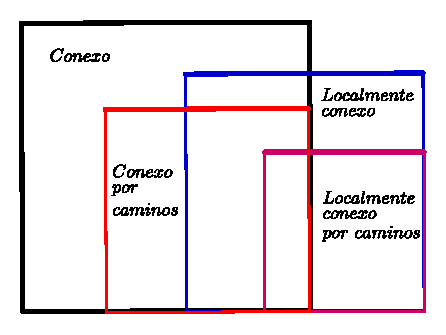
\includegraphics[scale = 1]{img/Comparacion_conexion}
	\caption{Ilustración de las relaciones entre las diferentes nociones de conexión.}
\end{figure}
Veamos un ejemplo de cada, asegurándonos de que hemos hecho bien el dibujo.
\begin{exa}[Ejemplos y contraejemplos]\
	\begin{enumerate}
		\item En la proposición \ref{cam_prop_condSuf} demostramos que un conjunto conexo y localmente conexo por caminos debe ser conexo por caminos, con lo que el dibujo es un fiel reflejo de la realidad, al menos en ese punto.
		\item A la hora de encontrar un espacio conexo por caminos y no localmente conexo nos bastará con coger el conjunto del ejemplo \ref{conex_exa_poliLocal}.
		\item Si al conjunto del ejemplo  \ref{conex_exa_poliLocal} le quitamos el punto $(0,0)$ obtenemos un conjunto conexo, no conexo por caminos que no es localmente conexo.\qedhere
	\end{enumerate}
\end{exa}
Encontrar los contraejemplos restantes requiere un poco más de valor, sangre, sudor, y, por supuesto, muchas lágrimas.
\begin{exa}[Conexo, localmente conexo y no conexo por caminos]
	La recta real con la topología de los complementarios numerables $(\R,\T_{\text{CN}})$ es claramente conexa, ya que dos abiertos cualesquiera se cortan, en efecto, si dos abiertos no triviales $U\cap V=\emptyset$ entonces, tomando complementarios tendríamos que $\R$ es numerable, lo cual es absurdo.
	
	Además, todo abierto $U$ es conexo, esto se debe a que los abiertos relativos de un abierto son los abiertos del espacio ambiente contenidos en $U$. De aquí se deduce que $(\R,\T_{\text{CN}})$ es localmente conexo, ya que basta tomar como base de entornos conexos de un punto $x$ a todos los abiertos que contienen a $x$.
	
	Para ver que no es conexo por caminos usaremos una forma de discurrir muy útil. Supongamos que hay una aplicación $\sigma:[0,1]\to\R$ que conecta dos puntos, digamos $x$ e $y$, y veamos qué debe cumplir para ser un camino.
	
	Si $\sigma$ fuera un camino, entonces $K:=\sigma([0,1])$ sería compacto y conexo. Si $K$ fuera infinito, tendría un subconjunto $F$ numerable, y por tanto cerrado, luego compacto, por ser un cerrado en un compacto. Sin embargo, la topología relativa de $F$ es la discreta por ser un conjunto numerable, lo cual entra en contradicción con su compacidad.
	
	Esto solo nos deja la salida de que $K$ sea finito, y por tanto, $K$ tiene inducida la topología discreta. Como $K$ debe ser también conexo, $K$ tendrá que ser unipuntual. Esto quiere decir que los caminos de $(\R,\T_{\text{CN}})$ únicamente pueden contener a un punto en su traza. Dicho de otra manera, $(\R,\T_{\text{CN}})$ es totalmente disconexo por caminos.
\end{exa}
Únicamente nos queda por encontrar un espacio conexo por caminos, localmente conexo, pero no localmente conexo por caminos. Para ello, de nuevo debemos dibujar un pentagrama en el suelo y rezar $n$ salmos en arameo antiguo.
\begin{exa}[Productos y cocientes de Satán]
	Veamos que el espacio $\X$, definido como sigue, cumple lo que queremos. \[\X:=\frac{[0,1]\times \R}{\{1\}\times \R}\] donde $[0,1]$ tiene la topología usual y $\R$ viene equipado con la topología de los complementarios numerables. La relación de equivalencia que induce este cociente no es más que la que hace corresponder a cada punto consigo mismo e identifica a todos los puntos del segmento $\{1\}\times\R$.
	
	Como los dos factores del producto son localmente conexos, el producto también lo será, así como su cociente. Luego $\X$ es localmente conexo.
	
	$\X$ es conexo por caminos, esto lo deducimos del teorema del pivote. Es claro que cada segmento $y=a$ con $a\in\R$ es un subespacio de $\X$ homeomorfo a $[0,1]$, luego un camino (¡compruébese!). Por tanto, los segmentos $y=a$ son conexos por caminos.
	
	Como la familia de todos estos segmentos cortan a $\{1\}\times \R$, que es un punto de $\X$, hemos encontrado una familia de conexos por caminos de intersección no vacía, que además, cubre el espacio. Esto, por el teorema del pivote quiere decir que $\X$ es conexos por caminos.
	
	Ahora veamos que $\X$ no es localmente conexo por caminos, para ello, tenemos una maravillosa caracterización que nos dice que si lo fuera, entonces los abiertos serían localmente conexos por caminos (ver el lema \ref{cam_lem_caracter} y reflexionar sobre él).
	
	Nuestra tarea pues es encontrar un abierto que no sea localmente conexo por caminos, con un poco de magia encontramos que $A:=\X\setminus (\{1\}\times \R)=[0,1)\times\R$ es un abierto de $\X$ por ser la proyección de un abierto saturado.
	
	$A$ no es localmente conexo por caminos, ya que, al considerar la proyección $p_1$, que es una identificación (por ser sobreyectiva y abierta), luego transforma conserva la local--conexión por caminos, tendríamos que $p_1(A)=\R$. De aquí se desprende que $\R$ con la topología de los complementarios numerables sería localmente conexo por caminos, lo cual es falso.
	
	En efecto, las únicas componentes conexas por caminos de $\R$ son los puntos, que son cerrados, entrando en contradicción con el lema \ref{cam_lem_caracter}.
\end{exa}
Dicho esto, nuestro viaje por la topología general ha concluido. Pero aun debemos cruzar una última frontera, adentrándonos en las entrañas del abstruso, pero a la vez maravilloso mundo de la topología algebraica.
	
	\part{Topología algebraica}
	%Para este capítulo se usará la abreviatura "grf".
\chapter{Grupo fundamental}
\label{grf}

La topología algebraica comprende métodos que son significativamente distintos a los empleados hasta ahora en topología general. Intenta asignar a un espacio topológico algún invariante algebraico (por ejemplo, un grupo) y utilizar las propiedades de este invariante para obtener información sobre la topología. Este capítulo se centrará, pues, en el estudio del grupo fundamental, que es uno de estos invariantes.

\section{Homotopía}

En particular, introducimos la homotopía con el propósito de definir más adelante la noción de grupo fundamental. La idea que tratamos de modelizar con la homotopía es la de deformar continuamente un camino en otro. Sin embargo, definiremos algo bastante más general. 

\begin{defi}[Homotopía]
	Dados dos espacios topológicos, una \tbi{homotopía} es simplemente una aplicación continua $H:\Y\times [0,1]\to \X$. Normalmente escribiremos $H_s(y) \coloneqq H(y,s)$. 
\end{defi}
Un pequeño dibujo y una observación nos ayudarán a afianzar este nuevo concepto.
\begin{figure}[h!]
	\centering
	\label{grf_homotopia1}
	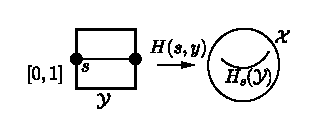
\includegraphics[scale = 1]{img/homotopia1}
	\caption{Representación geométrica de una homotopía.}
\end{figure}
\begin{obs}[Familia continua]
	Como una aplicación (en particular una homotopía) $H$ es continua si y solo si dado un recubrimiento cerrado (por ejemplo $\{s\}\times\Y$ con $s\in[0,1]$), su restricción continúa siendo continua en cada cerrado del recubrimiento, tenemos que una homotopía puede ser entendida como una ``familia continua'' de aplicaciones continuas $\Y\to\X$. Esto se debe a que, $\{s\}\times\Y$ es homeomorfo a $\Y$. Escrito de forma conjuntista.
	\begin{equation*}
		H\equiv\{H_s:\{s\}\times\Y\to\X\midc s\in[0,1]\}
	\end{equation*}
	Generalmente daremos nombres concretos a las aplicaciones $H_0$ y $H_1$, por ejemplo $f$ y $g$.
\end{obs}
Definimos a continuación la relación de homotopía entre funciones.
\begin{defi}[Funciones homótopas]
	Sean $f,g:\Y\to\X$ aplicaciones. Diremos que $f$ y $g$ son \tbi[aplicación!homótopa a otra]{homótopas} si existe, una homotopía $H$ que verifica $H_0(y)=f(y)$, $H_1(y)=g(y)$. En tal caso se dirá que $H$ es una homotopía entre $f$ y $g$.
	
	Si $f$ y $g$ son homótopas escribiremos $f\homot g$.
\end{defi}
Hechas todas estas disquisiciones iniciales, paremos al caso que pretendíamos modelizar desde el principio (y el que se ajusta al dibujo de la figura \ref{grf_homotopia1})
\begin{obs}[Caminos homótopos]
	\indexg{homotopía!de caminos}
	Un caso particular importantísimo de homotopía es la homotopía de caminos. Como se sigue directamente de la definición de homotopía, dos caminos $\sigma,\tau:[0,1]\to\X$ son homótopos si existe una homotopía $H:[0,1]\times [0,1]\to\X$, de forma que $H_0\equiv\sigma$ y $H_1\equiv\tau$.
\end{obs} 
Un propiedad crucial de las homotopías es que inducen una relación de equivalencia, como demostramos a continuación.
\begin{prop}[Equivalencia]
	La relación de homotopía ${\homot}$ es una relación de equivalencia.
\end{prop}
\begin{proof}
	Basta ver que es reflexiva, simétrica y transitiva:
	\begin{enumerate}
		\item Es reflexiva, pues, dada una función $f$, la homotopía definida por $H_s(y) = f(y)$ para todo $s\in[0,1]$ es, en efecto, homotopía entre $f$ y $f$.
		\item Es simétrica, ya que dadas funciones $f\homot g$ relacionadas por una homotopía $H$, consideramos la aplicación $H'_s(y):=H(y,1-s)$, que es una homotopía $g\homot f$ por ser composición de funciones continuas. Intuitivamente, estamos recorriendo el cuadrado de la figura \ref{grf_homotopia1} de arriba hacia abajo.
		\item Es transitiva, ya que, dadas funciones $f\homot g$, $g\homot h$, con sendas homotopías asociadas $H^1, H^2$, definimos
		\[H_s(y) := \left\{\begin{array}{ll}
		H^1_{2s}(y) & \text{ si } s\in [0,\frac{1}{2}] \\
		H^2_{2s - 1}(y) & \text{ si } s\in [\frac{1}{2},1] 
		\end{array}\right.\]
		que está bien definida y es homotopía, además, se verifica que $f\homot h$ vía $H$. \qedhere  
	\end{enumerate}
\end{proof}
Antes de continuar introduzcamos una pequeña definición.
\begin{defi}[Nulhomótopa]
	Decimos que una aplicación $f:\Y\to\X$ es \tbi[aplicación!nulhomótopa]{nulhomótopa} si $f$ es homótopa a alguna aplicación constante.
\end{defi}
Veamos un primer resultado referente a la nulhomotopía que nos puede dejar un poco consternados a primera vista, pero que con una visión geométrica resulta bastante natural.
\begin{exa}[Nulhomotopías en convexos]
	\label{grf_nulhomotopias_convexos}
	Consideramos $\X\subset\R^n$ convexo. En este caso, cualquier aplicación $f:\Y\to\X$ continua es nulhomótopa.
	
	En efecto, sea $a\in X$ (nuestra aplicación constante). Consideramos la homotopía
	\[H_s\equiv(1-s)f+sa\]
	que está definida en $\X$, pues, al ser este convexo, $[f(y),a]\subset\X$ para cualquier $y\in \Y$. Entonces, se verifica
	\[\begin{array}{l}
	H_0(y)=f(y) \\
	H_1(y)=a
	\end{array}\]
	que es precisamente lo que buscábamos. Nótese que si $\X$ es estrellado en lugar de convexo, se verifica la misma propiedad y la demostración es totalmente análoga, tomando $a$ el ``centro'' del estrellado.
	
	La homotopía definida de esta forma se llama \tbi{interpolación lineal}, y es asombrosamente útil teniendo en cuenta su sencillez. Merece la pena notar que, cuando está bien definida, es siempre homotopía (por ser composición de funciones continuas). Sin embargo, habrá muchos contextos en los que no esté bien definida.
\end{exa}
Introducimos una nueva definición que nos será útil en el futuro inmediato.
\begin{defi}[Contráctil]
	Decimos que un espacio topológico $\X$ es \tbi[espacio!contráctil]{contráctil} si $\Id_\X$ es nulhomótopa.
\end{defi}

\begin{obs}[Convexos y estrellados]
	Como, por el ejemplo \ref{grf_nulhomotopias_convexos}, sabemos que todas las aplicaciones que llegan a un espacio convexo o estrellado son nulhomótopas, entonces está claro que cualquier convexo o estrellado es contráctil.
\end{obs}

La siguiente proposición sirve al mismo tiempo como ejemplo y como enunciado de un resultado que nos será útil un poco más adelante, cuando estudiemos las esferas.

En particular, buscamos condiciones suficientes para que dos aplicaciones sean homótopas en la esfera.
\begin{prop}[La esfera $\esfera^n$]
	\label{grf_prop_esfera_no_sobre_nulhomotopa}
	Si $f,g:\Y\to\Sfe^n$ continuas tales que verifican que $f(y)\neq -g(y)$ para todo $y\in\Y$. Es decir, $f$ y $g$ no tienen puntos antipodales, entonces $f\homot g$.
	
	En particular, si $f:\Y\to\Sfe^n$ no es sobreyectiva, entonces es nulhomótopa.
\end{prop}
\begin{proof}
	Nuestro corazón nos dice que la interpolación lineal es una buena idea, pero nuestra fría cabeza nos dice que en las esferas no está bien definida. Sin embargo, si ``unitarizamos'' la interpolación lineal podemos sacar algo de petróleo. Definimos la homotopía $H$ como
	\[H_s(y)=\frac{(1-s)f(y)+sg(y)}{\norm{(1-s)f(y)+sg(y)}}\]
	Desde luego, está siempre en $\Sfe^n$ como debe ocurrir. Entonces, solo falta para ver que está bien definida, probar que existe en todo punto, y para ello necesitaremos la hipótesis.
	
	En efecto, las imágenes de $f$ y $g$ son puntos de la esfera unidad, y por tanto son vectores de norma $1$. Si $f(y)$ y $g(y)$ no son puntos antipodales, entonces hay dos opciones:
	\begin{itemize}
		\item $f(y)=g(y)$, pero como $s>0$, $1-s>0$ es imposible que $(1-s)f(y)+sg(y) = 0$.
		\item $f(y)$ y $g(y)$ son linealmente independientes, luego ninguna combinación lineal suya con coeficientes no nulos puede sumar $0$.
	\end{itemize}
	
	Y ya hemos terminado, porque está bien definida y desde luego es continua (al ser $f$, $g$ continuas, y la norma una función continua, es continua por ser suma, producto y cociente de aplicaciones continuas en $\R^n$). Entonces es homotopía.
	
	Para el caso particular, consideramos $a$ tal que $-a\not\in f(\Y)$, lo cual podemos conseguir por no ser sobreyectiva. Solo queda definir la homotopía anterior con $g\equiv a$.
\end{proof}
La siguiente observación da una vuelta de tuerca a esto último.
\begin{obs}[Visión alternativa]
	El hecho de que si $f:\Y\to\Sfe^n$ no es sobreyectiva entonces es nulhomótopa se puede plantear desde el punto de vista de la naturaleza topológica de la esfera. En efecto, $f(\Y)\subset\Sfe^n\setminus\{b\}$ para algún punto $b$, y resulta que, con una modificación de la proyección estereográfica se puede demostrar que esto es homeomorfo a $\R^n$, que es convexo y por tanto $f$ es nulhomótopa. Lo mejor para entender esto es hacerse un dibujillo.
\end{obs}

A veces, nos interesará que la homotopía entre dos funciones mantenga invariante alguna propiedad extra. En particular, solemos necesitar que algunos puntos no se muevan de su posición al homotopar.
\begin{defi}[Homotopía relativa]
	Una homotopía $H:\Y\times[0,1]\to\X$ se llama \tbi[homotopía!relativa]{relativa} a un subconjunto $A\subset\Y$ cuando $H_s(a)=H_0(a)$ para todo $a\in A$ y para todo $s\in [0,1]$. En particular, $H_0\equiv H_1$ en $A$. Se suele escribir $H_s:f\homot[A]g$.
\end{defi}

La definición que sigue, caso particular de la anterior, es absolutamente imprescindible para el estudio del grupo fundamental que vamos a realizar a lo largo de este capítulo.

\begin{defi}[Homotopía de extremos fijos]
	Decimos que dos caminos $\sigma,\tau:[0,1]\to\X$ son \tbi[homótopía!de extremos fijos]{homótopos con extremos fijos} si son homótopos relativos a $\{0,1\}$, es decir, si $\sigma\homot[\{0,1\}]\tau$. A veces, cuando los extremos sean engorrosos de escribir, la denotaremos $\sigma\homotef\tau$
\end{defi}
Para que los conceptos se vayan adentrando en nuestro ser como sanguijuelas hambrientas, pongamos un ejemplo paradigmático.
\begin{exa}[Interpolación lineal]
	\label{grf_exa_interpolacion}
	\indexg{interpolación lineal}
	La interpolación lineal produce homotopías relativas. En efecto, consideramos la homotopía (suponiendo que esté bien definida)
	\[H_s = (1-s)f + sg\]
	Si $f(a)=g(a)$ para algún $a\in\Y$, entonces resulta que:
	\[H_s(a)=(1-s)f(a)+sg(a)=f(a)=g(a)\]
	
	En particular, en $\R^n$, cualquier par de caminos cuyos extremos coincidan son homótopos con extremos fijos. De esta forma, en cualquier espacio $\X$ homeomorfo a $\R^n$ por un homeomorfismo $h:\R^n\to \X$, cualesquiera dos caminos cuyos extremos coincidan son homótopos con extremos fijos.
	
	En efecto, podemos fabricar la homotopía fácilmente: sean $\sigma,\tau$ los caminos en $\X$. Consideramos $\alpha,\beta$ caminos en $\R^n$, de forma que verifiquen que $\sigma = h\circ\alpha$, $\tau = h\circ\beta$. Como $\alpha$ y $\beta$ comparten extremos y están en $\R^n$, son homótopos con extremos fijos, y dada la homotopía $H_s$, resulta que $h\circ H_s$ es homotopía entre $\sigma$ y $\tau$ que verifica lo que tiene que verificar.
\end{exa}

\section{Esferas}
Las esferas son importantes\dots\ si no que se lo pregunten a los de Bola de Dragón. En concreto, el estudio de las homotopías en las esferas es interesante como ejemplo, y permite, basándose tan solo en lo visto en la anterior sección, demostrar un resultado no trivial.

Empezamos definiendo formalmente la esfera, para aclarar la notación.

\begin{defi}[Esfera]
	Llamamos $n$--\tbi{esfera} y denotamos por $\Sfe^n$ al subconjunto de $\R^{n+1}$
	\[\Sfe^n = \{x\in\R^{n+1}\midc \norm{x}=1\}\subset\R^{n+1}\]
	donde $\norm{\cdot}$ es la norma euclídea. Cuando se considera como espacio topológico es con la restricción de la topología usual, si no se especifica otra.
\end{defi}

\begin{obs}[Otros radios]
	Si bien la esfera de la definición anterior es la esfera unidad, nótese que todas las esferas de cualquier radio y centradas en cualquier punto de $\R^{n+1}$ son homeomorfas a la esfera que hemos definido ¡compruébese!.
\end{obs}

El resultado no trivial que mencionábamos en la introducción de esta sección es la siguiente condición suficiente de homotopía por extremos fijos.

\begin{prop}[Homotopía de extremos fijos en $\esfera^n$]
	\label{grf_homotop_caminos_esfera}
	Dos caminos en una esfera $\Sfe^n$, $n\geq 2$, que tengan los mismos extremos son homótopos con extremos fijos.

	\begin{proof}
		Consideramos los caminos $\sigma,\tau:[0,1]\to \Sfe^n$, tales que $\sigma(0)=\tau(0)$ y $\sigma(1)=\tau(1)$.
		
		El argumento de la demostración se basa en aprovechar el hecho de que la esfera menos un punto es homeomorfa a $\R^n$. Con lo cual, si pudiéramos tomar un punto de la esfera que no estuviera en la traza de los dos caminos, podríamos aplicar el ejemplo \ref{grf_exa_interpolacion}. Esto intuitivamente parece claro, pero los caminos pueden ser auténticas locuras, con lo cual la demostración es elaborada.
		
		Entonces, vamos a separar la esfera en dos abiertos $U$ y $V$, de forma que $\Sfe^n=U\cup V$. Para un cierto $a\in\Sfe^n$, tal que ni $a$ ni $-a$ es uno de los extremos de los caminos, elegimos $U$ y $V$ tales que
		\[\left\{\begin{array}{l}
			U = \Sfe^n\setminus\{a\} \\
			V = \Sfe^n\setminus\{-a\}
		\end{array}\right.\]
		Es decir, $U$ es la esfera quitando un punto y $V$ es la esfera quitando el punto antipodal al anterior. De esta forma, ya hemos visto el hecho de que tanto $U$ como $V$ son homeomorfos a $\R^n$, por ser la esfera sin un punto (proyección estereográfica). De esta forma, $U\cap V\homeo\mathbb{R}^n\setminus\{0\}$, puesto que una esfera sin un punto es homeomorfa a $\R^n$, y por tanto una esfera sin dos puntos es homeomorfa a $\R^n$ sin un punto. Además, como $n\geq 2$, sabemos que $\R^n\setminus\{0\}$ es conexo por caminos (véase la observación \ref{conex_obs_polig}), y entonces también lo es $U\cap V$.
		
		Podemos encontrar una partición $0=t_0<t_1<\dots<t_r=1$ del intervalo $[0,1]$ que verifique que $\sigma([t_{i-1},t_i])\subset U\text{ o }V$ para cada $i$. En efecto, sabemos que $\{\sigma^{-1}(U), \sigma^{-1}(V)$ es recubrimiento abierto de $[0,1]$. Por el lema de Lebesgue (lema \ref{comp_lem_lebesgue}), que podemos aplicar por ser $[0,1]$ un espacio métrico compacto (y por tanto, por la observación \ref{comp_obs_relacion_defs_compacidad}, secuencialmente compacto), para cada $x\in [0,1]$ $\exists\varepsilon>0$ que cumple que $\bola(x,\varepsilon)\subset\sigma^{-1}(U)\text{ o }\sigma^{-1}(V)$. Con lo cual, tomamos la partición anterior de forma que $t_i-t_{i-1}<\varepsilon\;\forall i$, y entonces tenemos que, para $x$ en el intervalo:
		\[x\in [t_{i-1}, t_i]\subset B(x,\varepsilon)\subset\sigma^{-1}(U)\text{ o }\sigma^{-1}(V)\]
		Por tanto, cada intervalo de la partición está en $\sigma^{-1}(U)$ o $\sigma^{-1}(V)$. Además, eliminando las divisiones innecesarias tenemos una partición que alterna estar en $\sigma^{-1}(U)$ y en $\sigma^{-1}(V)$.
		
		Vamos a homotopar los segmentos en $V$ a segmentos en $U$. Para cada $i$ tal que $\sigma\restriction_{[t_{i-1},t_i]}\subset V$, definimos $x_{i-1} = \sigma(t_{i-1})$, $x_i=\sigma(t_i)$. Resulta que $x_{i-1},x_i\subset U\cap V\homeo \R^n\setminus\{0\}$. Como ya hemos visto que $\R^n\setminus \{0\}$ es conexo por caminos, entonces necesariamente existe $\sigma_i:[t_{i-1},t_i]\to U\cap V$ camino entre $x_{i-1}$ y $x_i$. De esta forma, los caminos $\sigma\restriction_{[t_{i-1},t_i]}$ y $\sigma_i$ son homótopos en $V\homeo\R^n$, con lo cual son homótopos con extremos fijos en $V\subset\Sfe^n$. Repitiendo el argumento para cada segmento de $V$, reemplazándolo por el correspondiente $\sigma_i$, obtenemos un nuevo camino $\widetilde{\sigma}\subset U$ y claramente $\sigma\homot\widetilde{\sigma}$ con extremos fijos.
		
		Por último, repetimos todo el argumento anterior con $\tau$, y por tanto $\exists \widetilde{\tau}$ tal que $\tau\homot\widetilde{\tau}$ con extremos fijos y $\widetilde{\tau}\subset U\homeo\R^n$. Entonces, $\widetilde{\sigma}\homot\widetilde{\tau}$ con extremos fijos en $U\subset\Sfe^n$ y, por ser $\homot$ con extremos fijos de equivalencia, $\sigma\homot\tau$ con extremos fijos.
	\end{proof}
\end{prop}

Un resultado muy relacionado ha sido un problema abierto hasta hace muy poco tiempo:

\begin{conjet}[Poincaré]
	\label{grf_conjet_poincare}
	La propiedad de la proposición \ref{grf_homotop_caminos_esfera} caracteriza a la esfera $\Sfe^3$. Esto es, si una variedad de dimensión 3 de $\R^4$ verifica que cualquier par de caminos en ella que tengan los mismos extremos son homótopos con extremos fijos, entonces es homeomorfa a la esfera unidad.
\end{conjet}

La versión generalizada de esta conjetura, para la esfera $\Sfe^n$, también es cierta y tiene interés. Históricamente:
\begin{itemize}
	\item Para $n=2$, el resultado se conoce desde el siglo XIX.
	\item Para $n=5$, Zeeman lo demostró en 1961.
	\item Para $n\geq 6$, Smale lo demostró en 1961.
	\item Para $n=4$, Donaldson lo demostró en 1985.
	\item Para $n=3$, la versión original de la conjetura, Perelman lo demostró en 2006. La conjetura era uno de los 7 problemas del milenio, dotados con \$1.000.000. Perelman rechazó tanto este premio como la medalla Fields que se le intentó conceder por demostrar la conjetura.
\end{itemize}

\section{Producto de caminos}

El producto de caminos formaliza el concepto de ``unir'' dos caminos, de forma que consigamos un nuevo camino que recorra primero uno y luego el otro.

A lo largo de las secciones que siguen, si no se afirma lo contrario, consideramos un espacio topológico $\X$ conexo y localmente conexo por caminos. Nótese que ya hemos visto que, entonces, $\X$ es también conexo por caminos.

\begin{defi}[Yuxtaposición de caminos]
	Sean $\sigma,\tau: [0,1]\to\X$ caminos, tales que $\sigma(1)=\tau(0)$. Entonces, llamamos \tbi{yuxtaposición}, o \tbi[producto de caminos|see{yuxtaposición}]{producto de caminos}, de $\sigma$ y $\tau$ a la operación ${\pathp}$ definida como:
	\[(\sigma\pathp\tau)(t)=\left\{\begin{array}{ll}
	\sigma(2t) & \text{si } 0\leq t\leq \frac{1}{2} \\
	\tau(2t-1) & \text{si } \frac{1}{2}\leq t\leq 1
	\end{array}\right.\]
\end{defi}

\begin{obs}
	Desde luego, la operación ${\pathp}$ que acabamos de definir está bien definida y es cerrada en el conjunto de los caminos. Que está bien definida está claro, pues solo podría no estarlo en $t=\frac{1}{2}$, y ahí:
	\[\sigma(2t)=\sigma(1)=\tau(0)=\tau(2t-1)\]
	
	Que es cerrada se verifica porque es una función de $[0,1]\to\X$, luego basta con ver que es continua. Pero está definida de forma que hay un recubrimiento cerrado de forma que cada restricción es continua, y entonces, desde luego, es continua, por la proposición \ref{cont_prop_caracterizacion}.
\end{obs}

\begin{obs}
	Nótese que la operación ${\pathp}$ no parece, a priori, tener buenas propiedades. No es asociativa (pues cambiar el orden genera caminos con la misma imagen pero que son distintos), no tiene un elemento neutro, no tiene un elemento inverso... Sin embargo, el siguiente lema mostrará que, imponiendo ciertas condiciones, sí es todas estas cosas.
\end{obs}

\begin{lem}[Propiedades de ${\pathp}$]
	\label{grf_lema_prop_pathp}
	La operación ${\pathp}$ verifica:
	\begin{enumerate}
		\item Asociatividad módulo homotopía con extremos fijos. Esto es, dados caminos $\alpha,\beta,\gamma$ tales que $\alpha(1)=\beta(0)$ y $\beta(1)=\gamma(0)$, entonces:
		\[(\alpha\pathp\beta)\pathp\gamma\homotef\alpha\pathp(\beta\pathp\gamma)\]
		
		\item Existen elementos neutros por la izquierda y por la derecha módulo homotopía con extremos fijos, pero son distintos para caminos con distintos extremos. Es decir, dados $\sigma$, $\tau$ definimos $e_0\equiv\sigma(0)$ y $e_1 \equiv\tau(1)$, que son neutros por la izquierda y por la derecha respectivamente, es decir:
		\begin{gather*}
			e_0\pathp\sigma \homotef \sigma \\
			\tau\pathp e_1\homotef\tau
		\end{gather*}
		
		\item Dado un camino $\sigma$, existe un elemento inverso módulo homotopía con extremos fijos, que definimos como $\sigma'(t)=\sigma(1-t)$, y por tanto verifica:
		\begin{gather*}
		\sigma\pathp\sigma' \homotef e_0 \\
		\sigma'\pathp\sigma \homotef e_1
		\end{gather*}
		
		\item ${\pathp}$ es invariante por homotopía con extremos fijos. Esto es, considerando caminos $\alpha\homotef\sigma$, $\beta\homotef\tau$, entonces:
		\[\alpha\pathp\beta\homotef \sigma\pathp\tau\]
	\end{enumerate}

	\begin{proof}
		La demostración consiste simplemente en construir cada homotopía y verificar que, en efecto, son homotopías. Comprobamos cada caso:
		
		\begin{enumerate}
			\item En este caso, los dos caminos $(\alpha\pathp\beta)\pathp\gamma$ y $\alpha\pathp(\beta\pathp\gamma)$ que estamos intentando homotopar solo cambian ``en su parametrización''. Veamos que, entonces, siguen siendo homótopos mediante una homotopía con esquema:
			
			\begin{figure}[h!]
				\label{grf_fig_homot_1}
				\centering
				\begin{tikzpicture}[
				decoration={markings,mark=at position 0.5 with {\arrow{>}}},
				witharrow/.style={postaction={decorate}},
				vdot/.style={rectangle, fill, inner sep=0pt, outer sep=0pt, minimum width=0.5pt, minimum height=6pt}
				]
				
				\begin{scope}
				\draw[very thick]
				(0,0) coordinate (a1) -- node[left]{$\alpha(0)\equiv$} (0,2) coordinate (d1)
				(2,0) coordinate (b1) -- node[right](q1){$\equiv\gamma(1)$} (2,2) coordinate (c1);

				\node[vdot] (c2) at (1,2) {};
				\node[vdot] (c3) at (1.5,2) {};
				\draw[very thick] (d1) -- node[above]{$\alpha$} (c2)
				(c2) -- node[above]{$\beta$} (c3)
				(c3) -- node[above]{$\gamma$} (2,2) coordinate (c1);
				
				\node[vdot] (b2) at (0.5,0) {};
				\node[vdot] (b3) at (1,0) {};
				\draw[very thick] (a1) -- node[below]{$\alpha$} (b2)
				(b2) -- node[below]{$\beta$} (b3)
				(b3) -- node[below]{$\gamma$} (b1);
				
				\draw[thin] (b2) -- (c2);
				\draw[thin] (b3) -- (c3);
				
				\draw[very thin] (0, 1.6) -- (2,1.6) coordinate (h);
				\node[right, scale=0.8] at (h) {$H_s$};
				
				\node[below] at (b1) {$t$};
				\node[left] at (d1) {$s$};
				\end{scope}
				\end{tikzpicture}
				
				\caption{Esquema de la homotopía entre $(\alpha\pathp\beta)\pathp\gamma$ y $\alpha\pathp(\beta\pathp\gamma)$.}
			\end{figure}
			
			Esta, intuitivamente, lo que hace es cambiar en cada paso la parametrización ligeramente, de forma que cada camino $H_s$ comparte imagen con los caminos originales, pero las ``velocidades de recorrido'' cambian.
			
			Entonces, vamos a formalizar la homotopía de la figura \ref{grf_fig_homot_1}. Escribimos pues:
			\[H_s(t)=\left\{\begin{array}{ll}
			\alpha(\frac{4t}{1+s}) & \text{si } 0\leq t\leq\frac{1+s}{4} \\
			\beta(4t-(1+s)) & \text{si } \frac{1+s}{4}\leq t\leq\frac{2+s}{4} \\
			\gamma(\frac{4t-(2+s)}{2-s}) & \text{si } \frac{2+s}{4}\leq t\leq 1
			\end{array}\right.\]
			
			Solo quedaría demostrar que esta está bien definida y es, en efecto, una homotopía. Pero ver que está bien definida es simplemente comprobar que en las rectas oblicuas de la figura \ref{grf_fig_homot_1} vale por los dos lados lo mismo, lo cual es directo porque los extremos de los caminos coinciden. Y para ver que es homotopía nos basta con la continuidad, que está garantizada porque podemos encontrar un recubrimiento de cerrados todas cuyas restricciones son continuas. Este recubrimiento consiste simplemente los trozos de definición, y las restricciones son continuas porque son composición de caminos con funciones continuas de $\R\to\R$.
			
			\item Consideraremos otra homotopía distinta, pero el argumento es el mismo que en el caso anterior, por lo que lo desarrollaremos con algo menos de detalle. Las dos homotopías correspondientes son:
			
			\begin{figure}[h!]
				\label{grf_fig_homot_2}
				\centering
				\subfigure[Neutro por la izquierda]{
				\begin{tikzpicture}[
				decoration={markings,mark=at position 0.5 with {\arrow{>}}},
				witharrow/.style={postaction={decorate}},
				vdot/.style={rectangle, fill, inner sep=0pt, outer sep=0pt, minimum width=0.5pt, minimum height=6pt}
				]
				
				\begin{scope}
				\draw[very thick]
				(0,0) coordinate (a1) -- node[left]{$e_0\equiv$} (0,2) coordinate (d1)
				(2,0) coordinate (b1) -- node[right](q1){$\equiv\sigma(1)$} (2,2) coordinate (c1);
				
				\draw[very thick] (d1) -- node[above]{$\sigma$} (2,2) coordinate (c1);
				
				\node[vdot] (b2) at (1,0) {};
				\draw[very thick] (a1) -- node[below]{$e_0$} (b2)
				(b2) -- node[below]{$\sigma$} (b1);
				
				\draw[thin] (b2) -- (d1);
				
				\draw[very thin] (0, 1.6) -- (2,1.6) coordinate (h);
				\node[right, scale=0.8] at (h) {$H_s$};
				
				\node[below] at (b1) {$t$};
				\node[left] at (d1) {$s$};
				\end{scope}
				\end{tikzpicture}} \qquad
			\subfigure[Neutro por la derecha]{
				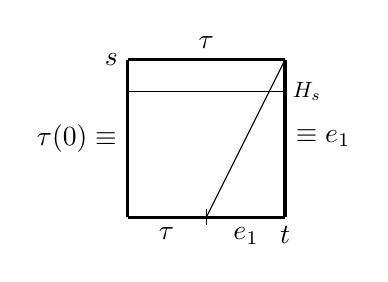
\begin{tikzpicture}[
				witharrow/.style={postaction={decorate}},
				vdot/.style={rectangle, fill, inner sep=0pt, outer sep=0pt, minimum width=0.5pt, minimum height=6pt}
				]
				
				\begin{scope}
				\draw[very thick]
				(0,0) coordinate (a1) -- node[left]{$\tau(0)\equiv$} (0,2) coordinate (d1)
				(2,0) coordinate (b1) -- node[right](q1){$\equiv e_1$} (2,2) coordinate (c1);
				
				\draw[very thick] (d1) -- node[above]{$\tau$} (2,2) coordinate (c1);
				
				\node[vdot] (b2) at (1,0) {};
				\draw[very thick] (a1) -- node[below]{$\tau$} (b2)
				(b2) -- node[below]{$e_1$} (b1);
				
				\draw[thin] (b2) -- (c1);
				
				\draw[very thin] (0, 1.6) -- (2,1.6) coordinate (h);
				\node[right, scale=0.8] at (h) {$H_s$};
				
				\node[below] at (b1) {$t$};
				\node[left] at (d1) {$s$};
				\end{scope}
				\end{tikzpicture}}
				
				\caption{Esquema de las homotopía para elementos neutros.}
			\end{figure}
		
			De nuevo, la intuición detrás de esta construcción es la misma. Es un buen ejercicio escribir las homotopías al detalle, y no lo haremos aquí. Además, el argumento de buena definición y continuidad es idéntico al del apartado anterior.
			
			\item En este caso, basta con demostrar que $\sigma\pathp\sigma' \homot e_0$ con extremos fijos, puesto que $\sigma=\sigma''$, y entonces aplicando el argumento a $\sigma'$ hemos terminado. Aunque la intuición geométrica es muy similar, la homotopía que resulta es algo distinta a los casos anteriores, y vamos a verla con algo más de detalle.
			
			Geométricamente, $\sigma'$ es $\sigma$ recorrido ``a la misma velocidad'', pero en sentido contrario. Entonces, $\sigma\pathp\sigma'$ va de $\sigma(0)$ a $\sigma(1)$ y vuelve por el mismo recorrido hasta $\sigma(0)$. Por tanto, la homotopía que vamos a considerar lo que hace es ``acercar cada vez más el punto donde se da la vuelta'', y esto en el extremo es una constante.
			
			\begin{figure}[h!]
				\label{grf_fig_homot_3}
				\centering
				\begin{tikzpicture}[
				decoration={markings,mark=at position 0.5 with {\arrow{>}}},
				witharrow/.style={postaction={decorate}},
				vdot/.style={rectangle, fill, inner sep=0pt, outer sep=0pt, minimum width=0.5pt, minimum height=6pt},
				dot/.style={draw,fill,circle,inner sep=1.5pt,minimum width=0pt, scale=0.45}
				]
				
				\begin{scope}
				\draw[very thick]
				(0,0) coordinate (a1) -- node[left]{$\sigma(0)\equiv$} (0,2) coordinate (d1)
				(2,0) coordinate (b1) -- node[right](q1){$\equiv\sigma'(1)$} (2,2) coordinate (c1);
				
				\draw[very thick] (d1) -- node[above]{$\sigma(0) = e_0$} (2,2) coordinate (c1);
				
				\node[vdot] (b3) at (1,0) {};
				\draw[very thick] (a1) -- node[below]{$\sigma$} (b3)
				(b3) -- node[below]{$\sigma\smash{'}$} (b1);
				
				\draw[thin] (b3) -- (d1);
				\draw[thin] (b3) -- (c1);
				
				\draw[very thin] (0, 1.5) -- (2,1.5) coordinate (h);
				\draw[thick] (0.25,1.5) coordinate (s1) -- (1.75,1.5) coordinate (s2);
				\node[dot] at (s1) {};
				\node[dot] at (s2) {};
				\node[above, scale=0.65] at (s1) {$\;\;\;\;\;\sigma(t)$};
				\node[above, scale=0.65] at (s2) {$\sigma(t)\;\;\;\;\;$};
				\node[right, scale=0.8] at (h) {$H_s$};
				
				\node[below] at (b1) {$t$};
				\node[left] at (d1) {$s$};
				\end{scope}
				\end{tikzpicture}
				
				\caption{Esquema de la homotopía entre $\sigma\pathp\sigma'$ y $e_0\equiv\sigma(0)$.}
			\end{figure}
		
			En este caso, la homotopía queda:
			\[H_s(t)=\left\{\begin{array}{ll}
			\sigma(2t) & \text{si } 0\leq t\leq\frac{1-s}{2} \\
			\sigma(1-s) & \text{si } \frac{1-s}{2}\leq t\leq\frac{1+s}{2} \\
			\sigma'(2t-1) & \text{si } \frac{1+s}{2}\leq t\leq 1
			\end{array}\right.\]
			y la prueba de que está bien definida y es homotopía coincide con la de los casos anteriores.
			
			\item En las condiciones del enunciado, supongamos que $H_s:\alpha\homot\sigma$ y $F_s:\beta\homot\tau$, ambas con extremos fijos. Entonces, podemos construir directamente la homotopía con extremos fijos $\alpha\pathp\beta\homot\sigma\pathp\tau$ como la siguiente:
			\[H_s(t)=\left\{\begin{array}{ll}
			H_s(2t) & \text{si } 0\leq t\leq\frac{1}{2} \\
			F_s(2t - 1) & \text{si } \frac{1}{2}\leq t\leq 0
			\end{array}\right.\]
			donde es interesante notar que se construye de forma muy similar al producto de dos caminos. Otra vez, la prueba de que está bien definida y es homotopía es la misma. \qedhere
		\end{enumerate}
	\end{proof}
\end{lem}

\section{Grupo fundamental}

Tras todas las preparaciones, por fin estamos en condiciones de afrontar el concepto que da nombre a este capítulo: el grupo fundamental.

No está de más recordar que $\X$ es, si no se dice lo contrario, conexo y localmente conexo por caminos.

\begin{defi}[Grupo fundamental]
	Sea $x_0\in\X$. Definimos el \tbi{grupo fundamental} de $\X$ con base $x_0$ como:
	\[\begin{split}
	\pi(\X,x_0) &= \left\{\text{lazos de base } x_0\right\} / {\homotef} \\
	&=\{\sigma:[0,1]\overset{\text{ cont.}}{\to}\X \mid \sigma(0)=\sigma(1)=x_0\} / {\homotef}
	\end{split}\]
	esto es, el conjunto de clases de homotopía de lazos, con la operación ${\pathp}$:
	\[\class{\sigma}\pathp\class{\tau} = \class{\sigma\pathp\tau}\]
\end{defi}

\begin{lem}
	El grupo fundamental está bien definido.
	
	\begin{proof}
	Hay que ver, primero, que la operación ${\pathp}$ está bien definida, y después que efectivamente es un grupo.
	
	Ya vimos en el lema \ref{grf_lema_prop_pathp} que la operación ${\pathp}$ respeta homotopía de extremos fijos, y por tanto la operacion ${\pathp}$ entre clases de equivalencia está bien definida.
	
	Entonces, solo queda ver que es un grupo. Hay que comprobar que es asociativa, que existe un elemento neutro y que todo elemento tiene inverso. Todas ellas se siguen de la propiedad correspondiente del lema \ref{grf_lema_prop_pathp}. Lo único que merece la pena comentar es que, en el caso del elemento neutro, el hecho de restringir los caminos a lazos con un punto base común garantiza la unicidad, y este elemento neutro es precisamente $x_0$.
	\end{proof}
\end{lem}

\begin{exa}[Grupos fundamentales]
	Presentamos ahora una serie de ejemplos de grupos fundamentales. Muchos de ellos los iremos demostrando a lo largo del texto, aunque habrá algunos que no lleguemos a ver por su complicación.
	
	Nótese que a menudo omitimos el punto base, porque, como veremos pronto, los grupos fundamentales para el mismo espacio respecto de distintos puntos base son isomorfos.
	
	\begin{enumerate}
		\item Dado $\X\subset\R^n$ estrellado, si tomamos como punto base el $x_0$ del ``centro'', ya vimos en el ejemplo \ref{grf_nulhomotopias_convexos} que todas las funciones son nulhomótopas, y entonces:
		\[\pi(\X,x_0)=\{1\}\]
		
		\item También vimos, en la proposición \ref{grf_homotop_caminos_esfera}, que $\pi(\Sfe^n)=\{1\}$ si $n\geq 2$.
		
		\item Para $n=1$, la circunferencia, resulta que $\pi(\Sfe^1)=\Z$.
		
		\item Un ejemplo de espacio con grupo fundamental finito no trivial es el espacio proyectivo real: $\pi(\proy^n)=\Z_2$.
		
		\item Como veremos más adelante, el producto de espacios tiene como grupo fundamental el producto de los grupos. Entonces, $\pi(\toro)=\pi(\Sfe^1)\times\pi(\Sfe^1)=\Z^2$.
		
		\item Para $\toro_g$, el toro con $g$ agujeros, tenemos que existe un homomorfismo de grupos sobreyectivo $\pi(\toro_g)\twoheadrightarrow \Z^2$. De hecho, en general, $\pi(\toro_g)$ ni siquiera es abeliano.
		
		\item El grupo fundamental del bouquet $B_n$, una figura geométrica generada pegando $n$ circunferencias, es $\pi(B_n)=\Z\pathp\overset{n}{\dots}\pathp\Z$, donde ${\pathp}$ denota el producto libre de grupos. Más adelante entraremos en detalle en este tema.
		
		\begin{figure}[h!]
			\centering
			\begin{tikzpicture}[scale = 0.4]
			\begin{polaraxis}[grid=none, axis lines=none]
			\addplot[mark=none,domain=0:360,samples=300] {cos(x*3)};
			\end{polaraxis}
			\end{tikzpicture}
			
			\caption{Un bouquet de tres pétalos.}
		\end{figure}
	
		\item $\pi(\Sfe^2\times\Sfe^2)=\{1\}$ y $\pi(\Sfe^4)=\{1\}$ pero $\Sfe^2\times\Sfe^2\centernot\homeo\Sfe^4$. Esto, que parece ser un contraejemplo a la versión generalizada para $n=4$ de la conjetura de Poincaré (\ref{grf_conjet_poincare}), no es tal; ya que para $n\geq 4$ se formula con condiciones adicionales. \qedhere
	\end{enumerate}
\end{exa}

\begin{prop}
	El grupo fundamental es independiente del punto base. Es decir, si $x_0,x_1\in\X$, entonces $\pi(\X,x_0)$ y $\pi(\X,x_1)$ son isomorfos.
	
	\begin{proof}
		Como asumimos que $\X$ es conexo por caminos, entonces existe un camino de $x_0$ a $x_1$ que llamamos $\alpha$. Así, definimos la siguiente función:
		\[\begin{split}
		f:\pi(\X,x_0) &\to \pi(\X,x_1) \\
		[\sigma]&\mapsto [\alpha'\pathp\sigma\pathp\alpha]
		\end{split}\]
		
		Y queremos comprobar que es isomorfismo de grupos:
		\begin{enumerate}
			\item Desde luego, está bien definida (si dos caminos son homótopos con extremos fijos, multiplicarlos por $\alpha$ y $\alpha'$ conserva la homotopía). Nótese que siguen siendo homótopos por extremos fijos pero los extremos en sí son otros.
			
			\item Es homomorfismo de grupos. En efecto, queremos ver que la imagen del producto es el producto de las imágenes. Entonces:
			\[f([\sigma]\pathp[\tau]) = f([\sigma\pathp\tau])=[\alpha'\pathp\sigma\pathp\tau\pathp\alpha]=[\alpha'\pathp\sigma\pathp\alpha\pathp\alpha'\pathp\tau\pathp\alpha] = [\alpha'\pathp\sigma\pathp\alpha]\pathp[\alpha'\pathp\tau\pathp\alpha]=f([\sigma])\pathp f([\tau])\]
			
			\item Es isomorfismo, porque su inversa es $[\lambda]\mapsto[\alpha\times\lambda\times\alpha']$ y esto es, por el apartado anterior, un homomorfismo. \qedhere
		\end{enumerate}
	\end{proof}
\end{prop}

\begin{obs}
	La proposición anterior parece dejar resuelto todo lo relativo al punto base: no solo nos garantiza que el grupo fundamental es independiente del punto base sino que además nos proporciona un isomorfismo explícito. Sin embargo, hay que tener cuidado con esto. Si pretendemos identificar todos los grupos fundamentales con uno solo, nos encontramos una dificultad: el isomorfismo depende del camino que escojamos. No hay una forma canónica de identificar uno por otro. 
	
	No es incorrecto hablar \ti{del} grupo fundamental de un espacio, pero siempre hay que tener en mente la consideración anterior. Como curiosidad, si el grupo fundamental es abeliano el isomorfismo sí es independiente del camino. 
\end{obs}

\begin{obs}
	Nótese que hemos necesitado que el espacio sea conexo por caminos para llevar a cabo la prueba anterior. Este es, de hecho, uno de los principales motivos por los que hemos restringido de tal forma el espacio $\X$.
\end{obs}

Para terminar la sección, definimos un concepto que nos ayudará a tratar con espacios con grupo fundamental trivial.

\begin{defi}[Simplemente conexo]
	Decimos que un espacio $\X$ conexo por caminos es \tbi{simplemente conexo} cuando su grupo fundamental es trivial.
\end{defi}

\section{\ti{General nonsense}. Funtorialidad}

El objetivo principal de esta sección es aplicar las ideas de teoría de categorías a los conceptos que hemos ido viendo a lo largo de este capítulo. Así, se recomienda leer antes el anexo \ref{funt}, que contiene una brevísima introducción a los conceptos más básicos de teoría de categorías. Esta no solo define los conceptos básicos como categoría o funtor sino que puede ayudar al lector a comprender el propósito detrás de este punto de vista, que a primera vista puede parecer terriblemente abstracto.

\begin{const}[Interpretación funtorial del grupo fundamental]
	En esta sección, vamos a considerar dos categorías. La primera de ellas es la \index[general]{categoría}categoría de espacios topológicos punteados \Topp, cuyos objetos son: 
	\[\{((\X,\T),x_0)\midc (\X,\T)\text{ espacio topológico}, x_0\in\X\}\]
	y en la cual los morfismos son las funciones continuas que preservan el punto base $x_0$. La segunda de ellas la categoría de los grupos \Grp, que tiene por objetos:
	\[\{(G,\cdot)\midc (G,\cdot) \text{ grupo}\}\]
	y por morfismos los homomorfismos de grupos.
	
	Entonces, consideramos tomar el grupo fundamental como un \index[general]{funtor}funtor. Es decir, consideramos el funtor $\pi$:
	\[\xymatrix @R=0.5pc @C=0.5pc {
		& & \Topp \ar[rrr]^\pi & & & \Grp & \\
		& & (\X,x_0) \ar@{|->}[rrr] \ar[dd]_{f \text{ cont.}} \ar@<1.5ex>@{|->}[dd] & & & \pi(\X,x_0) \ar[dd]_{f^\ast}^{\text{homom.}} \ar@{}[r]|-\ni & [\sigma] \ar@{|->}[dd] \\
		[0,1] \ar[urr]^\sigma \ar[drr]_{f\circ\sigma} & & & & & & \\
		& & (\Y,y_0) \ar@{|->}[rrr] & & & \pi(\Y,y_0) \ar@{}[r]|-\ni & [f\circ\sigma] \\
	}\]
	Nótese que denotamos $f^\ast$ al homomorfismo de grupos que es imagen de una aplicación continua $f$ por el funtor $\pi$.
	Como se aprecia en el diagrama, este homomorfismo $f^\ast$ se define, para una clase de equivalencia de caminos, de la siguiente forma:
	\[\begin{split}
	f^\ast:\pi(\X, x_0) &\to \pi(\Y, y_0) \\
	[\sigma] &\mapsto [f\circ\sigma]
	\end{split}\]
	Hay que comprobar, entonces, que está bien definido. En efecto, consideramos la aplicación $f^\ast$ que acabamos de definir. Desde luego, si $\sigma$ es un lazo con base $x_0$, $f\circ\sigma$ es un lazo con base $y_0$. Para ver si respeta la homotopía, consideramos $\tau:[0,1]\to (\X,x_0)$ homótopo con extremos fijos con $\sigma$ a través de la homotopía $H$. Entonces, $f\circ H$ es una homotopía entre $f\circ\sigma$ y $f\circ\tau$. Por último, comprobamos que es homomorfismo, lo cual es directo comprobando que $f\circ(\sigma\ast\tau)=(f\circ\sigma)\ast (f\circ\tau)$.
	
	Además, hay que ver que es un funtor, esto es, que cumple:
	\begin{itemize}
		\item $(g\circ f)^\ast = g^\ast\circ f^\ast$. En efecto, consideramos el lazo $\sigma$ con base en $x_0$. Sabemos que:
		\[(g\circ f)\circ\sigma=g\circ(f\circ\sigma)\]
		y tomando la imagen de $\sigma$ por $(g\circ f)^\ast$:
			\[(g\circ f)^\ast([\sigma])=[(g\circ f)\circ\sigma]=[g\circ(f\circ\sigma)]=g^\ast([f\circ\sigma])=g^\ast(f^\ast([\sigma]))=(g^\ast\circ f^\ast)([\sigma])\]
		como queríamos comprobar.
		
		\item $(\Id_\X)^\ast = \Id_{\pi(\X, x_0)}$. Esto se verifica directamente por como hemos definido $f^\ast$.
	\end{itemize}
\end{const}

Visto todo lo necesario, podemos pasar a comprobar una serie de propiedades utilizando el punto de vista introducido en la construcción anterior. La teoría de categorías es capaz a menudo de simplificar demostraciones al considerar los objetos abstractos, lo cual es una de sus grandes fortalezas. Vamos a ver ahora una serie de proposiciones que al mismo tiempo son ejemplos, pues muestran como enfocaríamos una demostración desde este nuevo punto de vista. Sin embargo, no dejan de ser resultados interesantes por sí mismos.

\begin{prop}
	El funtor grupo fundamental manda homeomorfismos en isomorfismos de grupos. En particular, si dos espacios tienen distinto grupo fundamental, entonces no son homeomorfos.
	
	\begin{proof}
		Sean $\X,\Y$ dos espacios topológicos punteados con $x_0$, $y_0$, y $f$ un homeomorfismo entre ellos de forma que:
		\[\xymatrix @R=0.4pc {
			\X \ar[r]^f_{\text{homeo.}} & \Y \ar[r]^{g=f^{-1}} & \X \\
			x_0 \ar@{|->}[r] & y_0 \ar@{|->}[r] & x_0
		}\]
		
		Ahora, tenemos que:
		\[g^\ast\circ f^\ast = (g\circ f)^\ast = (\Id_\X)^\ast = \Id_{\pi(X)}\]
		\[f^\ast\circ g^\ast = (f\circ g)^\ast = (\Id_\Y)^\ast = \Id_{\pi(Y)}\]
		y con esto hemos comprobado que $g^\ast$ es la inversa de $f^\ast$, luego $f^\ast$ es isomorfismo.
	\end{proof}
\end{prop}

\begin{prop}
	\label{grf_prop_retractos_homo_sobreyectivo}
	Un \index[general]{retracto}retracto, como veremos con detalle más adelante, es un subespacio tal que existe una aplicación continua que deforma el espacio en él, como se aprecia en el siguiente esquema:
	\[\xymatrix @C=0.65pc {
		A \ar@{}[r]|\subset \ar[dr]_{\rho\restriction_A = \Id} & \X \ar[d]^{\rho\text{ retracto}} \\
		& A
	}\]
	Entonces, la imagen $\rho^\ast$ de $\rho$ por $\pi$ es un homomorfismo sobreyectivo. En particular, si el grupo fundamental del retracto $A$ es no trivial, entonces el grupo fundamental del espacio $\X$ tampoco es trivial.
	
	\begin{proof}
		Para la demostración, consideramos la imagen por $\pi$ del diagrama anterior, donde $A$ y $\X$ tienen el mismo punto base $x_0\in A$:
		\[\xymatrix {
			\pi(A,x_0) \ar[r]^{j^\ast} \ar[dr]_{(\rho\restriction_A)^\ast = \Id_{\pi(A)}} & \pi(\X,x_0) \ar[d]^{\rho^\ast} \\
			& \pi(A,x_0)
		}\]
		donde $j$ es la aplicación inclusión de $A$ en $\X$. Como por las propiedades de los funtores $\rho^\ast\circ j^\ast=(\rho\circ j)^\ast$, el diagrama anterior conmuta, es decir:
		\[\rho^\ast\circ j^\ast=\Id_{\pi(A)}\]
		
		Ahora, como $\Id_{\pi(A)}$ es biyectivo, y en particular sobreyectivo, $\rho^\ast\circ j^\ast$ también debe ser sobreyectivo, y entonces necesariamente $\rho^\ast$ lo es.
	\end{proof}
\end{prop}

Un caso donde se puede aplicar la proposición anterior es el siguiente.

\begin{exa}
	Consideramos el disco cerrado $\adher{D}_2\subset\R^2$. Queremos comprobar que el disco no se puede retraer a $A=\Sfe^1=\partial\adher{D}_2$. Como veremos más adelante, $\pi(A)=\pi(\Sfe^1)=\Z$, y ya sabemos que $\pi(\adher{D}_2)=\{1\}$, pues es un estrellado en $\R^n$. Entonces, si fuera retracto, habría un homomorfismo sobreyectivo del grupo trivial a $\Z$, y esto es imposible.
\end{exa}

\begin{prop}
	\label{grf_prop_gf_prod_es_prod_gf}
	Dados dos espacios $\X,\Y$, el grupo fundamental del producto es isomorfo al producto de los grupos fundamentales. Esto es:
	\[\pi(\X\times\Y)\approx\pi(\X)\times\pi(\Y)\]
	
	\begin{proof}
		Consideramos los puntos base $x_0,y_0$ respectivamente. El esquema de la topología producto sería el siguiente:
		\[\xymatrix @R = 0.4pc{
			& \X & \\
			\X\times\Y \ar[ur]^p \ar[dr]_q & & [0,1] \ar[ul]^\sigma \ar[dl]^\tau \\
			& \Y &
		}\]
		donde $p$ y $q$ son las proyecciones. Entonces, como ya hemos hecho antes, vamos a ver la imagen de este diagrama:
		\[\xymatrix @R = 0.4pc @C = 0.5pc {
			& \pi(\X) & & & *+[r]{[p\circ (\sigma,\tau)]=[\sigma]} \\
			\pi(\X,\Y)  \ar[ru]^{p^\ast} \ar[rd]_{q^\ast} \ar[rr]^-{(p^\ast,q^\ast)} & & \pi(\X)\times\pi(\Y) \ar@{}[r]|-\colon& [(\sigma,\tau)] \ar@{|->}[ru] \ar@{|->}[rd] \ar@{|->}[r] & ([\sigma],[\tau]) \\
			& \pi(\Y) & & & *+[r]{[q\circ (\sigma,\tau)]=[\tau]}
		}\]
		
		Nótese que hemos añadido la aplicación que llega a $\pi(\X)\times\pi(\Y)$. Si comprobamos que es un isomorfismo, entonces tenemos lo que estábamos buscando. En efecto:
		\begin{itemize}
			\item Es trivialmente sobreyectivo.
			\item Es inyectivo. Para verlo, usaremos un resultado conocido que afirma que un homomorfismo es inyectivo si y solo si su núcleo es trivial. Entonces, denotando $e_X$ al elemento identidad de cada grupo $\pi(X)$, sean $\sigma,\tau$ de forma que $([\sigma],[\tau])=(e_\X,e_\Y)$. Queremos ver que necesariamente $[(\sigma,\tau)]=e_{\X\times \Y}$.
			
			Consideramos las homotopías $K_s:\sigma\homot x_0=e_\X$, $L_s:\tau\homot y_0=e_\Y$. Entonces, $(K_s,L_s):(\sigma,\tau)\homot(x_0,y_0)=e_{\X\times\Y}$ es homotopía y, por tanto, el núcleo del homomorfismo es $\{e_{\X\times\Y}\}$.
		\end{itemize}
		Por tanto, es isomorfismo.
	\end{proof}
\end{prop}

Un ejemplo de la utilidad de este resultado es el siguiente.

\begin{exa}
	Consideramos el toro $\toro$, que sabemos que es homeomorfo a $\Sfe^1\times\Sfe^1$. Entonces, cuando veamos más adelante que $\pi(\Sfe^1)=\Z$, podremos afirmar directamente que $\pi(\toro)=\Z\times\Z$.
\end{exa}

\section{Espacios recubridores. El problema de elevación}

El estudio de los espacios recubridores de otro espacio es a menudo útil para calcular grupos fundamentales, y en general tiene una gran relación con el estudio de ellos. En esta sección planteamos el problema de elevación en su versión más general, para luego particularizarlo para poder demostrar propiedades útiles.

\subsection{Espacios recubridores}

Para empezar, vamos a formalizar el concepto de espacio recubridor.

\begin{defi}[Espacio recubridor]
	Sea $p:\widetilde{\X}\to \X$ una aplicación continua y sobreyectiva. Decimos que $\widetilde{\X}$ es un \tbi[espacio!recubridor]{espacio recubridor} de $X$ si para cada $x\in\X$ existe un entorno $U_x$ que verifica que $p^{-1}(U_x)$ se puede escribir como unión disjunta de conjuntos $U_\lambda$ donde cada uno de ellos es homeomorfo a $U_x$, de forma que, para cada $\lambda$, $p\restriction_{U_\lambda}:U_\lambda\to U_x$ sea un homeomorfismo.
\end{defi}

\begin{exa}[Recubrimientos]
	\label{grf_exa_recubrimientos}
	Veamos algunos ejemplos de espacios recubridores.
	
	\begin{enumerate}
		\item $\Sfe^n$ recubre al plano proyectivo real $\proy^n$, con la siguiente aplicación:
		\[\begin{split}
		p:\Sfe^n&\to\proy^n \\
		(x_0,\dots,x_n)&\mapsto (x_0:\dotsc:x_n)
		\end{split}\]
		En efecto, tomamos un punto $(x_0:\dotsc:x_n)\in\proy^n$. Tomando un entorno abierto del punto, homeomorfo a un disco, su imagen inversa consiste en dos abiertos homeomorfos a discos alrededor de dos puntos antipodales de $\Sfe^n$. Estos son disjuntos y se verifican las condiciones.
		
		\item $\R$ recubre al círculo $\Sfe^1$, con la aplicación:
		\[\begin{split}
		p:\R&\to\Sfe^1 \\
		t &\mapsto e^{2\pi t}=(\cos 2\pi t,\sin 2\pi t)
		\end{split}\]
		En efecto, para un punto $x$ del círculo, tomamos un entorno abierto: un arco que lo contenga sin extremos. Esto es homeomorfo a un intervalo abierto, y su imagen inversa consiste en una cantidad numerable de intervalos a lo largo de la recta real, cada uno conteniendo un punto de $p^{-1}(x) = \Z + a$ para algún $a\in\R$. Como, tomando el entorno inicial lo suficientemente pequeño, todos estos intervalos son disjuntos, ya está. \qedhere
	\end{enumerate}
\end{exa}

\subsection{El problema de elevación}

Con esto, estamos ya en condiciones de formular el problema de elevación.

\begin{const}[Formulación del problema de elevación]
	\index[general]{problema de elevación}
	Consideramos el diagrama:
	\[\xymatrix{
		& \widetilde{\X} \ar[d]^p \\
		\mc{Z} \ar@{-->}[ru]^{\widetilde{H}} \ar[r]^H & \X
	}\]
	
	Aquí, $\widetilde{\X}$ es un espacio recubridor mediante la aplicación $p$. El problema de elevación pregunta por la existencia de la aplicación del diagrama $\widetilde{H}:\mc{Z}\to \widetilde{X}$, continua y que verifique que $p\circ\widetilde{H}=H$, es decir, que haga que el diagrama sea conmutativo. Una aplicación que verifique esto se llama \tbi{elevación}.
\end{const}

\begin{lem}[Existencia de elevación local]
	\label{grf_lema_elevacion_local}
	Sea $z_0\in\mc{Z}$, $x_0=H(z_0)\in U$ abierto de $\X$. Entonces, para un único $\lambda$, existe una elevación local $\widetilde{H}$ que muere en $U_\lambda$ de forma que el siguiente esquema es conmutativo:
	\[\xymatrix{
		& U_\lambda \ar[d]^{p\restriction_{U_\lambda}} \\
		\mc{Z}\supset H^{-1}(U) \ar[ru]^-{\widetilde{H}} \ar[r]^-H & U
	}\]

	Además, $\widetilde{H}=(p\restriction_{U_\lambda})^{-1}\circ H$.
	
	\begin{proof}
		Basta con comprobar que $\widetilde{H}=(p\restriction_{U_\lambda})^{-1}\circ H$ es una elevación, bien definida, que muere en $U_\lambda$. 
		
		Ahora, para ver que es elevación, basta con darse cuenta de que $p\restriction_{U_\lambda}$ es un homeomorfismo por definición de espacio recubridor. Entonces, no solo está bien definida (por existir la inversa de $p\restriction_{U_\lambda}$), sino que además la composición $\widetilde{H} = (p\restriction_{U_\lambda})^{-1}\circ H$ es continua y como, desde luego, hace conmutativo el diagrama, es elevación.
		
		Para ver que, en efecto, muere en $U_\lambda$, usamos que $\widetilde{H}(x_0)\in p^{-1}(x_0)$, pues $p\widetilde{H}(z_0)=H(z_0)=x_0$. Entonces, consideramos:
		\[\widetilde{H}(z_0)\in p^{-1}(x_0)\subset p^{-1}(U)=\bigcup_\lambda U_\lambda\]
		y como la unión es disjunta, existe un único $\lambda$ de forma que $\widetilde{H}(z_0)\in U_\lambda$.
	\end{proof}
\end{lem}

\begin{lem}[Unicidad de la elevación]
	\label{grf_lema_unicidad_elevacion}
	Si, para un $\mc{Z}$ conexo, dos elevaciones coinciden en un punto, entonces son la misma.
	
	\begin{proof}
		Consideramos dos elevaciones $\Phi$ y $\Psi$ que cumplan las condiciones anteriores. Queremos ver que ambas son la misma. Como $\mc{Z}$ es conexo, podemos comprobar que $\{\Phi(z)=\Psi(z)\}$, que es no vacío (porque, por hipótesis, coinciden en un punto), es abierto y cerrado en $\mc{Z}$.
		
		\begin{itemize}
			\item Veamos que es abierto. Sea $z\in\mc{Z}$, entonces existe un entorno $W$ de $z$ tal que $\Phi\restriction_{W}=(p\restriction_{U_\lambda})^{-1}\circ H$, y existe otro entorno $W'$ de $z$ tal que $\Psi\restriction_{W'}=(p\restriction_{U_\lambda})^{-1}\circ H$; con $\Phi(z)\in U_\lambda$ y $\Psi(z)\in U_\mu$. Como $\Phi(z)=\Psi(z)$, $U_\lambda = U_\mu$ (por ser la unión disjunta). Entonces $\Phi\restriction_{W\cap W'}=\Psi\restriction_{W\cap W'}$, y por tanto $W\cap W'\subset\{\Phi(z)=\Psi(z)\}$, y es entorno, luego este es abierto.
			
			\item Vamos a ver que el complementario $\{\Phi(z)\neq\Psi(z)\}$ es abierto. Primero, $\lambda\neq\mu$. En efecto, si estuvieran en el mismo $U_\lambda$, $p\Phi(z)\neq p\Psi(z)$, pero por ser elevaciones ambos son iguales a $H(z)$, lo cual es una contradicción. Entonces, si $\lambda\neq\mu$, definiendo $W$ y $W'$ como en el apartado anterior, $\Phi(W\cap W')\cap \Psi(W\cap W')\subset U_\lambda\cap U_\mu=\emptyset$. Entonces, $W\cap W'\subset \{\Phi(z)\neq\Psi(z)\}$, luego este es abierto. \qedhere
		\end{itemize}
	\end{proof}
\end{lem}

El lema que sigue tiene una importancia capital a la hora de demostrar cuál es el grupo fundamental de muchos espacios.

\begin{lem}[De elevación de homotopías]
	\label{grf_lema_elevacion_homotopias}
	Dada una homotopía $H:\mc{Z}=\Y\times [0,1]\to\X$ y una elevación $\widetilde{f}$ de $f=H_0:\Y\to\X$, entonces existe una única elevación $\widetilde{H}$ de $H$ tal que $(\widetilde{H})_0=\widetilde{f}$.
	
	\begin{proof}
		Nótese que no tenemos que preocuparnos de la unicidad: ya la demostramos en el lema \ref{grf_lema_unicidad_elevacion}. Será más complicado probar la existencia.
		
		La demostración de la existencia tiene dos pasos. Primero, trataremos de construir una elevación semilocal para luego intentar pegar todos estos ``trozos'' de elevación, construyendo así la elevación global. Recordamos de nuevo que estamos intentando construir una elevación que haga conmutativo el diagrama:
		\[\xymatrix{
			& \widetilde{\X} \ar[d]^p \\
			\Y\times [0,1] \ar@{-->}[ru]^{\widetilde{H}} \ar[r]^-H & \X
		}\]
		y que además verifique que $(\widetilde{H})_0=\widetilde{f}$.
		
		Vamos a construir, pues, lo que hemos llamado una elevación semilocal, es decir, para cada $y\in\Y$ una elevación $\widetilde{H}_y:V_y\times [0,1]\to\widetilde{X}$, donde $V_y$ es un entorno abierto de $\Y$.
		
		De esta forma, fijando $y\in \Y$, consideramos la restricción de $H$:
		\[\{y\}\times [0,1]\overset{H}{\to}X=\bigcup_x U_x\]
		Ahora, aplicamos el lema de Lebesgue (\ref{comp_lem_lebesgue}), considerando el recubrimiento abierto $H^{-1}(U_{x_i})$. Entonces, existe una partición $0=t_0<t_1<\dots<t_r=1$ de forma que $\{y\}\times [t_{i-1}, t_i]\subset H^{-1}(U_{x_i})\subset \Y\times [0,1]$ para ciertos $x_i$. Aplicando el conocido lema de Wallace (que no hemos demostrado aquí), como $H^{-1}(U_{x_i})$ es un abierto en el compacto $\Y\times [0,1]$, y $\{y\}\times [t_{i-1},t_i]$ es un compacto en ese abierto, entonces existe un entorno $V_y^i$ de forma que $V_y^i\times [t_{i-1},t_i]\subset H^{-1}(U_{x_i})$. Entonces, definimos $V_y=\bigcap_{j=1}^r V_y^j$ entorno abierto de $y$.
		
		Con el entorno definido de esta forma, vamos a fabricar la elevación $\widetilde{H}_y$ de $H\restriction_{V_y\times [0,1]}$. Para ello, vamos a considerar, para cada $i$, la restricción $H:V_y^i\times [t_{i-1},t_i]\to U_{x_i}$. Procedemos por inducción sobre los $\{t_0,\dots, t_r\}$ de la partición:
		
		\begin{itemize}
			\item El caso base es simplemente la homotopía:
			\[\widetilde{H}_y\restriction_{V_y\times\{0\}}=\widetilde{f}\restriction_{V_y}\]
			
			\item Para el paso inductivo, supongamos dada $\widetilde{H}_y\restriction_{V_y\times [0,t_i]}$. Como se cumple que la homotopía $H\restriction_{V_y\times [t_i,t_{i+1}]}$ acaba en $U^{x_{i+1}}$, resulta que $H(y,t_i)\in U_{x_{i+1}}$. Entonces, se cumple:
			\[\widetilde{H}^y(y, t_i)\in p^{-1}(U^x_{i+1})=\bigcup_\lambda U_\lambda^{x_{i+1}}\]
			donde la unión es disjunta. De esta forma, existe un (único) $\lambda$ tal que $\widetilde{H}_y(y, t_i)\in U_\lambda^{x_{i+1}}$. Así, $(y,t_i)\in (\widetilde{H}_y)^{-1}(U_\lambda^{x_{i+1}})$, que es abierto, y por tanto existe un entorno $W_y$ que cumple que $W_y\times \{t_i\}\subset (\widetilde{H}_y)^{-1}(U_\lambda^{x_{i+1}})$. Reducimos entonces el entorno original $V_y$ a $V_y\cap W_y$, que desde luego es entorno por ser intersección de entornos, y entonces $V_y\times\{t_i\}\subset (\widetilde{H}_y)^{-1}(U_\lambda^{x_{i+1}})$.
			
			Ahora, por el lema \ref{grf_lema_elevacion_local} de elevación local, ya que tenemos que:
			\[V_y\times [t_i, t_{i+1}]\subset H^{-1} U^{x_{i+1}}\]
			podemos encontrar una elevación:
			\[\widetilde{H}_y\restriction_{V_y\times [t_i,t_{i+1}]} = (p\restriction_{U_\lambda^{x_{i+1}}})^{-1}\circ H \]
			
			Con lo anterior, solo necesitamos comprobar que la aplicación:
			\[\widetilde{H}_y\restriction_{V_y\times [0,t_{i+1}]} = \left\{\begin{array}{ll}
			\widetilde{H}_y\restriction_{V_y\times [0,t_i]} & \text{si } 0\leq t \leq t_i \\
			\widetilde{H}_y\restriction_{V_y\times [t_i,t_{i+1}]} & \text{si } t_i\leq t \leq t_{i+1} \\
			\end{array}\right.\]
			está bien definida, es continua y es elevación. 
			
			Que está bien definida se ve rápidamente a partir de las comprobaciones anteriores. En efecto, hay que comprobar que el valor de cada trozo en $V_y\times\{t_i\}$ coincide. Para ello, usaremos que ambas son elevaciones de $H$, de forma que, para cualquier $y'\in V_y$:
			\[p\restriction_{U_\lambda^{x_{i+1}}}(\widetilde{H}_y\restriction_{[0,t_i]}(y',t_i)) = H(y',t_i) = p\restriction_{U_\lambda^{x_{i+1}}}(\widetilde{H}_y\restriction_{[t_i,t_{i+1}]}(y',t_i)) \]
			y por ser $p\restriction_{U_\lambda^{x_{i+1}}}$ homeomorfismo son iguales.
			
			La continuidad es directa por existir un recubrimiento cerrado tal que la restricción es continua en cada parte (los propios trozos). Y que es elevación se comprueba directamente.
		\end{itemize}
	
		Con esta inducción, hemos generado, para cada $y\in\Y$, una elevación $\widetilde{H}_y:V_y\times [0,1]\to\widetilde{X}$. Ahora, pasamos a ver que se pueden ``pegar'' todas estas elevaciones para construir una elevación global. 
		
		Consideramos pues dos puntos $y,y'\in\Y$ y las elevaciones correspondientes $\widetilde{H}_y$ y $\widetilde{H}_{y'}$. Basta comprobar que ambas coinciden el la parte común de los dominios: $V_y\cap V_{y'}$.
		
		Para probar esto, consideramos $y''\in V_y\cap V_{y'}$. Queremos comprobar que $\widetilde{H}_y(y'',\cdot)=\widetilde{H}_{y'}(y'',\cdot)$. Pero ambas son elevaciones de $H$ en $\{y''\}\times [0,1]$ y entonces ambas deben cumplir:
		\[\widetilde{H}_y(y'',0)=\widetilde{f}(y'')=\widetilde{H}_{y'}(y'',0)\]
		
		Entonces, como coinciden en un punto de un conexo ($\{y''\}\times [0,1]$), ya vimos en el lema \ref{grf_lema_unicidad_elevacion} que coinciden. 
	\end{proof}
\end{lem}

El siguiente resultado bien podría llamarse corolario, pues es un caso particular del lema de elevación de homotopías, pero dada la importancia que tiene lo consideramos un lema en sí mismo.

\begin{lem}[De elevación de caminos]
	\label{grf_lema_elevacion_caminos}
	Dado un camino $\sigma:\mc{Z}= [0,1]\to\X$, de origen $x_0\in\X$, entonces existe una única elevación $\widetilde{\sigma}$ de $\sigma$ tal que el origen de $\widetilde{\sigma}$ sea $\widetilde{x_0}\in\widetilde{X}$.
	
	\begin{proof}
		Si en el lema de elevación de homotopías tomamos $\Y=\{a\}$, y consideramos la función $\widetilde{f}:\Y\to \widetilde{\X}$ tal que $\widetilde{f}(a)=\widetilde{x_0}$, tenemos el resultado.
	\end{proof}
\end{lem}

\begin{obs}
	La elevación es un problema homotópico. En efecto, si $f:\Y\to\X$ tiene una elevación $\widetilde{f}:\Y\to\widetilde{\X}$, entonces toda $g\homot f$ tiene también elevación.  Basta con considerar la homotopía $H:f\homot g$, y por el lema de elevación existe $\widetilde{H}$, de forma que $\widetilde{g} = \widetilde{H}_1$ eleva a $g$.
\end{obs}

\section{El grupo fundamental del espacio proyectivo}

El objetivo de esta sección es calcular el grupo fundamental de $\proy^n$, el espacio proyectivo real de dimensión $n$, para $n\geq 2$. Como pronto veremos, esta demostración explota el concepto de elevación. 

\begin{theo}[Grupo fundamental de $\proy^n$]
	\label{grf_espacio_proyectivo}
	
	Para $n\geq 2$, el grupo fundamental de \indexg{espacio proyectivo} $\proy^n$ es $\pi(\proy^2)=\Z_2$, el grupo abeliano de orden 2.
	
	\begin{proof}
		Vamos a empezar demostrando que la esfera $\Sfe^n$ es un espacio recubridor del espacio proyectivo $\proy^n$. Vamos a repetir con un poco más de detalle el argumento que ya utilizamos en el ejemplo \ref{grf_exa_recubrimientos}. Consideramos pues la aplicación:
		\[\begin{split}
		p:\Sfe^n&\to\proy^n \\
		(x_0,\dots,x_n)&\mapsto (x_0,\dotsc,x_n)
		\end{split}\]
		Entonces, sea un punto $y\in\proy^n$. Tenemos que comprobar que para cada $x\in p^{-1}(y)$ existe un entorno $U_x$ tal que $p^{-1}(U_x)$ es union disjunta de conjuntos $U_\lambda$, donde cada $U_\lambda\homeo U_x$.
		
		De esta forma, para $y\in\proy^n$, consideramos un hiperplano $\pi$ que no lo contenga. Como el plano $\pi$ es cerrado, $U=\proy^n\setminus\pi$ es abierto, y además contiene a $x$, luego es entorno. La imagen inversa del plano $\pi$ es, para la misma aplicación definida en todo $\R^{n+1}$, un hiperplano; y de esta manera la imagen inversa de $\proy^n\setminus\pi$ por $p:\Sfe^n\to\proy^n$ son dos casquetes de la esfera. Llamamos pues a estos $U_+$, $U_-$ y desde luego son abiertos. Como la imagen inversa de $x$ son dos puntos antipodales, que llamamos $p$ y $-p$, y no están en $p^{-1}(\pi)$, entonces está cada uno en un casquete. De esta forma, como los casquetes son entornos disjuntos, basta con comprobar que $U_+,U_-\homeo U_x$. Pero resulta que $U_x = \proy^n\setminus\pi\homeo\R^n$, y $U_+,U_-\homeo\R^n$ porque son homeomorfos a discos abiertos.
		
		Visto esto, planteamos la siguiente elevación de caminos. Sea $a=(1:0:\dotsc:0)$ el punto base del grupo fundamental. Entonces, tenemos el diagrama:
		\[\xymatrix @C = 0.5pc {
			&& \Sfe^n \ar[d]^p & (x_0,\dots,x_n) \ar@{|->}[d] \ar@{}[l]|-\ni \\
			[0,1] \ar[rr]^\sigma \ar[rru]^{\widetilde{\sigma}} && \proy^n & (x_0,\dotsc,x_n) \ar@{}[l]|-\ni
		}\]
		de forma que $\sigma$ es un lazo en $\proy^n$ con base en $a$, y por tanto verifica $\sigma(0)=\sigma(1)=a$. Si llamamos $p^{-1}(a)=\{\widetilde{a},-\widetilde{a}\}$, por el lema de elevación de caminos (\ref{grf_lema_elevacion_caminos}), podemos elegir $\widetilde{\sigma}$ de forma que se verifique que $\widetilde{\sigma}(0)=\widetilde{a}$. Pero como tan solo sabemos que $p\circ\widetilde{\sigma}=\sigma$, entonces $\widetilde{\sigma}(1)$ no tiene por qué ser $\widetilde{a}$, puede ser también $-\widetilde{a}$.
		
		Planteamos entonces dos casos:
		\begin{enumerate}[label=\roman*)]
			\item $\widetilde{\sigma}$ es un lazo en $\Sfe^n$ de base $\widetilde{a}$. Como ya vimos en la proposición \ref{grf_homotop_caminos_esfera} que $\pi(\Sfe^n)=\{1\}$, podemos escribir:
			\[\widetilde{H}_s:\widetilde{\sigma}\homot\widetilde{e}=\widetilde{a}\]
			y tomando imágenes por $p$ tenemos:
			\[H_s=p\circ\widetilde{H}_s:p\circ\widetilde{\sigma}\homot p\circ\widetilde{e}\]
			y por ser $p\circ\widetilde{\sigma}=\sigma$, tenemos que $H_s: \sigma\homot e=a$. Por tanto, $[\sigma] = 1\in\pi(\proy^n,a)$.
			
			\item $\widetilde{\sigma}$ es un camino en $\Sfe^n$ de $\widetilde{a}$ a $-\widetilde{a}$. Consideramos el camino:
			\[\widetilde{\alpha}(t)= (\cos\pi t, \sen\pi t,0,\dots, 0) \]
			que verifica que $\widetilde{\alpha}(0)=\widetilde{a}$ y $\widetilde{\alpha}(1)=-\widetilde{a}$. De nuevo, por estar en $\Sfe^n$ existe una homotopía con extremos fijos:
			\[\widetilde{H}_s:\widetilde{\sigma}\homot[\widetilde{a},-\widetilde{a}]\widetilde{\alpha}\]
			y, de nuevo tomando imágenes, obtenemos la homotopía:
			\[p\circ H_s:\sigma\homot\alpha\]
			donde los extremos fijos son $p(\widetilde{a}),p(-\widetilde{a})$, y ambos son $a$. Por tanto es homotopía de lazos. Entonces, tenemos que $[\sigma] = [\alpha]\in\pi(\proy^n,a)$.
		\end{enumerate}
		
		De esta forma, hemos comprobado que cualquier lazo de $\proy^n$ está en alguna de las dos clases de homotopía. Con ello, podemos asegurar que $\card{\pi(\proy^n,a)}\leq 2$. Veamos pues que las clases $1$ y $[\alpha]$ son distintas.
		
		En efecto, si fueran iguales consideramos la homotopía $H_s:\alpha\homot[a] e$. Esta verifica $H_s(0)=H_s(1)\equiv a$, $H_0=\alpha$ y $H_1\equiv a$. Al elevarla, nos queda un diagrama como el siguiente:
%		\[\xymatrix{
%			& \Sfe^n \ar[d]^p \\
%			[0,1]\times[0,1] \ar[r]^-H \ar[ru]^{\widetilde{H}} & \proy^n
%		}\]
		\[\xymatrix{
			& \Sfe^n \ar[d]^p \\
			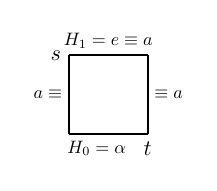
\begin{tikzpicture}[baseline=-0.5ex,
			scale=0.5,
			vdot/.style={rectangle, fill, inner sep=0pt, outer sep=0pt, minimum width=0.5pt, minimum height=6pt},
			dot/.style={draw,fill,circle,inner sep=1.5pt,minimum width=0pt, scale=0.45}
			]
			\draw[thick]
			(0,0) coordinate (a1) -- node[left,scale=0.65]{$a\equiv$} (0,2) coordinate (d1)
			(2,0) coordinate (b1) -- node[right,scale=0.65](q1){$\equiv a$} (2,2) coordinate (c1);
			\draw[thick] (d1) -- node[above,scale=0.65] {$H_1=e\equiv a$} (2,2) coordinate (c1);
			\draw[thick] (a1) -- node[below,scale=0.65] {$H_0=\alpha\quad\;$} (b1);
			\node[below,scale=0.8] at (b1) {$t$};
			\node[left,scale=0.8] at (d1) {$s$};
			\end{tikzpicture} \ar[r]^-H \ar[ru]^-{\widetilde{H}} & \proy^n
		}\]
		
		donde la existencia de $\widetilde{H}$ está garantizada por el lema de elevación (\ref{grf_lema_elevacion_caminos}). 
		
		Ahora, considerando el subconjunto $Z$ formado por los tres lados superiores de $[0,1]\times [0,1]$, tenemos que $\widetilde{H}$ eleva a $e\equiv a$ (en efecto, $p\widetilde{H}=a$). Sin embargo, podemos considerar también la homotopía $\widetilde{H}'=\widetilde{a}$, que es constantemente $\widetilde{a}$. Esta también eleva en $Z$ a $e\equiv a$. Además, coinciden en un punto, pues:
		\[\widetilde{H}_0(0)=\widetilde{\alpha}(0)=\widetilde{a}\]
		y entonces, por la unicidad de la elevación (lema \ref{grf_lema_unicidad_elevacion}), tenemos que $\widetilde{H}=\widetilde{e}$ en $Z$. Pero entonces:
		\[\widetilde{H}_0(1) = \widetilde{\alpha}(1) = \widetilde{e} = \widetilde{a}\]
		pero esto claramente no ocurre por definición de $\widetilde{\alpha}$, luego ya tenemos nuestra contradicción.
		
		Entonces, el grupo fundamental de $\proy^n$ tiene dos elementos, y por tanto tiene que ser $\Z_2$.
	\end{proof}
\end{theo}

\section{El grupo fundamental del círculo}

El objetivo de esta sección es calcular el grupo fundamental de $\Sfe^1$, el círculo de $\R^2$. Además, este es homeomorfo a $\proy^1$, la recta proyectiva real, con lo que, considerando también la sección anterior, ya tendremos el grupo fundamental del espacio proyectivo de cualquier dimensión.

\begin{theo}[Grupo fundamental de $\Sfe^1$]
\label{grf_circulo}

El grupo fundamental de $\Sfe^1$ es $\pi(\Sfe^1)=\Z$.

\begin{proof}
Consideramos el siguiente esquema:
\[\xymatrix @C = 0.5pc {
&&\R \ar[d]^p & t \ar@{|->}[d] \\
[0,1] \ar[rr]^\sigma \ar[rru]^{\widetilde{\sigma}} & & \Sfe^1 & e^{2\pi ti}
}\]
donde ya hemos visto que $\R$ es un espacio recubridor con la aplicación $p$.

Definimos entonces la siguiente aplicación entre grupos:
\[\begin{split}
\indice:\pi(\Sfe^1,a)&\to\Z \\
[\sigma] &\mapsto \indice\sigma = \widetilde{\sigma}(1)-\widetilde{\sigma}(0)
\end{split}\]
para cualquier elevación $\widetilde{\sigma}$ de $\sigma$ en $\R$. La denominamos \tbi[indice@índice]{índice}, \tbi[numero de vueltas@número de vueltas|see{índice}]{número de vueltas} o \tbi[grado|see{índice}]{grado}.

El objetivo de la demostración es comprobar que la aplicación $\indice$ anterior es un isomorfismo de grupos, pues entonces hemos terminado. Desde luego, es necesario comprobar también que está bien definida.

En primer lugar, comprobamos que $\indice$ no depende de la elevación $\widetilde{\sigma}$. Para ello, sea $\widehat{\sigma}$ otra elevación. Tenemos que verificar que $\widetilde{\sigma}(1)-\widetilde{\sigma}(0) = \widehat{\sigma}(1) - \widehat{\sigma}(0)$. Consideramos entonces la aplicación:
\[[0,1]\ni t\mapsto \widetilde{\sigma}(t) - \widehat{\sigma}(t)\]
Como $p\circ\widetilde{\sigma} = p\circ\widehat{\sigma} = \sigma$, necesariamente $\widetilde{\sigma}(t) - \widehat{\sigma}(t)\in\Z$. Dado que la aplicación anterior es continua y $[0,1]$ es conexo, su imagen es conexa, y un conexo en $\Z$ es un punto, es decir, $\widetilde{\sigma}(t) - \widehat{\sigma}(t)$ es constante, y la llamamos $k$. Entonces:
\[\widetilde{\sigma}(1)-\widetilde{\sigma}(0) = (\widehat{\sigma}(1) + k) - (\widehat{\sigma}(0) + k) = \widehat{\sigma}(1) - \widehat{\sigma}(0)\]

Para asegurar que está bien definida, también hace falta ver que $\indice$ no depende del representante. Es decir, que dados $\sigma,\tau$ de forma que $\sigma\homot[a]\tau$, $\indice\sigma = \indice\tau$. Para ello, vamos a recurrir a la elevación: consideramos la homotopía $H:\sigma\homot[a]\tau$. Entonces, tenemos:
\[\xymatrix{
& \R \ar[d]^p \\
[0,1]^2 \ar[ru]^{\widetilde{H}} \ar[r]^-H & \Sfe^1
}\]
donde la existencia de la elevación $\widetilde{H}$ está garantizada por el lema de elevación de homotopías (\ref{grf_lema_elevacion_homotopias}). Está claro que $\widetilde{H}_0 = \widetilde{\sigma}$ y $\widetilde{H}_1 = \widetilde{\tau}$. Además, por ser $H$ homotopía con el extremo $a$ fijo, para todo $s$ $H_s$ es un lazo con base $a$.

Ahora, como queremos ver que $\indice\sigma = \indice\tau$, consideramos la aplicación $s\mapsto \widetilde{H}_s(1)-\widetilde{H}_s(0)=\indice(H_s)$, que está bien definida por ser cada $H_s$ un lazo. Entonces, está claro que $\indice(H_s)\in\Z$, y por ser una aplicación de $[0,1]$ en $\Z$ continua, es constante. Entonces:
\[\indice\sigma = \indice(H_0) = \indice(H_1) = \indice\tau\]

Así, ya hemos visto que está bien definida. Falta comprobar pues que es biyectiva y homomorfismo de grupos.

Desde luego, es sobreyectiva. En efecto, consideramos los caminos $[0,1]\ni t\mapsto e^{2k\pi it}$, con $k\in\Z$.  Entonces, cada uno de ellos tiene una elevación $\widetilde{\sigma}(t)=kt$, de forma que su índice es $k$.

Para ver la inyectividad, hay que comprobar que $\indice\sigma = \indice\tau\implies \sigma\homot[a]\tau$. Podemos escoger un par de elevaciones $\widetilde{\sigma},\widetilde{\tau}$ que verifiquen que $\widetilde{\tau}(0)=\widetilde{\sigma}(0)$. Así, como $\indice\sigma = \widetilde{\sigma}(1)-\widetilde{\sigma}(0)$, $\indice\tau = \widetilde{\tau}(1)-\widetilde{\tau}(0)$, y son iguales, resulta que $\widetilde{\sigma}(1)=\widetilde{\tau}(1)$.

Ahora, está claro que la interpolación lineal $(1-s)\widetilde{\sigma}(t) + s\widetilde{\tau}(t)$ es una homotopía en $\R$. Entonces, $H_s \coloneqq p((1-s)\widetilde{\sigma}(t) + s\widetilde{\tau}(t))$ es una homotopía en $\Sfe^1$ entre $\widetilde{\sigma}$ y $\widetilde{\tau}$. Pero aún falta probar que es homotopía de lazos. En efecto:
\[H_s(0)= p((1-s)\widetilde{\sigma}(0) + s\widetilde{\tau}(0))=p(\widetilde{\sigma}(0))=\sigma(0)=a\]
\[H_s(1)= p((1-s)\widetilde{\sigma}(1) + s\widetilde{\tau}(1))=p(\widetilde{\sigma}(1))=\sigma(1)=a\]

Por fin, ya solo falta ver que $\indice$ es homomorfismo de grupos. Como el grupo fundamental se definía con la operación $\pathp$, de forma que $[\sigma]\pathp[\tau]=[\sigma\pathp\tau]$, tenemos que verificar que $\indice\sigma + \indice\tau = \indice(\sigma\pathp\tau)$.

Entonces, volviendo a la definición de índice, tenemos que:
\[\indice\sigma = \widetilde{\sigma}(1)-\widetilde{\sigma}(0)\]
\[\indice\tau = \widetilde{\tau}(1)-\widetilde{\tau}(0)\]
\[\indice(\sigma\pathp\tau) = \widetilde{\sigma\pathp\tau}(1)-\widetilde{\sigma\pathp\tau}(0)\]
donde podemos escoger $\widetilde{\tau}(0)=\widetilde{\sigma}(1)$, de forma que $\widetilde{\sigma}\pathp\widetilde{\tau}$ esté bien definido. Entonces, este es un camino de $\widetilde{\sigma}(0)$ a $\widetilde{\tau}(1)$, es decir, de $a$ a $a$.

Como $p\circ(\widetilde{\sigma}\pathp\widetilde{\tau}) = \sigma\pathp\tau$, sabemos que $\widetilde{\sigma}\pathp\widetilde{\tau} = \widetilde{\sigma\pathp\tau}$, por unicidad de la elevación. Entonces:
\[\indice(\sigma\pathp\tau)=\widetilde{\sigma\pathp\tau}(1)-\widetilde{\sigma\pathp\tau}(0)=\widetilde{\tau}(1)-\widetilde{\sigma}(0)=\widetilde{\tau}(1)-\widetilde{\tau}(0) + \widetilde{\sigma}(1)-\widetilde{\sigma}(0)=\indice\sigma + \indice\tau\]
como queríamos.
\end{proof}
\end{theo}

\begin{cor}[Grupo fundamental de $\proy^1$]
El grupo fundamental de \indexg{espacio proyectivo} $\proy^1$ es $\pi(\proy^1)=\Z$.

\begin{proof}
Trivial por ser $\proy^1\homeo\Sfe^1$. 
\end{proof}
\end{cor}

\begin{cor}[Grupo fundamental del toro]
El grupo fundamental del toro de revolución $\toro$ es $\pi(\toro)=\Z^2$.

\begin{proof}
Como el toro \indexg{toro@toro de revolución} es homeomorfo a $\Sfe^1\times\Sfe^1$, la proposición \ref{grf_prop_gf_prod_es_prod_gf} nos asegura que:
\[\pi(\toro)=\pi(\Sfe^1)\times\pi(\Sfe^1)=\Z^2\]
\end{proof}
\end{cor}

\begin{cor}
El grupo de rotaciones \indexg{SO(3)} $SO(3)$ no es homeomorfo a $\Sfe^1\times\Sfe^2$.

\begin{proof}
En efecto, se puede comprobar (aunque no lo haremos aquí) que $SO(3)\homeo\proy^3$. Por tanto, como ya vimos en el teorema \ref{grf_espacio_proyectivo}, tiene grupo fundamental $\Z_2$. Sin embargo, $\Sfe^1\times\Sfe^2$ tiene por grupo fundamental $\Z$, por el resultado anterior.
\end{proof}
\end{cor}

\section{Retractos de deformación}

Ya comentamos en su momento el concepto de retracto. En esta sección vamos a presentar un tipo especial de retracto, el retracto de deformación, que tiene una importancia capital, pues respeta el grupo fundamental.

Empezamos dando formalmente la definición de retracto:

\begin{defi}[Retracto]
	Un \tbi{retracto} del espacio $\X$ es un subespacio $A\subset\X$ tal que existe una aplicación continua $\rho:\X\to A$ que deforma el espacio en él, de forma que $\rho\restriction_A = \Id_A$.
\end{defi}

Y pasamos directamente a definir lo que verdaderamente nos importa.

\begin{defi}[Retracto de deformación]
	Un subespacio $A\subset\X$ es un \tbi[retracto!de deformación]{retracto de deformación} si es un retracto, con aplicacion $\rho$, y existe una homotopía que verifique:
	\[H_s:\X\to\X\left\{\begin{array}{l}
	H_0 = \Id_\X \\
	H_1 = \rho:\X\to A \\
	H_s\restriction_A = \Id_A
	\end{array}\right. \]
\end{defi}

Intuitivamente, un retracto de deformación es un subespacio $A\subset\X$ al que podemos deformar $\X$ ``sin salirnos'' del espacio, y, además, ``sin mover'' $A$.

\begin{obs}[Interpolación lineal]
	\label{grf_obs_interpolacion_retractos}
	Dado un retracto con aplicación $\rho:\X\to A$, se define:
	\[H_s(x) = (1-s)x+s\rho(x)\]
	si es posible, es decir, si el segmento $[x,\rho(x)]\subset\X$ para cada $x\in\X$. En el caso de que se pueda definir, $A$ es retracto de deformación de $\X$.
\end{obs}

\begin{exa}
	Listamos ahora una serie de retractos de deformación que podemos construir:
	\begin{enumerate}
		\item $\Sfe^{n-1}$ es retracto de $\R^n\setminus\{0\}$, a través de la aplicación:
		\[\begin{split}
		\rho: \R^n\setminus\{0\} &\to\Sfe^{n-1} \\
		x &\mapsto\frac{x}{\norm{x}}
		\end{split}\]
		
		Además, se verifica la condición de la observación \ref{grf_obs_interpolacion_retractos}, con lo cual es retracto de deformación.
		
		\item $\Sfe^1$ es retracto de deformación del cilindro $C$. En efecto, escribimos directamente la homotopía:
		\[H_s(x,y,z)=(1-s)(x,y,z) + s(x,y,0)\]
		que induce un retracto de deformación.
		
		\item Una circunferencia es retracto de deformación de una banda de Möbius.
		% TODO: dibujo?
		
		\item La lemniscata (el bouquet con dos círculos) es retracto de deformación de $\R^2\setminus\{a,b\}$. \qedhere
		% TODO: dibujo?
	\end{enumerate}
\end{exa}

Los espacios que pueden retraerse a un punto son especialmente interesantes:

\begin{defi}
	Sea $a\in\X$. Decimos que $\X$ es \tbi{contráctil} si $\{a\}$ es retracto de deformación de $\X$.
\end{defi}

Pasamos pues al resultado fundamental de esta sección:

\begin{theo}
	Si $A\subset\X$ es un retracto de deformación con aplicación $\rho$, entonces:
	\[\rho^*:\pi(\X,a)\to\pi(A,a)\]
	es isomorfismo. En consecuencia, $\X$ y $A$ tienen el mismo grupo fundamental.
	
	\begin{proof}
		Hay que comprobar que es isomorfismo:
		\begin{itemize}
			\item Es homomorfismo por definición de $\rho^*$.
			\item Es sobreyectivo por ser retracto, como ya vimos en la proposición \ref{grf_prop_retractos_homo_sobreyectivo}.
			\item Es inyectivo. En efecto, consideramos un lazo $\sigma$ con base $a$, y el esquema:
			\[\xymatrix{
				[0,1] \ar[r]^\sigma \ar[rd]_{\rho\circ\sigma} & \X \ar[d]^\rho \\
				& A
			}\]
			
			Como sabemos, el homomorfismo $\rho^*$ manda $[\sigma]\mapsto [\rho\circ\sigma]$. Para ver la inyectividad, basta ver que el núcleo es trivial. Entonces, si $[\rho\circ\sigma] = 1$, existe una homotopía $F_s:\rho\circ\sigma\homot[a] e$.
			
			Llamando $H_s$ a la deformación, definimos la homotopía $G_s=H_s\circ\sigma$. Entonces, se verifica:
			\begin{gather*}
				H_0\circ\sigma= \sigma \homot H_1\circ\sigma = \rho\circ\sigma \\
				H_s\circ\sigma(0) = H_s\circ\sigma(1) = H_s(a) = a
			\end{gather*}
			y entonces $\sigma$ es homótopo a $\rho\circ\sigma$, pero este a su vez es homótopo a una constante. Entonces, el núcleo es trivial. \qedhere  
		\end{itemize}
	\end{proof}
\end{theo}
	
	\appendix
	%A partir de aquí los capítulos son apéndices.
	\part{Apéndices}
	%%Provisional
\chapter{Espacios Métricos}
\label{met}
En este apéndice veremos con detalle las relaciones entre los archiestudiados espacios métricos con los espacios topológicos.
% Mazo Por Hacer (Algún Día)
\section{Normas}
En esta comentamos (entre otras cosas) algunos resultados interesantes (y bonitos) sobre normas que usualmente se usan como mantras satánicos (pues jamás se demuestran).
\subsection{Conceptos Previos}
A continuación introducimos la definición de norma y los conceptos que a ella subyacen.
\begin{defi}[Norma]
	Es harto conocido, casi desde que Eduardo Aguirre\footnote{En la mitología de los Dobles Grados, profesor de Álgebra Lineal conocido por sus refranes y frases célebres.} llevaba pantalones cortos, que una \tbi[norma]{norma} es una aplicación $\norm{\cdot}:E\to\K$ que verifica
	\begin{enumerate}
		\item \label{norma_vector_nulo} Es nula si y solo si el vector es nulo. Es decir, dado $u\in\R^n$
		\begin{equation*}
			\norm{u}=0\sii u=0
		\end{equation*}
		\item \label{norma_lambda} Tiene un comportamiento lineal respecto a escalares. Esto es
		\begin{equation*}
		\norm{\lambda u}=\abs{\lambda}\norm{u}
		\end{equation*}	
		\item \label{norma_triangular} Verifica la desigualdad triangular o de Minkowski, es decir, dados dos vectores $u,v\in\R^n$
		\begin{equation*}
		\norm{u+v}\le \norm{u}+\norm{v}
		\end{equation*}
	\end{enumerate}
\end{defi}
Una definición que surge de forma automática es la de espacio vectorial normado.
\begin{defi}[Espacio Vectorial Normado]
	Llamamos \tbi[espacio vectorial normado]{espacio vectorial normado} a un espacio vectorial $E$ equipado con una norma $\norm{\cdot}$, es decir, al par $(E,\norm{\cdot})$.
\end{defi}
\subsection{Topologización de un Espacio Vectorial Normado}
Todo espacio vectorial normado puede ser ``metrizado'' de forma canónica, tal y como muestra la siguiente definición.
\begin{defi}[Métrica Procedente de la Norma]
	Decimos que una métrica $d$ definida sobre un espacio vectorial $E$ \tbi[métrica!procedente de una norma]{procede de una norma} si existe una norma $\norm{\cdot}$ tal que cumple
	\begin{equation*}
		d(x,y)=\norm{x-y}
	\end{equation*}
\end{defi}
Así, como todo espacio métrico es, a su vez, un espacio topológico (ver ejemplo \ref{etop_exa_topologias}), podemos preguntarnos qué relaciones hay entre las topologías engendradas por dos normas. En particular, cabe preguntarse cuándo dos normas generan la misma topología.
\begin{defi}[Equivalencia de Normas]
	Decimos que dos normas $\norm{\cdot}_1$ y $\norm{\cdot}_2$ son \tbi[norma!equivalente]{equivalentes} si engendran la misma topología.
\end{defi}
\subsection{Teorema General de Equivalencia}
Esta sección está dedicada a demostrar el siguiente teorema.
\begin{theo}[Teorema General de Equivalencia]
	Sea $E$ un espacio vectorial del dimensión finita $n$ sobre un cuerpo completo. Entonces, todas las normas definidas sobre $E$ son equivalentes.
\end{theo}
Como la demostración del teorema es un poco larga (tampoco demasiado), la dotaremos de una sección propia. No vamos a demostrar el caso general para cualquier espacio vectorial sobre un cuerpo completo, nos limitaremos a probarlo para $\R^n$ (y es fácilmente generalizable a $\C^n$).

\subsubsection{Demostración del Teorema General de Equivalencia}
Nuestro objetivo es, dadas dos normas arbitrarias, $\norm{\cdot}_1$ y $\norm{\cdot}_2$ de $E$, demostrar que las topologías engendradas por ellas son iguales. Es decir
\begin{equation*}
\T_{\norm{\cdot}_1}=\T_{\norm{\cdot}_2}
\end{equation*}
Para ello, estudiemos y repasemos algunas propiedades generales de las normas.

Otra propiedad a tener en cuenta es la continuidad. Dado que esta será crucial en la demostración, nos detendremos un poco más en ella.


Veamos que una norma $\norm{\cdot}$ es continua en la topología usual. Con esto último queremos decir que en $\R^n$ consideramos la topología definida por la distancia euclídea (que a su vez se define a partir de la norma euclídea $\norm{\cdot}_e$) y en $\R$ la topología definida por el valor absoluto.


Por tanto, para demostrar que una norma es continua en la topología usual debemos probar que, dado $a\in\R^n$ y dado $\varepsilon>0$, existe un $\delta>0$ tal que si 

\[x\in \bola_{\norm{\cdot}_e}(a,\delta)\]

entonces

\[f(x)=\norm{x}\in \bola_{\abs{\cdot}}(f(a),\varepsilon)=\bola_{\abs{\cdot}}(\norm{a},\varepsilon)\]

En otras palabras, dado $a\in\R^n$ y dado $\varepsilon>0$, existe un $\delta>0$ tal que si

\[\norm{x-a}_e<\delta\]

entonces

\[\abs{\norm{x}-\norm{a}}<\varepsilon\]


En efecto, aplicando las propiedades antes vistas, tenemos que

\begin{equation*}
\abs{\norm{x}-\norm{a}}\le \abs{\norm{x-a}}=\norm{x-a}=\norm{\sum_i(x_i-a_i)e_i}\stackrel{2.3.}{\le}\sum_i\abs{x_i-a_i}\norm{e_i}
\end{equation*}

Teniendo en cuenta que $\abs{x_i-a_i}\le \norm{x-a}_e$, queda

\begin{equation*}
\abs{\norm{x}-\norm{a}}\le \sum_i\norm{x-a}_e\norm{e_i}=\norm{x-a}_e\sum_i\norm{e_i}
\end{equation*}

donde $\sum_i\norm{e_i}$ es una constante que denotaremos por $C$.


Así, dado $\varepsilon>0$, existe $\delta=\varepsilon/C>0$ tal que si $\norm{x-a}_e<\delta$, entonces

\begin{equation*}
\abs{\norm{x}-\norm{a}}<\varepsilon
\end{equation*}

con lo que queda probada la continuidad de la norma $\norm{\cdot}$.\\



Ya tenemos todo lo necesario para realizar la demostración. Una vez que probemos las dos contenciones de las topologías, es decir

\begin{equation*}
\T_{\norm{\cdot}_1}\subset\T_{\norm{\cdot}_2} \ \ \text{y} \  \	\T_{\norm{\cdot}_1}\supset\T_{\norm{\cdot}_2}
\end{equation*}

habremos terminado. 


Comencemos notando que la función 

\begin{equation*}
\frac{\norm{\cdot}_1}{\norm{\cdot}_2}:\esfera^{n-1}\subset \R^n\rightarrow \R
\end{equation*}

es continua con la topología usual en $\esfera^{n-1}$, ya que el denominador no se anula y las normas son continuas. Dado que $\esfera^{n-1}$ es compacto, la función es acotada y alcanza el mínimo. Como el numerador tampoco se anula en el compacto, esto equivale a decir que existen $a,b>0$ tal que

\begin{equation*}
0<a\le \frac{\norm{\cdot}_1}{\norm{\cdot}_2}\le b
\end{equation*}

en $\esfera^{n-1}$. Es decir, para todo $v\in\esfera^{n-1}$ se tiene que

\begin{equation*}
0<a\norm{v}_2\le \norm{v}_1\le b\norm{v}_2
\end{equation*}

Lo deseable sería tener esta desigualdad para un vector cualquiera de $\R^n$ y así tener relacionadas las distancias de ambas topologías. Veamos que así es.


Sea $u\in\R^n\backslash\zset$, existe un vector $v\in \esfera^{n-1}$ y un número positivo $\lambda$ tal que $u=\lambda v$. Entonces, multiplicando por $\lambda$ en la desigualdad anterior, dado que es positivo, y utilizando la propiedad \ref{norma_lambda}, obtenemos

\begin{equation*}
a\lambda\norm{v}_2\le \lambda\norm{v}_1\le b\lambda\norm{v}_2\sii a\norm{\lambda v}_2\le \norm{\lambda v}_1\le b\norm{\lambda v}_2\sii a\norm{u}_2\le \norm{u}_1\le b\norm{u}_2
\end{equation*}

Por otro lado, si $u$ es el vector nulo, la desigualdad se cumple trivialmente. Por tanto, para todo vector $u$ de $\R^n$ se tiene que

\begin{equation}\label{desigualdad_normas}
a\norm{u}_2\le \norm{u}_1\le b\norm{u}_2
\end{equation}

donde $a,b>0$.\\



Por último, relacionemos los abiertos de ambas topologías para obtener las dos inclusiones. Una vez que tenemos la relación entre las normas, es fácil encontrar una relación entre las bolas de ambas topologías, dado que estas se definen a partir de las distancias que definen las normas.


Sea $x\in \bola_{d_1}(\rho,\varepsilon)$. Esto implica que $\norm{x-\rho}_1<\varepsilon$. Por la desigualdad \eqref{desigualdad_normas} se tiene entonces que $\norm{x-\rho}_2\le\varepsilon/a$, lo cual a su vez implica que $x\in \bola_{d_2}(\rho,\varepsilon/a)$. Es decir,

\begin{equation*}
\bola_{d_1}(\rho,\varepsilon)\subset \bola_{d_2}(\rho,\varepsilon/a)
\end{equation*}

Por tanto, dado $\U$ un abierto de la topología $\T_{\norm{\cdot}_2}$ siempre podemos encontrar un abierto de la topología $\T_{\norm{\cdot}_1}$ contenido en él. Esto es evidente ya que al ser $\U$ un abierto, contendrá una bola $\bola_{d_2}$ que a su vez, por lo que acabamos de ver, contiene una bola $\bola_{d_1}$, que es un abierto de $\T_{\norm{\cdot}_1}$. Esto implica que la topología definida por la norma $\norm{\cdot}_1$ tiene más abiertos, ya que al menos tiene uno por cada abierto de $\T_{\norm{\cdot}_2}$. Es decir, acabamos de demostrar que

\begin{equation*}
\T_{\norm{\cdot}_1}\supset\T_{\norm{\cdot}_2}
\end{equation*}


De la misma forma, dado $x\in \bola_{d_2}(\rho,\varepsilon)$, es decir, $\norm{x-\rho}_2<\varepsilon$, por la desigualdad \eqref{desigualdad_normas} se tiene que $\norm{x-\rho}_1<b\varepsilon$, lo cual implica que $x\in \bola_{d_1}(\rho,b\varepsilon)$. Es decir,

\begin{equation*}
\bola_{d_2}(\rho,\varepsilon)\subset \bola_{d_1}(\rho,b\varepsilon)
\end{equation*}


Razonando como acabamos de hacer, esto implica que

\begin{equation*}
\T_{\norm{\cdot}_1}\subset\T_{\norm{\cdot}_2}
\end{equation*}

Así, finalmente, se concluye que

\begin{equation}
\T_{\norm{\cdot}_1}=\T_{\norm{\cdot}_2}
\end{equation}

Dado que las normas eran arbitrarias, queda demostrado que todas las normas de $\R^n$ son equivalentes.

\subsubsection{Contraejemplo para cuerpos no completos}

A menudo se obvia la condición de que los cuerpos sean completos, pero es necesaria para que se verifique el teorema. En particular, vamos a ver un contraejemplo: dos normas en $\Q^2$ que no son equivalentes.

Consideramos las normas $\norm{\cdot}_1,\norm{\cdot}_2:\Q^2\to\R$ definidas como:
\[\norm{(x,y)}_1 = \abs{x}+\abs{y}\quad\quad\&\quad\quad \norm{(x,y)}_2 = \abs{x+\sqrt{2}y}\]
Desde luego, se verifica que son normas. Que no son equivalentes se puede ver tanto por acotaciones como considerando las bolas en esta topología.

En efecto, $\norm{\cdot}_1$ tiene por bolas los rombos abiertos: es la norma 1 tradicional. Por tanto la topología que genera en $\Q^2$ es restricción de la usual en $\R^2$. Sin embargo, $\norm{\cdot}_2$ está generada por unas bolas más extrañas. La bola $\bola(x,\epsilon)$ es el área limitada por dos rectas de la forma $x+\sqrt{2}y=\pm\epsilon$. Así, como $\Q^2$ es denso en $\R^2$, estas bolas siempre tienen puntos todo lo separados del origen que haga falta (considerando la distancia usual) y, por tanto, ninguna bola es acotada en la topología usual. Por eso, las bolas usuales no son abiertas en la topología generada por $\norm{\cdot}_2$, y las topologías son distintas.

Una aproximación inocente puede llevar a pensar que el mismo argumento se podría aplicar palabar por palabra para encontrar dos normas no equivalentes en $\R^2$, lo que contradiría al teorema de equivalencia. El problema no está en el argumento, sino en que $\norm{\cdot}_2$ no es una norma en $\R^2$: en efecto, si exigimos que se anule lo hace en $(0,0)$ y en puntos que siempre tienen una coordenada irracional. De esta forma, la condición solo se cumple en $\Q^2$. 
	\chapter{Funtores y teoría de categorías}
\label{funt}

Este anexo, si bien no es necesario para entender el apartado correspondiente, quiere ser una brevísima introducción (informal en algunos aspectos) a los conceptos más básicos de teoría de categorías, de forma que el lector comprenda qué es realmente un funtor y pueda aplicar este conocimiento a la topología algebraica, donde los utilizamos. 

Empezamos ``definiendo'' pues qué es una categoría, pero para ello hay que conocer antes el concepto de clase.

\section{Clases}

\begin{defi}[Clase]
Una \tbi{clase} es una colección de objetos (a menudo conjuntos, con una estructura adicional) que pueden ser definidos inequívocamente por una propiedad común. Por ejemplo, podemos considerar la clase de los grupos o la clase de los espacios vectoriales.
\end{defi}

\begin{obs}[Clase propia]
Decimos que una clase es \tb{\ti{propia}} si no es un conjunto. Desde luego, cualquier conjunto es una clase, lo cual se sigue directamente de la definición (la propiedad es que un elemento pertenece a la clase cuando pertenece al conjunto).

Así, de forma muy intuitiva, podemos considerar una clase propia como un ``conjunto muy grande''. Si se pudieran definir conjuntos como definimos clases propias, citando una propiedad común, introduciríamos paradojas en la teoría de conjuntos, como la archiconocida paradoja de Russell. De esta forma, se crea el concepto de clase, que trata de solventar este obstáculo. Por ejemplo, la paradoja de Russell no se da con clases porque no existe la noción de que una clase esté contenida en otra.

Nótese que en algunas teorías de conjuntos formales, y en particular con los axiomas ZFC, las clases no se definen. De esta forma, se aceptan en cuanto que todo lo que se formule con clases se pueda formular sin ellas, usando, en particular, la propiedad asociada, expresable con una fórmula. En este sentido, se pueden entender las clases como ``clases de equivalencia de fórmulas'' (signifique lo que signifique todo lo que acabamos de decir).
\end{obs}

\section{Categorías y funtores}

Ahora sí, podemos definir una categoría. La definición puede variar según el autor, pero el concepto por detrás es siempre el mismo.

\begin{defi}[Categoría]
\label{funt_defi_categoria}

Una \tbi{categoría} consiste en:

\begin{itemize}
\item Una clase de \tb{\ti{objetos}} (a menudo conjuntos, con o sin estructura adicional).
\item Una clase de \tb{\ti{morfismos}}, que van de un objeto de los anteriores a otro. Un morfismo es una aplicación entre dos objetos que preserva su estructura. Por ejemplo, si los objetos son conjuntos los morfismos son funciones, si son grupos los morfismos son homomorfismos, y si los objetos son espacios topológicos los morfismos son funciones continuas.
\item Una operación de \tb{\ti{composición}}, que dados dos morfismos $f:a\to b$, $g:b\to c$ devuelva $g\circ f:a\to c$.
\end{itemize}

Y los siguientes axiomas:
\begin{enumerate}[label=\Roman*]
\item \tb{Asociatividad de la composición:} la composición de morfismos es asociativa. Es decir, $(f\circ g)\circ h=f\circ(g\circ h)$.
\item \tb{Morfismo identidad:} para cada objeto $x$, existe un morfismo $1_x:x\to x$ de forma que para cualquier $f:a\to x$ y $g:x\to b$, $1_x\circ f=f$ y $g\circ 1_x=g$.
\end{enumerate}
\end{defi}

\begin{obs}[Notación]
	Es habitual referirse a las categorías con una abreviatura del nombre de la palabra en negrita. Así, la categoría de todos los grupos, donde los morfismos son los homomorfismos de grupos se denota \Grp. Se puede comprobar con facilidad que esta es, en efecto, una categoría.
\end{obs}

Ahora ya podemos definir el concepto de funtor.

\begin{defi}[Funtor]
\label{funt_defi_funtor}

Un \tbi{funtor} o \tb{\ti{functor}} es una aplicación $F:C\to D$ entre dos categorías $C$ y $D$ que asigna a cada objeto otro objeto y a cada morfismo otro morfismo de forma que preserva los morfismos identidad y la composición. Es decir, para cada $X\in C$, $F(\Id_X)=\Id_{F(X)}$; y para cada $f:X\to Y$ y $g:Y\to Z$, $F(g\circ f)=F(g)\circ F(f)$.
\end{defi}

\begin{obs}
Intuitivamente, un funtor es un homomorfismo para categorías: una aplicación que conserva la estructura de las categorías. En particular, la colección de categorías cuyos objetos son conjuntos (no son clases propias) es una categoría, y en este caso un funtor es él mismo un morfismo de esta categoría de categorías pequeñas.
\end{obs}

\section{\ti{General nonsense}}

La teoría de categorías tiene utilidad para abstraer otros conceptos matemáticos en muchas áreas. Su propósito es usar esta abstracción para poder probar resultados muy complicados de forma simple. En nuestro caso, la usaremos para traducir propiedades de los espacios topológicos a propiedades de su grupo fundamental asociado, como veremos en la sección correspondiente.

De esta forma, se suelen agrupar este tipo de demostraciones de teoría de categorías bajo la denominación \tb{\ti{general nonsense}} o \tb{\ti{abstract nonsense}}. En efecto, a menudo este tipo de demostraciones pueden parecer desconectadas de lo que se está demostrando, al recurrir a los conceptos abstractos de teoría de categorías. Este nombre no es, en principio, derogatorio; su intención es más bien avisar en tono ligero de este nivel de abstracción.
	\chapter{Espacios métricos}
Para comenzar, vamos a refrescar la definición de espacio métrico
\begin{defi}[Espacio métrico]
	contenidos...
\end{defi}
	%-----Archivos Temporales-----
	%\chapter{Cosas Pendientes}
	%%Cosas Pendientes de Álvaro García Tenorio
	%%Cosas Pendientes de Iván Prada Cazalla
\section{Examen Septiembre 2007}
\subsubsection{Problema 1}
Se considera en el plano $\R^2$ los \ti{triángulos semiabiertos} de vértice $(a,b)\in \R^2$ y anchura $\varepsilon > 0$ definidos por:
\begin{equation}
	U = \{(x,y) \in \R^2 \tq x-y \geq a - b, x + y \geq a + b, a \leq x \le a + \varepsilon\}
\end{equation}
y equipamos $\R^2$ con la topología $\T$ que tiene todos esos triángulos por bases de abiertos.
\begin{enumerate}
	\item Calcular la adherencia (en $\T$) de un triángulo semiabierto $\U$.
	\item Estudiar si $(\R^2,\T)$ es Lindelöf. ¿Y es localmente compacto?
	\item Demostrar que los únicos conjuntos conexos para esta topología son los puntos.
	\item Existe alguna topología $\T_1$ en $\R$ tal que $\T$ sea la topología del producto $\T_1 \times \T_1$? ¿Y tal que $(\R^2,\T)$ sea homeomorfo a $(\R^2,\T_1 \times \T_1)$?
	{\large a}
\end{enumerate}
\begin{proof}
	Lo primero de todo, vamos a hacernos una idea de como son estos abiertos:
	
	Por la descripción de estos abiertos, vemos que los abiertos son de la siguiente manera:
	\begin{figure}[h!]
		\centering
		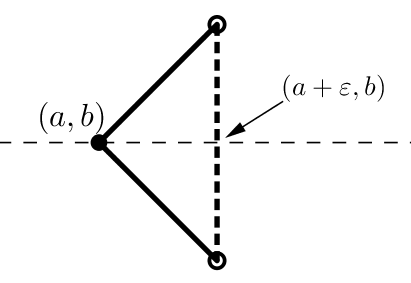
\includegraphics[scale = 1.5]{img/ExamenSeptiembre2017/Abiertosimg}
	\end{figure}
	Estos serán los abiertos de nuestra base de abiertos de la topología $\T$.
	Algo muy importante y que se resaltará siempre es que solo hemos de responder a lo que se nos pide. En este caso ya se nos dice que es una base de la topología, por lo tanto no tenemos que comprobarlo ni nada por el estilo. Podemos jugar con este hecho desde el principio, ya que nos lo da el enunciado.
	\begin{enumerate}
		\item Vamos a hacer una serie de apreciaciones antes de proceder a la resolución de este apartado. Hemos de observar que $\T_u \varsubsetneq \T$. Esto implica que la topología $\T$ es más fina que la usual. Esto se desprende de que cualquier abierto de de la usual contiene un abierto de $\T$, y que esta contención es estricta de que los triángulos no son abiertos en la usual.(La otra contención no se da ya que no podemos meter abiertos de la usual para ciertos puntos del triángulo, como por ejemplo el vértice).
		
		Vamos a calcular entonces la \tb{adherencia de un triángulo semiabierto}. La primera idea intuitiva que nos surge es añadirle al abierto el segmento vertical con los extremos incluidos que une los dos vértices del triángulo.
		
		\begin{figure}[h!]
			\centering
			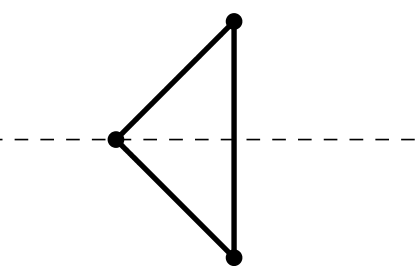
\includegraphics[scale = 1.5]{img/ExamenSeptiembre2017/Abiertosadherencia1img}
		\end{figure}
	
		Estos son cerrados en la topología usual, $\implies$ $\U \subset \adher{U}^{usual}$, luego  $\U \subset \adher{U}^{usual} \subset \adher{U}$.
		Ahora vamos a ver si los puntos que hemos añadido son adherentes. A esto respondemos que no (si llamamos $r$ al segmento citado), ya que $\forall p \in r , \exists V$ entorno de $p \tq \V \cap \U = \emptyset$.
		
		\begin{figure}[h!]
			\centering
			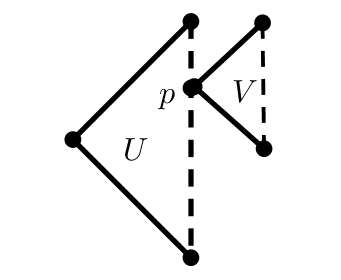
\includegraphics[scale = 1.5]{img/ExamenSeptiembre2017/Abiertosadherencia2img}
		\end{figure}
		
		Por lo tanto la adherencia de $\U$ en esta topología es el propio $\U$, ya que como hemos visto, los puntos de ese segmento no son adherentes.
		
		Si lo hubieramos visto comprobando ``uno a uno" todos los puntos habría que decir además que los puntos de fuera del triángulo no son adherentes ya que existe un abierto en la usual que contiene un triángulo (que es entorno que no corta al conjunto).
		
		Luego  $\adher{\U} = \U$ , lo que implica además que es una base de abiertos y cerrados simultáneamente.
		
		\item Veamos si el espacio topológico es \tb{Lindelöf} \ref{lindel} con esta topología.
		
		Lo primero que tenemos que intentar hacer es ver si hay subespacios especiales (por ejemplo rectas verticales).
		
		Tomamos la recta vertical $r$, subespacio de nuestro espacio topológico con la topología relativa. Si lo cortamos con los abiertos relativos, observamos que $p = r \cap \U^{abierto\ rel.\ en\ r} \implies \T|_r$ es la topología discreta $\implies$ No es II axioma por ser recta con topología discreta $\implies r= \cup_{p\in r}\{p\}$.
		
		Por lo tanto $\T$ no puede ser II axioma, ya que esta es una propiedad hereditaria. Además, $\T$ tampoco es Lindelöf ya que esta es una propiedad hereditaria para cerrados. Como $r$ es cerrado, $\T$ tampoco es Lindelöf.
		
		Para comprobar si es \tb{localmente compacto} procederemos del siguiente modo. Nos hacemos la pregunta, ¿existirá algún entorno compacto?.Supongamos que existe algún entorno compacto $\K^p$. $\exists \K^p \supset \U = \adher{U} \implies \U$ compacto. Nos centraremos en ello.
		Si la respuesta fuera negativa, si encuentro un $\L^{cerrado} \subset \U$ que no es compacto habremos terminado.
		Si tomamos un segmento con los extremos contenidos, vertical, y contenido en un triángulo al que llamaremos $\mathcal{I}$. Si $\exists \K^p \supset \U \supset \mathcal{I}$, la topología de este segmento es la discreta por ser un subespacio de el $r$ que tomamos antes. Además es cerrado en la topología usual. Por lo tanto, $\T|_\mathcal{I}$ es la topología discreta $\implies$ no es compacto (no hay un subrecubrimiento finito), luego hemos terminado ya que al $\mathcal{I}$ no ser compacto no puede existir el supuesto compacto que supusimos.
		\item Veamos si es totalmente disconexo.
		
		Como se vió en resultados teóricos, si un espacio tiene una base \ti{clopen} y es $T_0$ entonces es totalmente disconexo.
		
		SUpongamos que $p,q \in \X, p \neq q\ y\ p,q \in \mathcal{C}$. Veamos que $\mathcal{C}$ no es conexo. Ponemos $\mathcal{C} = (\mathcal{C} \cap \U) \cup (\mathcal{C} \setminus \U)$, sabemos que $\U$ es abierto ambiente ($\U$ es abierto de uno de los puntos que no tiene al otro, que existe por ser $T_0$), y que estas intersecciones son no vacías ya que contienen a los puntos $p$ y $q$. Por lo tanto tenemos dos cerrados que producen la desconexión, y como es para cualquiera dos puntos, el espacio es totalmente disconexo con esta topología. Además se necesita que haya dos puntos distintos.
	
		\item Para ver si algo es topología producto hemos de mirar los productos que lo conforman.
	\end{enumerate}	
\end{proof}
	%%Cosas Pendientes de Manuel Navarro García

\textbf{Número 1.1.} Sea $X$ un conjunto, y $\T_{\text{CF}}$ la familia de todos los subconjuntos de $X$ cuyo complementario es finito, más el conjunto vacío. Probar que $\T_{\text{CF}}$ es una topología en $X$. Esta topología se llama, por razones evidentes, \textit{topología de los complementarios finitos}. ?`Qué topología obtenemos si $X$ es un conjunto finito?  \\

A partir del enunciado se deduce que los abiertos de esta topología son los elementos de la colección 

\[\T_{\text{CF}}= \{U \subset X : U= \emptyset \text{ o } X \backslash U\equiv U^c \text{ es finito}\}.\]

Veamos que efectivamente $\T_{\text{CF}}$ es una topología al verificar las condiciones necesarias. 

\begin{itemize}
\item En primer lugar, el vacío pertenece a esta por definición. Además, el complementario del total $X$ (el vacío) es finito, luego $X$ también pertenece a $\T_{\text{CF}}$. 

\item Por otro lado, sea $\{U_\alpha\}_{\alpha \in I}$ para un cierto conjunto de índices $I$ una colección arbitraria de elementos de $\T_{\text{CF}}$, teniéndose que 

\[X \backslash \bigcup_{\alpha}U_\alpha = \bigcap_{\alpha} (X\backslash U_\alpha).\]

Pero $X-U_\alpha$ es finito para cada $\alpha \in I$, luego la intersección numerable de ellos también lo será. De este modo, la unión numerable de abiertos de $\T_{\text{CF}}$ pertenece a ella.

\item Por último, consideremos $U_1$ y $U_2$ dos abiertos de $\T_{\text{CF}}$. Analógamente al caso anterior, 

\[X \backslash (U_1 \cap U_2) = \bigcup_{i=1}^2 (X\backslash U_i).\]

Sin embargo, $X \backslash U_i$ es finito para $i\in\{1,2\}$, luego la unión finita de conjuntos finitos es finita.
\end{itemize}

Para finalizar, se nos pregunta qué topología se obtendría en caso de que $X$ fuese un conjunto finito. Si damos por cierta esta suposición, es claro que $\T_{\text{CF}}$ coincide con la topología discreta, ya que el complementario de todo conjunto es finito. \\

A pesar de haber terminado con lo requerido del ejercicio, podemos ir más allá estudiando más a fondo esta topología. Para comenzar, nótese que si $X$ es numerable trivialmente el conjunto es separable y primer y segundo axioma de numerabilidad. El caso en el que $X$ no es numerable ya no es tan sencillo. Vayamos por partes.

\begin{itemize}
\item $X$ es separable. Es más, todo conjunto numerable es denso en $X$. En efecto, supongamos que existiese un conjunto $A \subset X$ numerable pero que no es denso en $X$. Esto implica que existe un abierto $B\in \T_{\text{CF}}$ tal que $B\cap A = \emptyset$. De este modo, 

\[(X\backslash B)\cup (X\backslash A)=X.\]

Pero los conjuntos del primer miembro son finitos, y la unión de finitos es finita, lo que conllevaría a que $X$ también lo sea. Esto nos conduce a la  contradicción buscada. 

\item $X$ no es primer axioma de numerabilidad, lo que implica que tampoco es segundo. Para corroborar esto, comprobemos que para cada punto $a\in X$ no existe una base de entornos abiertos numerable centrada en $a$. Razonaremos de nuevo por reducción al absurdo. \\

Supongamos que sí que existe esa base y sea esta 

\[\mathcal{U}^a=\{V_k \in\T_{\text{CF}}: k \geq 1\}.\]

La intersección 

\[\left(\bigcap_{k\geq 1} V_k\right)\backslash \{a\}\]

es no vacía puesto que, al tomar los complementarios y aplicar las leyes de De Morgan se tiene que 

\[X \backslash \left(\bigcap_{k\geq 1} V_k\right)= \left(\bigcup_{k\geq 1} X \backslash V_k\right), \]

y esta unión es numerable ya que $X \backslash V_k$ es finito (recordemos que $V_k \in \T_{\text{CF}}$). Al ser $X$ no numerable y 

\[X= \left(\bigcap_{k\geq 1} V_k\right) \cup \left(\bigcup_{k\geq 1} X\backslash V_k\right),\]

la intersección anterior ha de ser no numerable. \\

Tomemos ahora un punto cualquiera $b$ de esta intersección con la condición de que sea distinto de $a$ y consideremos el entorno abierto de $a$ dado por $W:=X\backslash \{b\}$. Claramente, $a\in W$ y es abierto puesto que su complementario es finito.  De forma evidente la condición $V_k \subset W$ no se verifica para ningún $k$ ya que $b\in V_k$ para todo $k$. Esto verifica que $\mathcal{U}^a$ no puede ser base, concluyendo así que cuando $X$ no es numerable $\T_{\text{CF}}$ no es primer axioma de numerabilidad.

\item $X$ es compacto. En efecto, supongamos que $\{V_k : k \geq 1\}$ es un recubrimiento por abiertos de $X$ y tomemos un $V_{k_0}$ arbitrario. Como este abierto pertenece a $\T_{\text{CF}}$ su complementario es finito, luego 

\[X \backslash V_{k_0} := \{x_1, \ldots, x_r\}\]

con $x_j \in X$ y $j=\{1,\ldots, r\}$ tales que $x_j\in V_{k_j}$ para cierto $k_j$, pues la unión de $V_k$ recubre $X$ según lo hemos definido. De este modo, podemos tomar $X$ como la unión de $V_{k_0}$ con los $V_{k_j}$ que contienen a los puntos $x_j$, esto es,

\[X=\bigcup_{j=0}^r V_{k_j},\]

lo que prueba que $X$ es compacto. 

\item $X$ es conexo. Un modo de probar esto es comprobar que no existen conjuntos abiertos y cerrados simultáneamente. En caso de que esto ocurriese, lo que quiere decir que $A\in \T_{\text{CF}}$ y $X\backslash A \in \T_{\text{CF}}$, se tiene que $X \backslash A$ y $X\backslash (X\backslash A)=A$ son finitos, luego

\[X=A \cup (X\backslash A)\]

sería finito, y esto contradice que sea no numerable. 
\end{itemize}

	%%Cosas Pendientes de Álvaro Rodríguez García

%%%%%%%%%%
% Día 28/2
%%%%%%%%%%

% Después del primer cacho de imágenes directas
	%%Cosas Pendientes de Clara Rodríguez Núñez
	
	%-----Mierdas Varias-----
	%%Basurero donde se ponen cosas que no se sabe muy bien donde poner.
	\backmatter
	\printindex[general]
	\printindex[topologias]
\end{document}